\section{包围盒层次}\label{sec:包围盒层次}

\keyindex{包围盒层次}{bounding volume hierarchy}{}(BVH)是一种
基于图元细分的光线相交加速方法,把图元划分为不相交集合的层次
(相反,空间细分一般把空间划分为不相交集合的层次)。
\reffig{4.2}展示了简单场景的包围盒层次\sidenote{译者注:包围盒是边界框的近义词。}。
图元存于\keyindex{叶子}{leaf}{}中,只要它不与节点的边界相交,
该节点下的子树就可以跳过。
\begin{figure}[htbp]
    \centering%LaTeX with PSTricks extensions
%%Creator: Inkscape 1.0.1 (3bc2e813f5, 2020-09-07)
%%Please note this file requires PSTricks extensions
\psset{xunit=.5pt,yunit=.5pt,runit=.5pt}
\begin{pspicture}(486.5,540.53997803)
{
\newrgbcolor{curcolor}{1 1 1}
\pscustom[linestyle=none,fillstyle=solid,fillcolor=curcolor]
{
\newpath
\moveto(180.18,305.85997803)
\curveto(196.22939482,305.85997803)(209.24,318.8705832)(209.24,334.91997803)
\curveto(209.25213323,346.69122324)(202.16899365,357.30966361)(191.29629426,361.81967461)
\curveto(180.42361715,366.32967637)(167.90482511,363.84214428)(159.58132943,355.5186486)
\curveto(141.2463808,337.18369997)(154.24731849,305.83324788)(180.18,305.85997803)
\closepath
}
}
{
\newrgbcolor{curcolor}{0 0 0}
\pscustom[linestyle=none,fillstyle=solid,fillcolor=curcolor]
{
\newpath
\moveto(180.18,363.47997803)
\curveto(164.40674755,363.47997803)(151.62,350.69323048)(151.62,334.91997803)
\curveto(151.58435925,309.41906014)(182.41250553,296.62810038)(200.44219159,314.65778644)
\curveto(208.6268344,322.84242924)(211.07179876,335.15289509)(206.63507228,345.84337979)
\curveto(202.19833667,356.53388644)(191.75487179,363.49615537)(180.18,363.47997803)
\moveto(180.18,364.47997803)
\curveto(196.5055372,364.47997803)(209.74,351.24551523)(209.74,334.91997803)
\curveto(209.73109046,308.59673601)(177.90714815,295.42494182)(159.29605597,314.036034)
\curveto(140.68496379,332.64712618)(153.85675798,364.47106848)(180.18,364.47997803)
\closepath
}
}
{
\newrgbcolor{curcolor}{1 1 1}
\pscustom[linestyle=none,fillstyle=solid,fillcolor=curcolor]
{
\newpath
\moveto(224.76,419.38997803)
\lineto(290.16,398.63997803)
\lineto(239.49,352.36997803)
\closepath
}
}
{
\newrgbcolor{curcolor}{0 0 0}
\pscustom[linestyle=none,fillstyle=solid,fillcolor=curcolor]
{
\newpath
\moveto(225.43,418.64997803)
\lineto(257.31,408.53997803)
\lineto(289.19,398.42997803)
\lineto(264.49,375.87997803)
\lineto(239.79,353.32997803)
\lineto(232.61,385.99997803)
\lineto(225.43,418.65997803)
\moveto(224.08,420.13997803)
\lineto(231.63,385.77997803)
\lineto(239.19,351.42997803)
\lineto(265.19,375.13997803)
\lineto(291.19,398.85997803)
\lineto(257.66,409.49997803)
\lineto(224.13,420.13997803)
\closepath
}
}
{
\newrgbcolor{curcolor}{1 1 1}
\pscustom[linestyle=none,fillstyle=solid,fillcolor=curcolor]
{
\newpath
\moveto(304.78,536.08997803)
\lineto(383.02,495.40997803)
\lineto(413.91,415.93997803)
\closepath
}
}
{
\newrgbcolor{curcolor}{0 0 0}
\pscustom[linestyle=none,fillstyle=solid,fillcolor=curcolor]
{
\newpath
\moveto(307,534.34997803)
\lineto(342.48,515.90997803)
\lineto(382.59,495.05997803)
\lineto(398.42,454.32997803)
\lineto(412.42,418.26997803)
\lineto(359.68,476.37997803)
\lineto(307,534.34997803)
\moveto(302.5,537.81997803)
\lineto(358.91,475.70997803)
\lineto(415.32,413.59997803)
\lineto(399.32,454.68997803)
\lineto(383.32,495.76997803)
\lineto(343,516.78997803)
\lineto(302.56,537.78997803)
\closepath
}
}
{
\newrgbcolor{curcolor}{0 0 0}
\pscustom[linestyle=none,fillstyle=solid,fillcolor=curcolor]
{
\newpath
\moveto(416.22,538.79997803)
\lineto(414.22,538.79997803)
\lineto(414.22,537.79997803)
\lineto(416.22,537.79997803)
\closepath
\moveto(412.22,538.79997803)
\lineto(410.22,538.79997803)
\lineto(410.22,537.79997803)
\lineto(412.22,537.79997803)
\closepath
\moveto(408.22,538.79997803)
\lineto(406.22,538.79997803)
\lineto(406.22,537.79997803)
\lineto(408.22,537.79997803)
\closepath
\moveto(404.22,538.79997803)
\lineto(402.22,538.79997803)
\lineto(402.22,537.79997803)
\lineto(404.22,537.79997803)
\closepath
\moveto(400.22,538.79997803)
\lineto(398.22,538.79997803)
\lineto(398.22,537.79997803)
\lineto(400.22,537.79997803)
\closepath
\moveto(396.22,538.79997803)
\lineto(394.22,538.79997803)
\lineto(394.22,537.79997803)
\lineto(396.22,537.79997803)
\closepath
\moveto(392.22,538.79997803)
\lineto(390.22,538.79997803)
\lineto(390.22,537.79997803)
\lineto(392.22,537.79997803)
\closepath
\moveto(388.22,538.79997803)
\lineto(386.22,538.79997803)
\lineto(386.22,537.79997803)
\lineto(388.22,537.79997803)
\closepath
\moveto(384.22,538.79997803)
\lineto(382.22,538.79997803)
\lineto(382.22,537.79997803)
\lineto(384.22,537.79997803)
\closepath
\moveto(380.22,538.79997803)
\lineto(378.22,538.79997803)
\lineto(378.22,537.79997803)
\lineto(380.22,537.79997803)
\closepath
\moveto(376.22,538.79997803)
\lineto(374.22,538.79997803)
\lineto(374.22,537.79997803)
\lineto(376.22,537.79997803)
\closepath
\moveto(372.22,538.79997803)
\lineto(370.22,538.79997803)
\lineto(370.22,537.79997803)
\lineto(372.22,537.79997803)
\closepath
\moveto(368.22,538.79997803)
\lineto(366.22,538.79997803)
\lineto(366.22,537.79997803)
\lineto(368.22,537.79997803)
\closepath
\moveto(364.22,538.79997803)
\lineto(362.22,538.79997803)
\lineto(362.22,537.79997803)
\lineto(364.22,537.79997803)
\closepath
\moveto(360.22,538.79997803)
\lineto(358.22,538.79997803)
\lineto(358.22,537.79997803)
\lineto(360.22,537.79997803)
\closepath
\moveto(356.22,538.79997803)
\lineto(354.22,538.79997803)
\lineto(354.22,537.79997803)
\lineto(356.22,537.79997803)
\closepath
\moveto(352.22,538.79997803)
\lineto(350.22,538.79997803)
\lineto(350.22,537.79997803)
\lineto(352.22,537.79997803)
\closepath
\moveto(348.22,538.79997803)
\lineto(346.22,538.79997803)
\lineto(346.22,537.79997803)
\lineto(348.22,537.79997803)
\closepath
\moveto(344.22,538.79997803)
\lineto(342.22,538.79997803)
\lineto(342.22,537.79997803)
\lineto(344.22,537.79997803)
\closepath
\moveto(340.22,538.79997803)
\lineto(338.22,538.79997803)
\lineto(338.22,537.79997803)
\lineto(340.22,537.79997803)
\closepath
\moveto(336.22,538.79997803)
\lineto(334.22,538.79997803)
\lineto(334.22,537.79997803)
\lineto(336.22,537.79997803)
\closepath
\moveto(332.22,538.79997803)
\lineto(330.22,538.79997803)
\lineto(330.22,537.79997803)
\lineto(332.22,537.79997803)
\closepath
\moveto(328.22,538.79997803)
\lineto(326.22,538.79997803)
\lineto(326.22,537.79997803)
\lineto(328.22,537.79997803)
\closepath
\moveto(324.22,538.79997803)
\lineto(322.22,538.79997803)
\lineto(322.22,537.79997803)
\lineto(324.22,537.79997803)
\closepath
\moveto(320.22,538.79997803)
\lineto(318.22,538.79997803)
\lineto(318.22,537.79997803)
\lineto(320.22,537.79997803)
\closepath
\moveto(316.22,538.79997803)
\lineto(314.22,538.79997803)
\lineto(314.22,537.79997803)
\lineto(316.22,537.79997803)
\closepath
\moveto(312.22,538.79997803)
\lineto(310.22,538.79997803)
\lineto(310.22,537.79997803)
\lineto(312.22,537.79997803)
\closepath
\moveto(308.22,538.79997803)
\lineto(306.22,538.79997803)
\lineto(306.22,537.79997803)
\lineto(308.22,537.79997803)
\closepath
\moveto(304.22,538.79997803)
\lineto(302.22,538.79997803)
\lineto(302.22,537.79997803)
\lineto(304.22,537.79997803)
\closepath
\moveto(302.46,537.53997803)
\lineto(301.46,537.53997803)
\lineto(301.46,535.53997803)
\lineto(302.46,535.53997803)
\closepath
\moveto(302.46,533.53997803)
\lineto(301.46,533.53997803)
\lineto(301.46,531.53997803)
\lineto(302.46,531.53997803)
\closepath
\moveto(302.46,529.53997803)
\lineto(301.46,529.53997803)
\lineto(301.46,527.53997803)
\lineto(302.46,527.53997803)
\closepath
\moveto(302.46,525.53997803)
\lineto(301.46,525.53997803)
\lineto(301.46,523.53997803)
\lineto(302.46,523.53997803)
\closepath
\moveto(302.46,521.53997803)
\lineto(301.46,521.53997803)
\lineto(301.46,519.53997803)
\lineto(302.46,519.53997803)
\closepath
\moveto(302.46,517.53997803)
\lineto(301.46,517.53997803)
\lineto(301.46,515.53997803)
\lineto(302.46,515.53997803)
\closepath
\moveto(302.46,513.53997803)
\lineto(301.46,513.53997803)
\lineto(301.46,511.53997803)
\lineto(302.46,511.53997803)
\closepath
\moveto(302.46,509.53997803)
\lineto(301.46,509.53997803)
\lineto(301.46,507.53997803)
\lineto(302.46,507.53997803)
\closepath
\moveto(302.46,505.53997803)
\lineto(301.46,505.53997803)
\lineto(301.46,503.53997803)
\lineto(302.46,503.53997803)
\closepath
\moveto(302.46,501.53997803)
\lineto(301.46,501.53997803)
\lineto(301.46,499.53997803)
\lineto(302.46,499.53997803)
\closepath
\moveto(302.46,497.53997803)
\lineto(301.46,497.53997803)
\lineto(301.46,495.53997803)
\lineto(302.46,495.53997803)
\closepath
\moveto(302.46,493.53997803)
\lineto(301.46,493.53997803)
\lineto(301.46,491.53997803)
\lineto(302.46,491.53997803)
\closepath
\moveto(302.46,489.53997803)
\lineto(301.46,489.53997803)
\lineto(301.46,487.53997803)
\lineto(302.46,487.53997803)
\closepath
\moveto(302.46,485.53997803)
\lineto(301.46,485.53997803)
\lineto(301.46,483.53997803)
\lineto(302.46,483.53997803)
\closepath
\moveto(302.46,481.53997803)
\lineto(301.46,481.53997803)
\lineto(301.46,479.53997803)
\lineto(302.46,479.53997803)
\closepath
\moveto(302.46,477.53997803)
\lineto(301.46,477.53997803)
\lineto(301.46,475.53997803)
\lineto(302.46,475.53997803)
\closepath
\moveto(302.46,473.53997803)
\lineto(301.46,473.53997803)
\lineto(301.46,471.53997803)
\lineto(302.46,471.53997803)
\closepath
\moveto(302.46,469.53997803)
\lineto(301.46,469.53997803)
\lineto(301.46,467.53997803)
\lineto(302.46,467.53997803)
\closepath
\moveto(302.46,465.53997803)
\lineto(301.46,465.53997803)
\lineto(301.46,463.53997803)
\lineto(302.46,463.53997803)
\closepath
\moveto(302.46,461.53997803)
\lineto(301.46,461.53997803)
\lineto(301.46,459.53997803)
\lineto(302.46,459.53997803)
\closepath
\moveto(302.46,457.53997803)
\lineto(301.46,457.53997803)
\lineto(301.46,455.53997803)
\lineto(302.46,455.53997803)
\closepath
\moveto(302.46,453.53997803)
\lineto(301.46,453.53997803)
\lineto(301.46,451.53997803)
\lineto(302.46,451.53997803)
\closepath
\moveto(302.46,449.53997803)
\lineto(301.46,449.53997803)
\lineto(301.46,447.53997803)
\lineto(302.46,447.53997803)
\closepath
\moveto(302.46,445.53997803)
\lineto(301.46,445.53997803)
\lineto(301.46,443.53997803)
\lineto(302.46,443.53997803)
\closepath
\moveto(302.46,441.53997803)
\lineto(301.46,441.53997803)
\lineto(301.46,439.53997803)
\lineto(302.46,439.53997803)
\closepath
\moveto(302.46,437.53997803)
\lineto(301.46,437.53997803)
\lineto(301.46,435.53997803)
\lineto(302.46,435.53997803)
\closepath
\moveto(302.46,433.53997803)
\lineto(301.46,433.53997803)
\lineto(301.46,431.53997803)
\lineto(302.46,431.53997803)
\closepath
\moveto(302.46,429.53997803)
\lineto(301.46,429.53997803)
\lineto(301.46,427.53997803)
\lineto(302.46,427.53997803)
\closepath
\moveto(302.46,425.53997803)
\lineto(301.46,425.53997803)
\lineto(301.46,423.53997803)
\lineto(302.46,423.53997803)
\closepath
\moveto(302.46,421.53997803)
\lineto(301.46,421.53997803)
\lineto(301.46,419.53997803)
\lineto(302.46,419.53997803)
\closepath
\moveto(302.46,417.53997803)
\lineto(301.46,417.53997803)
\lineto(301.46,415.53997803)
\lineto(302.46,415.53997803)
\closepath
\moveto(303.94,415.01997803)
\lineto(301.94,415.01997803)
\lineto(301.94,414.01997803)
\lineto(303.94,414.01997803)
\closepath
\moveto(307.94,415.01997803)
\lineto(305.94,415.01997803)
\lineto(305.94,414.01997803)
\lineto(307.94,414.01997803)
\closepath
\moveto(311.94,415.01997803)
\lineto(309.94,415.01997803)
\lineto(309.94,414.01997803)
\lineto(311.94,414.01997803)
\closepath
\moveto(315.94,415.01997803)
\lineto(313.94,415.01997803)
\lineto(313.94,414.01997803)
\lineto(315.94,414.01997803)
\closepath
\moveto(319.94,415.01997803)
\lineto(317.94,415.01997803)
\lineto(317.94,414.01997803)
\lineto(319.94,414.01997803)
\closepath
\moveto(323.94,415.01997803)
\lineto(321.94,415.01997803)
\lineto(321.94,414.01997803)
\lineto(323.94,414.01997803)
\closepath
\moveto(327.94,415.01997803)
\lineto(325.94,415.01997803)
\lineto(325.94,414.01997803)
\lineto(327.94,414.01997803)
\closepath
\moveto(331.94,415.01997803)
\lineto(329.94,415.01997803)
\lineto(329.94,414.01997803)
\lineto(331.94,414.01997803)
\closepath
\moveto(335.94,415.01997803)
\lineto(333.94,415.01997803)
\lineto(333.94,414.01997803)
\lineto(335.94,414.01997803)
\closepath
\moveto(339.94,415.01997803)
\lineto(337.94,415.01997803)
\lineto(337.94,414.01997803)
\lineto(339.94,414.01997803)
\closepath
\moveto(343.94,415.01997803)
\lineto(341.94,415.01997803)
\lineto(341.94,414.01997803)
\lineto(343.94,414.01997803)
\closepath
\moveto(347.94,415.01997803)
\lineto(345.94,415.01997803)
\lineto(345.94,414.01997803)
\lineto(347.94,414.01997803)
\closepath
\moveto(351.94,415.01997803)
\lineto(349.94,415.01997803)
\lineto(349.94,414.01997803)
\lineto(351.94,414.01997803)
\closepath
\moveto(355.94,415.01997803)
\lineto(353.94,415.01997803)
\lineto(353.94,414.01997803)
\lineto(355.94,414.01997803)
\closepath
\moveto(359.94,415.01997803)
\lineto(357.94,415.01997803)
\lineto(357.94,414.01997803)
\lineto(359.94,414.01997803)
\closepath
\moveto(363.94,415.01997803)
\lineto(361.94,415.01997803)
\lineto(361.94,414.01997803)
\lineto(363.94,414.01997803)
\closepath
\moveto(367.94,415.01997803)
\lineto(365.94,415.01997803)
\lineto(365.94,414.01997803)
\lineto(367.94,414.01997803)
\closepath
\moveto(371.94,415.01997803)
\lineto(369.94,415.01997803)
\lineto(369.94,414.01997803)
\lineto(371.94,414.01997803)
\closepath
\moveto(375.94,415.01997803)
\lineto(373.94,415.01997803)
\lineto(373.94,414.01997803)
\lineto(375.94,414.01997803)
\closepath
\moveto(379.94,415.01997803)
\lineto(377.94,415.01997803)
\lineto(377.94,414.01997803)
\lineto(379.94,414.01997803)
\closepath
\moveto(383.94,415.01997803)
\lineto(381.94,415.01997803)
\lineto(381.94,414.01997803)
\lineto(383.94,414.01997803)
\closepath
\moveto(387.94,415.01997803)
\lineto(385.94,415.01997803)
\lineto(385.94,414.01997803)
\lineto(387.94,414.01997803)
\closepath
\moveto(391.94,415.01997803)
\lineto(389.94,415.01997803)
\lineto(389.94,414.01997803)
\lineto(391.94,414.01997803)
\closepath
\moveto(395.94,415.01997803)
\lineto(393.94,415.01997803)
\lineto(393.94,414.01997803)
\lineto(395.94,414.01997803)
\closepath
\moveto(399.94,415.01997803)
\lineto(397.94,415.01997803)
\lineto(397.94,414.01997803)
\lineto(399.94,414.01997803)
\closepath
\moveto(403.94,415.01997803)
\lineto(401.94,415.01997803)
\lineto(401.94,414.01997803)
\lineto(403.94,414.01997803)
\closepath
\moveto(407.94,415.01997803)
\lineto(405.94,415.01997803)
\lineto(405.94,414.01997803)
\lineto(407.94,414.01997803)
\closepath
\moveto(411.94,415.01997803)
\lineto(409.94,415.01997803)
\lineto(409.94,414.01997803)
\lineto(411.94,414.01997803)
\closepath
\moveto(415.94,415.01997803)
\lineto(413.94,415.01997803)
\lineto(413.94,414.01997803)
\lineto(415.94,414.01997803)
\closepath
\moveto(416.22,417.72997803)
\lineto(415.22,417.72997803)
\lineto(415.22,415.72997803)
\lineto(416.22,415.72997803)
\closepath
\moveto(416.22,421.72997803)
\lineto(415.22,421.72997803)
\lineto(415.22,419.72997803)
\lineto(416.22,419.72997803)
\closepath
\moveto(416.22,425.72997803)
\lineto(415.22,425.72997803)
\lineto(415.22,423.72997803)
\lineto(416.22,423.72997803)
\closepath
\moveto(416.22,429.72997803)
\lineto(415.22,429.72997803)
\lineto(415.22,427.72997803)
\lineto(416.22,427.72997803)
\closepath
\moveto(416.22,433.72997803)
\lineto(415.22,433.72997803)
\lineto(415.22,431.72997803)
\lineto(416.22,431.72997803)
\closepath
\moveto(416.22,437.72997803)
\lineto(415.22,437.72997803)
\lineto(415.22,435.72997803)
\lineto(416.22,435.72997803)
\closepath
\moveto(416.22,441.72997803)
\lineto(415.22,441.72997803)
\lineto(415.22,439.72997803)
\lineto(416.22,439.72997803)
\closepath
\moveto(416.22,445.72997803)
\lineto(415.22,445.72997803)
\lineto(415.22,443.72997803)
\lineto(416.22,443.72997803)
\closepath
\moveto(416.22,449.72997803)
\lineto(415.22,449.72997803)
\lineto(415.22,447.72997803)
\lineto(416.22,447.72997803)
\closepath
\moveto(416.22,453.72997803)
\lineto(415.22,453.72997803)
\lineto(415.22,451.72997803)
\lineto(416.22,451.72997803)
\closepath
\moveto(416.22,457.72997803)
\lineto(415.22,457.72997803)
\lineto(415.22,455.72997803)
\lineto(416.22,455.72997803)
\closepath
\moveto(416.22,461.72997803)
\lineto(415.22,461.72997803)
\lineto(415.22,459.72997803)
\lineto(416.22,459.72997803)
\closepath
\moveto(416.22,465.72997803)
\lineto(415.22,465.72997803)
\lineto(415.22,463.72997803)
\lineto(416.22,463.72997803)
\closepath
\moveto(416.22,469.72997803)
\lineto(415.22,469.72997803)
\lineto(415.22,467.72997803)
\lineto(416.22,467.72997803)
\closepath
\moveto(416.22,473.72997803)
\lineto(415.22,473.72997803)
\lineto(415.22,471.72997803)
\lineto(416.22,471.72997803)
\closepath
\moveto(416.22,477.72997803)
\lineto(415.22,477.72997803)
\lineto(415.22,475.72997803)
\lineto(416.22,475.72997803)
\closepath
\moveto(416.22,481.72997803)
\lineto(415.22,481.72997803)
\lineto(415.22,479.72997803)
\lineto(416.22,479.72997803)
\closepath
\moveto(416.22,485.72997803)
\lineto(415.22,485.72997803)
\lineto(415.22,483.72997803)
\lineto(416.22,483.72997803)
\closepath
\moveto(416.22,489.72997803)
\lineto(415.22,489.72997803)
\lineto(415.22,487.72997803)
\lineto(416.22,487.72997803)
\closepath
\moveto(416.22,493.72997803)
\lineto(415.22,493.72997803)
\lineto(415.22,491.72997803)
\lineto(416.22,491.72997803)
\closepath
\moveto(416.22,497.72997803)
\lineto(415.22,497.72997803)
\lineto(415.22,495.72997803)
\lineto(416.22,495.72997803)
\closepath
\moveto(416.22,501.72997803)
\lineto(415.22,501.72997803)
\lineto(415.22,499.72997803)
\lineto(416.22,499.72997803)
\closepath
\moveto(416.22,505.72997803)
\lineto(415.22,505.72997803)
\lineto(415.22,503.72997803)
\lineto(416.22,503.72997803)
\closepath
\moveto(416.22,509.72997803)
\lineto(415.22,509.72997803)
\lineto(415.22,507.72997803)
\lineto(416.22,507.72997803)
\closepath
\moveto(416.22,513.72997803)
\lineto(415.22,513.72997803)
\lineto(415.22,511.72997803)
\lineto(416.22,511.72997803)
\closepath
\moveto(416.22,517.72997803)
\lineto(415.22,517.72997803)
\lineto(415.22,515.72997803)
\lineto(416.22,515.72997803)
\closepath
\moveto(416.22,521.72997803)
\lineto(415.22,521.72997803)
\lineto(415.22,519.72997803)
\lineto(416.22,519.72997803)
\closepath
\moveto(416.22,525.72997803)
\lineto(415.22,525.72997803)
\lineto(415.22,523.72997803)
\lineto(416.22,523.72997803)
\closepath
\moveto(416.22,529.72997803)
\lineto(415.22,529.72997803)
\lineto(415.22,527.72997803)
\lineto(416.22,527.72997803)
\closepath
\moveto(416.22,533.72997803)
\lineto(415.22,533.72997803)
\lineto(415.22,531.72997803)
\lineto(416.22,531.72997803)
\closepath
\moveto(416.22,537.72997803)
\lineto(415.22,537.72997803)
\lineto(415.22,535.72997803)
\lineto(416.22,535.72997803)
\closepath
}
}
{
\newrgbcolor{curcolor}{0 0 0}
\pscustom[linestyle=none,fillstyle=solid,fillcolor=curcolor]
{
\newpath
\moveto(292.33,420.98997803)
\lineto(290.33,420.98997803)
\lineto(290.33,419.98997803)
\lineto(291.33,419.98997803)
\lineto(291.33,418.42997803)
\lineto(292.33,418.42997803)
\closepath
\moveto(288.33,420.98997803)
\lineto(286.33,420.98997803)
\lineto(286.33,419.98997803)
\lineto(288.33,419.98997803)
\closepath
\moveto(284.33,420.98997803)
\lineto(282.33,420.98997803)
\lineto(282.33,419.98997803)
\lineto(284.33,419.98997803)
\closepath
\moveto(280.33,420.98997803)
\lineto(278.33,420.98997803)
\lineto(278.33,419.98997803)
\lineto(280.33,419.98997803)
\closepath
\moveto(276.33,420.98997803)
\lineto(274.33,420.98997803)
\lineto(274.33,419.98997803)
\lineto(276.33,419.98997803)
\closepath
\moveto(272.33,420.98997803)
\lineto(270.33,420.98997803)
\lineto(270.33,419.98997803)
\lineto(272.33,419.98997803)
\closepath
\moveto(268.33,420.98997803)
\lineto(266.33,420.98997803)
\lineto(266.33,419.98997803)
\lineto(268.33,419.98997803)
\closepath
\moveto(264.33,420.98997803)
\lineto(262.33,420.98997803)
\lineto(262.33,419.98997803)
\lineto(264.33,419.98997803)
\closepath
\moveto(260.33,420.98997803)
\lineto(258.33,420.98997803)
\lineto(258.33,419.98997803)
\lineto(260.33,419.98997803)
\closepath
\moveto(256.33,420.98997803)
\lineto(254.33,420.98997803)
\lineto(254.33,419.98997803)
\lineto(256.33,419.98997803)
\closepath
\moveto(252.33,420.98997803)
\lineto(250.33,420.98997803)
\lineto(250.33,419.98997803)
\lineto(252.33,419.98997803)
\closepath
\moveto(248.33,420.98997803)
\lineto(246.33,420.98997803)
\lineto(246.33,419.98997803)
\lineto(248.33,419.98997803)
\closepath
\moveto(244.33,420.98997803)
\lineto(242.33,420.98997803)
\lineto(242.33,419.98997803)
\lineto(244.33,419.98997803)
\closepath
\moveto(240.33,420.98997803)
\lineto(238.33,420.98997803)
\lineto(238.33,419.98997803)
\lineto(240.33,419.98997803)
\closepath
\moveto(236.33,420.98997803)
\lineto(234.33,420.98997803)
\lineto(234.33,419.98997803)
\lineto(236.33,419.98997803)
\closepath
\moveto(232.33,420.98997803)
\lineto(230.33,420.98997803)
\lineto(230.33,419.98997803)
\lineto(232.33,419.98997803)
\closepath
\moveto(228.33,420.98997803)
\lineto(226.33,420.98997803)
\lineto(226.33,419.98997803)
\lineto(228.33,419.98997803)
\closepath
\moveto(224.33,420.98997803)
\lineto(222.33,420.98997803)
\lineto(222.33,419.98997803)
\lineto(224.33,419.98997803)
\closepath
\moveto(222.47,419.84997803)
\lineto(221.47,419.84997803)
\lineto(221.47,417.84997803)
\lineto(222.47,417.84997803)
\closepath
\moveto(222.47,415.84997803)
\lineto(221.47,415.84997803)
\lineto(221.47,413.84997803)
\lineto(222.47,413.84997803)
\closepath
\moveto(222.47,411.84997803)
\lineto(221.47,411.84997803)
\lineto(221.47,409.84997803)
\lineto(222.47,409.84997803)
\closepath
\moveto(222.47,407.84997803)
\lineto(221.47,407.84997803)
\lineto(221.47,405.84997803)
\lineto(222.47,405.84997803)
\closepath
\moveto(222.47,403.84997803)
\lineto(221.47,403.84997803)
\lineto(221.47,401.84997803)
\lineto(222.47,401.84997803)
\closepath
\moveto(222.47,399.84997803)
\lineto(221.47,399.84997803)
\lineto(221.47,397.84997803)
\lineto(222.47,397.84997803)
\closepath
\moveto(222.47,395.84997803)
\lineto(221.47,395.84997803)
\lineto(221.47,393.84997803)
\lineto(222.47,393.84997803)
\closepath
\moveto(222.47,391.84997803)
\lineto(221.47,391.84997803)
\lineto(221.47,389.84997803)
\lineto(222.47,389.84997803)
\closepath
\moveto(222.47,387.84997803)
\lineto(221.47,387.84997803)
\lineto(221.47,385.84997803)
\lineto(222.47,385.84997803)
\closepath
\moveto(222.47,383.84997803)
\lineto(221.47,383.84997803)
\lineto(221.47,381.84997803)
\lineto(222.47,381.84997803)
\closepath
\moveto(222.47,379.84997803)
\lineto(221.47,379.84997803)
\lineto(221.47,377.84997803)
\lineto(222.47,377.84997803)
\closepath
\moveto(222.47,375.84997803)
\lineto(221.47,375.84997803)
\lineto(221.47,373.84997803)
\lineto(222.47,373.84997803)
\closepath
\moveto(222.47,371.84997803)
\lineto(221.47,371.84997803)
\lineto(221.47,369.84997803)
\lineto(222.47,369.84997803)
\closepath
\moveto(222.47,367.84997803)
\lineto(221.47,367.84997803)
\lineto(221.47,365.84997803)
\lineto(222.47,365.84997803)
\closepath
\moveto(222.47,363.84997803)
\lineto(221.47,363.84997803)
\lineto(221.47,361.84997803)
\lineto(222.47,361.84997803)
\closepath
\moveto(222.47,359.84997803)
\lineto(221.47,359.84997803)
\lineto(221.47,357.84997803)
\lineto(222.47,357.84997803)
\closepath
\moveto(222.47,355.84997803)
\lineto(221.47,355.84997803)
\lineto(221.47,353.84997803)
\lineto(222.47,353.84997803)
\closepath
\moveto(222.47,351.84997803)
\lineto(221.47,351.84997803)
\lineto(221.47,350.53997803)
\lineto(222.47,350.53997803)
\lineto(222.47,351.81997803)
\closepath
\moveto(226.19,351.56997803)
\lineto(224.19,351.56997803)
\lineto(224.19,350.56997803)
\lineto(226.19,350.56997803)
\closepath
\moveto(230.19,351.56997803)
\lineto(228.19,351.56997803)
\lineto(228.19,350.56997803)
\lineto(230.19,350.56997803)
\closepath
\moveto(234.19,351.56997803)
\lineto(232.19,351.56997803)
\lineto(232.19,350.56997803)
\lineto(234.19,350.56997803)
\closepath
\moveto(238.19,351.56997803)
\lineto(236.19,351.56997803)
\lineto(236.19,350.56997803)
\lineto(238.19,350.56997803)
\closepath
\moveto(242.19,351.56997803)
\lineto(240.19,351.56997803)
\lineto(240.19,350.56997803)
\lineto(242.19,350.56997803)
\closepath
\moveto(246.19,351.56997803)
\lineto(244.19,351.56997803)
\lineto(244.19,350.56997803)
\lineto(246.19,350.56997803)
\closepath
\moveto(250.19,351.56997803)
\lineto(248.19,351.56997803)
\lineto(248.19,350.56997803)
\lineto(250.19,350.56997803)
\closepath
\moveto(254.19,351.56997803)
\lineto(252.19,351.56997803)
\lineto(252.19,350.56997803)
\lineto(254.19,350.56997803)
\closepath
\moveto(258.19,351.56997803)
\lineto(256.19,351.56997803)
\lineto(256.19,350.56997803)
\lineto(258.19,350.56997803)
\closepath
\moveto(262.19,351.56997803)
\lineto(260.19,351.56997803)
\lineto(260.19,350.56997803)
\lineto(262.19,350.56997803)
\closepath
\moveto(266.19,351.56997803)
\lineto(264.19,351.56997803)
\lineto(264.19,350.56997803)
\lineto(266.19,350.56997803)
\closepath
\moveto(270.19,351.56997803)
\lineto(268.19,351.56997803)
\lineto(268.19,350.56997803)
\lineto(270.19,350.56997803)
\closepath
\moveto(274.19,351.56997803)
\lineto(272.19,351.56997803)
\lineto(272.19,350.56997803)
\lineto(274.19,350.56997803)
\closepath
\moveto(278.19,351.56997803)
\lineto(276.19,351.56997803)
\lineto(276.19,350.56997803)
\lineto(278.19,350.56997803)
\closepath
\moveto(282.19,351.56997803)
\lineto(280.19,351.56997803)
\lineto(280.19,350.56997803)
\lineto(282.19,350.56997803)
\closepath
\moveto(286.19,351.56997803)
\lineto(284.19,351.56997803)
\lineto(284.19,350.56997803)
\lineto(286.19,350.56997803)
\closepath
\moveto(290.19,351.56997803)
\lineto(288.19,351.56997803)
\lineto(288.19,350.56997803)
\lineto(290.19,350.56997803)
\closepath
\moveto(292.33,352.42997803)
\lineto(291.33,352.42997803)
\lineto(291.33,350.53997803)
\lineto(292.33,350.53997803)
\lineto(292.33,352.39997803)
\closepath
\moveto(292.33,356.42997803)
\lineto(291.33,356.42997803)
\lineto(291.33,354.42997803)
\lineto(292.33,354.42997803)
\closepath
\moveto(292.33,360.42997803)
\lineto(291.33,360.42997803)
\lineto(291.33,358.42997803)
\lineto(292.33,358.42997803)
\closepath
\moveto(292.33,364.42997803)
\lineto(291.33,364.42997803)
\lineto(291.33,362.42997803)
\lineto(292.33,362.42997803)
\closepath
\moveto(292.33,368.42997803)
\lineto(291.33,368.42997803)
\lineto(291.33,366.42997803)
\lineto(292.33,366.42997803)
\closepath
\moveto(292.33,372.42997803)
\lineto(291.33,372.42997803)
\lineto(291.33,370.42997803)
\lineto(292.33,370.42997803)
\closepath
\moveto(292.33,376.42997803)
\lineto(291.33,376.42997803)
\lineto(291.33,374.42997803)
\lineto(292.33,374.42997803)
\closepath
\moveto(292.33,380.42997803)
\lineto(291.33,380.42997803)
\lineto(291.33,378.42997803)
\lineto(292.33,378.42997803)
\closepath
\moveto(292.33,384.42997803)
\lineto(291.33,384.42997803)
\lineto(291.33,382.42997803)
\lineto(292.33,382.42997803)
\closepath
\moveto(292.33,388.42997803)
\lineto(291.33,388.42997803)
\lineto(291.33,386.42997803)
\lineto(292.33,386.42997803)
\closepath
\moveto(292.33,392.42997803)
\lineto(291.33,392.42997803)
\lineto(291.33,390.42997803)
\lineto(292.33,390.42997803)
\closepath
\moveto(292.33,396.42997803)
\lineto(291.33,396.42997803)
\lineto(291.33,394.42997803)
\lineto(292.33,394.42997803)
\closepath
\moveto(292.33,400.42997803)
\lineto(291.33,400.42997803)
\lineto(291.33,398.42997803)
\lineto(292.33,398.42997803)
\closepath
\moveto(292.33,404.42997803)
\lineto(291.33,404.42997803)
\lineto(291.33,402.42997803)
\lineto(292.33,402.42997803)
\closepath
\moveto(292.33,408.42997803)
\lineto(291.33,408.42997803)
\lineto(291.33,406.42997803)
\lineto(292.33,406.42997803)
\closepath
\moveto(292.33,412.42997803)
\lineto(291.33,412.42997803)
\lineto(291.33,410.42997803)
\lineto(292.33,410.42997803)
\closepath
\moveto(292.33,416.42997803)
\lineto(291.33,416.42997803)
\lineto(291.33,414.42997803)
\lineto(292.33,414.42997803)
\closepath
}
}
{
\newrgbcolor{curcolor}{0 0 0}
\pscustom[linestyle=none,fillstyle=solid,fillcolor=curcolor]
{
\newpath
\moveto(206.61,366.21997803)
\lineto(204.61,366.21997803)
\lineto(204.61,365.21997803)
\lineto(206.61,365.21997803)
\closepath
\moveto(202.61,366.21997803)
\lineto(200.61,366.21997803)
\lineto(200.61,365.21997803)
\lineto(202.61,365.21997803)
\closepath
\moveto(198.61,366.21997803)
\lineto(196.61,366.21997803)
\lineto(196.61,365.21997803)
\lineto(198.61,365.21997803)
\closepath
\moveto(194.61,366.21997803)
\lineto(192.61,366.21997803)
\lineto(192.61,365.21997803)
\lineto(194.61,365.21997803)
\closepath
\moveto(190.61,366.21997803)
\lineto(188.61,366.21997803)
\lineto(188.61,365.21997803)
\lineto(190.61,365.21997803)
\closepath
\moveto(186.61,366.21997803)
\lineto(184.61,366.21997803)
\lineto(184.61,365.21997803)
\lineto(186.61,365.21997803)
\closepath
\moveto(182.61,366.21997803)
\lineto(180.61,366.21997803)
\lineto(180.61,365.21997803)
\lineto(182.61,365.21997803)
\closepath
\moveto(178.61,366.21997803)
\lineto(176.61,366.21997803)
\lineto(176.61,365.21997803)
\lineto(178.61,365.21997803)
\closepath
\moveto(174.61,366.21997803)
\lineto(172.61,366.21997803)
\lineto(172.61,365.21997803)
\lineto(174.61,365.21997803)
\closepath
\moveto(170.61,366.21997803)
\lineto(168.61,366.21997803)
\lineto(168.61,365.21997803)
\lineto(170.61,365.21997803)
\closepath
\moveto(166.61,366.21997803)
\lineto(164.61,366.21997803)
\lineto(164.61,365.21997803)
\lineto(166.61,365.21997803)
\closepath
\moveto(162.61,366.21997803)
\lineto(160.61,366.21997803)
\lineto(160.61,365.21997803)
\lineto(162.61,365.21997803)
\closepath
\moveto(158.61,366.21997803)
\lineto(156.61,366.21997803)
\lineto(156.61,365.21997803)
\lineto(158.61,365.21997803)
\closepath
\moveto(154.61,366.21997803)
\lineto(152.61,366.21997803)
\lineto(152.61,365.21997803)
\lineto(154.61,365.21997803)
\closepath
\moveto(150.61,366.21997803)
\lineto(148.88,366.21997803)
\lineto(148.88,365.21997803)
\lineto(150.61,365.21997803)
\closepath
\moveto(149.88,363.94997803)
\lineto(148.88,363.94997803)
\lineto(148.88,361.94997803)
\lineto(149.88,361.94997803)
\closepath
\moveto(149.88,359.94997803)
\lineto(148.88,359.94997803)
\lineto(148.88,357.94997803)
\lineto(149.88,357.94997803)
\closepath
\moveto(149.88,355.94997803)
\lineto(148.88,355.94997803)
\lineto(148.88,353.94997803)
\lineto(149.88,353.94997803)
\closepath
\moveto(149.88,351.94997803)
\lineto(148.88,351.94997803)
\lineto(148.88,349.94997803)
\lineto(149.88,349.94997803)
\closepath
\moveto(149.88,347.94997803)
\lineto(148.88,347.94997803)
\lineto(148.88,345.94997803)
\lineto(149.88,345.94997803)
\closepath
\moveto(149.88,343.94997803)
\lineto(148.88,343.94997803)
\lineto(148.88,341.94997803)
\lineto(149.88,341.94997803)
\closepath
\moveto(149.88,339.94997803)
\lineto(148.88,339.94997803)
\lineto(148.88,337.94997803)
\lineto(149.88,337.94997803)
\closepath
\moveto(149.88,335.94997803)
\lineto(148.88,335.94997803)
\lineto(148.88,333.94997803)
\lineto(149.88,333.94997803)
\closepath
\moveto(149.88,331.94997803)
\lineto(148.88,331.94997803)
\lineto(148.88,329.94997803)
\lineto(149.88,329.94997803)
\closepath
\moveto(149.88,327.94997803)
\lineto(148.88,327.94997803)
\lineto(148.88,325.94997803)
\lineto(149.88,325.94997803)
\closepath
\moveto(149.88,323.94997803)
\lineto(148.88,323.94997803)
\lineto(148.88,321.94997803)
\lineto(149.88,321.94997803)
\closepath
\moveto(149.88,319.94997803)
\lineto(148.88,319.94997803)
\lineto(148.88,317.94997803)
\lineto(149.88,317.94997803)
\closepath
\moveto(149.88,315.94997803)
\lineto(148.88,315.94997803)
\lineto(148.88,313.94997803)
\lineto(149.88,313.94997803)
\closepath
\moveto(149.88,311.94997803)
\lineto(148.88,311.94997803)
\lineto(148.88,309.94997803)
\lineto(149.88,309.94997803)
\closepath
\moveto(149.88,307.94997803)
\lineto(148.88,307.94997803)
\lineto(148.88,305.94997803)
\lineto(149.88,305.94997803)
\closepath
\moveto(150.55,304.61997803)
\lineto(148.88,304.61997803)
\lineto(148.88,303.94997803)
\lineto(148.88,303.94997803)
\lineto(148.88,303.94997803)
\lineto(148.88,303.94997803)
\lineto(148.88,303.61997803)
\lineto(150.55,303.61997803)
\closepath
\moveto(154.55,304.61997803)
\lineto(152.55,304.61997803)
\lineto(152.55,303.61997803)
\lineto(154.55,303.61997803)
\closepath
\moveto(158.55,304.61997803)
\lineto(156.55,304.61997803)
\lineto(156.55,303.61997803)
\lineto(158.55,303.61997803)
\closepath
\moveto(162.55,304.61997803)
\lineto(160.55,304.61997803)
\lineto(160.55,303.61997803)
\lineto(162.55,303.61997803)
\closepath
\moveto(166.55,304.61997803)
\lineto(164.55,304.61997803)
\lineto(164.55,303.61997803)
\lineto(166.55,303.61997803)
\closepath
\moveto(170.55,304.61997803)
\lineto(168.55,304.61997803)
\lineto(168.55,303.61997803)
\lineto(170.55,303.61997803)
\closepath
\moveto(174.55,304.61997803)
\lineto(172.55,304.61997803)
\lineto(172.55,303.61997803)
\lineto(174.55,303.61997803)
\closepath
\moveto(178.55,304.61997803)
\lineto(176.55,304.61997803)
\lineto(176.55,303.61997803)
\lineto(178.55,303.61997803)
\closepath
\moveto(182.55,304.61997803)
\lineto(180.55,304.61997803)
\lineto(180.55,303.61997803)
\lineto(182.55,303.61997803)
\closepath
\moveto(186.55,304.61997803)
\lineto(184.55,304.61997803)
\lineto(184.55,303.61997803)
\lineto(186.55,303.61997803)
\closepath
\moveto(190.55,304.61997803)
\lineto(188.55,304.61997803)
\lineto(188.55,303.61997803)
\lineto(190.55,303.61997803)
\closepath
\moveto(194.55,304.61997803)
\lineto(192.55,304.61997803)
\lineto(192.55,303.61997803)
\lineto(194.55,303.61997803)
\closepath
\moveto(198.55,304.61997803)
\lineto(196.55,304.61997803)
\lineto(196.55,303.61997803)
\lineto(198.55,303.61997803)
\closepath
\moveto(202.55,304.61997803)
\lineto(200.55,304.61997803)
\lineto(200.55,303.61997803)
\lineto(202.55,303.61997803)
\closepath
\moveto(206.55,304.61997803)
\lineto(204.55,304.61997803)
\lineto(204.55,303.61997803)
\lineto(206.55,303.61997803)
\closepath
\moveto(210.55,304.61997803)
\lineto(208.55,304.61997803)
\lineto(208.55,303.61997803)
\lineto(210.55,303.61997803)
\closepath
\moveto(210.61,307.56997803)
\lineto(209.61,307.56997803)
\lineto(209.61,305.56997803)
\lineto(210.61,305.56997803)
\closepath
\moveto(210.61,311.56997803)
\lineto(209.61,311.56997803)
\lineto(209.61,309.56997803)
\lineto(210.61,309.56997803)
\closepath
\moveto(210.61,315.56997803)
\lineto(209.61,315.56997803)
\lineto(209.61,313.56997803)
\lineto(210.61,313.56997803)
\closepath
\moveto(210.61,319.56997803)
\lineto(209.61,319.56997803)
\lineto(209.61,317.56997803)
\lineto(210.61,317.56997803)
\closepath
\moveto(210.61,323.56997803)
\lineto(209.61,323.56997803)
\lineto(209.61,321.56997803)
\lineto(210.61,321.56997803)
\closepath
\moveto(210.61,327.56997803)
\lineto(209.61,327.56997803)
\lineto(209.61,325.56997803)
\lineto(210.61,325.56997803)
\closepath
\moveto(210.61,331.56997803)
\lineto(209.61,331.56997803)
\lineto(209.61,329.56997803)
\lineto(210.61,329.56997803)
\closepath
\moveto(210.61,335.56997803)
\lineto(209.61,335.56997803)
\lineto(209.61,333.56997803)
\lineto(210.61,333.56997803)
\closepath
\moveto(210.61,339.56997803)
\lineto(209.61,339.56997803)
\lineto(209.61,337.56997803)
\lineto(210.61,337.56997803)
\closepath
\moveto(210.61,343.56997803)
\lineto(209.61,343.56997803)
\lineto(209.61,341.56997803)
\lineto(210.61,341.56997803)
\closepath
\moveto(210.61,347.56997803)
\lineto(209.61,347.56997803)
\lineto(209.61,345.56997803)
\lineto(210.61,345.56997803)
\closepath
\moveto(210.61,351.56997803)
\lineto(209.61,351.56997803)
\lineto(209.61,349.56997803)
\lineto(210.61,349.56997803)
\closepath
\moveto(210.61,355.56997803)
\lineto(209.61,355.56997803)
\lineto(209.61,353.56997803)
\lineto(210.61,353.56997803)
\closepath
\moveto(210.61,359.56997803)
\lineto(209.61,359.56997803)
\lineto(209.61,357.56997803)
\lineto(210.61,357.56997803)
\closepath
\moveto(210.61,363.56997803)
\lineto(209.61,363.56997803)
\lineto(209.61,361.56997803)
\lineto(210.61,361.56997803)
\closepath
\moveto(210.61,366.21997803)
\lineto(208.61,366.21997803)
\lineto(208.61,365.21997803)
\lineto(210.61,365.21997803)
\closepath
}
}
{
\newrgbcolor{curcolor}{0 0 0}
\pscustom[linestyle=none,fillstyle=solid,fillcolor=curcolor]
{
\newpath
\moveto(294.7,421.59997803)
\lineto(294.7,302.82997803)
\lineto(148.14,302.82997803)
\lineto(148.14,421.59997803)
\lineto(294.7,421.59997803)
\moveto(295.7,422.59997803)
\lineto(147.14,422.59997803)
\lineto(147.14,301.82997803)
\lineto(295.7,301.82997803)
\closepath
}
}
{
\newrgbcolor{curcolor}{0 0 0}
\pscustom[linestyle=none,fillstyle=solid,fillcolor=curcolor]
{
\newpath
\moveto(417,539.53997803)
\lineto(417,301.14997803)
\lineto(145.53,301.14997803)
\lineto(145.53,539.53997803)
\lineto(417,539.53997803)
\moveto(418,540.53997803)
\lineto(144.53,540.53997803)
\lineto(144.53,300.14997803)
\lineto(418,300.14997803)
\closepath
}
}
{
\newrgbcolor{curcolor}{1 1 1}
\pscustom[linestyle=none,fillstyle=solid,fillcolor=curcolor]
{
\newpath
\moveto(375.05,152.63997803)
\lineto(453.3,111.95997803)
\lineto(484.19,32.47997803)
\closepath
}
}
{
\newrgbcolor{curcolor}{0 0 0}
\pscustom[linestyle=none,fillstyle=solid,fillcolor=curcolor]
{
\newpath
\moveto(377.3,150.89997803)
\lineto(412.79,132.45997803)
\lineto(452.9,111.59997803)
\lineto(468.73,70.86997803)
\lineto(482.73,34.81997803)
\lineto(430,92.92997803)
\lineto(377.34,150.92997803)
\moveto(372.84,154.39997803)
\lineto(429.26,92.28997803)
\lineto(485.67,30.17997803)
\lineto(469.67,71.26997803)
\lineto(453.67,112.34997803)
\lineto(413.23,133.34997803)
\lineto(372.78,154.34997803)
\closepath
}
}
{
\newrgbcolor{curcolor}{0 0 0}
\pscustom[linestyle=none,fillstyle=solid,fillcolor=curcolor]
{
\newpath
\moveto(486.5,155.34997803)
\lineto(484.5,155.34997803)
\lineto(484.5,154.34997803)
\lineto(486.5,154.34997803)
\closepath
\moveto(482.5,155.34997803)
\lineto(480.5,155.34997803)
\lineto(480.5,154.34997803)
\lineto(482.5,154.34997803)
\closepath
\moveto(478.5,155.34997803)
\lineto(476.5,155.34997803)
\lineto(476.5,154.34997803)
\lineto(478.5,154.34997803)
\closepath
\moveto(474.5,155.34997803)
\lineto(472.5,155.34997803)
\lineto(472.5,154.34997803)
\lineto(474.5,154.34997803)
\closepath
\moveto(470.5,155.34997803)
\lineto(468.5,155.34997803)
\lineto(468.5,154.34997803)
\lineto(470.5,154.34997803)
\closepath
\moveto(466.5,155.34997803)
\lineto(464.5,155.34997803)
\lineto(464.5,154.34997803)
\lineto(466.5,154.34997803)
\closepath
\moveto(462.5,155.34997803)
\lineto(460.5,155.34997803)
\lineto(460.5,154.34997803)
\lineto(462.5,154.34997803)
\closepath
\moveto(458.5,155.34997803)
\lineto(456.5,155.34997803)
\lineto(456.5,154.34997803)
\lineto(458.5,154.34997803)
\closepath
\moveto(454.5,155.34997803)
\lineto(452.5,155.34997803)
\lineto(452.5,154.34997803)
\lineto(454.5,154.34997803)
\closepath
\moveto(450.5,155.34997803)
\lineto(448.5,155.34997803)
\lineto(448.5,154.34997803)
\lineto(450.5,154.34997803)
\closepath
\moveto(446.5,155.34997803)
\lineto(444.5,155.34997803)
\lineto(444.5,154.34997803)
\lineto(446.5,154.34997803)
\closepath
\moveto(442.5,155.34997803)
\lineto(440.5,155.34997803)
\lineto(440.5,154.34997803)
\lineto(442.5,154.34997803)
\closepath
\moveto(438.5,155.34997803)
\lineto(436.5,155.34997803)
\lineto(436.5,154.34997803)
\lineto(438.5,154.34997803)
\closepath
\moveto(434.5,155.34997803)
\lineto(432.5,155.34997803)
\lineto(432.5,154.34997803)
\lineto(434.5,154.34997803)
\closepath
\moveto(430.5,155.34997803)
\lineto(428.5,155.34997803)
\lineto(428.5,154.34997803)
\lineto(430.5,154.34997803)
\closepath
\moveto(426.5,155.34997803)
\lineto(424.5,155.34997803)
\lineto(424.5,154.34997803)
\lineto(426.5,154.34997803)
\closepath
\moveto(422.5,155.34997803)
\lineto(420.5,155.34997803)
\lineto(420.5,154.34997803)
\lineto(422.5,154.34997803)
\closepath
\moveto(418.5,155.34997803)
\lineto(416.5,155.34997803)
\lineto(416.5,154.34997803)
\lineto(418.5,154.34997803)
\closepath
\moveto(414.5,155.34997803)
\lineto(412.5,155.34997803)
\lineto(412.5,154.34997803)
\lineto(414.5,154.34997803)
\closepath
\moveto(410.5,155.34997803)
\lineto(408.5,155.34997803)
\lineto(408.5,154.34997803)
\lineto(410.5,154.34997803)
\closepath
\moveto(406.5,155.34997803)
\lineto(404.5,155.34997803)
\lineto(404.5,154.34997803)
\lineto(406.5,154.34997803)
\closepath
\moveto(402.5,155.34997803)
\lineto(400.5,155.34997803)
\lineto(400.5,154.34997803)
\lineto(402.5,154.34997803)
\closepath
\moveto(398.5,155.34997803)
\lineto(396.5,155.34997803)
\lineto(396.5,154.34997803)
\lineto(398.5,154.34997803)
\closepath
\moveto(394.5,155.34997803)
\lineto(392.5,155.34997803)
\lineto(392.5,154.34997803)
\lineto(394.5,154.34997803)
\closepath
\moveto(390.5,155.34997803)
\lineto(388.5,155.34997803)
\lineto(388.5,154.34997803)
\lineto(390.5,154.34997803)
\closepath
\moveto(386.5,155.34997803)
\lineto(384.5,155.34997803)
\lineto(384.5,154.34997803)
\lineto(386.5,154.34997803)
\closepath
\moveto(382.5,155.34997803)
\lineto(380.5,155.34997803)
\lineto(380.5,154.34997803)
\lineto(382.5,154.34997803)
\closepath
\moveto(378.5,155.34997803)
\lineto(376.5,155.34997803)
\lineto(376.5,154.34997803)
\lineto(378.5,154.34997803)
\closepath
\moveto(374.5,155.34997803)
\lineto(372.5,155.34997803)
\lineto(372.5,154.34997803)
\lineto(374.5,154.34997803)
\closepath
\moveto(372.74,154.10997803)
\lineto(371.74,154.10997803)
\lineto(371.74,152.10997803)
\lineto(372.74,152.10997803)
\closepath
\moveto(372.74,150.10997803)
\lineto(371.74,150.10997803)
\lineto(371.74,148.10997803)
\lineto(372.74,148.10997803)
\closepath
\moveto(372.74,146.10997803)
\lineto(371.74,146.10997803)
\lineto(371.74,144.10997803)
\lineto(372.74,144.10997803)
\closepath
\moveto(372.74,142.10997803)
\lineto(371.74,142.10997803)
\lineto(371.74,140.10997803)
\lineto(372.74,140.10997803)
\closepath
\moveto(372.74,138.10997803)
\lineto(371.74,138.10997803)
\lineto(371.74,136.10997803)
\lineto(372.74,136.10997803)
\closepath
\moveto(372.74,134.10997803)
\lineto(371.74,134.10997803)
\lineto(371.74,132.10997803)
\lineto(372.74,132.10997803)
\closepath
\moveto(372.74,130.10997803)
\lineto(371.74,130.10997803)
\lineto(371.74,128.10997803)
\lineto(372.74,128.10997803)
\closepath
\moveto(372.74,126.10997803)
\lineto(371.74,126.10997803)
\lineto(371.74,124.10997803)
\lineto(372.74,124.10997803)
\closepath
\moveto(372.74,122.10997803)
\lineto(371.74,122.10997803)
\lineto(371.74,120.10997803)
\lineto(372.74,120.10997803)
\closepath
\moveto(372.74,118.10997803)
\lineto(371.74,118.10997803)
\lineto(371.74,116.10997803)
\lineto(372.74,116.10997803)
\closepath
\moveto(372.74,114.10997803)
\lineto(371.74,114.10997803)
\lineto(371.74,112.10997803)
\lineto(372.74,112.10997803)
\closepath
\moveto(372.74,110.10997803)
\lineto(371.74,110.10997803)
\lineto(371.74,108.10997803)
\lineto(372.74,108.10997803)
\closepath
\moveto(372.74,106.10997803)
\lineto(371.74,106.10997803)
\lineto(371.74,104.10997803)
\lineto(372.74,104.10997803)
\closepath
\moveto(372.74,102.10997803)
\lineto(371.74,102.10997803)
\lineto(371.74,100.10997803)
\lineto(372.74,100.10997803)
\closepath
\moveto(372.74,98.10997803)
\lineto(371.74,98.10997803)
\lineto(371.74,96.10997803)
\lineto(372.74,96.10997803)
\closepath
\moveto(372.74,94.10997803)
\lineto(371.74,94.10997803)
\lineto(371.74,92.10997803)
\lineto(372.74,92.10997803)
\closepath
\moveto(372.74,90.10997803)
\lineto(371.74,90.10997803)
\lineto(371.74,88.10997803)
\lineto(372.74,88.10997803)
\closepath
\moveto(372.74,86.10997803)
\lineto(371.74,86.10997803)
\lineto(371.74,84.10997803)
\lineto(372.74,84.10997803)
\closepath
\moveto(372.74,82.10997803)
\lineto(371.74,82.10997803)
\lineto(371.74,80.10997803)
\lineto(372.74,80.10997803)
\closepath
\moveto(372.74,78.10997803)
\lineto(371.74,78.10997803)
\lineto(371.74,76.10997803)
\lineto(372.74,76.10997803)
\closepath
\moveto(372.74,74.10997803)
\lineto(371.74,74.10997803)
\lineto(371.74,72.10997803)
\lineto(372.74,72.10997803)
\closepath
\moveto(372.74,70.10997803)
\lineto(371.74,70.10997803)
\lineto(371.74,68.10997803)
\lineto(372.74,68.10997803)
\closepath
\moveto(372.74,66.10997803)
\lineto(371.74,66.10997803)
\lineto(371.74,64.10997803)
\lineto(372.74,64.10997803)
\closepath
\moveto(372.74,62.10997803)
\lineto(371.74,62.10997803)
\lineto(371.74,60.10997803)
\lineto(372.74,60.10997803)
\closepath
\moveto(372.74,58.10997803)
\lineto(371.74,58.10997803)
\lineto(371.74,56.10997803)
\lineto(372.74,56.10997803)
\closepath
\moveto(372.74,54.10997803)
\lineto(371.74,54.10997803)
\lineto(371.74,52.10997803)
\lineto(372.74,52.10997803)
\closepath
\moveto(372.74,50.10997803)
\lineto(371.74,50.10997803)
\lineto(371.74,48.10997803)
\lineto(372.74,48.10997803)
\closepath
\moveto(372.74,46.10997803)
\lineto(371.74,46.10997803)
\lineto(371.74,44.10997803)
\lineto(372.74,44.10997803)
\closepath
\moveto(372.74,42.10997803)
\lineto(371.74,42.10997803)
\lineto(371.74,40.10997803)
\lineto(372.74,40.10997803)
\closepath
\moveto(372.74,38.10997803)
\lineto(371.74,38.10997803)
\lineto(371.74,36.10997803)
\lineto(372.74,36.10997803)
\closepath
\moveto(372.74,34.10997803)
\lineto(371.74,34.10997803)
\lineto(371.74,32.10997803)
\lineto(372.74,32.10997803)
\closepath
\moveto(374.21,31.58997803)
\lineto(372.21,31.58997803)
\lineto(372.21,30.58997803)
\lineto(374.21,30.58997803)
\closepath
\moveto(378.21,31.58997803)
\lineto(376.21,31.58997803)
\lineto(376.21,30.58997803)
\lineto(378.21,30.58997803)
\closepath
\moveto(382.21,31.58997803)
\lineto(380.21,31.58997803)
\lineto(380.21,30.58997803)
\lineto(382.21,30.58997803)
\closepath
\moveto(386.21,31.58997803)
\lineto(384.21,31.58997803)
\lineto(384.21,30.58997803)
\lineto(386.21,30.58997803)
\closepath
\moveto(390.21,31.58997803)
\lineto(388.21,31.58997803)
\lineto(388.21,30.58997803)
\lineto(390.21,30.58997803)
\closepath
\moveto(394.21,31.58997803)
\lineto(392.21,31.58997803)
\lineto(392.21,30.58997803)
\lineto(394.21,30.58997803)
\closepath
\moveto(398.21,31.58997803)
\lineto(396.21,31.58997803)
\lineto(396.21,30.58997803)
\lineto(398.21,30.58997803)
\closepath
\moveto(402.21,31.58997803)
\lineto(400.21,31.58997803)
\lineto(400.21,30.58997803)
\lineto(402.21,30.58997803)
\closepath
\moveto(406.21,31.58997803)
\lineto(404.21,31.58997803)
\lineto(404.21,30.58997803)
\lineto(406.21,30.58997803)
\closepath
\moveto(410.21,31.58997803)
\lineto(408.21,31.58997803)
\lineto(408.21,30.58997803)
\lineto(410.21,30.58997803)
\closepath
\moveto(414.21,31.58997803)
\lineto(412.21,31.58997803)
\lineto(412.21,30.58997803)
\lineto(414.21,30.58997803)
\closepath
\moveto(418.21,31.58997803)
\lineto(416.21,31.58997803)
\lineto(416.21,30.58997803)
\lineto(418.21,30.58997803)
\closepath
\moveto(422.21,31.58997803)
\lineto(420.21,31.58997803)
\lineto(420.21,30.58997803)
\lineto(422.21,30.58997803)
\closepath
\moveto(426.21,31.58997803)
\lineto(424.21,31.58997803)
\lineto(424.21,30.58997803)
\lineto(426.21,30.58997803)
\closepath
\moveto(430.21,31.58997803)
\lineto(428.21,31.58997803)
\lineto(428.21,30.58997803)
\lineto(430.21,30.58997803)
\closepath
\moveto(434.21,31.58997803)
\lineto(432.21,31.58997803)
\lineto(432.21,30.58997803)
\lineto(434.21,30.58997803)
\closepath
\moveto(438.21,31.58997803)
\lineto(436.21,31.58997803)
\lineto(436.21,30.58997803)
\lineto(438.21,30.58997803)
\closepath
\moveto(442.21,31.58997803)
\lineto(440.21,31.58997803)
\lineto(440.21,30.58997803)
\lineto(442.21,30.58997803)
\closepath
\moveto(446.21,31.58997803)
\lineto(444.21,31.58997803)
\lineto(444.21,30.58997803)
\lineto(446.21,30.58997803)
\closepath
\moveto(450.21,31.58997803)
\lineto(448.21,31.58997803)
\lineto(448.21,30.58997803)
\lineto(450.21,30.58997803)
\closepath
\moveto(454.21,31.58997803)
\lineto(452.21,31.58997803)
\lineto(452.21,30.58997803)
\lineto(454.21,30.58997803)
\closepath
\moveto(458.21,31.58997803)
\lineto(456.21,31.58997803)
\lineto(456.21,30.58997803)
\lineto(458.21,30.58997803)
\closepath
\moveto(462.21,31.58997803)
\lineto(460.21,31.58997803)
\lineto(460.21,30.58997803)
\lineto(462.21,30.58997803)
\closepath
\moveto(466.21,31.58997803)
\lineto(464.21,31.58997803)
\lineto(464.21,30.58997803)
\lineto(466.21,30.58997803)
\closepath
\moveto(470.21,31.58997803)
\lineto(468.21,31.58997803)
\lineto(468.21,30.58997803)
\lineto(470.21,30.58997803)
\closepath
\moveto(474.21,31.58997803)
\lineto(472.21,31.58997803)
\lineto(472.21,30.58997803)
\lineto(474.21,30.58997803)
\closepath
\moveto(478.21,31.58997803)
\lineto(476.21,31.58997803)
\lineto(476.21,30.58997803)
\lineto(478.21,30.58997803)
\closepath
\moveto(482.21,31.58997803)
\lineto(480.21,31.58997803)
\lineto(480.21,30.58997803)
\lineto(482.21,30.58997803)
\closepath
\moveto(486.21,31.58997803)
\lineto(484.21,31.58997803)
\lineto(484.21,30.58997803)
\lineto(486.21,30.58997803)
\closepath
\moveto(486.5,34.29997803)
\lineto(485.5,34.29997803)
\lineto(485.5,32.29997803)
\lineto(486.5,32.29997803)
\closepath
\moveto(486.5,38.29997803)
\lineto(485.5,38.29997803)
\lineto(485.5,36.29997803)
\lineto(486.5,36.29997803)
\closepath
\moveto(486.5,42.29997803)
\lineto(485.5,42.29997803)
\lineto(485.5,40.29997803)
\lineto(486.5,40.29997803)
\closepath
\moveto(486.5,46.29997803)
\lineto(485.5,46.29997803)
\lineto(485.5,44.29997803)
\lineto(486.5,44.29997803)
\closepath
\moveto(486.5,50.29997803)
\lineto(485.5,50.29997803)
\lineto(485.5,48.29997803)
\lineto(486.5,48.29997803)
\closepath
\moveto(486.5,54.29997803)
\lineto(485.5,54.29997803)
\lineto(485.5,52.29997803)
\lineto(486.5,52.29997803)
\closepath
\moveto(486.5,58.29997803)
\lineto(485.5,58.29997803)
\lineto(485.5,56.29997803)
\lineto(486.5,56.29997803)
\closepath
\moveto(486.5,62.29997803)
\lineto(485.5,62.29997803)
\lineto(485.5,60.29997803)
\lineto(486.5,60.29997803)
\closepath
\moveto(486.5,66.29997803)
\lineto(485.5,66.29997803)
\lineto(485.5,64.29997803)
\lineto(486.5,64.29997803)
\closepath
\moveto(486.5,70.29997803)
\lineto(485.5,70.29997803)
\lineto(485.5,68.29997803)
\lineto(486.5,68.29997803)
\closepath
\moveto(486.5,74.29997803)
\lineto(485.5,74.29997803)
\lineto(485.5,72.29997803)
\lineto(486.5,72.29997803)
\closepath
\moveto(486.5,78.29997803)
\lineto(485.5,78.29997803)
\lineto(485.5,76.29997803)
\lineto(486.5,76.29997803)
\closepath
\moveto(486.5,82.29997803)
\lineto(485.5,82.29997803)
\lineto(485.5,80.29997803)
\lineto(486.5,80.29997803)
\closepath
\moveto(486.5,86.29997803)
\lineto(485.5,86.29997803)
\lineto(485.5,84.29997803)
\lineto(486.5,84.29997803)
\closepath
\moveto(486.5,90.29997803)
\lineto(485.5,90.29997803)
\lineto(485.5,88.29997803)
\lineto(486.5,88.29997803)
\closepath
\moveto(486.5,94.29997803)
\lineto(485.5,94.29997803)
\lineto(485.5,92.29997803)
\lineto(486.5,92.29997803)
\closepath
\moveto(486.5,98.29997803)
\lineto(485.5,98.29997803)
\lineto(485.5,96.29997803)
\lineto(486.5,96.29997803)
\closepath
\moveto(486.5,102.29997803)
\lineto(485.5,102.29997803)
\lineto(485.5,100.29997803)
\lineto(486.5,100.29997803)
\closepath
\moveto(486.5,106.29997803)
\lineto(485.5,106.29997803)
\lineto(485.5,104.29997803)
\lineto(486.5,104.29997803)
\closepath
\moveto(486.5,110.29997803)
\lineto(485.5,110.29997803)
\lineto(485.5,108.29997803)
\lineto(486.5,108.29997803)
\closepath
\moveto(486.5,114.29997803)
\lineto(485.5,114.29997803)
\lineto(485.5,112.29997803)
\lineto(486.5,112.29997803)
\closepath
\moveto(486.5,118.29997803)
\lineto(485.5,118.29997803)
\lineto(485.5,116.29997803)
\lineto(486.5,116.29997803)
\closepath
\moveto(486.5,122.29997803)
\lineto(485.5,122.29997803)
\lineto(485.5,120.29997803)
\lineto(486.5,120.29997803)
\closepath
\moveto(486.5,126.29997803)
\lineto(485.5,126.29997803)
\lineto(485.5,124.29997803)
\lineto(486.5,124.29997803)
\closepath
\moveto(486.5,130.29997803)
\lineto(485.5,130.29997803)
\lineto(485.5,128.29997803)
\lineto(486.5,128.29997803)
\closepath
\moveto(486.5,134.29997803)
\lineto(485.5,134.29997803)
\lineto(485.5,132.29997803)
\lineto(486.5,132.29997803)
\closepath
\moveto(486.5,138.29997803)
\lineto(485.5,138.29997803)
\lineto(485.5,136.29997803)
\lineto(486.5,136.29997803)
\closepath
\moveto(486.5,142.29997803)
\lineto(485.5,142.29997803)
\lineto(485.5,140.29997803)
\lineto(486.5,140.29997803)
\closepath
\moveto(486.5,146.29997803)
\lineto(485.5,146.29997803)
\lineto(485.5,144.29997803)
\lineto(486.5,144.29997803)
\closepath
\moveto(486.5,150.29997803)
\lineto(485.5,150.29997803)
\lineto(485.5,148.29997803)
\lineto(486.5,148.29997803)
\closepath
\moveto(486.5,154.29997803)
\lineto(485.5,154.29997803)
\lineto(485.5,152.29997803)
\lineto(486.5,152.29997803)
\closepath
}
}
{
\newrgbcolor{curcolor}{1 1 1}
\pscustom[linestyle=none,fillstyle=solid,fillcolor=curcolor]
{
\newpath
\moveto(183.12,82.65997803)
\lineto(248.53,61.90997803)
\lineto(197.86,15.64997803)
\closepath
}
}
{
\newrgbcolor{curcolor}{0 0 0}
\pscustom[linestyle=none,fillstyle=solid,fillcolor=curcolor]
{
\newpath
\moveto(183.8,81.91997803)
\lineto(215.68,71.80997803)
\lineto(247.55,61.69997803)
\lineto(222.86,39.14997803)
\lineto(198.16,16.59997803)
\lineto(191,49.25997803)
\lineto(183.82,81.91997803)
\moveto(182.47,83.39997803)
\lineto(190,49.04997803)
\lineto(197.55,14.68997803)
\lineto(223.55,38.40997803)
\lineto(249.55,62.12997803)
\lineto(216,72.75997803)
\closepath
}
}
{
\newrgbcolor{curcolor}{0 0 0}
\pscustom[linestyle=none,fillstyle=solid,fillcolor=curcolor]
{
\newpath
\moveto(250.7,84.26997803)
\lineto(248.7,84.26997803)
\lineto(248.7,83.26997803)
\lineto(249.7,83.26997803)
\lineto(249.7,81.70997803)
\lineto(250.7,81.70997803)
\closepath
\moveto(246.7,84.26997803)
\lineto(244.7,84.26997803)
\lineto(244.7,83.26997803)
\lineto(246.7,83.26997803)
\closepath
\moveto(242.7,84.26997803)
\lineto(240.7,84.26997803)
\lineto(240.7,83.26997803)
\lineto(242.7,83.26997803)
\closepath
\moveto(238.7,84.26997803)
\lineto(236.7,84.26997803)
\lineto(236.7,83.26997803)
\lineto(238.7,83.26997803)
\closepath
\moveto(234.7,84.26997803)
\lineto(232.7,84.26997803)
\lineto(232.7,83.26997803)
\lineto(234.7,83.26997803)
\closepath
\moveto(230.7,84.26997803)
\lineto(228.7,84.26997803)
\lineto(228.7,83.26997803)
\lineto(230.7,83.26997803)
\closepath
\moveto(226.7,84.26997803)
\lineto(224.7,84.26997803)
\lineto(224.7,83.26997803)
\lineto(226.7,83.26997803)
\closepath
\moveto(222.7,84.26997803)
\lineto(220.7,84.26997803)
\lineto(220.7,83.26997803)
\lineto(222.7,83.26997803)
\closepath
\moveto(218.7,84.26997803)
\lineto(216.7,84.26997803)
\lineto(216.7,83.26997803)
\lineto(218.7,83.26997803)
\closepath
\moveto(214.7,84.26997803)
\lineto(212.7,84.26997803)
\lineto(212.7,83.26997803)
\lineto(214.7,83.26997803)
\closepath
\moveto(210.7,84.26997803)
\lineto(208.7,84.26997803)
\lineto(208.7,83.26997803)
\lineto(210.7,83.26997803)
\closepath
\moveto(206.7,84.26997803)
\lineto(204.7,84.26997803)
\lineto(204.7,83.26997803)
\lineto(206.7,83.26997803)
\closepath
\moveto(202.7,84.26997803)
\lineto(200.7,84.26997803)
\lineto(200.7,83.26997803)
\lineto(202.7,83.26997803)
\closepath
\moveto(198.7,84.26997803)
\lineto(196.7,84.26997803)
\lineto(196.7,83.26997803)
\lineto(198.7,83.26997803)
\closepath
\moveto(194.7,84.26997803)
\lineto(192.7,84.26997803)
\lineto(192.7,83.26997803)
\lineto(194.7,83.26997803)
\closepath
\moveto(190.7,84.26997803)
\lineto(188.7,84.26997803)
\lineto(188.7,83.26997803)
\lineto(190.7,83.26997803)
\closepath
\moveto(186.7,84.26997803)
\lineto(184.7,84.26997803)
\lineto(184.7,83.26997803)
\lineto(186.7,83.26997803)
\closepath
\moveto(182.7,84.26997803)
\lineto(180.7,84.26997803)
\lineto(180.7,83.26997803)
\lineto(182.7,83.26997803)
\closepath
\moveto(180.84,83.12997803)
\lineto(179.84,83.12997803)
\lineto(179.84,81.12997803)
\lineto(180.84,81.12997803)
\closepath
\moveto(180.84,79.12997803)
\lineto(179.84,79.12997803)
\lineto(179.84,77.12997803)
\lineto(180.84,77.12997803)
\closepath
\moveto(180.84,75.12997803)
\lineto(179.84,75.12997803)
\lineto(179.84,73.12997803)
\lineto(180.84,73.12997803)
\closepath
\moveto(180.84,71.12997803)
\lineto(179.84,71.12997803)
\lineto(179.84,69.12997803)
\lineto(180.84,69.12997803)
\closepath
\moveto(180.84,67.12997803)
\lineto(179.84,67.12997803)
\lineto(179.84,65.12997803)
\lineto(180.84,65.12997803)
\closepath
\moveto(180.84,63.12997803)
\lineto(179.84,63.12997803)
\lineto(179.84,61.12997803)
\lineto(180.84,61.12997803)
\closepath
\moveto(180.84,59.12997803)
\lineto(179.84,59.12997803)
\lineto(179.84,57.12997803)
\lineto(180.84,57.12997803)
\closepath
\moveto(180.84,55.12997803)
\lineto(179.84,55.12997803)
\lineto(179.84,53.12997803)
\lineto(180.84,53.12997803)
\closepath
\moveto(180.84,51.12997803)
\lineto(179.84,51.12997803)
\lineto(179.84,49.12997803)
\lineto(180.84,49.12997803)
\closepath
\moveto(180.84,47.12997803)
\lineto(179.84,47.12997803)
\lineto(179.84,45.12997803)
\lineto(180.84,45.12997803)
\closepath
\moveto(180.84,43.12997803)
\lineto(179.84,43.12997803)
\lineto(179.84,41.12997803)
\lineto(180.84,41.12997803)
\closepath
\moveto(180.84,39.12997803)
\lineto(179.84,39.12997803)
\lineto(179.84,37.12997803)
\lineto(180.84,37.12997803)
\closepath
\moveto(180.84,35.12997803)
\lineto(179.84,35.12997803)
\lineto(179.84,33.12997803)
\lineto(180.84,33.12997803)
\closepath
\moveto(180.84,31.12997803)
\lineto(179.84,31.12997803)
\lineto(179.84,29.12997803)
\lineto(180.84,29.12997803)
\closepath
\moveto(180.84,27.12997803)
\lineto(179.84,27.12997803)
\lineto(179.84,25.12997803)
\lineto(180.84,25.12997803)
\closepath
\moveto(180.84,23.12997803)
\lineto(179.84,23.12997803)
\lineto(179.84,21.12997803)
\lineto(180.84,21.12997803)
\closepath
\moveto(180.84,19.12997803)
\lineto(179.84,19.12997803)
\lineto(179.84,17.12997803)
\lineto(180.84,17.12997803)
\closepath
\moveto(180.84,15.12997803)
\lineto(179.84,15.12997803)
\lineto(179.84,13.84997803)
\lineto(180.84,13.84997803)
\closepath
\moveto(184.56,14.84997803)
\lineto(182.56,14.84997803)
\lineto(182.56,13.84997803)
\lineto(184.56,13.84997803)
\closepath
\moveto(188.56,14.84997803)
\lineto(186.56,14.84997803)
\lineto(186.56,13.84997803)
\lineto(188.56,13.84997803)
\closepath
\moveto(192.56,14.84997803)
\lineto(190.56,14.84997803)
\lineto(190.56,13.84997803)
\lineto(192.56,13.84997803)
\closepath
\moveto(196.56,14.84997803)
\lineto(194.56,14.84997803)
\lineto(194.56,13.84997803)
\lineto(196.56,13.84997803)
\closepath
\moveto(200.56,14.84997803)
\lineto(198.56,14.84997803)
\lineto(198.56,13.84997803)
\lineto(200.56,13.84997803)
\closepath
\moveto(204.56,14.84997803)
\lineto(202.56,14.84997803)
\lineto(202.56,13.84997803)
\lineto(204.56,13.84997803)
\closepath
\moveto(208.56,14.84997803)
\lineto(206.56,14.84997803)
\lineto(206.56,13.84997803)
\lineto(208.56,13.84997803)
\closepath
\moveto(212.56,14.84997803)
\lineto(210.56,14.84997803)
\lineto(210.56,13.84997803)
\lineto(212.56,13.84997803)
\closepath
\moveto(216.56,14.84997803)
\lineto(214.56,14.84997803)
\lineto(214.56,13.84997803)
\lineto(216.56,13.84997803)
\closepath
\moveto(220.56,14.84997803)
\lineto(218.56,14.84997803)
\lineto(218.56,13.84997803)
\lineto(220.56,13.84997803)
\closepath
\moveto(224.56,14.84997803)
\lineto(222.56,14.84997803)
\lineto(222.56,13.84997803)
\lineto(224.56,13.84997803)
\closepath
\moveto(228.56,14.84997803)
\lineto(226.56,14.84997803)
\lineto(226.56,13.84997803)
\lineto(228.56,13.84997803)
\closepath
\moveto(232.56,14.84997803)
\lineto(230.56,14.84997803)
\lineto(230.56,13.84997803)
\lineto(232.56,13.84997803)
\closepath
\moveto(236.56,14.84997803)
\lineto(234.56,14.84997803)
\lineto(234.56,13.84997803)
\lineto(236.56,13.84997803)
\closepath
\moveto(240.56,14.84997803)
\lineto(238.56,14.84997803)
\lineto(238.56,13.84997803)
\lineto(240.56,13.84997803)
\closepath
\moveto(244.56,14.84997803)
\lineto(242.56,14.84997803)
\lineto(242.56,13.84997803)
\lineto(244.56,13.84997803)
\closepath
\moveto(248.56,14.84997803)
\lineto(246.56,14.84997803)
\lineto(246.56,13.84997803)
\lineto(248.56,13.84997803)
\closepath
\moveto(250.7,15.70997803)
\lineto(249.7,15.70997803)
\lineto(249.7,13.84997803)
\lineto(250.7,13.84997803)
\closepath
\moveto(250.7,19.70997803)
\lineto(249.7,19.70997803)
\lineto(249.7,17.70997803)
\lineto(250.7,17.70997803)
\closepath
\moveto(250.7,23.70997803)
\lineto(249.7,23.70997803)
\lineto(249.7,21.70997803)
\lineto(250.7,21.70997803)
\closepath
\moveto(250.7,27.70997803)
\lineto(249.7,27.70997803)
\lineto(249.7,25.70997803)
\lineto(250.7,25.70997803)
\closepath
\moveto(250.7,31.70997803)
\lineto(249.7,31.70997803)
\lineto(249.7,29.70997803)
\lineto(250.7,29.70997803)
\closepath
\moveto(250.7,35.70997803)
\lineto(249.7,35.70997803)
\lineto(249.7,33.70997803)
\lineto(250.7,33.70997803)
\closepath
\moveto(250.7,39.70997803)
\lineto(249.7,39.70997803)
\lineto(249.7,37.70997803)
\lineto(250.7,37.70997803)
\closepath
\moveto(250.7,43.70997803)
\lineto(249.7,43.70997803)
\lineto(249.7,41.70997803)
\lineto(250.7,41.70997803)
\closepath
\moveto(250.7,47.70997803)
\lineto(249.7,47.70997803)
\lineto(249.7,45.70997803)
\lineto(250.7,45.70997803)
\closepath
\moveto(250.7,51.70997803)
\lineto(249.7,51.70997803)
\lineto(249.7,49.70997803)
\lineto(250.7,49.70997803)
\closepath
\moveto(250.7,55.70997803)
\lineto(249.7,55.70997803)
\lineto(249.7,53.70997803)
\lineto(250.7,53.70997803)
\closepath
\moveto(250.7,59.70997803)
\lineto(249.7,59.70997803)
\lineto(249.7,57.70997803)
\lineto(250.7,57.70997803)
\closepath
\moveto(250.7,63.70997803)
\lineto(249.7,63.70997803)
\lineto(249.7,61.70997803)
\lineto(250.7,61.70997803)
\closepath
\moveto(250.7,67.70997803)
\lineto(249.7,67.70997803)
\lineto(249.7,65.70997803)
\lineto(250.7,65.70997803)
\closepath
\moveto(250.7,71.70997803)
\lineto(249.7,71.70997803)
\lineto(249.7,69.70997803)
\lineto(250.7,69.70997803)
\closepath
\moveto(250.7,75.70997803)
\lineto(249.7,75.70997803)
\lineto(249.7,73.70997803)
\lineto(250.7,73.70997803)
\closepath
\moveto(250.7,79.70997803)
\lineto(249.7,79.70997803)
\lineto(249.7,77.70997803)
\lineto(250.7,77.70997803)
\closepath
}
}
{
\newrgbcolor{curcolor}{1 1 1}
\pscustom[linestyle=none,fillstyle=solid,fillcolor=curcolor]
{
\newpath
\moveto(93.3999958,52.9699707)
\curveto(93.3999958,64.72363064)(86.31971502,75.32003162)(75.46094384,79.81770797)
\curveto(64.60219481,84.31537515)(52.10357434,81.8285064)(43.79251749,73.51744955)
\curveto(25.48668498,55.21161704)(38.44850126,23.90997124)(64.33999634,23.90997124)
\curveto(76.09365628,23.90997124)(86.69005726,30.99025202)(91.18773361,41.8490232)
\curveto(95.68540078,52.70777224)(93.19853204,65.2063927)(84.88747519,73.51744955)
\curveto(76.57641834,81.8285064)(64.07779787,84.31537515)(53.21904884,79.81770797)
\curveto(42.36027766,75.32003162)(35.27999687,64.72363064)(35.27999687,52.9699707)
\curveto(35.27999687,27.07847563)(66.58164268,14.11665934)(84.88747519,32.42249185)
\curveto(93.19853204,40.7335487)(95.68540078,53.23216917)(91.18773361,64.0909182)
\curveto(86.69005726,74.94968938)(76.09365628,82.02997017)(64.33999634,82.02997017)
\curveto(38.44850126,82.02997017)(25.48668498,50.72832437)(43.79251749,32.42249185)
\curveto(62.09835,14.11665934)(93.3999958,27.07847563)(93.3999958,52.9699707)
\closepath
}
}
{
\newrgbcolor{curcolor}{0 0 0}
\pscustom[linestyle=none,fillstyle=solid,fillcolor=curcolor]
{
\newpath
\moveto(64.34,81.53997803)
\curveto(48.56674755,81.53997803)(35.78,68.75323048)(35.78,52.97997803)
\curveto(35.75326983,27.49278025)(66.56515246,14.71486075)(84.58513487,32.73484316)
\curveto(92.76563229,40.91534058)(95.21037585,53.21908404)(90.77776001,63.90492781)
\curveto(86.34513507,74.5907935)(75.90901415,81.55211125)(64.34,81.53997803)
\moveto(64.34,82.53997803)
\curveto(80.66944324,82.53997896)(93.90552417,69.29942033)(93.9,52.96997803)
\curveto(93.89109115,26.63541353)(62.05139779,13.46025376)(43.43545169,32.08249754)
\curveto(24.81950559,50.70474132)(38.005434,82.53997652)(64.34,82.53997803)
\closepath
}
}
{
\newrgbcolor{curcolor}{0 0 0}
\pscustom[linestyle=none,fillstyle=solid,fillcolor=curcolor]
{
\newpath
\moveto(90.77,84.26997803)
\lineto(88.77,84.26997803)
\lineto(88.77,83.26997803)
\lineto(90.77,83.26997803)
\closepath
\moveto(86.77,84.26997803)
\lineto(84.77,84.26997803)
\lineto(84.77,83.26997803)
\lineto(86.77,83.26997803)
\closepath
\moveto(82.77,84.26997803)
\lineto(80.77,84.26997803)
\lineto(80.77,83.26997803)
\lineto(82.77,83.26997803)
\closepath
\moveto(78.77,84.26997803)
\lineto(76.77,84.26997803)
\lineto(76.77,83.26997803)
\lineto(78.77,83.26997803)
\closepath
\moveto(74.77,84.26997803)
\lineto(72.77,84.26997803)
\lineto(72.77,83.26997803)
\lineto(74.77,83.26997803)
\closepath
\moveto(70.77,84.26997803)
\lineto(68.77,84.26997803)
\lineto(68.77,83.26997803)
\lineto(70.77,83.26997803)
\closepath
\moveto(66.77,84.26997803)
\lineto(64.77,84.26997803)
\lineto(64.77,83.26997803)
\lineto(66.77,83.26997803)
\closepath
\moveto(62.77,84.26997803)
\lineto(60.77,84.26997803)
\lineto(60.77,83.26997803)
\lineto(62.77,83.26997803)
\closepath
\moveto(58.77,84.26997803)
\lineto(56.77,84.26997803)
\lineto(56.77,83.26997803)
\lineto(58.77,83.26997803)
\closepath
\moveto(54.77,84.26997803)
\lineto(52.77,84.26997803)
\lineto(52.77,83.26997803)
\lineto(54.77,83.26997803)
\closepath
\moveto(50.77,84.26997803)
\lineto(48.77,84.26997803)
\lineto(48.77,83.26997803)
\lineto(50.77,83.26997803)
\closepath
\moveto(46.77,84.26997803)
\lineto(44.77,84.26997803)
\lineto(44.77,83.26997803)
\lineto(46.77,83.26997803)
\closepath
\moveto(42.77,84.26997803)
\lineto(40.77,84.26997803)
\lineto(40.77,83.26997803)
\lineto(42.77,83.26997803)
\closepath
\moveto(38.77,84.26997803)
\lineto(36.77,84.26997803)
\lineto(36.77,83.26997803)
\lineto(38.77,83.26997803)
\closepath
\moveto(34.77,84.26997803)
\lineto(33,84.26997803)
\lineto(33,83.26997803)
\lineto(34.73,83.26997803)
\lineto(34.73,84.26997803)
\closepath
\moveto(34,81.99997803)
\lineto(33,81.99997803)
\lineto(33,79.99997803)
\lineto(34,79.99997803)
\closepath
\moveto(34,77.99997803)
\lineto(33,77.99997803)
\lineto(33,75.99997803)
\lineto(34,75.99997803)
\closepath
\moveto(34,73.99997803)
\lineto(33,73.99997803)
\lineto(33,71.99997803)
\lineto(34,71.99997803)
\closepath
\moveto(34,69.99997803)
\lineto(33,69.99997803)
\lineto(33,67.99997803)
\lineto(34,67.99997803)
\closepath
\moveto(34,65.99997803)
\lineto(33,65.99997803)
\lineto(33,63.99997803)
\lineto(34,63.99997803)
\closepath
\moveto(34,61.99997803)
\lineto(33,61.99997803)
\lineto(33,59.99997803)
\lineto(34,59.99997803)
\closepath
\moveto(34,57.99997803)
\lineto(33,57.99997803)
\lineto(33,55.99997803)
\lineto(34,55.99997803)
\closepath
\moveto(34,53.99997803)
\lineto(33,53.99997803)
\lineto(33,51.99997803)
\lineto(34,51.99997803)
\closepath
\moveto(34,49.99997803)
\lineto(33,49.99997803)
\lineto(33,47.99997803)
\lineto(34,47.99997803)
\closepath
\moveto(34,45.99997803)
\lineto(33,45.99997803)
\lineto(33,43.99997803)
\lineto(34,43.99997803)
\closepath
\moveto(34,41.99997803)
\lineto(33,41.99997803)
\lineto(33,39.99997803)
\lineto(34,39.99997803)
\closepath
\moveto(34,37.99997803)
\lineto(33,37.99997803)
\lineto(33,35.99997803)
\lineto(34,35.99997803)
\closepath
\moveto(34,33.99997803)
\lineto(33,33.99997803)
\lineto(33,31.99997803)
\lineto(34,31.99997803)
\closepath
\moveto(34,29.99997803)
\lineto(33,29.99997803)
\lineto(33,27.99997803)
\lineto(34,27.99997803)
\closepath
\moveto(34,25.99997803)
\lineto(33,25.99997803)
\lineto(33,23.99997803)
\lineto(34,23.99997803)
\closepath
\moveto(34.68,22.66997803)
\lineto(33,22.66997803)
\lineto(33,21.99997803)
\lineto(33,21.99997803)
\lineto(33,21.99997803)
\lineto(33,21.99997803)
\lineto(33,21.66997803)
\lineto(34.68,21.66997803)
\closepath
\moveto(38.68,22.66997803)
\lineto(36.68,22.66997803)
\lineto(36.68,21.66997803)
\lineto(38.68,21.66997803)
\closepath
\moveto(42.68,22.66997803)
\lineto(40.68,22.66997803)
\lineto(40.68,21.66997803)
\lineto(42.68,21.66997803)
\closepath
\moveto(46.68,22.66997803)
\lineto(44.68,22.66997803)
\lineto(44.68,21.66997803)
\lineto(46.68,21.66997803)
\closepath
\moveto(50.68,22.66997803)
\lineto(48.68,22.66997803)
\lineto(48.68,21.66997803)
\lineto(50.68,21.66997803)
\closepath
\moveto(54.68,22.66997803)
\lineto(52.68,22.66997803)
\lineto(52.68,21.66997803)
\lineto(54.68,21.66997803)
\closepath
\moveto(58.68,22.66997803)
\lineto(56.68,22.66997803)
\lineto(56.68,21.66997803)
\lineto(58.68,21.66997803)
\closepath
\moveto(62.68,22.66997803)
\lineto(60.68,22.66997803)
\lineto(60.68,21.66997803)
\lineto(62.68,21.66997803)
\closepath
\moveto(66.68,22.66997803)
\lineto(64.68,22.66997803)
\lineto(64.68,21.66997803)
\lineto(66.68,21.66997803)
\closepath
\moveto(70.68,22.66997803)
\lineto(68.68,22.66997803)
\lineto(68.68,21.66997803)
\lineto(70.68,21.66997803)
\closepath
\moveto(74.68,22.66997803)
\lineto(72.68,22.66997803)
\lineto(72.68,21.66997803)
\lineto(74.68,21.66997803)
\closepath
\moveto(78.68,22.66997803)
\lineto(76.68,22.66997803)
\lineto(76.68,21.66997803)
\lineto(78.68,21.66997803)
\closepath
\moveto(82.68,22.66997803)
\lineto(80.68,22.66997803)
\lineto(80.68,21.66997803)
\lineto(82.68,21.66997803)
\closepath
\moveto(86.68,22.66997803)
\lineto(84.68,22.66997803)
\lineto(84.68,21.66997803)
\lineto(86.68,21.66997803)
\closepath
\moveto(90.68,22.66997803)
\lineto(88.68,22.66997803)
\lineto(88.68,21.66997803)
\lineto(90.68,21.66997803)
\closepath
\moveto(94.68,22.66997803)
\lineto(92.68,22.66997803)
\lineto(92.68,21.66997803)
\lineto(94.68,21.66997803)
\closepath
\moveto(94.68,25.66997803)
\lineto(93.68,25.66997803)
\lineto(93.68,23.66997803)
\lineto(94.68,23.66997803)
\closepath
\moveto(94.68,29.66997803)
\lineto(93.68,29.66997803)
\lineto(93.68,27.66997803)
\lineto(94.68,27.66997803)
\closepath
\moveto(94.68,33.66997803)
\lineto(93.68,33.66997803)
\lineto(93.68,31.66997803)
\lineto(94.68,31.66997803)
\closepath
\moveto(94.68,37.66997803)
\lineto(93.68,37.66997803)
\lineto(93.68,35.66997803)
\lineto(94.68,35.66997803)
\closepath
\moveto(94.68,41.66997803)
\lineto(93.68,41.66997803)
\lineto(93.68,39.66997803)
\lineto(94.68,39.66997803)
\closepath
\moveto(94.68,45.66997803)
\lineto(93.68,45.66997803)
\lineto(93.68,43.66997803)
\lineto(94.68,43.66997803)
\closepath
\moveto(94.68,49.66997803)
\lineto(93.68,49.66997803)
\lineto(93.68,47.66997803)
\lineto(94.68,47.66997803)
\closepath
\moveto(94.68,53.66997803)
\lineto(93.68,53.66997803)
\lineto(93.68,51.66997803)
\lineto(94.68,51.66997803)
\closepath
\moveto(94.68,57.66997803)
\lineto(93.68,57.66997803)
\lineto(93.68,55.66997803)
\lineto(94.68,55.66997803)
\closepath
\moveto(94.68,61.66997803)
\lineto(93.68,61.66997803)
\lineto(93.68,59.66997803)
\lineto(94.68,59.66997803)
\closepath
\moveto(94.68,65.66997803)
\lineto(93.68,65.66997803)
\lineto(93.68,63.66997803)
\lineto(94.68,63.66997803)
\closepath
\moveto(94.68,69.66997803)
\lineto(93.68,69.66997803)
\lineto(93.68,67.66997803)
\lineto(94.68,67.66997803)
\closepath
\moveto(94.68,73.66997803)
\lineto(93.68,73.66997803)
\lineto(93.68,71.66997803)
\lineto(94.68,71.66997803)
\closepath
\moveto(94.68,77.66997803)
\lineto(93.68,77.66997803)
\lineto(93.68,75.66997803)
\lineto(94.68,75.66997803)
\closepath
\moveto(94.68,81.66997803)
\lineto(93.68,81.66997803)
\lineto(93.68,79.66997803)
\lineto(94.68,79.66997803)
\closepath
\moveto(94.68,84.31997803)
\lineto(92.68,84.31997803)
\lineto(92.68,83.31997803)
\lineto(94.68,83.31997803)
\closepath
}
}
{
\newrgbcolor{curcolor}{0 0 0}
\pscustom[linewidth=1,linecolor=curcolor]
{
\newpath
\moveto(283.38000488,227.83996582)
\lineto(141.07000732,154.77996826)
}
}
{
\newrgbcolor{curcolor}{0 0 0}
\pscustom[linewidth=1,linecolor=curcolor]
{
\newpath
\moveto(281.70001221,227.83996582)
\lineto(430.83999634,154.66998291)
}
}
{
\newrgbcolor{curcolor}{0 0 0}
\pscustom[linewidth=1,linecolor=curcolor]
{
\newpath
\moveto(140.42999268,153.83996582)
\lineto(70.22000122,83.6199646)
}
}
{
\newrgbcolor{curcolor}{0 0 0}
\pscustom[linewidth=1,linecolor=curcolor]
{
\newpath
\moveto(141.27000427,153.83996582)
\lineto(210.22999573,84.87997437)
}
}
{
\newrgbcolor{curcolor}{0 0.44313726 0.73725492}
\pscustom[linestyle=none,fillstyle=solid,fillcolor=curcolor]
{
\newpath
\moveto(157.25000381,156.35998535)
\curveto(157.25000381,170.5976346)(140.03733022,177.72529537)(129.97101223,167.65897739)
\curveto(119.90469425,157.59265941)(127.03235503,140.37998581)(141.27000427,140.37998581)
\curveto(155.50765352,140.37998581)(162.63531429,157.59265941)(152.56899631,167.65897739)
\curveto(142.50267833,177.72529537)(125.29000473,170.5976346)(125.29000473,156.35998535)
\curveto(125.29000473,142.12233611)(142.50267833,134.99467533)(152.56899631,145.06099331)
\curveto(162.63531429,155.12731129)(155.50765352,172.33998489)(141.27000427,172.33998489)
\curveto(127.03235503,172.33998489)(119.90469425,155.12731129)(129.97101223,145.06099331)
\curveto(140.03733022,134.99467533)(157.25000381,142.12233611)(157.25000381,156.35998535)
\closepath
}
}
{
\newrgbcolor{curcolor}{0 0 0}
\pscustom[linewidth=1,linecolor=curcolor]
{
\newpath
\moveto(157.25000381,156.35998535)
\curveto(157.25000381,170.5976346)(140.03733022,177.72529537)(129.97101223,167.65897739)
\curveto(119.90469425,157.59265941)(127.03235503,140.37998581)(141.27000427,140.37998581)
\curveto(155.50765352,140.37998581)(162.63531429,157.59265941)(152.56899631,167.65897739)
\curveto(142.50267833,177.72529537)(125.29000473,170.5976346)(125.29000473,156.35998535)
\curveto(125.29000473,142.12233611)(142.50267833,134.99467533)(152.56899631,145.06099331)
\curveto(162.63531429,155.12731129)(155.50765352,172.33998489)(141.27000427,172.33998489)
\curveto(127.03235503,172.33998489)(119.90469425,155.12731129)(129.97101223,145.06099331)
\curveto(140.03733022,134.99467533)(157.25000381,142.12233611)(157.25000381,156.35998535)
\closepath
}
}
{
\newrgbcolor{curcolor}{0 0.44313726 0.73725492}
\pscustom[linestyle=none,fillstyle=solid,fillcolor=curcolor]
{
\newpath
\moveto(300.20000076,227.83996582)
\curveto(300.20000076,242.07761506)(282.98732716,249.20527584)(272.92100918,239.13895786)
\curveto(262.8546912,229.07263988)(269.98235198,211.85996628)(284.22000122,211.85996628)
\curveto(298.45765046,211.85996628)(305.58531124,229.07263988)(295.51899326,239.13895786)
\curveto(285.45267528,249.20527584)(268.24000168,242.07761506)(268.24000168,227.83996582)
\curveto(268.24000168,213.60231658)(285.45267528,206.4746558)(295.51899326,216.54097378)
\curveto(305.58531124,226.60729176)(298.45765046,243.81996536)(284.22000122,243.81996536)
\curveto(269.98235198,243.81996536)(262.8546912,226.60729176)(272.92100918,216.54097378)
\curveto(282.98732716,206.4746558)(300.20000076,213.60231658)(300.20000076,227.83996582)
\closepath
}
}
{
\newrgbcolor{curcolor}{0 0 0}
\pscustom[linewidth=1,linecolor=curcolor]
{
\newpath
\moveto(300.20000076,227.83996582)
\curveto(300.20000076,242.07761506)(282.98732716,249.20527584)(272.92100918,239.13895786)
\curveto(262.8546912,229.07263988)(269.98235198,211.85996628)(284.22000122,211.85996628)
\curveto(298.45765046,211.85996628)(305.58531124,229.07263988)(295.51899326,239.13895786)
\curveto(285.45267528,249.20527584)(268.24000168,242.07761506)(268.24000168,227.83996582)
\curveto(268.24000168,213.60231658)(285.45267528,206.4746558)(295.51899326,216.54097378)
\curveto(305.58531124,226.60729176)(298.45765046,243.81996536)(284.22000122,243.81996536)
\curveto(269.98235198,243.81996536)(262.8546912,226.60729176)(272.92100918,216.54097378)
\curveto(282.98732716,206.4746558)(300.20000076,213.60231658)(300.20000076,227.83996582)
\closepath
}
}
{
\newrgbcolor{curcolor}{0 0 0}
\pscustom[linestyle=none,fillstyle=solid,fillcolor=curcolor]
{
\newpath
\moveto(7.70704171,300.66165347)
\lineto(7.70704171,300.32441328)
\curveto(6.78950534,300.78621967)(6.02387895,301.32701926)(5.41016257,301.94681204)
\curveto(4.53516099,302.82789002)(3.8606806,303.8669544)(3.38672142,305.06400517)
\curveto(2.91276223,306.26105594)(2.67578263,307.50367971)(2.67578263,308.79187648)
\curveto(2.67578263,310.67556044)(3.14062722,312.3921434)(4.0703164,313.94162536)
\curveto(5.00000558,315.49718373)(6.21224735,316.6091649)(7.70704171,317.27756888)
\lineto(7.70704171,316.89475569)
\curveto(6.95964453,316.4815605)(6.34592815,315.91645532)(5.86589256,315.19944013)
\curveto(5.38585697,314.48242495)(5.02734938,313.57400317)(4.79036978,312.4741748)
\curveto(4.55339019,311.37434642)(4.43490039,310.22590685)(4.43490039,309.02885608)
\curveto(4.43490039,307.72850651)(4.53516099,306.54664673)(4.73568218,305.48327676)
\curveto(4.89366858,304.64473358)(5.08507518,303.97329139)(5.30990197,303.46895021)
\curveto(5.53472877,302.95853262)(5.83551056,302.46938243)(6.21224735,302.00149964)
\curveto(6.59506054,301.53361685)(7.09332533,301.08700146)(7.70704171,300.66165347)
\closepath
}
}
{
\newrgbcolor{curcolor}{0 0 0}
\pscustom[linestyle=none,fillstyle=solid,fillcolor=curcolor]
{
\newpath
\moveto(13.44012489,305.51973516)
\curveto(12.58335251,304.85740757)(12.04559112,304.47459438)(11.82684072,304.37129559)
\curveto(11.49871513,304.21938559)(11.14932214,304.14343059)(10.77866175,304.14343059)
\curveto(10.20140376,304.14343059)(9.72440637,304.34091359)(9.34766958,304.73587958)
\curveto(8.97700919,305.13084557)(8.79167899,305.65037776)(8.79167899,306.29447614)
\curveto(8.79167899,306.70159493)(8.88282499,307.05402612)(9.06511699,307.35176972)
\curveto(9.31424938,307.76496491)(9.74567377,308.1538545)(10.35939016,308.51843849)
\curveto(10.97918294,308.88302248)(12.00609452,309.32659967)(13.44012489,309.84917006)
\lineto(13.44012489,310.17729565)
\curveto(13.44012489,311.00976243)(13.30644409,311.58094402)(13.03908249,311.89084041)
\curveto(12.7777973,312.2007368)(12.39498411,312.355685)(11.89064292,312.355685)
\curveto(11.50782973,312.355685)(11.20400974,312.2523862)(10.97918294,312.04578861)
\curveto(10.74827975,311.83919101)(10.63282815,311.60221142)(10.63282815,311.33484982)
\lineto(10.65105735,310.80620303)
\curveto(10.65105735,310.52668864)(10.57814055,310.31097645)(10.43230696,310.15906645)
\curveto(10.29254976,310.00715645)(10.10721956,309.93120146)(9.87631637,309.93120146)
\curveto(9.65148957,309.93120146)(9.46615938,310.01019465)(9.32032578,310.16818105)
\curveto(9.18056858,310.32616745)(9.11068999,310.54187964)(9.11068999,310.81531763)
\curveto(9.11068999,311.33788802)(9.37805158,311.81792361)(9.91277477,312.2554244)
\curveto(10.44749796,312.69292519)(11.19793334,312.91167559)(12.16408092,312.91167559)
\curveto(12.9054017,312.91167559)(13.51304168,312.78710939)(13.98700087,312.53797699)
\curveto(14.34550846,312.3496086)(14.60983186,312.05490321)(14.77997105,311.65386082)
\curveto(14.88934625,311.39257562)(14.94403385,310.85785243)(14.94403385,310.04969125)
\lineto(14.94403385,307.21505072)
\curveto(14.94403385,306.41904234)(14.95922485,305.92989215)(14.98960685,305.74760015)
\curveto(15.01998885,305.57138456)(15.06860005,305.45289476)(15.13544045,305.39213076)
\curveto(15.20835724,305.33136676)(15.29038864,305.30098476)(15.38153464,305.30098476)
\curveto(15.47875704,305.30098476)(15.56382664,305.32225216)(15.63674343,305.36478696)
\curveto(15.76434783,305.44378016)(16.01044203,305.66556876)(16.37502602,306.03015275)
\lineto(16.37502602,305.51973516)
\curveto(15.69446923,304.60827518)(15.04429445,304.15254519)(14.42450166,304.15254519)
\curveto(14.12675807,304.15254519)(13.88977847,304.25584399)(13.71356288,304.46244158)
\curveto(13.53734728,304.66903918)(13.44620129,305.02147037)(13.44012489,305.51973516)
\closepath
\moveto(13.44012489,306.11218414)
\lineto(13.44012489,309.29317947)
\curveto(12.52258851,308.92859548)(11.93013952,308.67034848)(11.66277793,308.51843849)
\curveto(11.18274234,308.25107689)(10.83942575,307.9715625)(10.63282815,307.67989531)
\curveto(10.42623056,307.38822811)(10.32293176,307.06921712)(10.32293176,306.72286233)
\curveto(10.32293176,306.28536154)(10.45357436,305.92077755)(10.71485955,305.62911036)
\curveto(10.97614474,305.34351956)(11.27692654,305.20072417)(11.61720493,305.20072417)
\curveto(12.07901132,305.20072417)(12.6866513,305.50454416)(13.44012489,306.11218414)
\closepath
}
}
{
\newrgbcolor{curcolor}{0 0 0}
\pscustom[linestyle=none,fillstyle=solid,fillcolor=curcolor]
{
\newpath
\moveto(16.83075631,316.89475569)
\lineto(16.83075631,317.27756888)
\curveto(17.75436909,316.82183889)(18.52303367,316.28407751)(19.13675005,315.66428472)
\curveto(20.00567523,314.77713034)(20.67711742,313.73502777)(21.15107661,312.53797699)
\curveto(21.6250358,311.34700262)(21.86201539,310.10437885)(21.86201539,308.81010568)
\curveto(21.86201539,306.92642173)(21.3971708,305.20983877)(20.46748162,303.6603568)
\curveto(19.54386885,302.10479844)(18.33162707,300.99281726)(16.83075631,300.32441328)
\lineto(16.83075631,300.66165347)
\curveto(17.57815349,301.08092506)(18.19186988,301.64906845)(18.67190547,302.36608363)
\curveto(19.15801745,303.07702242)(19.51652505,303.98240599)(19.74742824,305.08223437)
\curveto(19.98440783,306.18813914)(20.10289763,307.33961692)(20.10289763,308.53666769)
\curveto(20.10289763,309.83094086)(20.00263703,311.01280063)(19.80211584,312.08224701)
\curveto(19.65020584,312.92079019)(19.45879925,313.59223237)(19.22789605,314.09657356)
\curveto(19.00306926,314.60091475)(18.70228746,315.08702673)(18.32555067,315.55490952)
\curveto(17.94881388,316.02279231)(17.45054909,316.4694077)(16.83075631,316.89475569)
\closepath
}
}
{
\newrgbcolor{curcolor}{0 0 0}
\pscustom[linestyle=none,fillstyle=solid,fillcolor=curcolor]
{
\newpath
\moveto(7.62499697,2.68418817)
\lineto(7.62499697,2.34694798)
\curveto(6.7074606,2.80875437)(5.94183421,3.34955396)(5.32811783,3.96934674)
\curveto(4.45311625,4.85042472)(3.77863586,5.8894891)(3.30467668,7.08653987)
\curveto(2.83071749,8.28359064)(2.59373789,9.52621441)(2.59373789,10.81441118)
\curveto(2.59373789,12.69809514)(3.05858248,14.4146781)(3.98827166,15.96416006)
\curveto(4.91796084,17.51971843)(6.13020261,18.6316996)(7.62499697,19.30010358)
\lineto(7.62499697,18.91729039)
\curveto(6.87759979,18.5040952)(6.26388341,17.93899002)(5.78384782,17.22197483)
\curveto(5.30381223,16.50495965)(4.94530464,15.59653787)(4.70832504,14.4967095)
\curveto(4.47134545,13.39688112)(4.35285565,12.24844155)(4.35285565,11.05139078)
\curveto(4.35285565,9.75104121)(4.45311625,8.56918143)(4.65363744,7.50581146)
\curveto(4.81162384,6.66726828)(5.00303044,5.99582609)(5.22785723,5.49148491)
\curveto(5.45268403,4.98106732)(5.75346582,4.49191713)(6.13020261,4.02403434)
\curveto(6.5130158,3.55615155)(7.01128059,3.10953616)(7.62499697,2.68418817)
\closepath
}
}
{
\newrgbcolor{curcolor}{0 0 0}
\pscustom[linestyle=none,fillstyle=solid,fillcolor=curcolor]
{
\newpath
\moveto(10.9153674,13.24800933)
\curveto(11.72352858,14.3721433)(12.59549196,14.93421029)(13.53125754,14.93421029)
\curveto(14.38802992,14.93421029)(15.1354271,14.56658809)(15.77344909,13.83134371)
\curveto(16.41147107,13.10217573)(16.73048207,12.10260795)(16.73048207,10.83264038)
\curveto(16.73048207,9.34999882)(16.23829368,8.15598624)(15.2539169,7.25060267)
\curveto(14.40929732,6.47282348)(13.46745534,6.08393389)(12.42839097,6.08393389)
\curveto(11.94227898,6.08393389)(11.44705239,6.17204169)(10.9427112,6.34825729)
\curveto(10.44444641,6.52447288)(9.93402883,6.78879628)(9.41145844,7.14122747)
\lineto(9.41145844,15.79098267)
\curveto(9.41145844,16.73890104)(9.38715284,17.32223543)(9.33854164,17.54098582)
\curveto(9.29600684,17.75973622)(9.22612824,17.90860802)(9.12890584,17.98760121)
\curveto(9.03168345,18.06659441)(8.91015545,18.10609101)(8.76432185,18.10609101)
\curveto(8.59418266,18.10609101)(8.38150866,18.05747981)(8.12629987,17.96025741)
\lineto(7.99869547,18.27926841)
\lineto(10.50521041,19.30010358)
\lineto(10.9153674,19.30010358)
\closepath
\moveto(10.9153674,12.66467494)
\lineto(10.9153674,7.66987426)
\curveto(11.2252638,7.36605426)(11.54427479,7.13515107)(11.87240038,6.97716467)
\curveto(12.20660237,6.82525468)(12.54688076,6.74929968)(12.89323556,6.74929968)
\curveto(13.44618794,6.74929968)(13.95964373,7.05311967)(14.43360292,7.66075966)
\curveto(14.91363851,8.26839964)(15.1536563,9.15251582)(15.1536563,10.31310819)
\curveto(15.1536563,11.38255457)(14.91363851,12.20286855)(14.43360292,12.77405014)
\curveto(13.95964373,13.35130812)(13.41884414,13.63993712)(12.81120416,13.63993712)
\curveto(12.48915497,13.63993712)(12.16710577,13.55790572)(11.84505658,13.39384292)
\curveto(11.60200059,13.27231492)(11.29210419,13.02925893)(10.9153674,12.66467494)
\closepath
}
}
{
\newrgbcolor{curcolor}{0 0 0}
\pscustom[linestyle=none,fillstyle=solid,fillcolor=curcolor]
{
\newpath
\moveto(17.79689024,18.91729039)
\lineto(17.79689024,19.30010358)
\curveto(18.72050302,18.84437359)(19.4891676,18.30661221)(20.10288399,17.68681942)
\curveto(20.97180917,16.79966504)(21.64325135,15.75756247)(22.11721054,14.56051169)
\curveto(22.59116973,13.36953732)(22.82814932,12.12691355)(22.82814932,10.83264038)
\curveto(22.82814932,8.94895643)(22.36330473,7.23237347)(21.43361556,5.6828915)
\curveto(20.51000278,4.12733314)(19.29776101,3.01535196)(17.79689024,2.34694798)
\lineto(17.79689024,2.68418817)
\curveto(18.54428742,3.10345976)(19.15800381,3.67160315)(19.6380394,4.38861833)
\curveto(20.12415139,5.09955712)(20.48265898,6.00494069)(20.71356217,7.10476907)
\curveto(20.95054177,8.21067384)(21.06903156,9.36215162)(21.06903156,10.55920239)
\curveto(21.06903156,11.85347556)(20.96877097,13.03533533)(20.76824977,14.10478171)
\curveto(20.61633978,14.94332489)(20.42493318,15.61476707)(20.19402999,16.11910826)
\curveto(19.96920319,16.62344945)(19.6684214,17.10956143)(19.29168461,17.57744422)
\curveto(18.91494782,18.04532701)(18.41668303,18.4919424)(17.79689024,18.91729039)
\closepath
}
}
\end{pspicture}

    \caption{简单场景的包围盒层次。(a)一小部分图元,边界框用虚线表示。
        图元基于邻近度聚合;这里,球体和等边三角形在被框住整个场景的边界框
        围住之前都被另一个边界框包围了(都用实线表示)。(b)相应的包围盒层次。
        根节点持有整个场景。这里它有两个孩子,一个保存包围了球体和等边三角形的边界框
        (又把这些图元作为其孩子),另一个保存持有瘦三角形的边界框。}
    \label{fig:4.2}
\end{figure}

图元细分的一个性质是每个图元只在层次中出现一次。
相反,一个图元可能与空间细分的多个空间区域重合,
因此在光线穿过它们时要多次测试相交
\footnote{\protect\keyindex{邮箱}{mailboxing}{}技术可用于
    让使用空间细分的加速器避免这样的多次相交,但它的实现在存在多进程时会很棘手。
    “扩展阅读”一节有关于邮箱的更多信息。}。
该性质还意味着表示图元细分层次所需的内存量是有界的。
对于每个叶子中保存单个图元的二叉BVH,节点总数为$2n-1$,其中$n$是图元数量。
有$n$个叶子节点和$n-1$个内部节点
\sidenote{译者注:这些结论利用了二叉BVH的前提:每个节点要么是叶子节点,要么是有两个孩子的内部节点。}。
如果叶子保存了多个图元,则需要的节点更少。

构建BVH比kd树更高效,kd树分发光线相交测试通常比BVH稍快但构建时间长得多。
另一方面,BVH通常数值更稳定,比起kd树更不容易因为舍入误差错过相交。

BVH加速器{\refvar{BVHAccel}{}}定义在\href{https://github.com/mmp/pbrt-v3/tree/master/src/accelerators/bvh.h}{\ttfamily accelerators/bvh.h}
和\href{https://github.com/mmp/pbrt-v3/tree/master/src/accelerators/bvh.cpp}{\ttfamily accelerators/bvh.cpp}
中。除了要保存的图元以及任何叶子节点中的最大图元数目,
其构造函数还接收一个描述当划分图元以构建树时要用四个算法中哪一个的枚举值。
应该用默认值\refvar{SAH}{},它表示\refsub{表面积启发法}讨论的基于“表面积启发法”的算法。
另一个是\refsub{线性包围盒层次}讨论的\refvar{HLBVH}{},
它能更高效地构造(且更易并行化),但建立的树不如\refvar{SAH}{}高效。
剩下的两种方法使用的计算量甚至更少,但创建的树的质量非常低。
\begin{lstlisting}
`\initcode{BVHAccel Public Types}{=}`
enum class `\initvar{SplitMethod}{}` { `\initvar{SAH}{}`, `\initvar{HLBVH}{}`, `\initvar{Middle}{}`, `\initvar{EqualCounts}{}` };
\end{lstlisting}
\begin{lstlisting}
`\initcode{BVHAccel Method Definitions}{=}\initnext{BVHAccelMethodDefinitions}`
`\initvar{BVHAccel}{}`::`\refvar{BVHAccel}{}`(const std::vector<std::shared_ptr<`\refvar{Primitive}{}`>> &p,
         int maxPrimsInNode, `\refvar{SplitMethod}{}` splitMethod)
     : `\refvar{maxPrimsInNode}{}`(std::min(255, maxPrimsInNode)), `\refvar[BVHAccel::primitives]{primitives}{}`(p),
       `\refvar{splitMethod}{}`(splitMethod) {
    if (primitives.size() == 0)
        return;
    `\refcode{Build BVH from primitives}{}`
}
\end{lstlisting}
\begin{lstlisting}
`\initcode{BVHAccel Private Data}{=}\initnext{BVHAccelPrivateData}`
const int `\initvar{maxPrimsInNode}{}`;
const `\refvar{SplitMethod}{}` `\initvar{splitMethod}{}`;
std::vector<std::shared_ptr<`\refvar{Primitive}{}`>> `\initvar[BVHAccel::primitives]{primitives}{}`;
\end{lstlisting}

\subsection{BVH构建}\label{sub:BVH构建}
这里的实现中构建BVH有三个阶段。
首先,计算关于每个图元的边界信息并保存到将于树构建期间使用的数组中。
接着,用选择的编码于\refvar{SplitMethod}{}的算法构建树。
结果是\keyindex{二叉树}{binary tree}{}每个内部节点
都有指针指向其孩子且每个叶子节点都有指向一个或多个图元的引用。
最后,该树转化为更紧实(且因此更高效)的无指针表示以供渲染时使用
(虽然在构建树期间直接计算无指针表示也可以,但用该方法实现更简单)。
\begin{lstlisting}
`\initcode{Build BVH from primitives}{=}`
`\refcode{Initialize primitiveInfo array for primitives}{}`
`\refcode{Build BVH tree for primitives using primitiveInfo}{}`
`\refcode{Compute representation of depth-first traversal of BVH tree}{}`
\end{lstlisting}

对于每个要存于BVH的图元,我们在结构体\refvar{BVHPrimitiveInfo}{}的一个实例中
存储其边界框的形心、完整边界框以及它在\refvar{primitives}{}数组中的索引。
\begin{lstlisting}
`\initcode{Initialize primitiveInfo array for primitives}{=}`
std::vector<`\refvar{BVHPrimitiveInfo}{}`> primitiveInfo(`\refvar[BVHAccel::primitives]{primitives}{}`.size());
for (size_t i = 0; i < `\refvar[BVHAccel::primitives]{primitives}{}`.size(); ++i)
    primitiveInfo[i] = { i, `\refvar[BVHAccel::primitives]{primitives}{}`[i]->`\refvar[Primitive::WorldBound]{WorldBound}{}`() };
\end{lstlisting}
\begin{lstlisting}
`\initcode{BVHAccel Local Declarations}{=}\initnext{BVHAccelLocalDeclarations}`
struct `\initvar{BVHPrimitiveInfo}{}` {
    `\refvar{BVHPrimitiveInfo}{}`(size_t primitiveNumber, const `\refvar{Bounds3f}{}` &bounds)
        : `\refvar{primitiveNumber}{}`(primitiveNumber), `\refvar[BVHPrimitiveInfo::bounds]{bounds}{}`(bounds),
          `\refvar{centroid}{}`(.5f * bounds.`\refvar{pMin}{}` + .5f * bounds.`\refvar{pMax}{}`) { }
    size_t `\initvar{primitiveNumber}{}`;
    `\refvar{Bounds3f}{}` `\initvar[BVHPrimitiveInfo::bounds]{bounds}{}`;
    `\refvar{Point3f}{}` `\initvar{centroid}{}`;
};
\end{lstlisting}

现在可以开始层次构建了。如果选择HLBVH构建算法,则调用\refvar{HLBVHBuild}{()}
构建树。其他三种构建算法都由\refvar{recursiveBuild}{()}负责。
初始调用这些函数时传递了所有要存于树中的图元。
它们返回一个指向树根的指针,用结构体\refvar{BVHBuildNode}{}表示。
树节点应该用提供的\refvar{MemoryArena}{}分配内存,
创建的总数应存于{\ttfamily *totalNodes}中。

树构建过程的一个重要副作用是通过参数{\ttfamily orderedPrims}返回指向图元的新指针数组;
该数组保存了有序的图元这样叶子节点的图元在数组中占有连续的范围。
在树构建后它与原始的\refvar[BVHAccel::primitives]{primitives}{}数组交换。
\begin{lstlisting}
`\initcode{Build BVH tree for primitives using primitiveInfo}{=}`
`\refvar{MemoryArena}{}` arena(1024 * 1024);
int totalNodes = 0;
std::vector<std::shared_ptr<`\refvar{Primitive}{}`>> orderedPrims;
`\refvar{BVHBuildNode}{}` *root;
if (splitMethod == `\refvar{SplitMethod}{}`::`\refvar{HLBVH}{}`)
    root = `\refvar{HLBVHBuild}{}`(arena, primitiveInfo, &totalNodes, orderedPrims);
else
    root = `\refvar{recursiveBuild}{}`(arena, primitiveInfo, 0, `\refvar[BVHAccel::primitives]{primitives}{}`.size(),
                          &totalNodes, orderedPrims);
`\refvar[BVHAccel::primitives]{primitives}{}`.swap(orderedPrims);
\end{lstlisting}

每个\refvar{BVHBuildNode}{}表示一个BVH节点。
所有节点存储一个\refvar{Bounds3f}{}以表示该节点下所有孩子的边界。
每个内部节点在\refvar[BVHBuildNode::children]{children}{}中存有指向其两个孩子的指针。
内部节点也记录图元沿哪个坐标轴划分分给它们的两个孩子;
该信息用于提高遍历算法的性能。
叶子节点需要记录哪个或哪些图元保存在它们中;
数组\refvar{BVHAccel::primitives}{}中从偏移量\refvar{firstPrimOffset}{}起
直到但不包括{\ttfamily\refvar{firstPrimOffset}{}+\refvar[BVHBuildNode:nPrimitives]{nPrimitives}{}}的元素是叶子中的元素
(因此需要记录图元数组,这样就可以利用该表示,
而不是例如在每个叶子节点中保存一个大小可变的图元索引数组)。
\begin{lstlisting}
`\refcode{BVHAccel Local Declarations}{+=}\lastnext{BVHAccelLocalDeclarations}`
struct `\initvar{BVHBuildNode}{}` {
    `\refcode{BVHBuildNode Public Methods}{}`
    `\refvar{Bounds3f}{}` `\initvar[BVHBuildNode::bounds]{bounds}{}`;
    `\refvar{BVHBuildNode}{}` *`\initvar[BVHBuildNode::children]{children}{}`[2];
    int `\initvar{splitAxis}{}`, `\initvar{firstPrimOffset}{}`, `\initvar[BVHBuildNode:nPrimitives]{nPrimitives}{}`;
};
\end{lstlisting}

我们将通过其孩子指针是否有值{\ttfamily nullptr}来分别区分叶子和内部节点。
\begin{lstlisting}
`\initcode{BVHBuildNode Public Methods}{=}\initnext{BVHBuildNodePublicMethods}`
void `\initvar{InitLeaf}{}`(int first, int n, const `\refvar{Bounds3f}{}` &b) {
    `\refvar{firstPrimOffset}{}` = first;
    `\refvar[BVHBuildNode:nPrimitives]{nPrimitives}{}` = n;
    `\refvar[BVHBuildNode::bounds]{bounds}{}` = b;
    `\refvar[BVHBuildNode::children]{children}{}`[0] = `\refvar[BVHBuildNode::children]{children}{}`[1] = nullptr;
}
\end{lstlisting}

方法\refvar{InitInterior}{()}要求已创建两个孩子节点,这样它们的指针才能传入。
该要求让计算内部节点的边界更加容易了,因为孩子的边界可以立刻获得。
\begin{lstlisting}
`\refcode{BVHBuildNode Public Methods}{+=}\lastcode{BVHBuildNodePublicMethods}`
void `\initvar{InitInterior}{}`(int axis, `\refvar{BVHBuildNode}{}` *c0, `\refvar{BVHBuildNode}{}` *c1) {
    `\refvar[BVHBuildNode::children]{children}{}`[0] = c0;
    `\refvar[BVHBuildNode::children]{children}{}`[1] = c1;
    `\refvar[BVHBuildNode::bounds]{bounds}{}` = `\refvar[Union2]{Union}{}`(c0->`\refvar[BVHBuildNode::bounds]{bounds}{}`, c1->`\refvar[BVHBuildNode::bounds]{bounds}{}`);
    `\refvar{splitAxis}{}` = axis;
    `\refvar[BVHBuildNode:nPrimitives]{nPrimitives}{}` = 0;
}
\end{lstlisting}

除了用于分配节点和\refvar{BVHPrimitiveInfo}{}结构体数组的\refvar{MemoryArena}{}外,\linebreak
\refvar{recursiveBuild}{()}接收范围参数{\ttfamily[start,end)}。
它负责为从{\ttfamily primitiveInfo [start]}直到并包括{\ttfamily primitiveInfo[end-1]}的
范围表示的图元子集返回一个BVH。
如果该范围只含有单个图元,则递归触底并创建一个叶子节点。
否则,该方法用划分算法之一来划分数组该范围内的元素并相应地重新排列它们,
这样范围{\ttfamily[start,mid)}和{\ttfamily[mid,end)}表示分开的子集。
如果划分成功,则这两个图元集合又传入将会为当前节点的两个孩子返回节点指针的递归调用。

{\ttfamily totalNodes}跟踪已创建的BVH节点总数;
利用该数目使得之后可以分配数目恰好正确的更紧实的\refvar{LinearBVHNode}{}。
最终,数组{\ttfamily orderedPrims}用于保存图元引用就像图元存于树的叶子节点一样。
该数组初始化为空;当创建一个叶子节点时,\refvar{recursiveBuild}{()}把
与之重合的图元添加到数列末尾,让叶子节点可以只存储对该数组的偏移量以及
表示与之重合的图元集的图元数量。
回想当完成树构建时,用这里创建的有序图元数组代替\refvar{BVHAccel::primitives}{}。
\begin{lstlisting}
`\refcode{BVHAccel Method Definitions}{+=}\lastnext{BVHAccelMethodDefinitions}`
`\refvar{BVHBuildNode}{}` *`\refvar{BVHAccel}{}`::`\initvar{recursiveBuild}{}`(`\refvar{MemoryArena}{}` &arena,
        std::vector<`\refvar{BVHPrimitiveInfo}{}`> &primitiveInfo, int start,
        int end, int *totalNodes,
        std::vector<std::shared_ptr<`\refvar{Primitive}{}`>> &orderedPrims) {
    `\refvar{BVHBuildNode}{}` *node = arena.`\refvar[MemoryArena:Alloc2]{Alloc}{}`<`\refvar{BVHBuildNode}{}`>();
    (*totalNodes)++;
    `\refcode{Compute bounds of all primitives in BVH node}{}`
    int nPrimitives = end - start;
    if (nPrimitives == 1) {
        `\refcode{Create leaf BVHBuildNode}{}`
    } else {
        `\refcode{Compute bound of primitive centroids, choose split dimension dim}{}`
        `\refcode{Partition primitives into two sets and build children}{}`
    }
    return node;
}
\end{lstlisting}
\begin{lstlisting}
`\initcode{Compute bounds of all primitives in BVH node}{=}`
`\refvar{Bounds3f}{}` bounds;
for (int i = start; i < end; ++i)
    bounds = `\refvar[Union2]{Union}{}`(bounds, primitiveInfo[i].`\refvar[BVHPrimitiveInfo::bounds]{bounds}{}`);
\end{lstlisting}

在叶子节点处,与该叶子重合的图元被添到{\ttfamily orderedPrims}数组末尾并初始化一个叶子节点对象。
\begin{lstlisting}
`\initcode{Create leaf BVHBuildNode}{=}`
int firstPrimOffset = orderedPrims.size();
for (int i = start; i < end; ++i) {
    int primNum = primitiveInfo[i].`\refvar{primitiveNumber}{}`;
    orderedPrims.push_back(`\refvar[BVHAccel::primitives]{primitives}{}`[primNum]);
}
node->`\refvar{InitLeaf}{}`(firstPrimOffset, nPrimitives, bounds);
return node;
\end{lstlisting}

对于内部节点,一组图元必须在两个子树之间划分。
给定$n$个图元,有$2^{n-1}-1$种\sidenote{译者注:原文误写为$2(n-1)-2$,已修正。}
可能的方法将它们划分到两个非空组。
实际中构建BVH时,一般考虑沿一个坐标轴划分,这意味着大约有$3n$个候选划分
(沿每个轴方向,每个图元可能放到第一分区或第二分区)。

这里我们就选择三个坐标轴的一个用来划分图元。
当为当前图元集合投影边界框形心时,我们选择有最大范围的轴
(另一种是尝试所有三个轴并选择给出最好结果的那个,但实际中本方法更好)。
该方法在许多场景下给出良好划分;\reffig{4.3}说明了该策略。
\begin{figure}[htbp]
    \centering%LaTeX with PSTricks extensions
%%Creator: Inkscape 1.0.1 (3bc2e813f5, 2020-09-07)
%%Please note this file requires PSTricks extensions
\psset{xunit=.5pt,yunit=.5pt,runit=.5pt}
\begin{pspicture}(363.91000366,352.60998535)
{
\newrgbcolor{curcolor}{0 0 0}
\pscustom[linewidth=1,linecolor=curcolor]
{
\newpath
\moveto(37.66,323.48998535)
\lineto(37.66,44.58998535)
\lineto(316.56,44.58998535)
}
}
{
\newrgbcolor{curcolor}{0 0 0}
\pscustom[linestyle=none,fillstyle=solid,fillcolor=curcolor]
{
\newpath
\moveto(32.16,318.57998535)
\lineto(37.66,322.83998535)
\lineto(43.17,318.57998535)
\lineto(37.66,331.58998535)
\closepath
}
}
{
\newrgbcolor{curcolor}{0.65098041 0.65098041 0.65098041}
\pscustom[linestyle=none,fillstyle=solid,fillcolor=curcolor]
{
\newpath
\moveto(33.36,320.12998535)
\lineto(37.66,330.27998535)
\lineto(37.66,323.46998535)
\closepath
}
}
{
\newrgbcolor{curcolor}{0.40000001 0.40000001 0.40000001}
\pscustom[linestyle=none,fillstyle=solid,fillcolor=curcolor]
{
\newpath
\moveto(41.96,320.12998535)
\lineto(37.66,330.27998535)
\lineto(37.66,323.46998535)
\closepath
}
}
{
\newrgbcolor{curcolor}{0 0 0}
\pscustom[linestyle=none,fillstyle=solid,fillcolor=curcolor]
{
\newpath
\moveto(311.65,39.08998535)
\lineto(315.91,44.58998535)
\lineto(311.65,50.08998535)
\lineto(324.66,44.58998535)
\closepath
}
}
{
\newrgbcolor{curcolor}{0.65098041 0.65098041 0.65098041}
\pscustom[linestyle=none,fillstyle=solid,fillcolor=curcolor]
{
\newpath
\moveto(313.21,40.28998535)
\lineto(323.35,44.58998535)
\lineto(316.54,44.58998535)
\closepath
}
}
{
\newrgbcolor{curcolor}{0.40000001 0.40000001 0.40000001}
\pscustom[linestyle=none,fillstyle=solid,fillcolor=curcolor]
{
\newpath
\moveto(313.21,48.88998535)
\lineto(323.35,44.58998535)
\lineto(316.54,44.58998535)
\closepath
}
}
{
\newrgbcolor{curcolor}{0 0 0}
\pscustom[linewidth=1,linecolor=curcolor]
{
\newpath
\moveto(196.75,199.3099823)
\lineto(224.45000076,199.3099823)
\lineto(224.45000076,182.62998199)
\lineto(196.75,182.62998199)
\closepath
}
}
{
\newrgbcolor{curcolor}{0 0 0}
\pscustom[linestyle=none,fillstyle=solid,fillcolor=curcolor]
{
\newpath
\moveto(216.16000366,191.08998108)
\curveto(216.16000366,195.54481514)(210.77431089,197.77499692)(207.62464936,194.62533539)
\curveto(204.47498782,191.47567385)(206.7051696,186.08998108)(211.16000366,186.08998108)
\curveto(215.61483772,186.08998108)(217.8450195,191.47567385)(214.69535797,194.62533539)
\curveto(211.54569643,197.77499692)(206.16000366,195.54481514)(206.16000366,191.08998108)
\curveto(206.16000366,186.63514702)(211.54569643,184.40496524)(214.69535797,187.55462677)
\curveto(217.8450195,190.70428831)(215.61483772,196.08998108)(211.16000366,196.08998108)
\curveto(206.7051696,196.08998108)(204.47498782,190.70428831)(207.62464936,187.55462677)
\curveto(210.77431089,184.40496524)(216.16000366,186.63514702)(216.16000366,191.08998108)
\closepath
}
}
{
\newrgbcolor{curcolor}{0 0 0}
\pscustom[linewidth=1,linecolor=curcolor]
{
\newpath
\moveto(175.50999451,114.46998596)
\lineto(294.67999268,114.46998596)
\lineto(294.67999268,87.46998596)
\lineto(175.50999451,87.46998596)
\closepath
}
}
{
\newrgbcolor{curcolor}{0 0 0}
\pscustom[linestyle=none,fillstyle=solid,fillcolor=curcolor]
{
\newpath
\moveto(240.66000366,101.08998108)
\curveto(240.66000366,105.54481514)(235.27431089,107.77499692)(232.12464936,104.62533539)
\curveto(228.97498782,101.47567385)(231.2051696,96.08998108)(235.66000366,96.08998108)
\curveto(240.11483772,96.08998108)(242.3450195,101.47567385)(239.19535797,104.62533539)
\curveto(236.04569643,107.77499692)(230.66000366,105.54481514)(230.66000366,101.08998108)
\curveto(230.66000366,96.63514702)(236.04569643,94.40496524)(239.19535797,97.55462677)
\curveto(242.3450195,100.70428831)(240.11483772,106.08998108)(235.66000366,106.08998108)
\curveto(231.2051696,106.08998108)(228.97498782,100.70428831)(232.12464936,97.55462677)
\curveto(235.27431089,94.40496524)(240.66000366,96.63514702)(240.66000366,101.08998108)
\closepath
}
}
{
\newrgbcolor{curcolor}{0 0 0}
\pscustom[linewidth=1,linecolor=curcolor]
{
\newpath
\moveto(94.87999725,125.21998596)
\lineto(198.31999969,125.21998596)
\lineto(198.31999969,55.7299881)
\lineto(94.87999725,55.7299881)
\closepath
}
}
{
\newrgbcolor{curcolor}{0 0 0}
\pscustom[linestyle=none,fillstyle=solid,fillcolor=curcolor]
{
\newpath
\moveto(152.16000366,90.58999634)
\curveto(152.16000366,95.0448304)(146.77431089,97.27501218)(143.62464936,94.12535064)
\curveto(140.47498782,90.97568911)(142.7051696,85.58999634)(147.16000366,85.58999634)
\curveto(151.61483772,85.58999634)(153.8450195,90.97568911)(150.69535797,94.12535064)
\curveto(147.54569643,97.27501218)(142.16000366,95.0448304)(142.16000366,90.58999634)
\curveto(142.16000366,86.13516228)(147.54569643,83.9049805)(150.69535797,87.05464203)
\curveto(153.8450195,90.20430357)(151.61483772,95.58999634)(147.16000366,95.58999634)
\curveto(142.7051696,95.58999634)(140.47498782,90.20430357)(143.62464936,87.05464203)
\curveto(146.77431089,83.9049805)(152.16000366,86.13516228)(152.16000366,90.58999634)
\closepath
}
}
{
\newrgbcolor{curcolor}{0 0 0}
\pscustom[linewidth=1,linecolor=curcolor]
{
\newpath
\moveto(100.34999847,316.86998367)
\lineto(174.84999847,316.86998367)
\lineto(174.84999847,244.05998611)
\lineto(100.34999847,244.05998611)
\closepath
}
}
{
\newrgbcolor{curcolor}{0 0 0}
\pscustom[linestyle=none,fillstyle=solid,fillcolor=curcolor]
{
\newpath
\moveto(143.16000366,280.58998871)
\curveto(143.16000366,285.04482277)(137.77431089,287.27500455)(134.62464936,284.12534301)
\curveto(131.47498782,280.97568148)(133.7051696,275.58998871)(138.16000366,275.58998871)
\curveto(142.61483772,275.58998871)(144.8450195,280.97568148)(141.69535797,284.12534301)
\curveto(138.54569643,287.27500455)(133.16000366,285.04482277)(133.16000366,280.58998871)
\curveto(133.16000366,276.13515465)(138.54569643,273.90497287)(141.69535797,277.0546344)
\curveto(144.8450195,280.20429594)(142.61483772,285.58998871)(138.16000366,285.58998871)
\curveto(133.7051696,285.58998871)(131.47498782,280.20429594)(134.62464936,277.0546344)
\curveto(137.77431089,273.90497287)(143.16000366,276.13515465)(143.16000366,280.58998871)
\closepath
}
}
{
\newrgbcolor{curcolor}{0 0 0}
\pscustom[linewidth=1,linecolor=curcolor]
{
\newpath
\moveto(73.34999847,229.96998596)
\lineto(147.84999847,229.96998596)
\lineto(147.84999847,202.96998596)
\lineto(73.34999847,202.96998596)
\closepath
}
}
{
\newrgbcolor{curcolor}{0 0 0}
\pscustom[linestyle=none,fillstyle=solid,fillcolor=curcolor]
{
\newpath
\moveto(116.16000366,216.58998108)
\curveto(116.16000366,221.04481514)(110.77431089,223.27499692)(107.62464936,220.12533539)
\curveto(104.47498782,216.97567385)(106.7051696,211.58998108)(111.16000366,211.58998108)
\curveto(115.61483772,211.58998108)(117.8450195,216.97567385)(114.69535797,220.12533539)
\curveto(111.54569643,223.27499692)(106.16000366,221.04481514)(106.16000366,216.58998108)
\curveto(106.16000366,212.13514702)(111.54569643,209.90496524)(114.69535797,213.05462677)
\curveto(117.8450195,216.20428831)(115.61483772,221.58998108)(111.16000366,221.58998108)
\curveto(106.7051696,221.58998108)(104.47498782,216.20428831)(107.62464936,213.05462677)
\curveto(110.77431089,209.90496524)(116.16000366,212.13514702)(116.16000366,216.58998108)
\closepath
}
}
{
\newrgbcolor{curcolor}{0 0 0}
\pscustom[linewidth=1,linecolor=curcolor,linestyle=dashed,dash=2]
{
\newpath
\moveto(137.66000366,281.08998871)
\lineto(37.65999985,281.08998871)
}
}
{
\newrgbcolor{curcolor}{0 0 0}
\pscustom[linewidth=1,linecolor=curcolor,linestyle=dashed,dash=2]
{
\newpath
\moveto(235.16000366,102.08998108)
\lineto(235.16000366,45.58999634)
}
}
{
\newrgbcolor{curcolor}{0 0 0}
\pscustom[linewidth=1,linecolor=curcolor,linestyle=dashed,dash=2]
{
\newpath
\moveto(146.66000366,91.08999634)
\lineto(37.65999985,91.08999634)
}
}
{
\newrgbcolor{curcolor}{0 0 0}
\pscustom[linewidth=1,linecolor=curcolor,linestyle=dashed,dash=2]
{
\newpath
\moveto(110.66000366,217.08998108)
\lineto(110.66000366,44.58999634)
}
}
{
\newrgbcolor{curcolor}{0 0 0}
\pscustom[linewidth=1,linecolor=curcolor]
{
\newpath
\moveto(110.64,40.13998535)
\lineto(110.64,35.47998535)
\lineto(235.07,35.47998535)
\lineto(235.07,40.52998535)
}
}
{
\newrgbcolor{curcolor}{0 0 0}
\pscustom[linewidth=1,linecolor=curcolor]
{
\newpath
\moveto(33.2,281.22998535)
\lineto(28.33,281.22998535)
\lineto(28.33,90.60998535)
\lineto(32.99,90.60998535)
}
}
{
\newrgbcolor{curcolor}{0 0 0}
\pscustom[linestyle=none,fillstyle=solid,fillcolor=curcolor]
{
\newpath
\moveto(42.709806,347.87659135)
\curveto(42.803556,348.15784135)(42.803556,348.18909135)(42.803556,348.34534135)
\curveto(42.803556,348.68909135)(42.522306,348.87659135)(42.209806,348.87659135)
\curveto(42.022306,348.87659135)(41.709806,348.75159135)(41.522306,348.47034135)
\curveto(41.491056,348.34534135)(41.303556,347.75159135)(41.241056,347.37659135)
\curveto(41.084806,346.87659135)(40.959806,346.31409135)(40.834806,345.78284135)
\lineto(39.928556,342.18909135)
\curveto(39.866056,341.90784135)(38.991056,340.50159135)(37.678556,340.50159135)
\curveto(36.678556,340.50159135)(36.459806,341.37659135)(36.459806,342.12659135)
\curveto(36.459806,343.03284135)(36.803556,344.28284135)(37.459806,346.03284135)
\curveto(37.772306,346.84534135)(37.866056,347.06409135)(37.866056,347.47034135)
\curveto(37.866056,348.34534135)(37.241056,349.09534135)(36.241056,349.09534135)
\curveto(34.334806,349.09534135)(33.616056,346.18909135)(33.616056,346.03284135)
\curveto(33.616056,345.81409135)(33.803556,345.81409135)(33.834806,345.81409135)
\curveto(34.053556,345.81409135)(34.053556,345.87659135)(34.147306,346.18909135)
\curveto(34.709806,348.06409135)(35.491056,348.65784135)(36.178556,348.65784135)
\curveto(36.334806,348.65784135)(36.678556,348.65784135)(36.678556,348.03284135)
\curveto(36.678556,347.53284135)(36.459806,347.00159135)(36.334806,346.62659135)
\curveto(35.522306,344.50159135)(35.178556,343.37659135)(35.178556,342.43909135)
\curveto(35.178556,340.65784135)(36.428556,340.06409135)(37.616056,340.06409135)
\curveto(38.397306,340.06409135)(39.053556,340.40784135)(39.616056,340.97034135)
\curveto(39.366056,339.93909135)(39.116056,338.93909135)(38.334806,337.87659135)
\curveto(37.803556,337.22034135)(37.053556,336.62659135)(36.147306,336.62659135)
\curveto(35.866056,336.62659135)(34.959806,336.68909135)(34.616056,337.47034135)
\curveto(34.928556,337.47034135)(35.209806,337.47034135)(35.459806,337.72034135)
\curveto(35.678556,337.87659135)(35.866056,338.15784135)(35.866056,338.53284135)
\curveto(35.866056,339.15784135)(35.334806,339.22034135)(35.147306,339.22034135)
\curveto(34.678556,339.22034135)(34.022306,338.90784135)(34.022306,337.93909135)
\curveto(34.022306,336.93909135)(34.897306,336.18909135)(36.147306,336.18909135)
\curveto(38.178556,336.18909135)(40.241056,338.00159135)(40.803556,340.25159135)
\closepath
\moveto(42.709806,347.87659135)
}
}
{
\newrgbcolor{curcolor}{0 0 0}
\pscustom[linestyle=none,fillstyle=solid,fillcolor=curcolor]
{
\newpath
\moveto(336.691076,46.58935135)
\curveto(336.816076,47.08935135)(337.284826,48.93310135)(338.659826,48.93310135)
\curveto(338.753576,48.93310135)(339.253576,48.93310135)(339.659826,48.68310135)
\curveto(339.097326,48.55810135)(338.722326,48.08935135)(338.722326,47.58935135)
\curveto(338.722326,47.27685135)(338.941076,46.90185135)(339.472326,46.90185135)
\curveto(339.909826,46.90185135)(340.534826,47.24560135)(340.534826,48.05810135)
\curveto(340.534826,49.08935135)(339.378576,49.37060135)(338.691076,49.37060135)
\curveto(337.534826,49.37060135)(336.847326,48.30810135)(336.597326,47.87060135)
\curveto(336.097326,49.18310135)(335.034826,49.37060135)(334.441076,49.37060135)
\curveto(332.378576,49.37060135)(331.222326,46.80810135)(331.222326,46.30810135)
\curveto(331.222326,46.08935135)(331.441076,46.08935135)(331.472326,46.08935135)
\curveto(331.628576,46.08935135)(331.691076,46.15185135)(331.722326,46.30810135)
\curveto(332.409826,48.43310135)(333.722326,48.93310135)(334.409826,48.93310135)
\curveto(334.784826,48.93310135)(335.472326,48.74560135)(335.472326,47.58935135)
\curveto(335.472326,46.96435135)(335.128576,45.65185135)(334.409826,42.83935135)
\curveto(334.097326,41.62060135)(333.378576,40.77685135)(332.503576,40.77685135)
\curveto(332.378576,40.77685135)(331.941076,40.77685135)(331.503576,41.02685135)
\curveto(332.003576,41.15185135)(332.441076,41.55810135)(332.441076,42.12060135)
\curveto(332.441076,42.65185135)(332.003576,42.80810135)(331.722326,42.80810135)
\curveto(331.097326,42.80810135)(330.628576,42.30810135)(330.628576,41.65185135)
\curveto(330.628576,40.74560135)(331.597326,40.33935135)(332.472326,40.33935135)
\curveto(333.816076,40.33935135)(334.534826,41.74560135)(334.566076,41.83935135)
\curveto(334.816076,41.12060135)(335.534826,40.33935135)(336.722326,40.33935135)
\curveto(338.784826,40.33935135)(339.909826,42.90185135)(339.909826,43.40185135)
\curveto(339.909826,43.62060135)(339.753576,43.62060135)(339.691076,43.62060135)
\curveto(339.503576,43.62060135)(339.472326,43.52685135)(339.409826,43.40185135)
\curveto(338.753576,41.24560135)(337.409826,40.77685135)(336.784826,40.77685135)
\curveto(336.003576,40.77685135)(335.691076,41.40185135)(335.691076,42.08935135)
\curveto(335.691076,42.52685135)(335.784826,42.96435135)(336.003576,43.83935135)
\closepath
\moveto(336.691076,46.58935135)
}
}
\end{pspicture}

    \caption{选择沿哪个轴划分图元。\protect\refvar{BVHAccel}{}基于
        图元边界框形心在哪个轴有最大范围来选择划分图元所沿的轴。
        这里在二维中,它们沿$y$轴的范围最大(轴上的实心点),所以图元会在$y$上划分。}
    \label{fig:4.3}
\end{figure}

这里划分的一般目标是选择图元的一个划分使得
得到的两个图元集合的边界框没有太多重合——
如果有大量重合则在遍历树时它会更频繁地需要遍历两个子树,
比起本应可以更高效剪除一些图元它需要更多计算量。
待会儿在讨论表面积启发法时会更严谨地表述该求取高效图元划分的思想。
\begin{lstlisting}
`\initcode{Compute bound of primitive centroids, choose split dimension dim}{=}`
`\refvar{Bounds3f}{}` centroidBounds;
for (int i = start; i < end; ++i)
    centroidBounds = `\refvar[Union2]{Union}{}`(centroidBounds, primitiveInfo[i].`\refvar{centroid}{}`);
int dim = centroidBounds.`\refvar{MaximumExtent}{}`();
\end{lstlisting}

如果所有形心点都在同一位置(即形心边界为零体积),
则递归停止并用该图元创建一个叶子结点;
这里没有划分方法能对那种(非常)情况有效。
否则用选择的方法划分图元并传入两个对\refvar{recursiveBuild}{()}的递归调用。
\begin{lstlisting}
`\initcode{Partition primitives into two sets and build children}{=}`
int mid = (start + end) / 2;
if (centroidBounds.`\refvar{pMax}{}`[dim] == centroidBounds.`\refvar{pMin}{}`[dim]) {
    `\refcode{Create leaf BVHBuildNode}{}`
} else {
    `\refcode{Partition primitives based on splitMethod}{}`
    node->`\refvar{InitInterior}{}`(dim,
                       `\refvar{recursiveBuild}{}`(arena, primitiveInfo, start, mid,
                                      totalNodes, orderedPrims),
                       `\refvar{recursiveBuild}{}`(arena, primitiveInfo, mid, end,
                                      totalNodes, orderedPrims));
}
\end{lstlisting}

代码片\refcode{Partition primitives based on splitMethod}{}只是用
\refvar[splitMethod]{BVHAccel::splitMethod}{}
的值决定该用哪个图元划分方案。接下来的几页将介绍这三个方案。
\begin{lstlisting}
`\initcode{Partition primitives based on splitMethod}{=}`
switch (`\refvar{splitMethod}{}`) {
case `\refvar{SplitMethod}{}`::`\refvar{Middle}{}`: {
    `\refcode{Partition primitives through node's midpoint}{}`
}
case `\refvar{SplitMethod}{}`::`\refvar{EqualCounts}{}`: {
    `\refcode{Partition primitives into equally sized subsets}{}`
    break;
}
case `\refvar{SplitMethod}{}`::`\refvar{SAH}{}`:
default: {
    `\refcode{Partition primitives using approximate SAH}{}`
    break;
}
}
\end{lstlisting}

\refvar{Middle}{}是一个简单的\refvar{SplitMethod}{},
它首先计算图元形心沿划分轴的中点。
该方法在代码片\refcode{Partition primitives through node's midpoint}{}中实现。
图元按其形心在中点之上还是之下分为两个集合。
该划分用C++标准库函数{\ttfamily std::partition()}很容易完成,
它接收数组中的一系列元素和比较函数,并对数组元素排序使得
对于判定函数而言所有返回{\ttfamily true}的元素都出现在返回{\ttfamily false}的范围之前
\footnote{在调用{\ttfamily std::partition()}时,
注意数组{\ttfamily primitiveInfo}索引的特殊表达式即{\ttfamily \&primitiveInfo[end-1]+1}。
这样写代码有些晦涩的理由。在C和C++程序语言中,
计算数组末尾后下一个元素的指针是合法的,
这样遍历数组元素能持续到当前指针等于末端点。
为此,我们这里想就写成表达式{\ttfamily \&primitiveInfo[end]}。
然而{\ttfamily primitiveInfo}分配为C++的{\ttfamily vector};
一些{\ttfamily vector}实现在传给其{\ttfamily []}操作符
的偏移量是在数组末端之后时会报运行时错误。
因为我们不会尝试引用数组末端后下一个元素的值而只是想计算其地址,
所以该操作事实上是安全的。
因此我们最终用这里的表达式计算同一地址,并且也满足任何{\ttfamily vector}错误检查。}。
{\ttfamily std::partition()}返回指向第一个对于判定有{\ttfamily false}值的元素的指针,
它转化为对数组{\ttfamily primitiveInfo}的偏移量,这样我们就可以将其传入递归调用。
\reffig{4.4}说明了该方法,包括其有效和无效的情况。

如果图元都有巨大的重叠边界框,则该划分方法可能无法把图元分为两组。
这种情况下,执行往下进入{\ttfamily \refvar{SplitMethod}{}::\refvar{EqualCounts}{}}方法再试一次。
\begin{lstlisting}
`\initcode{Partition primitives through node's midpoint}{=}`
`\refvar{Float}{}` pmid = (centroidBounds.`\refvar{pMin}{}`[dim] + centroidBounds.`\refvar{pMax}{}`[dim]) / 2;
`\refvar{BVHPrimitiveInfo}{}` *midPtr =
    std::partition(&primitiveInfo[start], &primitiveInfo[end-1]+1,
        [dim, pmid](const `\refvar{BVHPrimitiveInfo}{}` &pi) {
            return pi.`\refvar{centroid}{}`[dim] < pmid;
        });
mid = midPtr - &primitiveInfo[0];
if (mid != start && mid != end)
    break;
\end{lstlisting}

当\refvar{splitMethod}{}是{\ttfamily\refvar{SplitMethod}{}::\refvar{EqualCounts}{}}时,
则运行代码片\refcode{Partition primitives into equally sized subsets}{}。
它把图元划分为两个数量相等的子集使得$n$个中前一半的$\displaystyle\frac{n}{2}$个
沿所选轴的形心坐标最小,另一半的则有最大形心坐标值。
尽管该方法有时能起效,但也有\reffig{4.4}(b)效果不好的情况。
\begin{figure}[htb]
    \centering%LaTeX with PSTricks extensions
%%Creator: Inkscape 1.0.1 (3bc2e813f5, 2020-09-07)
%%Please note this file requires PSTricks extensions
\psset{xunit=.5pt,yunit=.5pt,runit=.5pt}
\begin{pspicture}(429.88000488,709.7800293)
{
\newrgbcolor{curcolor}{0 0 0}
\pscustom[linewidth=1,linecolor=curcolor]
{
\newpath
\moveto(343.63000488,578.50003052)
\lineto(371.33000565,578.50003052)
\lineto(371.33000565,561.82003021)
\lineto(343.63000488,561.82003021)
\closepath
}
}
{
\newrgbcolor{curcolor}{0 0 0}
\pscustom[linestyle=none,fillstyle=solid,fillcolor=curcolor]
{
\newpath
\moveto(363.04998779,570.2800293)
\curveto(363.04998779,574.73486336)(357.66429502,576.96504514)(354.51463349,573.8153836)
\curveto(351.36497195,570.66572207)(353.59515373,565.2800293)(358.04998779,565.2800293)
\curveto(362.50482185,565.2800293)(364.73500364,570.66572207)(361.5853421,573.8153836)
\curveto(358.43568056,576.96504514)(353.04998779,574.73486336)(353.04998779,570.2800293)
\curveto(353.04998779,565.82519524)(358.43568056,563.59501345)(361.5853421,566.74467499)
\curveto(364.73500364,569.89433653)(362.50482185,575.2800293)(358.04998779,575.2800293)
\curveto(353.59515373,575.2800293)(351.36497195,569.89433653)(354.51463349,566.74467499)
\curveto(357.66429502,563.59501345)(363.04998779,565.82519524)(363.04998779,570.2800293)
\closepath
}
}
{
\newrgbcolor{curcolor}{0 0 0}
\pscustom[linewidth=1,linecolor=curcolor]
{
\newpath
\moveto(219.77000427,575.23002625)
\lineto(338.94000244,575.23002625)
\lineto(338.94000244,548.23002625)
\lineto(219.77000427,548.23002625)
\closepath
}
}
{
\newrgbcolor{curcolor}{0 0 0}
\pscustom[linestyle=none,fillstyle=solid,fillcolor=curcolor]
{
\newpath
\moveto(284.92001343,561.85003662)
\curveto(284.92001343,566.30487068)(279.53432066,568.53505246)(276.38465912,565.38539093)
\curveto(273.23499759,562.23572939)(275.46517937,556.85003662)(279.92001343,556.85003662)
\curveto(284.37484749,556.85003662)(286.60502927,562.23572939)(283.45536773,565.38539093)
\curveto(280.3057062,568.53505246)(274.92001343,566.30487068)(274.92001343,561.85003662)
\curveto(274.92001343,557.39520256)(280.3057062,555.16502078)(283.45536773,558.31468232)
\curveto(286.60502927,561.46434385)(284.37484749,566.85003662)(279.92001343,566.85003662)
\curveto(275.46517937,566.85003662)(273.23499759,561.46434385)(276.38465912,558.31468232)
\curveto(279.53432066,555.16502078)(284.92001343,557.39520256)(284.92001343,561.85003662)
\closepath
}
}
{
\newrgbcolor{curcolor}{0 0 0}
\pscustom[linewidth=1,linecolor=curcolor]
{
\newpath
\moveto(235.61999512,658.95002747)
\lineto(339.05999756,658.95002747)
\lineto(339.05999756,589.4600296)
\lineto(235.61999512,589.4600296)
\closepath
}
}
{
\newrgbcolor{curcolor}{0 0 0}
\pscustom[linestyle=none,fillstyle=solid,fillcolor=curcolor]
{
\newpath
\moveto(291.97000122,624.24002838)
\curveto(291.97000122,628.69486244)(286.58430845,630.92504422)(283.43464691,627.77538269)
\curveto(280.28498538,624.62572115)(282.51516716,619.24002838)(286.97000122,619.24002838)
\curveto(291.42483528,619.24002838)(293.65501706,624.62572115)(290.50535553,627.77538269)
\curveto(287.35569399,630.92504422)(281.97000122,628.69486244)(281.97000122,624.24002838)
\curveto(281.97000122,619.78519432)(287.35569399,617.55501254)(290.50535553,620.70467408)
\curveto(293.65501706,623.85433561)(291.42483528,629.24002838)(286.97000122,629.24002838)
\curveto(282.51516716,629.24002838)(280.28498538,623.85433561)(283.43464691,620.70467408)
\curveto(286.58430845,617.55501254)(291.97000122,619.78519432)(291.97000122,624.24002838)
\closepath
}
}
{
\newrgbcolor{curcolor}{0 0 0}
\pscustom[linewidth=1,linecolor=curcolor]
{
\newpath
\moveto(82.61000061,666.43003082)
\lineto(157.11000061,666.43003082)
\lineto(157.11000061,593.62003326)
\lineto(82.61000061,593.62003326)
\closepath
}
}
{
\newrgbcolor{curcolor}{0 0 0}
\pscustom[linestyle=none,fillstyle=solid,fillcolor=curcolor]
{
\newpath
\moveto(125.43000031,630.14002991)
\curveto(125.43000031,634.59486397)(120.04430754,636.82504575)(116.894646,633.67538421)
\curveto(113.74498446,630.52572268)(115.97516625,625.14002991)(120.43000031,625.14002991)
\curveto(124.88483436,625.14002991)(127.11501615,630.52572268)(123.96535461,633.67538421)
\curveto(120.81569308,636.82504575)(115.43000031,634.59486397)(115.43000031,630.14002991)
\curveto(115.43000031,625.68519585)(120.81569308,623.45501407)(123.96535461,626.6046756)
\curveto(127.11501615,629.75433714)(124.88483436,635.14002991)(120.43000031,635.14002991)
\curveto(115.97516625,635.14002991)(113.74498446,629.75433714)(116.894646,626.6046756)
\curveto(120.04430754,623.45501407)(125.43000031,625.68519585)(125.43000031,630.14002991)
\closepath
}
}
{
\newrgbcolor{curcolor}{0 0 0}
\pscustom[linewidth=1,linecolor=curcolor]
{
\newpath
\moveto(31.56999969,582.88002777)
\lineto(106.06999969,582.88002777)
\lineto(106.06999969,555.88002777)
\lineto(31.56999969,555.88002777)
\closepath
}
}
{
\newrgbcolor{curcolor}{0 0 0}
\pscustom[linestyle=none,fillstyle=solid,fillcolor=curcolor]
{
\newpath
\moveto(74.38999939,569.49003601)
\curveto(74.38999939,573.94487007)(69.00430662,576.17505185)(65.85464508,573.02539032)
\curveto(62.70498355,569.87572878)(64.93516533,564.49003601)(69.38999939,564.49003601)
\curveto(73.84483345,564.49003601)(76.07501523,569.87572878)(72.9253537,573.02539032)
\curveto(69.77569216,576.17505185)(64.38999939,573.94487007)(64.38999939,569.49003601)
\curveto(64.38999939,565.03520195)(69.77569216,562.80502017)(72.9253537,565.9546817)
\curveto(76.07501523,569.10434324)(73.84483345,574.49003601)(69.38999939,574.49003601)
\curveto(64.93516533,574.49003601)(62.70498355,569.10434324)(65.85464508,565.9546817)
\curveto(69.00430662,562.80502017)(74.38999939,565.03520195)(74.38999939,569.49003601)
\closepath
}
}
{
\newrgbcolor{curcolor}{0 0 0}
\pscustom[linewidth=1,linecolor=curcolor]
{
\newpath
\moveto(24.30999947,497.7900238)
\lineto(429.45001221,497.7900238)
}
}
{
\newrgbcolor{curcolor}{0 0 0}
\pscustom[linewidth=1,linecolor=curcolor,linestyle=dashed,dash=2]
{
\newpath
\moveto(69.30999756,569.62002563)
\lineto(69.30999756,497.64002991)
}
}
{
\newrgbcolor{curcolor}{0 0 0}
\pscustom[linewidth=1,linecolor=curcolor,linestyle=dashed,dash=2]
{
\newpath
\moveto(357.86999512,571.27003479)
\lineto(357.86999512,498.07002258)
}
}
{
\newrgbcolor{curcolor}{0 0.44313726 0.73725492}
\pscustom[linewidth=2,linecolor=curcolor]
{
\newpath
\moveto(213.47000122,498.60003662)
\lineto(213.47000122,709.7800293)
}
}
{
\newrgbcolor{curcolor}{0 0 0}
\pscustom[linewidth=1,linecolor=curcolor,linestyle=dashed,dash=2]
{
\newpath
\moveto(29.89999962,668.36003113)
\lineto(158.64000511,668.36003113)
\lineto(158.64000511,554.30003357)
\lineto(29.89999962,554.30003357)
\closepath
}
}
{
\newrgbcolor{curcolor}{0 0 0}
\pscustom[linewidth=1,linecolor=curcolor,linestyle=dashed,dash=2]
{
\newpath
\moveto(218.36000061,661.05002975)
\lineto(372.66999817,661.05002975)
\lineto(372.66999817,546.65002823)
\lineto(218.36000061,546.65002823)
\closepath
}
}
{
\newrgbcolor{curcolor}{0 0 0}
\pscustom[linewidth=1,linecolor=curcolor]
{
\newpath
\moveto(343.39001465,331.49002075)
\lineto(371.09001541,331.49002075)
\lineto(371.09001541,314.81002045)
\lineto(343.39001465,314.81002045)
\closepath
}
}
{
\newrgbcolor{curcolor}{0 0 0}
\pscustom[linestyle=none,fillstyle=solid,fillcolor=curcolor]
{
\newpath
\moveto(362.80999756,323.27001953)
\curveto(362.80999756,327.72485359)(357.42430479,329.95503537)(354.27464325,326.80537384)
\curveto(351.12498172,323.6557123)(353.3551635,318.27001953)(357.80999756,318.27001953)
\curveto(362.26483162,318.27001953)(364.4950134,323.6557123)(361.34535186,326.80537384)
\curveto(358.19569033,329.95503537)(352.80999756,327.72485359)(352.80999756,323.27001953)
\curveto(352.80999756,318.81518547)(358.19569033,316.58500369)(361.34535186,319.73466523)
\curveto(364.4950134,322.88432676)(362.26483162,328.27001953)(357.80999756,328.27001953)
\curveto(353.3551635,328.27001953)(351.12498172,322.88432676)(354.27464325,319.73466523)
\curveto(357.42430479,316.58500369)(362.80999756,318.81518547)(362.80999756,323.27001953)
\closepath
}
}
{
\newrgbcolor{curcolor}{0 0 0}
\pscustom[linewidth=1,linecolor=curcolor]
{
\newpath
\moveto(194.66999817,439.29003906)
\lineto(338.81999207,439.29003906)
\lineto(338.81999207,342.45004272)
\lineto(194.66999817,342.45004272)
\closepath
}
}
{
\newrgbcolor{curcolor}{0 0 0}
\pscustom[linestyle=none,fillstyle=solid,fillcolor=curcolor]
{
\newpath
\moveto(272.01998901,391.1300354)
\curveto(272.01998901,395.58486946)(266.63429624,397.81505124)(263.48463471,394.66538971)
\curveto(260.33497317,391.51572817)(262.56515495,386.1300354)(267.01998901,386.1300354)
\curveto(271.47482307,386.1300354)(273.70500486,391.51572817)(270.55534332,394.66538971)
\curveto(267.40568178,397.81505124)(262.01998901,395.58486946)(262.01998901,391.1300354)
\curveto(262.01998901,386.67520134)(267.40568178,384.44501956)(270.55534332,387.59468109)
\curveto(273.70500486,390.74434263)(271.47482307,396.1300354)(267.01998901,396.1300354)
\curveto(262.56515495,396.1300354)(260.33497317,390.74434263)(263.48463471,387.59468109)
\curveto(266.63429624,384.44501956)(272.01998901,386.67520134)(272.01998901,391.1300354)
\closepath
}
}
{
\newrgbcolor{curcolor}{0 0 0}
\pscustom[linewidth=1,linecolor=curcolor]
{
\newpath
\moveto(50.22999954,419.42004395)
\lineto(105.70999908,419.42004395)
\lineto(105.70999908,365.20004272)
\lineto(50.22999954,365.20004272)
\closepath
}
}
{
\newrgbcolor{curcolor}{0 0 0}
\pscustom[linestyle=none,fillstyle=solid,fillcolor=curcolor]
{
\newpath
\moveto(83.25,392.34002686)
\curveto(83.25,396.79486091)(77.86430723,399.0250427)(74.71464569,395.87538116)
\curveto(71.56498416,392.72571963)(73.79516594,387.34002686)(78.25,387.34002686)
\curveto(82.70483406,387.34002686)(84.93501584,392.72571963)(81.78535431,395.87538116)
\curveto(78.63569277,399.0250427)(73.25,396.79486091)(73.25,392.34002686)
\curveto(73.25,387.8851928)(78.63569277,385.65501101)(81.78535431,388.80467255)
\curveto(84.93501584,391.95433409)(82.70483406,397.34002686)(78.25,397.34002686)
\curveto(73.79516594,397.34002686)(71.56498416,391.95433409)(74.71464569,388.80467255)
\curveto(77.86430723,385.65501101)(83.25,387.8851928)(83.25,392.34002686)
\closepath
}
}
{
\newrgbcolor{curcolor}{0 0 0}
\pscustom[linewidth=1,linecolor=curcolor]
{
\newpath
\moveto(31.32999992,335.87002563)
\lineto(105.82999992,335.87002563)
\lineto(105.82999992,308.87002563)
\lineto(31.32999992,308.87002563)
\closepath
}
}
{
\newrgbcolor{curcolor}{0 0 0}
\pscustom[linestyle=none,fillstyle=solid,fillcolor=curcolor]
{
\newpath
\moveto(74.13999939,322.4800415)
\curveto(74.13999939,326.93487556)(68.75430662,329.16505735)(65.60464508,326.01539581)
\curveto(62.45498355,322.86573427)(64.68516533,317.4800415)(69.13999939,317.4800415)
\curveto(73.59483345,317.4800415)(75.82501523,322.86573427)(72.6753537,326.01539581)
\curveto(69.52569216,329.16505735)(64.13999939,326.93487556)(64.13999939,322.4800415)
\curveto(64.13999939,318.02520745)(69.52569216,315.79502566)(72.6753537,318.9446872)
\curveto(75.82501523,322.09434873)(73.59483345,327.4800415)(69.13999939,327.4800415)
\curveto(64.68516533,327.4800415)(62.45498355,322.09434873)(65.60464508,318.9446872)
\curveto(68.75430662,315.79502566)(74.13999939,318.02520745)(74.13999939,322.4800415)
\closepath
}
}
{
\newrgbcolor{curcolor}{0 0 0}
\pscustom[linewidth=1,linecolor=curcolor]
{
\newpath
\moveto(24.29999924,250.7800293)
\lineto(429.88000488,250.7800293)
}
}
{
\newrgbcolor{curcolor}{0 0 0}
\pscustom[linewidth=1,linecolor=curcolor,linestyle=dashed,dash=2]
{
\newpath
\moveto(69.06999969,322.61001587)
\lineto(69.06999969,250.6300354)
}
}
{
\newrgbcolor{curcolor}{0 0 0}
\pscustom[linewidth=1,linecolor=curcolor,linestyle=dashed,dash=2]
{
\newpath
\moveto(357.63000488,324.26004028)
\lineto(357.63000488,251.06002808)
}
}
{
\newrgbcolor{curcolor}{0 0.44313726 0.73725492}
\pscustom[linewidth=2,linecolor=curcolor]
{
\newpath
\moveto(213.22999573,251.59002686)
\lineto(213.22999573,462.77003479)
}
}
{
\newrgbcolor{curcolor}{0 0 0}
\pscustom[linewidth=1,linecolor=curcolor,linestyle=dashed,dash=2]
{
\newpath
\moveto(29.65999985,421.35003662)
\lineto(221.01000595,421.35003662)
\lineto(221.01000595,281.24003601)
\lineto(29.65999985,281.24003601)
\closepath
}
}
{
\newrgbcolor{curcolor}{0 0 0}
\pscustom[linewidth=1,linecolor=curcolor]
{
\newpath
\moveto(192.05999756,299.6300354)
\lineto(219.75999832,299.6300354)
\lineto(219.75999832,282.9500351)
\lineto(192.05999756,282.9500351)
\closepath
}
}
{
\newrgbcolor{curcolor}{0 0 0}
\pscustom[linestyle=none,fillstyle=solid,fillcolor=curcolor]
{
\newpath
\moveto(211.47999573,291.41003418)
\curveto(211.47999573,295.86486824)(206.09430296,298.09505002)(202.94464142,294.94538849)
\curveto(199.79497989,291.79572695)(202.02516167,286.41003418)(206.47999573,286.41003418)
\curveto(210.93482979,286.41003418)(213.16501157,291.79572695)(210.01535003,294.94538849)
\curveto(206.8656885,298.09505002)(201.47999573,295.86486824)(201.47999573,291.41003418)
\curveto(201.47999573,286.95520012)(206.8656885,284.72501834)(210.01535003,287.87467987)
\curveto(213.16501157,291.02434141)(210.93482979,296.41003418)(206.47999573,296.41003418)
\curveto(202.02516167,296.41003418)(199.79497989,291.02434141)(202.94464142,287.87467987)
\curveto(206.09430296,284.72501834)(211.47999573,286.95520012)(211.47999573,291.41003418)
\closepath
}
}
{
\newrgbcolor{curcolor}{0 0 0}
\pscustom[linewidth=1,linecolor=curcolor,linestyle=dashed,dash=2]
{
\newpath
\moveto(193.24000549,440.99002075)
\lineto(372.73001099,440.99002075)
\lineto(372.73001099,313.47002411)
\lineto(193.24000549,313.47002411)
\closepath
}
}
{
\newrgbcolor{curcolor}{0 0 0}
\pscustom[linewidth=1,linecolor=curcolor]
{
\newpath
\moveto(343.8500061,83.63000488)
\lineto(371.55000687,83.63000488)
\lineto(371.55000687,66.95000458)
\lineto(343.8500061,66.95000458)
\closepath
}
}
{
\newrgbcolor{curcolor}{0 0 0}
\pscustom[linestyle=none,fillstyle=solid,fillcolor=curcolor]
{
\newpath
\moveto(363.26998901,75.41003418)
\curveto(363.26998901,79.86486824)(357.88429624,82.09505002)(354.73463471,78.94538849)
\curveto(351.58497317,75.79572695)(353.81515495,70.41003418)(358.26998901,70.41003418)
\curveto(362.72482307,70.41003418)(364.95500486,75.79572695)(361.80534332,78.94538849)
\curveto(358.65568178,82.09505002)(353.26998901,79.86486824)(353.26998901,75.41003418)
\curveto(353.26998901,70.95520012)(358.65568178,68.72501834)(361.80534332,71.87467987)
\curveto(364.95500486,75.02434141)(362.72482307,80.41003418)(358.26998901,80.41003418)
\curveto(353.81515495,80.41003418)(351.58497317,75.02434141)(354.73463471,71.87467987)
\curveto(357.88429624,68.72501834)(363.26998901,70.95520012)(363.26998901,75.41003418)
\closepath
}
}
{
\newrgbcolor{curcolor}{0 0 0}
\pscustom[linewidth=1,linecolor=curcolor]
{
\newpath
\moveto(195.13000488,191.42004395)
\lineto(339.27999878,191.42004395)
\lineto(339.27999878,94.58004761)
\lineto(195.13000488,94.58004761)
\closepath
}
}
{
\newrgbcolor{curcolor}{0 0 0}
\pscustom[linestyle=none,fillstyle=solid,fillcolor=curcolor]
{
\newpath
\moveto(272.48001099,143.26000977)
\curveto(272.48001099,147.71484382)(267.09431822,149.94502561)(263.94465668,146.79536407)
\curveto(260.79499514,143.64570254)(263.02517693,138.26000977)(267.48001099,138.26000977)
\curveto(271.93484505,138.26000977)(274.16502683,143.64570254)(271.01536529,146.79536407)
\curveto(267.86570376,149.94502561)(262.48001099,147.71484382)(262.48001099,143.26000977)
\curveto(262.48001099,138.80517571)(267.86570376,136.57499392)(271.01536529,139.72465546)
\curveto(274.16502683,142.874317)(271.93484505,148.26000977)(267.48001099,148.26000977)
\curveto(263.02517693,148.26000977)(260.79499514,142.874317)(263.94465668,139.72465546)
\curveto(267.09431822,136.57499392)(272.48001099,138.80517571)(272.48001099,143.26000977)
\closepath
}
}
{
\newrgbcolor{curcolor}{0 0 0}
\pscustom[linewidth=1,linecolor=curcolor]
{
\newpath
\moveto(50.68999863,171.55004883)
\lineto(106.16999817,171.55004883)
\lineto(106.16999817,117.33004761)
\lineto(50.68999863,117.33004761)
\closepath
}
}
{
\newrgbcolor{curcolor}{0 0 0}
\pscustom[linestyle=none,fillstyle=solid,fillcolor=curcolor]
{
\newpath
\moveto(83.70999908,144.4800415)
\curveto(83.70999908,148.93487556)(78.32430631,151.16505735)(75.17464478,148.01539581)
\curveto(72.02498324,144.86573427)(74.25516503,139.4800415)(78.70999908,139.4800415)
\curveto(83.16483314,139.4800415)(85.39501493,144.86573427)(82.24535339,148.01539581)
\curveto(79.09569185,151.16505735)(73.70999908,148.93487556)(73.70999908,144.4800415)
\curveto(73.70999908,140.02520745)(79.09569185,137.79502566)(82.24535339,140.9446872)
\curveto(85.39501493,144.09434873)(83.16483314,149.4800415)(78.70999908,149.4800415)
\curveto(74.25516503,149.4800415)(72.02498324,144.09434873)(75.17464478,140.9446872)
\curveto(78.32430631,137.79502566)(83.70999908,140.02520745)(83.70999908,144.4800415)
\closepath
}
}
{
\newrgbcolor{curcolor}{0 0 0}
\pscustom[linewidth=1,linecolor=curcolor]
{
\newpath
\moveto(31.79000092,88)
\lineto(106.29000092,88)
\lineto(106.29000092,61)
\lineto(31.79000092,61)
\closepath
}
}
{
\newrgbcolor{curcolor}{0 0 0}
\pscustom[linestyle=none,fillstyle=solid,fillcolor=curcolor]
{
\newpath
\moveto(74.59999847,74.62005615)
\curveto(74.59999847,79.07489021)(69.2143057,81.30507199)(66.06464417,78.15541046)
\curveto(62.91498263,75.00574892)(65.14516442,69.62005615)(69.59999847,69.62005615)
\curveto(74.05483253,69.62005615)(76.28501432,75.00574892)(73.13535278,78.15541046)
\curveto(69.98569124,81.30507199)(64.59999847,79.07489021)(64.59999847,74.62005615)
\curveto(64.59999847,70.16522209)(69.98569124,67.93504031)(73.13535278,71.08470185)
\curveto(76.28501432,74.23436338)(74.05483253,79.62005615)(69.59999847,79.62005615)
\curveto(65.14516442,79.62005615)(62.91498263,74.23436338)(66.06464417,71.08470185)
\curveto(69.2143057,67.93504031)(74.59999847,70.16522209)(74.59999847,74.62005615)
\closepath
}
}
{
\newrgbcolor{curcolor}{0 0 0}
\pscustom[linewidth=1,linecolor=curcolor]
{
\newpath
\moveto(25.36000061,2.92004395)
\lineto(429.73001099,2.92004395)
}
}
{
\newrgbcolor{curcolor}{0 0 0}
\pscustom[linewidth=1,linecolor=curcolor,linestyle=dashed,dash=2]
{
\newpath
\moveto(69.52999878,74.75)
\lineto(69.52999878,2.77001953)
}
}
{
\newrgbcolor{curcolor}{0 0 0}
\pscustom[linewidth=1,linecolor=curcolor,linestyle=dashed,dash=2]
{
\newpath
\moveto(358.08999634,76.40002441)
\lineto(358.08999634,3.20001221)
}
}
{
\newrgbcolor{curcolor}{0 0.44313726 0.73725492}
\pscustom[linewidth=2,linecolor=curcolor]
{
\newpath
\moveto(152.55000305,3.72003174)
\lineto(152.55000305,214.91003418)
}
}
{
\newrgbcolor{curcolor}{0 0 0}
\pscustom[linewidth=1,linecolor=curcolor,linestyle=dashed,dash=2]
{
\newpath
\moveto(30.12000084,173.4800415)
\lineto(108.70999718,173.4800415)
\lineto(108.70999718,58.74004364)
\lineto(30.12000084,58.74004364)
\closepath
}
}
{
\newrgbcolor{curcolor}{0 0 0}
\pscustom[linewidth=1,linecolor=curcolor]
{
\newpath
\moveto(192.52000427,51.77001953)
\lineto(220.22000504,51.77001953)
\lineto(220.22000504,35.09001923)
\lineto(192.52000427,35.09001923)
\closepath
}
}
{
\newrgbcolor{curcolor}{0 0 0}
\pscustom[linestyle=none,fillstyle=solid,fillcolor=curcolor]
{
\newpath
\moveto(211.80000305,43.55004883)
\curveto(211.80000305,48.00488289)(206.41431028,50.23506467)(203.26464875,47.08540313)
\curveto(200.11498721,43.9357416)(202.34516899,38.55004883)(206.80000305,38.55004883)
\curveto(211.25483711,38.55004883)(213.48501889,43.9357416)(210.33535736,47.08540313)
\curveto(207.18569582,50.23506467)(201.80000305,48.00488289)(201.80000305,43.55004883)
\curveto(201.80000305,39.09521477)(207.18569582,36.86503299)(210.33535736,40.01469452)
\curveto(213.48501889,43.16435606)(211.25483711,48.55004883)(206.80000305,48.55004883)
\curveto(202.34516899,48.55004883)(200.11498721,43.16435606)(203.26464875,40.01469452)
\curveto(206.41431028,36.86503299)(211.80000305,39.09521477)(211.80000305,43.55004883)
\closepath
}
}
{
\newrgbcolor{curcolor}{0 0 0}
\pscustom[linewidth=1,linecolor=curcolor,linestyle=dashed,dash=2]
{
\newpath
\moveto(190.3500061,193.13000488)
\lineto(373.19000244,193.13000488)
\lineto(373.19000244,33.23001099)
\lineto(190.3500061,33.23001099)
\closepath
}
}
{
\newrgbcolor{curcolor}{0 0 0}
\pscustom[linestyle=none,fillstyle=solid,fillcolor=curcolor]
{
\newpath
\moveto(8.30486109,498.10690382)
\lineto(8.30486109,497.76966362)
\curveto(7.38732471,498.23147001)(6.62169833,498.7722696)(6.00798194,499.39206239)
\curveto(5.13298036,500.27314037)(4.45849998,501.31220474)(3.98454079,502.50925551)
\curveto(3.5105816,503.70630629)(3.27360201,504.94893006)(3.27360201,506.23712683)
\curveto(3.27360201,508.12081078)(3.7384466,509.83739374)(4.66813577,511.38687571)
\curveto(5.59782495,512.94243407)(6.81006672,514.05441524)(8.30486109,514.72281923)
\lineto(8.30486109,514.34000604)
\curveto(7.55746391,513.92681085)(6.94374752,513.36170566)(6.46371193,512.64469048)
\curveto(5.98367634,511.92767529)(5.62516875,511.01925351)(5.38818916,509.91942514)
\curveto(5.15120956,508.81959677)(5.03271977,507.67115719)(5.03271977,506.47410642)
\curveto(5.03271977,505.17375685)(5.13298036,503.99189708)(5.33350156,502.9285271)
\curveto(5.49148796,502.08998392)(5.68289455,501.41854174)(5.90772135,500.91420055)
\curveto(6.13254814,500.40378296)(6.43332993,499.91463277)(6.81006672,499.44674999)
\curveto(7.19287992,498.9788672)(7.6911447,498.53225181)(8.30486109,498.10690382)
\closepath
}
}
{
\newrgbcolor{curcolor}{0 0 0}
\pscustom[linestyle=none,fillstyle=solid,fillcolor=curcolor]
{
\newpath
\moveto(14.03794426,502.9649855)
\curveto(13.18117188,502.30265792)(12.64341049,501.91984473)(12.4246601,501.81654593)
\curveto(12.09653451,501.66463593)(11.74714151,501.58868094)(11.37648112,501.58868094)
\curveto(10.79922314,501.58868094)(10.32222575,501.78616393)(9.94548896,502.18112992)
\curveto(9.57482856,502.57609591)(9.38949837,503.0956281)(9.38949837,503.73972649)
\curveto(9.38949837,504.14684528)(9.48064437,504.49927647)(9.66293636,504.79702006)
\curveto(9.91206876,505.21021525)(10.34349315,505.59910484)(10.95720953,505.96368883)
\curveto(11.57700232,506.32827282)(12.60391389,506.77185001)(14.03794426,507.2944204)
\lineto(14.03794426,507.62254599)
\curveto(14.03794426,508.45501277)(13.90426346,509.02619436)(13.63690187,509.33609075)
\curveto(13.37561668,509.64598715)(12.99280348,509.80093534)(12.4884623,509.80093534)
\curveto(12.10564911,509.80093534)(11.80182911,509.69763655)(11.57700232,509.49103895)
\curveto(11.34609912,509.28444136)(11.23064753,509.04746176)(11.23064753,508.78010017)
\lineto(11.24887673,508.25145338)
\curveto(11.24887673,507.97193899)(11.17595993,507.75622679)(11.03012633,507.60431679)
\curveto(10.89036913,507.4524068)(10.70503894,507.3764518)(10.47413574,507.3764518)
\curveto(10.24930895,507.3764518)(10.06397875,507.455445)(9.91814516,507.61343139)
\curveto(9.77838796,507.77141779)(9.70850936,507.98712999)(9.70850936,508.26056798)
\curveto(9.70850936,508.78313837)(9.97587096,509.26317396)(10.51059414,509.70067475)
\curveto(11.04531733,510.13817554)(11.79575271,510.35692593)(12.76190029,510.35692593)
\curveto(13.50322107,510.35692593)(14.11086106,510.23235973)(14.58482025,509.98322734)
\curveto(14.94332784,509.79485894)(15.20765123,509.50015355)(15.37779043,509.09911116)
\curveto(15.48716563,508.83782597)(15.54185322,508.30310278)(15.54185322,507.4949416)
\lineto(15.54185322,504.66030106)
\curveto(15.54185322,503.86429268)(15.55704422,503.37514249)(15.58742622,503.1928505)
\curveto(15.61780822,503.0166349)(15.66641942,502.8981451)(15.73325982,502.83738111)
\curveto(15.80617662,502.77661711)(15.88820802,502.74623511)(15.97935401,502.74623511)
\curveto(16.07657641,502.74623511)(16.16164601,502.76750251)(16.23456281,502.81003731)
\curveto(16.36216721,502.88903051)(16.6082614,503.1108191)(16.97284539,503.47540309)
\lineto(16.97284539,502.9649855)
\curveto(16.29228861,502.05352552)(15.64211382,501.59779554)(15.02232104,501.59779554)
\curveto(14.72457744,501.59779554)(14.48759785,501.70109433)(14.31138225,501.90769193)
\curveto(14.13516666,502.11428952)(14.04402066,502.46672071)(14.03794426,502.9649855)
\closepath
\moveto(14.03794426,503.55743449)
\lineto(14.03794426,506.73842981)
\curveto(13.12040788,506.37384582)(12.5279589,506.11559883)(12.2605973,505.96368883)
\curveto(11.78056171,505.69632724)(11.43724512,505.41681285)(11.23064753,505.12514565)
\curveto(11.02404993,504.83347846)(10.92075113,504.51446747)(10.92075113,504.16811268)
\curveto(10.92075113,503.73061189)(11.05139373,503.36602789)(11.31267892,503.0743607)
\curveto(11.57396412,502.78876991)(11.87474591,502.64597451)(12.2150243,502.64597451)
\curveto(12.67683069,502.64597451)(13.28447068,502.9497945)(14.03794426,503.55743449)
\closepath
}
}
{
\newrgbcolor{curcolor}{0 0 0}
\pscustom[linestyle=none,fillstyle=solid,fillcolor=curcolor]
{
\newpath
\moveto(17.42857568,514.34000604)
\lineto(17.42857568,514.72281923)
\curveto(18.35218846,514.26708924)(19.12085304,513.72932785)(19.73456943,513.10953507)
\curveto(20.60349461,512.22238069)(21.27493679,511.18027811)(21.74889598,509.98322734)
\curveto(22.22285517,508.79225297)(22.45983477,507.5496292)(22.45983477,506.25535603)
\curveto(22.45983477,504.37167207)(21.99499018,502.65508911)(21.065301,501.10560715)
\curveto(20.14168822,499.55004878)(18.92944645,498.43806761)(17.42857568,497.76966362)
\lineto(17.42857568,498.10690382)
\curveto(18.17597287,498.52617541)(18.78968925,499.09431879)(19.26972484,499.81133398)
\curveto(19.75583683,500.52227276)(20.11434442,501.42765634)(20.34524762,502.52748471)
\curveto(20.58222721,503.63338949)(20.70071701,504.78486726)(20.70071701,505.98191803)
\curveto(20.70071701,507.2761912)(20.60045641,508.45805097)(20.39993521,509.52749735)
\curveto(20.24802522,510.36604053)(20.05661862,511.03748271)(19.82571543,511.5418239)
\curveto(19.60088863,512.04616509)(19.30010684,512.53227708)(18.92337005,513.00015987)
\curveto(18.54663326,513.46804266)(18.04836847,513.91465805)(17.42857568,514.34000604)
\closepath
}
}
{
\newrgbcolor{curcolor}{0 0 0}
\pscustom[linestyle=none,fillstyle=solid,fillcolor=curcolor]
{
\newpath
\moveto(7.14240709,250.19051382)
\lineto(7.14240709,249.85327362)
\curveto(6.22487071,250.31508001)(5.45924433,250.8558796)(4.84552794,251.47567239)
\curveto(3.97052636,252.35675037)(3.29604598,253.39581474)(2.82208679,254.59286551)
\curveto(2.3481276,255.78991629)(2.11114801,257.03254006)(2.11114801,258.32073683)
\curveto(2.11114801,260.20442078)(2.5759926,261.92100374)(3.50568177,263.47048571)
\curveto(4.43537095,265.02604407)(5.64761272,266.13802524)(7.14240709,266.80642923)
\lineto(7.14240709,266.42361604)
\curveto(6.39500991,266.01042085)(5.78129352,265.44531566)(5.30125793,264.72830048)
\curveto(4.82122234,264.01128529)(4.46271475,263.10286351)(4.22573516,262.00303514)
\curveto(3.98875556,260.90320677)(3.87026577,259.75476719)(3.87026577,258.55771642)
\curveto(3.87026577,257.25736685)(3.97052636,256.07550708)(4.17104756,255.0121371)
\curveto(4.32903396,254.17359392)(4.52044055,253.50215174)(4.74526735,252.99781055)
\curveto(4.97009414,252.48739296)(5.27087593,251.99824277)(5.64761272,251.53035999)
\curveto(6.03042592,251.0624772)(6.5286907,250.61586181)(7.14240709,250.19051382)
\closepath
}
}
{
\newrgbcolor{curcolor}{0 0 0}
\pscustom[linestyle=none,fillstyle=solid,fillcolor=curcolor]
{
\newpath
\moveto(10.43277752,260.75433497)
\curveto(11.2409387,261.87846894)(12.11290208,262.44053593)(13.04866766,262.44053593)
\curveto(13.90544004,262.44053593)(14.65283722,262.07291374)(15.2908592,261.33766936)
\curveto(15.92888119,260.60850137)(16.24789218,259.6089336)(16.24789218,258.33896603)
\curveto(16.24789218,256.85632446)(15.75570379,255.66231189)(14.77132702,254.75692831)
\curveto(13.92670744,253.97914913)(12.98486546,253.59025954)(11.94580108,253.59025954)
\curveto(11.45968909,253.59025954)(10.9644625,253.67836734)(10.46012132,253.85458293)
\curveto(9.96185653,254.03079853)(9.45143894,254.29512192)(8.92886855,254.64755311)
\lineto(8.92886855,263.29730831)
\curveto(8.92886855,264.24522669)(8.90456295,264.82856107)(8.85595175,265.04731147)
\curveto(8.81341696,265.26606186)(8.74353836,265.41493366)(8.64631596,265.49392686)
\curveto(8.54909356,265.57292006)(8.42756556,265.61241666)(8.28173197,265.61241666)
\curveto(8.11159277,265.61241666)(7.89891878,265.56380546)(7.64370998,265.46658306)
\lineto(7.51610559,265.78559405)
\lineto(10.02262053,266.80642923)
\lineto(10.43277752,266.80642923)
\closepath
\moveto(10.43277752,260.17100058)
\lineto(10.43277752,255.1761999)
\curveto(10.74267391,254.87237991)(11.0616849,254.64147671)(11.38981049,254.48349032)
\curveto(11.72401249,254.33158032)(12.06429088,254.25562532)(12.41064567,254.25562532)
\curveto(12.96359806,254.25562532)(13.47705385,254.55944531)(13.95101304,255.1670853)
\curveto(14.43104862,255.77472529)(14.67106642,256.65884147)(14.67106642,257.81943384)
\curveto(14.67106642,258.88888021)(14.43104862,259.70919419)(13.95101304,260.28037578)
\curveto(13.47705385,260.85763377)(12.93625426,261.14626276)(12.32861427,261.14626276)
\curveto(12.00656508,261.14626276)(11.68451589,261.06423136)(11.3624667,260.90016857)
\curveto(11.1194107,260.77864057)(10.80951431,260.53558457)(10.43277752,260.17100058)
\closepath
}
}
{
\newrgbcolor{curcolor}{0 0 0}
\pscustom[linestyle=none,fillstyle=solid,fillcolor=curcolor]
{
\newpath
\moveto(17.31430036,266.42361604)
\lineto(17.31430036,266.80642923)
\curveto(18.23791313,266.35069924)(19.00657772,265.81293785)(19.6202941,265.19314507)
\curveto(20.48921928,264.30599069)(21.16066147,263.26388811)(21.63462066,262.06683734)
\curveto(22.10857984,260.87586297)(22.34555944,259.6332392)(22.34555944,258.33896603)
\curveto(22.34555944,256.45528207)(21.88071485,254.73869911)(20.95102567,253.18921715)
\curveto(20.02741289,251.63365878)(18.81517112,250.52167761)(17.31430036,249.85327362)
\lineto(17.31430036,250.19051382)
\curveto(18.06169754,250.60978541)(18.67541392,251.17792879)(19.15544951,251.89494398)
\curveto(19.6415615,252.60588276)(20.00006909,253.51126634)(20.23097229,254.61109471)
\curveto(20.46795188,255.71699949)(20.58644168,256.86847726)(20.58644168,258.06552803)
\curveto(20.58644168,259.3598012)(20.48618108,260.54166097)(20.28565989,261.61110735)
\curveto(20.13374989,262.44965053)(19.94234329,263.12109271)(19.7114401,263.6254339)
\curveto(19.48661331,264.12977509)(19.18583151,264.61588708)(18.80909472,265.08376987)
\curveto(18.43235793,265.55165266)(17.93409314,265.99826805)(17.31430036,266.42361604)
\closepath
}
}
{
\newrgbcolor{curcolor}{0 0 0}
\pscustom[linestyle=none,fillstyle=solid,fillcolor=curcolor]
{
\newpath
\moveto(8.81444409,2.72894382)
\lineto(8.81444409,2.39170362)
\curveto(7.89690771,2.85351001)(7.13128133,3.3943096)(6.51756494,4.01410239)
\curveto(5.64256336,4.89518037)(4.96808298,5.93424474)(4.49412379,7.13129551)
\curveto(4.0201646,8.32834629)(3.78318501,9.57097006)(3.78318501,10.85916683)
\curveto(3.78318501,12.74285078)(4.2480296,14.45943374)(5.17771877,16.00891571)
\curveto(6.10740795,17.56447407)(7.31964972,18.67645524)(8.81444409,19.34485923)
\lineto(8.81444409,18.96204604)
\curveto(8.06704691,18.54885085)(7.45333052,17.98374566)(6.97329493,17.26673048)
\curveto(6.49325934,16.54971529)(6.13475175,15.64129351)(5.89777216,14.54146514)
\curveto(5.66079256,13.44163677)(5.54230277,12.29319719)(5.54230277,11.09614642)
\curveto(5.54230277,9.79579685)(5.64256336,8.61393708)(5.84308456,7.5505671)
\curveto(6.00107096,6.71202392)(6.19247755,6.04058174)(6.41730435,5.53624055)
\curveto(6.64213114,5.02582296)(6.94291293,4.53667277)(7.31964972,4.06878999)
\curveto(7.70246292,3.6009072)(8.2007277,3.15429181)(8.81444409,2.72894382)
\closepath
}
}
{
\newrgbcolor{curcolor}{0 0 0}
\pscustom[linestyle=none,fillstyle=solid,fillcolor=curcolor]
{
\newpath
\moveto(16.9082086,9.55577906)
\curveto(16.68338181,8.45595068)(16.24284282,7.6082929)(15.58659164,7.01280572)
\curveto(14.93034045,6.42339493)(14.20421067,6.12868954)(13.40820229,6.12868954)
\curveto(12.46028391,6.12868954)(11.63389353,6.52669373)(10.92903114,7.32270211)
\curveto(10.22416876,8.11871049)(9.87173757,9.19423327)(9.87173757,10.54927043)
\curveto(9.87173757,11.8617728)(10.26062716,12.92818098)(11.03840634,13.74849496)
\curveto(11.82226192,14.56880894)(12.7610657,14.97896593)(13.85481768,14.97896593)
\curveto(14.67513166,14.97896593)(15.34961204,14.76021554)(15.87825883,14.32271475)
\curveto(16.40690562,13.89129036)(16.67122901,13.44163677)(16.67122901,12.97375398)
\curveto(16.67122901,12.74285078)(16.59527401,12.55448239)(16.44336402,12.40864879)
\curveto(16.29753042,12.26889159)(16.09093282,12.199013)(15.82357123,12.199013)
\curveto(15.46506364,12.199013)(15.19466385,12.31446459)(15.01237185,12.54536779)
\curveto(14.90907305,12.67297218)(14.83919445,12.91602818)(14.80273605,13.27453577)
\curveto(14.77235405,13.63304336)(14.65082606,13.90648136)(14.43815206,14.09484975)
\curveto(14.22547807,14.27714175)(13.93077267,14.36828774)(13.55403588,14.36828774)
\curveto(12.9463959,14.36828774)(12.45724571,14.14346095)(12.08658532,13.69380736)
\curveto(11.59439693,13.09832017)(11.34830274,12.31142639)(11.34830274,11.33312602)
\curveto(11.34830274,10.33659644)(11.59135873,9.45551846)(12.07747072,8.68989208)
\curveto(12.56965911,7.9303421)(13.23198669,7.5505671)(14.06445347,7.5505671)
\curveto(14.65994066,7.5505671)(15.19466385,7.7541265)(15.66862303,8.16124529)
\curveto(16.00282503,8.44075968)(16.32791242,8.94813907)(16.64388521,9.68338345)
\closepath
}
}
{
\newrgbcolor{curcolor}{0 0 0}
\pscustom[linestyle=none,fillstyle=solid,fillcolor=curcolor]
{
\newpath
\moveto(17.93815868,18.96204604)
\lineto(17.93815868,19.34485923)
\curveto(18.86177146,18.88912924)(19.63043604,18.35136785)(20.24415243,17.73157507)
\curveto(21.11307761,16.84442069)(21.78451979,15.80231811)(22.25847898,14.60526734)
\curveto(22.73243817,13.41429297)(22.96941777,12.1716692)(22.96941777,10.87739603)
\curveto(22.96941777,8.99371207)(22.50457318,7.27712911)(21.574884,5.72764715)
\curveto(20.65127122,4.17208878)(19.43902945,3.06010761)(17.93815868,2.39170362)
\lineto(17.93815868,2.72894382)
\curveto(18.68555587,3.14821541)(19.29927225,3.71635879)(19.77930784,4.43337398)
\curveto(20.26541983,5.14431276)(20.62392742,6.04969634)(20.85483062,7.14952471)
\curveto(21.09181021,8.25542949)(21.21030001,9.40690726)(21.21030001,10.60395803)
\curveto(21.21030001,11.8982312)(21.11003941,13.08009097)(20.90951821,14.14953735)
\curveto(20.75760822,14.98808053)(20.56620162,15.65952271)(20.33529843,16.1638639)
\curveto(20.11047163,16.66820509)(19.80968984,17.15431708)(19.43295305,17.62219987)
\curveto(19.05621626,18.09008266)(18.55795147,18.53669805)(17.93815868,18.96204604)
\closepath
}
}
\end{pspicture}

    \caption{一轴上基于形心中点划分图元。(a)对于一些图元分布,
        例如这里所示,沿所选轴(粗蓝线)基于形心中点的划分效果很好。
        (b)对于像这个的分布,中点是次优选项;所得两个边界框大量重叠。
        (c)若来自(b)的同一组图元换为用这里展示的线分开,所得边界框
        更小且根本不会重叠,使渲染时性能更好。}
    \label{fig:4.4}
\end{figure}

该方案也易于调用标准库的{\ttfamily std::nth\_element()}实现。
它接收起点、中点和终点指针以及一个比较函数。
它对数组排序使得中点指针处元素的位置是,如果数组完全排序,
则所有中点之前的元素都比中点元素小且所有后面的元素都比它大。
对于$n$个元素该排序可以在$O(n)$时间内完成,
比完全排序数组的$O(n\log{n})$更高效。
\begin{lstlisting}
`\initcode{Partition primitives into equally sized subsets}{}`
mid = (start + end) / 2;
std::nth_element(&primitiveInfo[start], &primitiveInfo[mid], 
                 &primitiveInfo[end-1]+1,
    [dim](const BVHPrimitiveInfo &a, const BVHPrimitiveInfo &b) { 
        return a.`\refvar{centroid}{}`[dim] < b.`\refvar{centroid}{}`[dim];
    });
\end{lstlisting}

\subsection{表面积启发法}\label{sub:表面积启发法}
上述两个图元划分方法对一些图元分布效果不错,
但实际中它们经常选择性能较差的划分,导致光线要访问树的更多节点,
因此带来渲染时不必要的低效光线-图元相交计算。
当下光线追踪大部分最好的构建加速结构算法都基于“\keyindex{表面积启发法}{surface area heuristic}{}”(SAH),
它提供了全面的开销模型来回答问题,例如
“大量图元划分中哪个会为光线-图元相交测试带来更好的BVH?”,
或者“在空间划分方案里大量划分空间的可选位置中哪个会带来更好的加速结构?”

SAH模型估计执行光线相交测试的开销,包括穿行树的节点花的时间和
为特定的图元划分进行光线-图元相交测试花的时间。
然后构建加速结构的算法可以遵循最小化总开销的目标。
通常用贪婪算法独立地为正在构建的每个层次节点最小化开销。

SAH开销模型背后的思想很简单:构建自适应加速结构(图元划分或空间划分)的任意点处,
我们只用为当前区域和几何体创建一个叶子结点。
这种情况下,任何穿过该区域的光线都要对所有重合的图元测试,
且带来的开销为
\begin{align*}
    \sum\limits_{i=1}^{N}{t_{\mathrm{isect}}(i)}\, ,
\end{align*}
其中$N$是图元数量,$t_{\mathrm{isect}}(i)$是对第$i$个图元计算光线-物体相交的时间。

另一选项是划分空间。这种情况下,光线会带来开销
\begin{align}\label{eq:4.1}
    c(A,B)=t_{\mathrm{trav}}+p_A\sum\limits_{i=1}^{N_A}{t_\mathrm{isect}(a_i)}+p_B\sum\limits_{i=1}^{N_B}{t_{\mathrm{isect}}(b_i)}\, ,
\end{align}
其中$t_{\mathrm{trav}}$是穿行内部节点并确定光线穿过哪个子树所花的时间,分别地,
$p_A$和$p_B$是光线穿过每个子节点(假设二分划分)的概率,
$a_i$和$b_i$是两个子节点中图元的索引,
$N_A$和$N_B$是与两个子节点区域重合的图元数量。
怎样划分图元的选项会影响两个概率值以及划分出的两边的图元集合。

pbrt中,我们将作出简化假设即所有图元的$t_{\mathrm{trav}}(i)$都相同;
该假设可能和实际差不了多少,且它引入的任何误差看起来并不太影响加速器的性能。
另一种可能是向\refvar{Primitive}{}添加一个方法返回估计的相交测试所需的CPU周期数。

概率$p_A$和$p_B$可用来自几何概型的思想计算。
可以证明当凸体$A$包含于另一凸体$B$中,
穿过$B$的均匀分布的随机光线也穿过$A$的条件概率是它们表面积$s_A$与$s_B$的比:
\begin{align*}
    \displaystyle p(A|B)=\frac{s_A}{s_B}\, .
\end{align*}

因为我们对光线穿过节点的开销感兴趣,我们可以直接利用该结果。
因此,如果我们考虑细化一空间区域$A$使得有两个新子区域边界为$B$和$C$(\reffig{4.5}),
则穿过$A$的光线也会穿过两个子区域之一的概率很容易计算。
\begin{figure}[htbp]
    \centering%LaTeX with PSTricks extensions
%%Creator: Inkscape 1.0.1 (3bc2e813f5, 2020-09-07)
%%Please note this file requires PSTricks extensions
\psset{xunit=.5pt,yunit=.5pt,runit=.5pt}
\begin{pspicture}(552.39001465,175.75999451)
{
\newrgbcolor{curcolor}{0 0 0}
\pscustom[linewidth=1,linecolor=curcolor]
{
\newpath
\moveto(296.30999756,174.83999449)
\lineto(551.88999939,174.83999449)
\lineto(551.88999939,0.49999815)
\lineto(296.30999756,0.49999815)
\closepath
}
}
{
\newrgbcolor{curcolor}{0 0 0}
\pscustom[linewidth=1,linecolor=curcolor]
{
\newpath
\moveto(0.5,175.25999451)
\lineto(256.08000183,175.25999451)
\lineto(256.08000183,0.91999817)
\lineto(0.5,0.91999817)
\closepath
}
}
{
\newrgbcolor{curcolor}{0 0 0}
\pscustom[linewidth=1,linecolor=curcolor,linestyle=dashed,dash=2]
{
\newpath
\moveto(297.1499939,173.80999446)
\lineto(454.09999084,173.80999446)
\lineto(454.09999084,64.95999599)
\lineto(297.1499939,64.95999599)
\closepath
}
}
{
\newrgbcolor{curcolor}{0 0 0}
\pscustom[linewidth=1,linecolor=curcolor,linestyle=dashed,dash=2]
{
\newpath
\moveto(351.1499939,82.67999268)
\lineto(550.28999329,82.67999268)
\lineto(550.28999329,1.66999054)
\lineto(351.1499939,1.66999054)
\closepath
}
}
{
\newrgbcolor{curcolor}{0 0 0}
\pscustom[linestyle=none,fillstyle=solid,fillcolor=curcolor]
{
\newpath
\moveto(129.3839105,85.19464552)
\lineto(124.59874561,85.19464552)
\lineto(123.76020243,83.24412117)
\curveto(123.55360484,82.76408558)(123.45030604,82.40557798)(123.45030604,82.16859839)
\curveto(123.45030604,81.98022999)(123.53841384,81.813129)(123.71462943,81.6672954)
\curveto(123.89692143,81.52753821)(124.28581102,81.43639221)(124.88129821,81.39385741)
\lineto(124.88129821,81.05661722)
\lineto(120.9893641,81.05661722)
\lineto(120.9893641,81.39385741)
\curveto(121.50585808,81.48500341)(121.84006008,81.6034932)(121.99197007,81.7493268)
\curveto(122.30186647,82.04099399)(122.64518306,82.63344298)(123.02191985,83.52667376)
\lineto(127.36958395,93.69856712)
\lineto(127.68859494,93.69856712)
\lineto(131.99068604,83.41729856)
\curveto(132.33704083,82.59090818)(132.64997542,82.05314679)(132.92948982,81.8040144)
\curveto(133.21508061,81.5609584)(133.6100466,81.42423941)(134.11438779,81.39385741)
\lineto(134.11438779,81.05661722)
\lineto(129.2380769,81.05661722)
\lineto(129.2380769,81.39385741)
\curveto(129.73026529,81.41816301)(130.06142908,81.50019441)(130.23156828,81.6399516)
\curveto(130.40778388,81.7797088)(130.49589167,81.949848)(130.49589167,82.15036919)
\curveto(130.49589167,82.41773078)(130.37436368,82.84004057)(130.13130768,83.41729856)
\closepath
\moveto(129.12870171,85.8691259)
\lineto(127.03234376,90.86392659)
\lineto(124.88129821,85.8691259)
\closepath
}
}
{
\newrgbcolor{curcolor}{0 0 0}
\pscustom[linestyle=none,fillstyle=solid,fillcolor=curcolor]
{
\newpath
\moveto(380.5523089,122.51601247)
\curveto(381.40908128,122.33372047)(382.05014146,122.04205328)(382.47548945,121.64101089)
\curveto(383.06490024,121.0819821)(383.35960563,120.39838712)(383.35960563,119.59022594)
\curveto(383.35960563,118.97650955)(383.16516084,118.38709877)(382.77627125,117.82199358)
\curveto(382.38738166,117.26296479)(381.85265847,116.8528078)(381.17210168,116.59152261)
\curveto(380.4976213,116.33631381)(379.46463332,116.20870942)(378.07313776,116.20870942)
\lineto(372.23979389,116.20870942)
\lineto(372.23979389,116.54594961)
\lineto(372.70463848,116.54594961)
\curveto(373.22113247,116.54594961)(373.59179286,116.7100124)(373.81661966,117.038138)
\curveto(373.95637685,117.25081199)(374.02625545,117.70350378)(374.02625545,118.39621337)
\lineto(374.02625545,126.38060278)
\curveto(374.02625545,127.14622916)(373.93814765,127.62930295)(373.76193206,127.82982414)
\curveto(373.52495246,128.09718574)(373.17252127,128.23086654)(372.70463848,128.23086654)
\lineto(372.23979389,128.23086654)
\lineto(372.23979389,128.56810673)
\lineto(377.58094937,128.56810673)
\curveto(378.57747894,128.56810673)(379.37652553,128.49518993)(379.97808911,128.34935633)
\curveto(380.88954909,128.13060594)(381.58529687,127.74171635)(382.06533246,127.18268756)
\curveto(382.54536805,126.62973517)(382.78538585,125.99171319)(382.78538585,125.2686216)
\curveto(382.78538585,124.64882882)(382.59701745,124.09283823)(382.22028066,123.60064984)
\curveto(381.84354387,123.11453785)(381.28755328,122.75299206)(380.5523089,122.51601247)
\closepath
\moveto(375.77625861,123.00820086)
\curveto(376.0010854,122.96566606)(376.2562942,122.93224586)(376.54188499,122.90794026)
\curveto(376.83355219,122.88971106)(377.15256318,122.88059646)(377.49891797,122.88059646)
\curveto(378.38607235,122.88059646)(379.05143813,122.97478066)(379.49501532,123.16314905)
\curveto(379.94466891,123.35759385)(380.2879855,123.65229924)(380.5249651,124.04726523)
\curveto(380.76194469,124.44223122)(380.88043449,124.87365561)(380.88043449,125.3415384)
\curveto(380.88043449,126.06462999)(380.5857291,126.68138457)(379.99631831,127.19180216)
\curveto(379.40690753,127.70221975)(378.54709695,127.95742854)(377.41688657,127.95742854)
\curveto(376.80924659,127.95742854)(376.2623706,127.89058814)(375.77625861,127.75690735)
\closepath
\moveto(375.77625861,117.1019402)
\curveto(376.48112099,116.9378774)(377.17686878,116.855846)(377.86350196,116.855846)
\curveto(378.96333034,116.855846)(379.80187352,117.1019402)(380.3791315,117.59412858)
\curveto(380.95638949,118.09239337)(381.24501848,118.70610976)(381.24501848,119.43527774)
\curveto(381.24501848,119.91531333)(381.11437589,120.37711972)(380.85309069,120.82069691)
\curveto(380.5918055,121.2642741)(380.16645751,121.61366709)(379.57704672,121.86887588)
\curveto(378.98763593,122.12408468)(378.25846795,122.25168907)(377.38954277,122.25168907)
\curveto(377.01280598,122.25168907)(376.69075679,122.24561268)(376.42339519,122.23345988)
\curveto(376.1560336,122.22130708)(375.94032141,122.20003968)(375.77625861,122.16965768)
\closepath
}
}
{
\newrgbcolor{curcolor}{0 0 0}
\pscustom[linestyle=none,fillstyle=solid,fillcolor=curcolor]
{
\newpath
\moveto(456.98759904,49.00519332)
\lineto(457.27015163,44.80336282)
\lineto(456.98759904,44.80336282)
\curveto(456.61086225,46.06117759)(456.07310086,46.96656117)(455.37431487,47.51951356)
\curveto(454.67552889,48.07246594)(453.83698571,48.34894214)(452.85868533,48.34894214)
\curveto(452.03837135,48.34894214)(451.29705057,48.13930634)(450.63472299,47.72003475)
\curveto(449.9723954,47.30683956)(449.44982501,46.64451198)(449.06701182,45.733052)
\curveto(448.69027503,44.82159202)(448.50190664,43.68834344)(448.50190664,42.33330628)
\curveto(448.50190664,41.2152487)(448.68116043,40.24606293)(449.03966802,39.42574894)
\curveto(449.39817561,38.60543496)(449.935937,37.97652758)(450.65295219,37.53902679)
\curveto(451.37604377,37.101526)(452.19939595,36.8827756)(453.12300873,36.8827756)
\curveto(453.92509351,36.8827756)(454.63299409,37.0529148)(455.24671048,37.39319319)
\curveto(455.86042686,37.73954798)(456.53490725,38.42314297)(457.27015163,39.44397814)
\lineto(457.55270422,39.26168615)
\curveto(456.93291144,38.16185777)(456.20981986,37.35673479)(455.38342947,36.84631721)
\curveto(454.55703909,36.33589962)(453.57570052,36.08069082)(452.43941374,36.08069082)
\curveto(450.39166699,36.08069082)(448.80572663,36.84024081)(447.68159265,38.35934077)
\curveto(446.84304947,39.48955114)(446.42377788,40.82028271)(446.42377788,42.35153548)
\curveto(446.42377788,43.58504465)(446.70025408,44.71829322)(447.25320646,45.7512812)
\curveto(447.80615885,46.78426917)(448.56570883,47.58331575)(449.53185641,48.14842094)
\curveto(450.50408039,48.71960253)(451.56441216,49.00519332)(452.71285174,49.00519332)
\curveto(453.60608252,49.00519332)(454.4871605,48.78644293)(455.35608568,48.34894214)
\curveto(455.61129447,48.21526134)(455.79358646,48.14842094)(455.90296166,48.14842094)
\curveto(456.06702446,48.14842094)(456.20981986,48.20614674)(456.33134785,48.32159834)
\curveto(456.48933425,48.48566113)(456.60174765,48.71352613)(456.66858804,49.00519332)
\closepath
}
}
\end{pspicture}

    \caption{如果边界层次一个表面积为$s_A$的节点分为两个表面积为$s_B$和$s_C$的孩子,
        则穿过$A$的光线也穿过$B$和$C$的概率分别为$\displaystyle\frac{s_B}{s_A}$和$\displaystyle\frac{s_C}{s_A}$。}
    \label{fig:4.5}
\end{figure}

当\refvar{splitMethod}{}值为{\ttfamily\refvar{SplitMethod}{}::\refvar{SAH}{}}时,SAH用于构建BVH;
通过考虑大量候选划分来寻找沿所选轴给出最小SAH估计开销的图元划分
(这是默认\refvar{SplitMethod}{},且它为渲染创建最高效的树)。
然而,一旦它细分少量图元,则实现切换为划分成等量的子集。
这时应用SAH所增加的计算量是不划算的。
\begin{lstlisting}
`\initcode{Partition primitives using approximate SAH}{=}`
if (nPrimitives <= 4) {
    `\refcode{Partition primitives into equally sized subsets}{}`
} else {
    `\refcode{Allocate BucketInfo for SAH partition buckets}{}`
    `\refcode{Initialize BucketInfo for SAH partition buckets}{}`
    `\refcode{Compute costs for splitting after each bucket}{}`
    `\refcode{Find bucket to split at that minimizes SAH metric}{}`
    `\refcode{Either create leaf or split primitives at selected SAH bucket}{}`
}
\end{lstlisting}

比起穷举沿该轴所有$2n$个可能的划分,这里的实现是
将沿该轴的范围分为少量相等的较大范围,并为每个计算SAH以选择最好的。
然后它只考虑在该范围边界内的划分。
该方法比考虑所有划分更高效且通常仍产出几乎一样高效的划分。
\reffig{4.6}说明了该思想。
\begin{figure}[htbp]
    \centering%LaTeX with PSTricks extensions
%%Creator: Inkscape 1.0.1 (3bc2e813f5, 2020-09-07)
%%Please note this file requires PSTricks extensions
\psset{xunit=.5pt,yunit=.5pt,runit=.5pt}
\begin{pspicture}(394.22000122,242.08999634)
{
\newrgbcolor{curcolor}{0 0 0}
\pscustom[linewidth=1,linecolor=curcolor]
{
\newpath
\moveto(345.51998901,107.17999268)
\lineto(373.21998978,107.17999268)
\lineto(373.21998978,90.49999237)
\lineto(345.51998901,90.49999237)
\closepath
}
}
{
\newrgbcolor{curcolor}{0 0 0}
\pscustom[linestyle=none,fillstyle=solid,fillcolor=curcolor]
{
\newpath
\moveto(364.94000244,98.95999146)
\curveto(364.94000244,103.41482551)(359.55430967,105.6450073)(356.40464814,102.49534576)
\curveto(353.2549866,99.34568422)(355.48516838,93.95999146)(359.94000244,93.95999146)
\curveto(364.3948365,93.95999146)(366.62501828,99.34568422)(363.47535675,102.49534576)
\curveto(360.32569521,105.6450073)(354.94000244,103.41482551)(354.94000244,98.95999146)
\curveto(354.94000244,94.5051574)(360.32569521,92.27497561)(363.47535675,95.42463715)
\curveto(366.62501828,98.57429869)(364.3948365,103.95999146)(359.94000244,103.95999146)
\curveto(355.48516838,103.95999146)(353.2549866,98.57429869)(356.40464814,95.42463715)
\curveto(359.55430967,92.27497561)(364.94000244,94.5051574)(364.94000244,98.95999146)
\closepath
}
}
{
\newrgbcolor{curcolor}{0 0 0}
\pscustom[linewidth=1,linecolor=curcolor]
{
\newpath
\moveto(213.8500061,203.52999496)
\lineto(323.90000916,203.52999496)
\lineto(323.90000916,129.58999252)
\lineto(213.8500061,129.58999252)
\closepath
}
}
{
\newrgbcolor{curcolor}{0 0 0}
\pscustom[linestyle=none,fillstyle=solid,fillcolor=curcolor]
{
\newpath
\moveto(274.1499939,166.81999969)
\curveto(274.1499939,171.27483375)(268.76430113,173.50501554)(265.61463959,170.355354)
\curveto(262.46497805,167.20569246)(264.69515984,161.81999969)(269.1499939,161.81999969)
\curveto(273.60482796,161.81999969)(275.83500974,167.20569246)(272.6853482,170.355354)
\curveto(269.53568667,173.50501554)(264.1499939,171.27483375)(264.1499939,166.81999969)
\curveto(264.1499939,162.36516564)(269.53568667,160.13498385)(272.6853482,163.28464539)
\curveto(275.83500974,166.43430692)(273.60482796,171.81999969)(269.1499939,171.81999969)
\curveto(264.69515984,171.81999969)(262.46497805,166.43430692)(265.61463959,163.28464539)
\curveto(268.76430113,160.13498385)(274.1499939,162.36516564)(274.1499939,166.81999969)
\closepath
}
}
{
\newrgbcolor{curcolor}{0 0 0}
\pscustom[linewidth=1,linecolor=curcolor]
{
\newpath
\moveto(7.5,194.63999557)
\lineto(62.97999954,194.63999557)
\lineto(62.97999954,140.41999435)
\lineto(7.5,140.41999435)
\closepath
}
}
{
\newrgbcolor{curcolor}{0 0 0}
\pscustom[linestyle=none,fillstyle=solid,fillcolor=curcolor]
{
\newpath
\moveto(40.24000168,167.01999664)
\curveto(40.24000168,171.4748307)(34.85430891,173.70501249)(31.70464737,170.55535095)
\curveto(28.55498584,167.40568941)(30.78516762,162.01999664)(35.24000168,162.01999664)
\curveto(39.69483574,162.01999664)(41.92501752,167.40568941)(38.77535598,170.55535095)
\curveto(35.62569445,173.70501249)(30.24000168,171.4748307)(30.24000168,167.01999664)
\curveto(30.24000168,162.56516258)(35.62569445,160.3349808)(38.77535598,163.48464234)
\curveto(41.92501752,166.63430387)(39.69483574,172.01999664)(35.24000168,172.01999664)
\curveto(30.78516762,172.01999664)(28.55498584,166.63430387)(31.70464737,163.48464234)
\curveto(34.85430891,160.3349808)(40.24000168,162.56516258)(40.24000168,167.01999664)
\closepath
}
}
{
\newrgbcolor{curcolor}{0 0 0}
\pscustom[linewidth=1,linecolor=curcolor]
{
\newpath
\moveto(67.26999664,117.34999847)
\lineto(141.76999664,117.34999847)
\lineto(141.76999664,90.34999847)
\lineto(67.26999664,90.34999847)
\closepath
}
}
{
\newrgbcolor{curcolor}{0 0 0}
\pscustom[linestyle=none,fillstyle=solid,fillcolor=curcolor]
{
\newpath
\moveto(110.08000183,103.97000122)
\curveto(110.08000183,108.42483528)(104.69430906,110.65501706)(101.54464753,107.50535553)
\curveto(98.39498599,104.35569399)(100.62516777,98.97000122)(105.08000183,98.97000122)
\curveto(109.53483589,98.97000122)(111.76501767,104.35569399)(108.61535614,107.50535553)
\curveto(105.4656946,110.65501706)(100.08000183,108.42483528)(100.08000183,103.97000122)
\curveto(100.08000183,99.51516716)(105.4656946,97.28498538)(108.61535614,100.43464691)
\curveto(111.76501767,103.58430845)(109.53483589,108.97000122)(105.08000183,108.97000122)
\curveto(100.62516777,108.97000122)(98.39498599,103.58430845)(101.54464753,100.43464691)
\curveto(104.69430906,97.28498538)(110.08000183,99.51516716)(110.08000183,103.97000122)
\closepath
}
}
{
\newrgbcolor{curcolor}{0 0 0}
\pscustom[linewidth=1,linecolor=curcolor]
{
\newpath
\moveto(181.77000427,100.76998901)
\lineto(234.32000351,100.76998901)
\lineto(234.32000351,33.20999146)
\lineto(181.77000427,33.20999146)
\closepath
}
}
{
\newrgbcolor{curcolor}{0 0 0}
\pscustom[linestyle=none,fillstyle=solid,fillcolor=curcolor]
{
\newpath
\moveto(213.61000061,67.11000061)
\curveto(213.61000061,71.56483467)(208.22430784,73.79501645)(205.0746463,70.64535492)
\curveto(201.92498477,67.49569338)(204.15516655,62.11000061)(208.61000061,62.11000061)
\curveto(213.06483467,62.11000061)(215.29501645,67.49569338)(212.14535492,70.64535492)
\curveto(208.99569338,73.79501645)(203.61000061,71.56483467)(203.61000061,67.11000061)
\curveto(203.61000061,62.65516655)(208.99569338,60.42498477)(212.14535492,63.5746463)
\curveto(215.29501645,66.72430784)(213.06483467,72.11000061)(208.61000061,72.11000061)
\curveto(204.15516655,72.11000061)(201.92498477,66.72430784)(205.0746463,63.5746463)
\curveto(208.22430784,60.42498477)(213.61000061,62.65516655)(213.61000061,67.11000061)
\closepath
}
}
{
\newrgbcolor{curcolor}{0 0 0}
\pscustom[linewidth=1,linecolor=curcolor]
{
\newpath
\moveto(116.62000275,79.69999695)
\lineto(191.12000275,79.69999695)
\lineto(191.12000275,52.69999695)
\lineto(116.62000275,52.69999695)
\closepath
}
}
{
\newrgbcolor{curcolor}{0 0 0}
\pscustom[linestyle=none,fillstyle=solid,fillcolor=curcolor]
{
\newpath
\moveto(159.42999268,66.31999207)
\curveto(159.42999268,70.77482612)(154.04429991,73.00500791)(150.89463837,69.85534637)
\curveto(147.74497683,66.70568484)(149.97515862,61.31999207)(154.42999268,61.31999207)
\curveto(158.88482673,61.31999207)(161.11500852,66.70568484)(157.96534698,69.85534637)
\curveto(154.81568545,73.00500791)(149.42999268,70.77482612)(149.42999268,66.31999207)
\curveto(149.42999268,61.86515801)(154.81568545,59.63497622)(157.96534698,62.78463776)
\curveto(161.11500852,65.9342993)(158.88482673,71.31999207)(154.42999268,71.31999207)
\curveto(149.97515862,71.31999207)(147.74497683,65.9342993)(150.89463837,62.78463776)
\curveto(154.04429991,59.63497622)(159.42999268,61.86515801)(159.42999268,66.31999207)
\closepath
}
}
{
\newrgbcolor{curcolor}{0 0 0}
\pscustom[linewidth=1,linecolor=curcolor]
{
\newpath
\moveto(0,0.69000244)
\lineto(394.22000122,0.69000244)
}
}
{
\newrgbcolor{curcolor}{0 0 0}
\pscustom[linewidth=1,linecolor=curcolor,linestyle=dashed,dash=2]
{
\newpath
\moveto(359.92999268,99.09999084)
\lineto(359.92999268,1.22000122)
}
}
{
\newrgbcolor{curcolor}{0 0 0}
\pscustom[linewidth=1,linecolor=curcolor,linestyle=dashed,dash=2]
{
\newpath
\moveto(35.25,167.67999268)
\lineto(35.25,1.22000122)
}
}
{
\newrgbcolor{curcolor}{0 0.44313726 0.73725492}
\pscustom[linewidth=1,linecolor=curcolor]
{
\newpath
\moveto(304.57000732,241.84999634)
\lineto(304.57000732,0.8999939)
}
}
{
\newrgbcolor{curcolor}{0 0.44313726 0.73725492}
\pscustom[linewidth=1,linecolor=curcolor]
{
\newpath
\moveto(251.30999756,242.08999634)
\lineto(251.30999756,1.12998962)
}
}
{
\newrgbcolor{curcolor}{0 0.44313726 0.73725492}
\pscustom[linewidth=1,linecolor=curcolor]
{
\newpath
\moveto(197.08000183,241.46999633)
\lineto(197.08000183,0.50999451)
}
}
{
\newrgbcolor{curcolor}{0 0.44313726 0.73725492}
\pscustom[linewidth=1,linecolor=curcolor]
{
\newpath
\moveto(143.77000427,242.08999634)
\lineto(143.77000427,1.12998962)
}
}
{
\newrgbcolor{curcolor}{0 0.44313726 0.73725492}
\pscustom[linewidth=1,linecolor=curcolor]
{
\newpath
\moveto(89.22000122,241.77999634)
\lineto(89.22000122,0.81999207)
}
}
{
\newrgbcolor{curcolor}{0 0 0}
\pscustom[linewidth=1,linecolor=curcolor,linestyle=dashed,dash=2]
{
\newpath
\moveto(105.26000214,103.75)
\lineto(105.26000214,0.55999756)
}
}
{
\newrgbcolor{curcolor}{0 0 0}
\pscustom[linewidth=1,linecolor=curcolor,linestyle=dashed,dash=2]
{
\newpath
\moveto(154.63999939,66.58000183)
\lineto(154.63999939,0.83000183)
}
}
{
\newrgbcolor{curcolor}{0 0 0}
\pscustom[linewidth=1,linecolor=curcolor,linestyle=dashed,dash=2]
{
\newpath
\moveto(208.38999939,66.86000061)
\lineto(208.38999939,0)
}
}
{
\newrgbcolor{curcolor}{0 0 0}
\pscustom[linewidth=1,linecolor=curcolor,linestyle=dashed,dash=2]
{
\newpath
\moveto(269.35998535,167)
\lineto(269.35998535,0.27999878)
}
}
\end{pspicture}

    \caption{用表面积启发法为BVH选择划分平面。图元边界形心的投影范围被投影在选定的划分轴上。
        每个图元都基于其边界形心被放在沿轴的一个桶中。
        然后实现会估计沿每个桶的边界(粗蓝线)的平面划分图元的开销;
        谁的表面积启发法开销最小就选谁。}
    \label{fig:4.6}
\end{figure}
\begin{lstlisting}
`\initcode{Allocate BucketInfo for SAH partition buckets}{=}`
constexpr int nBuckets = 12;
struct `\initvar{BucketInfo}{}` {
    int `\initvar[BucketInfo::count]{count}{}` = 0;
    `\refvar{Bounds3f}{}` `\initvar[BucketInfo::bounds]{bounds}{}`;
};
`\refvar{BucketInfo}{}` buckets[nBuckets];
\end{lstlisting}

对于该范围内的每个图元,我们确定包含其形心的桶\protect\sidenote{译者注:原文bucket。}并更新桶的边界以包含图元的边界。
\begin{lstlisting}
`\initcode{Initialize BucketInfo for SAH partition buckets}{=}`
for (int i = start; i < end; ++i) {
    int b = nBuckets * 
        centroidBounds.`\refvar{Offset}{}`(primitiveInfo[i].`\refvar{centroid}{}`)[dim];
    if (b == nBuckets) b = nBuckets - 1;
    buckets[b].`\refvar[BucketInfo::count]{count}{}`++;
    buckets[b].`\refvar[BucketInfo::bounds]{bounds}{}` = `\refvar[Union2]{Union}{}`(buckets[b].`\refvar[BucketInfo::bounds]{bounds}{}`, primitiveInfo[i].`\refvar[BVHPrimitiveInfo::bounds]{bounds}{}`);
}
\end{lstlisting}

对于每个桶,我们现在都有图元数量以及全部相应边界框的边界。
我们想用SAH估计在每个桶边界处作划分的开销。
下面的代码片遍历所有桶并初始化数组{\ttfamily cost[i]}来
保存估计的在第{\ttfamily i}个桶后划分的SAH开销
(不考虑在最后一个桶之后划分,因为根据定义它并不划分图元)。

我们任意设置估计的相交开销为1,然后设置估计的遍历开销
为$\displaystyle\frac{1}{8}$(两者之一总是可以设为1,
因为是估计的遍历和相交开销的相对量级而不是绝对量级决定其影响)。
尽管遍历节点即光线-边界框相交的绝对计算量仅稍低于光线与形状相交所需的计算量,
但pbrt中光线-图元相交测试经过了两次虚函数调用,增加了大量开销,
所以这里我们估计其开销大于光线-框相交的八倍。

基于对桶前向和后向扫描而增量式地计算、存储和计数边界的线性时间实现是可能的,
但这里的计算关于桶的数量有$O(n^2)$复杂度。
更加高度优化解决该低效问题的渲染器是值得的,
但这里对于小的$n$,性能影响通常是可接受的。
\begin{lstlisting}
`\initcode{Compute costs for splitting after each bucket}{=}`
`\refvar{Float}{}` cost[nBuckets - 1];
for (int i = 0; i < nBuckets - 1; ++i) {
    `\refvar{Bounds3f}{}` b0, b1;
    int count0 = 0, count1 = 0;
    for (int j = 0; j <= i; ++j) {
        b0 = `\refvar[Union2]{Union}{}`(b0, buckets[j].`\refvar[BucketInfo::bounds]{bounds}{}`);
        count0 += buckets[j].`\refvar[BucketInfo::count]{count}{}`;
    }
    for (int j = i+1; j < nBuckets; ++j) {
        b1 = `\refvar[Union2]{Union}{}`(b1, buckets[j].`\refvar[BucketInfo::bounds]{bounds}{}`);
        count1 += buckets[j].`\refvar[BucketInfo::count]{count}{}`;
    }
    cost[i] = .125f + (count0 * b0.`\refvar{SurfaceArea}{}`() +
                       count1 * b1.`\refvar{SurfaceArea}{}`()) / bounds.`\refvar{SurfaceArea}{}`();
}
\end{lstlisting}

有了所有开销,对数组{\ttfamily cost}的线性扫描找到最小开销的划分。
\begin{lstlisting}
`\initcode{Find bucket to split at that minimizes SAH metric}{=}`
`\refvar{Float}{}` minCost = cost[0];
int minCostSplitBucket = 0;
for (int i = 1; i < nBuckets - 1; ++i) {
    if (cost[i] < minCost) {
        minCost = cost[i];
        minCostSplitBucket = i;
    }
}
\end{lstlisting}

如果为划分选的桶边界有比用存在的图元构建节点更低的估计开销,
或者出现一个节点的图元超过了允许的最大数量,
则用函数{\ttfamily std::partition()}来完成
在数组{\ttfamily primitiveInfo}中记录节点的工作。
回想之前它的用法即该函数确保数组的所有对于给定判定函数返回{\ttfamily true}的元素
都出现在返回{\ttfamily false}的之前,
并且它返回指向第一个判定函数返回{\ttfamily false}的元素的指针。
因为我们之前任意设置估计的相交开销为1,
所以只是创建叶子结点的估计开销等于图元的数量{\ttfamily nPrimitives}。
\begin{lstlisting}
`\initcode{Either create leaf or split primitives at selected SAH bucket}{=}`
`\refvar{Float}{}` leafCost = nPrimitives;
if (nPrimitives > maxPrimsInNode || minCost < leafCost) {
    `\refvar{BVHPrimitiveInfo}{}` *pmid = std::partition(&primitiveInfo[start],
        &primitiveInfo[end-1]+1, 
        [=](const `\refvar{BVHPrimitiveInfo}{}` &pi) {
            int b = nBuckets * centroidBounds.`\refvar{Offset}{}`(pi.centroid)[dim];
            if (b == nBuckets) b = nBuckets - 1;
            return b <= minCostSplitBucket;
        });
    mid = pmid - &primitiveInfo[0];
} else {
    `\refcode{Create leaf BVHBuildNode}{}`
}
\end{lstlisting}

\subsection{线性包围盒层次}\label{sub:线性包围盒层次}
尽管用表面积启发法构建包围盒层次给出了很好的结果,
但该方法有两个缺点:第一,接收了许多传入的场景图元来在树的所有层次上计算SAH开销。
第二,自顶向下的BVH构建难以很好地并行化:
最明显的并行化方法——执行独立子树的并行化构建——
在直到该树顶部几层构建好前都受困于有限的独立任务,
这反过来又抑制了并行的可扩展性
(第二个问题在GPU上尤为突出,如果大规模并行化不可用则性能会很差)。

开发\keyindex{线性包围盒层次}{linear bounding volume hierarchy}{}(LBVH)来解决这些问题。
通过LBVH,以传递轻量级小次数的图元来构建树;
树的构建时间与图元数量呈线性关系。
而且算法快速地把图元划分为可以独立处理的\keyindex{群集}{cluster}{}。
该过程很容易并行化且很适合GPU实现。

LBVH背后的关键思想是把BVH构建变为排序问题。
因为没有排序多维数据的单一顺序函数,所以LBVH是基于\keyindex{莫顿码}{Morton code}{}的,
它将$n$维中的邻近点映射为1D直线上的邻近点,使之有明显的排序函数。
在图元排序后,空间上相邻的图元群集在排序数组的连续段内。

莫顿码基于简单的变换:给定$n$维整数坐标值,
其莫顿码表示由交错二进制坐标数位求得。
例如,考虑一个2D坐标$(x,y)$,其中$x$和$y$的数位表示为$x_i$和$y_i$。
相应的莫顿码值为
\begin{align*}
    \cdots y_3x_3y_2x_2y_1x_1y_0x_0\, .
\end{align*}

\reffig{4.7}展示了2D点按莫顿顺序的图示——
注意沿递归的“z”形路径访问它们
(因此莫顿路径有时也称为“z序”)。
我们可以看到2D中坐标相近的点通常在莫顿曲线上也是相近的
\footnote{许多GPU用莫顿布局在内存中存储纹理贴图。
    这样做的一个优点是当在四个纹素值之间执行双线性插值时,
    比起纹理按扫描线顺序排布,这些值更有极大可能在内存中相邻。
    反过来,这有利于纹理缓存性能。}。
\begin{figure}[htbp]
    \centering%LaTeX with PSTricks extensions
%%Creator: Inkscape 1.0.1 (3bc2e813f5, 2020-09-07)
%%Please note this file requires PSTricks extensions
\psset{xunit=.5pt,yunit=.5pt,runit=.5pt}
\begin{pspicture}(250,250)
{
\newrgbcolor{curcolor}{0 0 0}
\pscustom[linestyle=none,fillstyle=solid,fillcolor=curcolor]
{
\newpath
\moveto(78.00000095,72.80000305)
\curveto(78.00000095,76.99645677)(72.92667832,79.09728803)(69.95969713,76.13030683)
\curveto(66.99271594,73.16332564)(69.0935472,68.09000301)(73.29000092,68.09000301)
\curveto(77.48645463,68.09000301)(79.58728589,73.16332564)(76.6203047,76.13030683)
\curveto(73.65332351,79.09728803)(68.58000088,76.99645677)(68.58000088,72.80000305)
\curveto(68.58000088,68.60354933)(73.65332351,66.50271808)(76.6203047,69.46969927)
\curveto(79.58728589,72.43668046)(77.48645463,77.51000309)(73.29000092,77.51000309)
\curveto(69.0935472,77.51000309)(66.99271594,72.43668046)(69.95969713,69.46969927)
\curveto(72.92667832,66.50271808)(78.00000095,68.60354933)(78.00000095,72.80000305)
\closepath
}
}
{
\newrgbcolor{curcolor}{0 0 0}
\pscustom[linestyle=none,fillstyle=solid,fillcolor=curcolor]
{
\newpath
\moveto(110.98999882,73.36999512)
\curveto(110.98999882,77.56644883)(105.91667619,79.66728009)(102.949695,76.7002989)
\curveto(99.98271381,73.73331771)(102.08354506,68.65999508)(106.27999878,68.65999508)
\curveto(110.4764525,68.65999508)(112.57728375,73.73331771)(109.61030256,76.7002989)
\curveto(106.64332137,79.66728009)(101.56999874,77.56644883)(101.56999874,73.36999512)
\curveto(101.56999874,69.1735414)(106.64332137,67.07271014)(109.61030256,70.03969133)
\curveto(112.57728375,73.00667253)(110.4764525,78.07999516)(106.27999878,78.07999516)
\curveto(102.08354506,78.07999516)(99.98271381,73.00667253)(102.949695,70.03969133)
\curveto(105.91667619,67.07271014)(110.98999882,69.1735414)(110.98999882,73.36999512)
\closepath
}
}
{
\newrgbcolor{curcolor}{0 0 0}
\pscustom[linestyle=none,fillstyle=solid,fillcolor=curcolor]
{
\newpath
\moveto(143.96999454,73.6499939)
\curveto(143.96999454,77.84644761)(138.89667191,79.94727887)(135.92969072,76.98029768)
\curveto(132.96270953,74.01331649)(135.06354079,68.93999386)(139.25999451,68.93999386)
\curveto(143.45644822,68.93999386)(145.55727948,74.01331649)(142.59029829,76.98029768)
\curveto(139.6233171,79.94727887)(134.54999447,77.84644761)(134.54999447,73.6499939)
\curveto(134.54999447,69.45354018)(139.6233171,67.35270892)(142.59029829,70.31969011)
\curveto(145.55727948,73.2866713)(143.45644822,78.35999393)(139.25999451,78.35999393)
\curveto(135.06354079,78.35999393)(132.96270953,73.2866713)(135.92969072,70.31969011)
\curveto(138.89667191,67.35270892)(143.96999454,69.45354018)(143.96999454,73.6499939)
\closepath
}
}
{
\newrgbcolor{curcolor}{0 0 0}
\pscustom[linestyle=none,fillstyle=solid,fillcolor=curcolor]
{
\newpath
\moveto(176.96000004,73.08000183)
\curveto(176.96000004,77.27645555)(171.88667741,79.37728681)(168.91969622,76.41030561)
\curveto(165.95271503,73.44332442)(168.05354628,68.37000179)(172.25,68.37000179)
\curveto(176.44645372,68.37000179)(178.54728497,73.44332442)(175.58030378,76.41030561)
\curveto(172.61332259,79.37728681)(167.53999996,77.27645555)(167.53999996,73.08000183)
\curveto(167.53999996,68.88354811)(172.61332259,66.78271686)(175.58030378,69.74969805)
\curveto(178.54728497,72.71667924)(176.44645372,77.79000187)(172.25,77.79000187)
\curveto(168.05354628,77.79000187)(165.95271503,72.71667924)(168.91969622,69.74969805)
\curveto(171.88667741,66.78271686)(176.96000004,68.88354811)(176.96000004,73.08000183)
\closepath
}
}
{
\newrgbcolor{curcolor}{0 0 0}
\pscustom[linestyle=none,fillstyle=solid,fillcolor=curcolor]
{
\newpath
\moveto(78.00000095,105.77999878)
\curveto(78.00000095,109.9764525)(72.92667832,112.07728375)(69.95969713,109.11030256)
\curveto(66.99271594,106.14332137)(69.0935472,101.06999874)(73.29000092,101.06999874)
\curveto(77.48645463,101.06999874)(79.58728589,106.14332137)(76.6203047,109.11030256)
\curveto(73.65332351,112.07728375)(68.58000088,109.9764525)(68.58000088,105.77999878)
\curveto(68.58000088,101.58354506)(73.65332351,99.48271381)(76.6203047,102.449695)
\curveto(79.58728589,105.41667619)(77.48645463,110.48999882)(73.29000092,110.48999882)
\curveto(69.0935472,110.48999882)(66.99271594,105.41667619)(69.95969713,102.449695)
\curveto(72.92667832,99.48271381)(78.00000095,101.58354506)(78.00000095,105.77999878)
\closepath
}
}
{
\newrgbcolor{curcolor}{0 0 0}
\pscustom[linestyle=none,fillstyle=solid,fillcolor=curcolor]
{
\newpath
\moveto(110.98999882,106.3500061)
\curveto(110.98999882,110.54645982)(105.91667619,112.64729108)(102.949695,109.68030989)
\curveto(99.98271381,106.7133287)(102.08354506,101.64000607)(106.27999878,101.64000607)
\curveto(110.4764525,101.64000607)(112.57728375,106.7133287)(109.61030256,109.68030989)
\curveto(106.64332137,112.64729108)(101.56999874,110.54645982)(101.56999874,106.3500061)
\curveto(101.56999874,102.15355239)(106.64332137,100.05272113)(109.61030256,103.01970232)
\curveto(112.57728375,105.98668351)(110.4764525,111.06000614)(106.27999878,111.06000614)
\curveto(102.08354506,111.06000614)(99.98271381,105.98668351)(102.949695,103.01970232)
\curveto(105.91667619,100.05272113)(110.98999882,102.15355239)(110.98999882,106.3500061)
\closepath
}
}
{
\newrgbcolor{curcolor}{0 0 0}
\pscustom[linestyle=none,fillstyle=solid,fillcolor=curcolor]
{
\newpath
\moveto(143.96999454,106.63999939)
\curveto(143.96999454,110.83645311)(138.89667191,112.93728436)(135.92969072,109.97030317)
\curveto(132.96270953,107.00332198)(135.06354079,101.92999935)(139.25999451,101.92999935)
\curveto(143.45644822,101.92999935)(145.55727948,107.00332198)(142.59029829,109.97030317)
\curveto(139.6233171,112.93728436)(134.54999447,110.83645311)(134.54999447,106.63999939)
\curveto(134.54999447,102.44354567)(139.6233171,100.34271442)(142.59029829,103.30969561)
\curveto(145.55727948,106.2766768)(143.45644822,111.34999943)(139.25999451,111.34999943)
\curveto(135.06354079,111.34999943)(132.96270953,106.2766768)(135.92969072,103.30969561)
\curveto(138.89667191,100.34271442)(143.96999454,102.44354567)(143.96999454,106.63999939)
\closepath
}
}
{
\newrgbcolor{curcolor}{0 0 0}
\pscustom[linestyle=none,fillstyle=solid,fillcolor=curcolor]
{
\newpath
\moveto(176.96000004,106.07000732)
\curveto(176.96000004,110.26646104)(171.88667741,112.3672923)(168.91969622,109.40031111)
\curveto(165.95271503,106.43332992)(168.05354628,101.36000729)(172.25,101.36000729)
\curveto(176.44645372,101.36000729)(178.54728497,106.43332992)(175.58030378,109.40031111)
\curveto(172.61332259,112.3672923)(167.53999996,110.26646104)(167.53999996,106.07000732)
\curveto(167.53999996,101.87355361)(172.61332259,99.77272235)(175.58030378,102.73970354)
\curveto(178.54728497,105.70668473)(176.44645372,110.78000736)(172.25,110.78000736)
\curveto(168.05354628,110.78000736)(165.95271503,105.70668473)(168.91969622,102.73970354)
\curveto(171.88667741,99.77272235)(176.96000004,101.87355361)(176.96000004,106.07000732)
\closepath
}
}
{
\newrgbcolor{curcolor}{0 0 0}
\pscustom[linestyle=none,fillstyle=solid,fillcolor=curcolor]
{
\newpath
\moveto(78.00000095,138.76999664)
\curveto(78.00000095,142.96645036)(72.92667832,145.06728162)(69.95969713,142.10030043)
\curveto(66.99271594,139.13331924)(69.0935472,134.0599966)(73.29000092,134.0599966)
\curveto(77.48645463,134.0599966)(79.58728589,139.13331924)(76.6203047,142.10030043)
\curveto(73.65332351,145.06728162)(68.58000088,142.96645036)(68.58000088,138.76999664)
\curveto(68.58000088,134.57354293)(73.65332351,132.47271167)(76.6203047,135.43969286)
\curveto(79.58728589,138.40667405)(77.48645463,143.47999668)(73.29000092,143.47999668)
\curveto(69.0935472,143.47999668)(66.99271594,138.40667405)(69.95969713,135.43969286)
\curveto(72.92667832,132.47271167)(78.00000095,134.57354293)(78.00000095,138.76999664)
\closepath
}
}
{
\newrgbcolor{curcolor}{0 0 0}
\pscustom[linestyle=none,fillstyle=solid,fillcolor=curcolor]
{
\newpath
\moveto(110.98999882,139.33999634)
\curveto(110.98999882,143.53645006)(105.91667619,145.63728131)(102.949695,142.67030012)
\curveto(99.98271381,139.70331893)(102.08354506,134.6299963)(106.27999878,134.6299963)
\curveto(110.4764525,134.6299963)(112.57728375,139.70331893)(109.61030256,142.67030012)
\curveto(106.64332137,145.63728131)(101.56999874,143.53645006)(101.56999874,139.33999634)
\curveto(101.56999874,135.14354262)(106.64332137,133.04271136)(109.61030256,136.00969255)
\curveto(112.57728375,138.97667375)(110.4764525,144.04999638)(106.27999878,144.04999638)
\curveto(102.08354506,144.04999638)(99.98271381,138.97667375)(102.949695,136.00969255)
\curveto(105.91667619,133.04271136)(110.98999882,135.14354262)(110.98999882,139.33999634)
\closepath
}
}
{
\newrgbcolor{curcolor}{0 0 0}
\pscustom[linestyle=none,fillstyle=solid,fillcolor=curcolor]
{
\newpath
\moveto(143.96999454,139.62999725)
\curveto(143.96999454,143.82645097)(138.89667191,145.92728223)(135.92969072,142.96030104)
\curveto(132.96270953,139.99331985)(135.06354079,134.91999722)(139.25999451,134.91999722)
\curveto(143.45644822,134.91999722)(145.55727948,139.99331985)(142.59029829,142.96030104)
\curveto(139.6233171,145.92728223)(134.54999447,143.82645097)(134.54999447,139.62999725)
\curveto(134.54999447,135.43354354)(139.6233171,133.33271228)(142.59029829,136.29969347)
\curveto(145.55727948,139.26667466)(143.45644822,144.33999729)(139.25999451,144.33999729)
\curveto(135.06354079,144.33999729)(132.96270953,139.26667466)(135.92969072,136.29969347)
\curveto(138.89667191,133.33271228)(143.96999454,135.43354354)(143.96999454,139.62999725)
\closepath
}
}
{
\newrgbcolor{curcolor}{0 0 0}
\pscustom[linestyle=none,fillstyle=solid,fillcolor=curcolor]
{
\newpath
\moveto(176.96000004,139.05999756)
\curveto(176.96000004,143.25645128)(171.88667741,145.35728253)(168.91969622,142.39030134)
\curveto(165.95271503,139.42332015)(168.05354628,134.34999752)(172.25,134.34999752)
\curveto(176.44645372,134.34999752)(178.54728497,139.42332015)(175.58030378,142.39030134)
\curveto(172.61332259,145.35728253)(167.53999996,143.25645128)(167.53999996,139.05999756)
\curveto(167.53999996,134.86354384)(172.61332259,132.76271258)(175.58030378,135.72969378)
\curveto(178.54728497,138.69667497)(176.44645372,143.7699976)(172.25,143.7699976)
\curveto(168.05354628,143.7699976)(165.95271503,138.69667497)(168.91969622,135.72969378)
\curveto(171.88667741,132.76271258)(176.96000004,134.86354384)(176.96000004,139.05999756)
\closepath
}
}
{
\newrgbcolor{curcolor}{0 0 0}
\pscustom[linestyle=none,fillstyle=solid,fillcolor=curcolor]
{
\newpath
\moveto(78.00000095,171.76000214)
\curveto(78.00000095,175.95645585)(72.92667832,178.05728711)(69.95969713,175.09030592)
\curveto(66.99271594,172.12332473)(69.0935472,167.0500021)(73.29000092,167.0500021)
\curveto(77.48645463,167.0500021)(79.58728589,172.12332473)(76.6203047,175.09030592)
\curveto(73.65332351,178.05728711)(68.58000088,175.95645585)(68.58000088,171.76000214)
\curveto(68.58000088,167.56354842)(73.65332351,165.46271716)(76.6203047,168.42969835)
\curveto(79.58728589,171.39667954)(77.48645463,176.47000217)(73.29000092,176.47000217)
\curveto(69.0935472,176.47000217)(66.99271594,171.39667954)(69.95969713,168.42969835)
\curveto(72.92667832,165.46271716)(78.00000095,167.56354842)(78.00000095,171.76000214)
\closepath
}
}
{
\newrgbcolor{curcolor}{0 0 0}
\pscustom[linestyle=none,fillstyle=solid,fillcolor=curcolor]
{
\newpath
\moveto(110.98999882,172.33000183)
\curveto(110.98999882,176.52645555)(105.91667619,178.62728681)(102.949695,175.66030561)
\curveto(99.98271381,172.69332442)(102.08354506,167.62000179)(106.27999878,167.62000179)
\curveto(110.4764525,167.62000179)(112.57728375,172.69332442)(109.61030256,175.66030561)
\curveto(106.64332137,178.62728681)(101.56999874,176.52645555)(101.56999874,172.33000183)
\curveto(101.56999874,168.13354811)(106.64332137,166.03271686)(109.61030256,168.99969805)
\curveto(112.57728375,171.96667924)(110.4764525,177.04000187)(106.27999878,177.04000187)
\curveto(102.08354506,177.04000187)(99.98271381,171.96667924)(102.949695,168.99969805)
\curveto(105.91667619,166.03271686)(110.98999882,168.13354811)(110.98999882,172.33000183)
\closepath
}
}
{
\newrgbcolor{curcolor}{0 0 0}
\pscustom[linestyle=none,fillstyle=solid,fillcolor=curcolor]
{
\newpath
\moveto(143.96999454,172.61000061)
\curveto(143.96999454,176.80645433)(138.89667191,178.90728558)(135.92969072,175.94030439)
\curveto(132.96270953,172.9733232)(135.06354079,167.90000057)(139.25999451,167.90000057)
\curveto(143.45644822,167.90000057)(145.55727948,172.9733232)(142.59029829,175.94030439)
\curveto(139.6233171,178.90728558)(134.54999447,176.80645433)(134.54999447,172.61000061)
\curveto(134.54999447,168.41354689)(139.6233171,166.31271564)(142.59029829,169.27969683)
\curveto(145.55727948,172.24667802)(143.45644822,177.32000065)(139.25999451,177.32000065)
\curveto(135.06354079,177.32000065)(132.96270953,172.24667802)(135.92969072,169.27969683)
\curveto(138.89667191,166.31271564)(143.96999454,168.41354689)(143.96999454,172.61000061)
\closepath
}
}
{
\newrgbcolor{curcolor}{0 0 0}
\pscustom[linestyle=none,fillstyle=solid,fillcolor=curcolor]
{
\newpath
\moveto(176.96000004,172.04000092)
\curveto(176.96000004,176.23645463)(171.88667741,178.33728589)(168.91969622,175.3703047)
\curveto(165.95271503,172.40332351)(168.05354628,167.33000088)(172.25,167.33000088)
\curveto(176.44645372,167.33000088)(178.54728497,172.40332351)(175.58030378,175.3703047)
\curveto(172.61332259,178.33728589)(167.53999996,176.23645463)(167.53999996,172.04000092)
\curveto(167.53999996,167.8435472)(172.61332259,165.74271594)(175.58030378,168.70969713)
\curveto(178.54728497,171.67667832)(176.44645372,176.75000095)(172.25,176.75000095)
\curveto(168.05354628,176.75000095)(165.95271503,171.67667832)(168.91969622,168.70969713)
\curveto(171.88667741,165.74271594)(176.96000004,167.8435472)(176.96000004,172.04000092)
\closepath
}
}
{
\newrgbcolor{curcolor}{0 0 0}
\pscustom[linewidth=0.5,linecolor=curcolor]
{
\newpath
\moveto(73.29,72.8)
\lineto(106.28,73.37)
\lineto(73.29,105.78)
\lineto(106.28,106.35)
\lineto(139.26,73.65)
\lineto(172.25,73.08)
\lineto(139.26,106.64)
\lineto(172.25,106.07)
\lineto(73.29,138.77)
\lineto(106.28,139.34)
\lineto(73.29,171.76)
\lineto(106.28,172.33)
\lineto(139.26,139.63)
\lineto(172.25,139.06)
\lineto(139.26,172.61)
\lineto(172.25,172.04)
\lineto(206.09,73.22)
}
}
{
\newrgbcolor{curcolor}{0 0 0}
\pscustom[linewidth=1,linecolor=curcolor]
{
\newpath
\moveto(40.73,237.73)
\lineto(40.73,40.24)
\lineto(239.08,40.24)
}
}
{
\newrgbcolor{curcolor}{0 0 0}
\pscustom[linestyle=none,fillstyle=solid,fillcolor=curcolor]
{
\newpath
\moveto(69.12709472,28.2585546)
\curveto(69.12709472,31.19341786)(69.61385252,33.4124608)(70.58736814,34.91568344)
\curveto(71.56088375,36.42606428)(72.97104975,37.18125471)(74.81786614,37.18125471)
\curveto(78.33970204,37.18125471)(80.10061999,34.3394481)(80.10061999,28.65583487)
\curveto(80.10061999,25.84981928)(79.60312488,23.70235836)(78.60813466,22.21345213)
\curveto(77.62030264,20.7317041)(76.23161124,19.99083008)(74.44206048,19.99083008)
\curveto(72.75272456,19.99083008)(71.4427734,20.69591308)(70.51220701,22.10607908)
\curveto(69.58879881,23.51624508)(69.12709472,25.56707026)(69.12709472,28.2585546)
\closepath
\moveto(71.27455563,28.35519035)
\curveto(71.27455563,23.93857906)(72.39481441,21.73027342)(74.63533196,21.73027342)
\curveto(76.8400585,21.73027342)(77.94242177,23.97437008)(77.94242177,28.46256339)
\curveto(77.94242177,33.10823717)(76.86153311,35.43107406)(74.69975579,35.43107406)
\curveto(72.41628902,35.43107406)(71.27455563,33.07244616)(71.27455563,28.35519035)
\closepath
}
}
{
\newrgbcolor{curcolor}{0 0 0}
\pscustom[linestyle=none,fillstyle=solid,fillcolor=curcolor]
{
\newpath
\moveto(107.39026361,20.27)
\lineto(107.39026361,34.49692856)
\curveto(107.06098627,34.16765122)(106.50264643,33.79900377)(105.71524409,33.39098619)
\curveto(104.93499996,32.98296862)(104.21202145,32.6966405)(103.54630857,32.53200183)
\lineto(103.54630857,34.5935643)
\curveto(104.42676755,34.83694321)(105.36807125,35.22348617)(106.37021967,35.7531932)
\curveto(107.3723681,36.29005843)(108.14187493,36.79471174)(108.67874016,37.26715314)
\lineto(109.4733007,37.26715314)
\lineto(109.4733007,20.27)
\closepath
}
}
{
\newrgbcolor{curcolor}{0 0 0}
\pscustom[linestyle=none,fillstyle=solid,fillcolor=curcolor]
{
\newpath
\moveto(133.16026361,20.27)
\lineto(133.16026361,34.49692856)
\curveto(132.83098627,34.16765122)(132.27264643,33.79900377)(131.48524409,33.39098619)
\curveto(130.70499996,32.98296862)(129.98202145,32.6966405)(129.31630857,32.53200183)
\lineto(129.31630857,34.5935643)
\curveto(130.19676755,34.83694321)(131.13807125,35.22348617)(132.14021967,35.7531932)
\curveto(133.1423681,36.29005843)(133.91187493,36.79471174)(134.44874016,37.26715314)
\lineto(135.2433007,37.26715314)
\lineto(135.2433007,20.27)
\closepath
}
}
{
\newrgbcolor{curcolor}{0 0 0}
\pscustom[linestyle=none,fillstyle=solid,fillcolor=curcolor]
{
\newpath
\moveto(140.91259776,28.2585546)
\curveto(140.91259776,31.19341786)(141.39935557,33.4124608)(142.37287118,34.91568344)
\curveto(143.3463868,36.42606428)(144.7565528,37.18125471)(146.60336919,37.18125471)
\curveto(150.12520509,37.18125471)(151.88612304,34.3394481)(151.88612304,28.65583487)
\curveto(151.88612304,25.84981928)(151.38862792,23.70235836)(150.3936377,22.21345213)
\curveto(149.40580568,20.7317041)(148.01711429,19.99083008)(146.22756353,19.99083008)
\curveto(144.53822761,19.99083008)(143.22827645,20.69591308)(142.29771005,22.10607908)
\curveto(141.37430186,23.51624508)(140.91259776,25.56707026)(140.91259776,28.2585546)
\closepath
\moveto(143.06005868,28.35519035)
\curveto(143.06005868,23.93857906)(144.18031745,21.73027342)(146.42083501,21.73027342)
\curveto(148.62556155,21.73027342)(149.72792482,23.97437008)(149.72792482,28.46256339)
\curveto(149.72792482,33.10823717)(148.64703616,35.43107406)(146.48525884,35.43107406)
\curveto(144.20179206,35.43107406)(143.06005868,33.07244616)(143.06005868,28.35519035)
\closepath
}
}
{
\newrgbcolor{curcolor}{0 0 0}
\pscustom[linestyle=none,fillstyle=solid,fillcolor=curcolor]
{
\newpath
\moveto(167.57026361,20.27)
\lineto(167.57026361,34.49692856)
\curveto(167.24098627,34.16765122)(166.68264643,33.79900377)(165.89524409,33.39098619)
\curveto(165.11499996,32.98296862)(164.39202145,32.6966405)(163.72630857,32.53200183)
\lineto(163.72630857,34.5935643)
\curveto(164.60676755,34.83694321)(165.54807125,35.22348617)(166.55021967,35.7531932)
\curveto(167.5523681,36.29005843)(168.32187493,36.79471174)(168.85874016,37.26715314)
\lineto(169.6533007,37.26715314)
\lineto(169.6533007,20.27)
\closepath
}
}
{
\newrgbcolor{curcolor}{0 0 0}
\pscustom[linestyle=none,fillstyle=solid,fillcolor=curcolor]
{
\newpath
\moveto(180.46576665,20.27)
\lineto(180.46576665,34.49692856)
\curveto(180.13648931,34.16765122)(179.57814947,33.79900377)(178.79074714,33.39098619)
\curveto(178.01050301,32.98296862)(177.2875245,32.6966405)(176.62181161,32.53200183)
\lineto(176.62181161,34.5935643)
\curveto(177.50227059,34.83694321)(178.44357429,35.22348617)(179.44572272,35.7531932)
\curveto(180.44787114,36.29005843)(181.21737797,36.79471174)(181.7542432,37.26715314)
\lineto(182.54880374,37.26715314)
\lineto(182.54880374,20.27)
\closepath
}
}
{
\newrgbcolor{curcolor}{0 0 0}
\pscustom[linestyle=none,fillstyle=solid,fillcolor=curcolor]
{
\newpath
\moveto(17.04026361,165.31)
\lineto(17.04026361,179.53692856)
\curveto(16.71098627,179.20765122)(16.15264643,178.83900377)(15.36524409,178.43098619)
\curveto(14.58499996,178.02296862)(13.86202145,177.7366405)(13.19630857,177.57200183)
\lineto(13.19630857,179.6335643)
\curveto(14.07676755,179.87694321)(15.01807125,180.26348617)(16.02021967,180.7931932)
\curveto(17.0223681,181.33005843)(17.79187493,181.83471174)(18.32874016,182.30715314)
\lineto(19.1233007,182.30715314)
\lineto(19.1233007,165.31)
\closepath
}
}
{
\newrgbcolor{curcolor}{0 0 0}
\pscustom[linestyle=none,fillstyle=solid,fillcolor=curcolor]
{
\newpath
\moveto(29.93576665,165.31)
\lineto(29.93576665,179.53692856)
\curveto(29.60648931,179.20765122)(29.04814947,178.83900377)(28.26074714,178.43098619)
\curveto(27.48050301,178.02296862)(26.7575245,177.7366405)(26.09181161,177.57200183)
\lineto(26.09181161,179.6335643)
\curveto(26.97227059,179.87694321)(27.91357429,180.26348617)(28.91572272,180.7931932)
\curveto(29.91787114,181.33005843)(30.68737797,181.83471174)(31.2242432,182.30715314)
\lineto(32.01880374,182.30715314)
\lineto(32.01880374,165.31)
\closepath
}
}
{
\newrgbcolor{curcolor}{0 0 0}
\pscustom[linestyle=none,fillstyle=solid,fillcolor=curcolor]
{
\newpath
\moveto(17.04026361,132.32)
\lineto(17.04026361,146.54692856)
\curveto(16.71098627,146.21765122)(16.15264643,145.84900377)(15.36524409,145.44098619)
\curveto(14.58499996,145.03296862)(13.86202145,144.7466405)(13.19630857,144.58200183)
\lineto(13.19630857,146.6435643)
\curveto(14.07676755,146.88694321)(15.01807125,147.27348617)(16.02021967,147.8031932)
\curveto(17.0223681,148.34005843)(17.79187493,148.84471174)(18.32874016,149.31715314)
\lineto(19.1233007,149.31715314)
\lineto(19.1233007,132.32)
\closepath
}
}
{
\newrgbcolor{curcolor}{0 0 0}
\pscustom[linestyle=none,fillstyle=solid,fillcolor=curcolor]
{
\newpath
\moveto(24.79259776,140.3085546)
\curveto(24.79259776,143.24341786)(25.27935557,145.4624608)(26.25287118,146.96568344)
\curveto(27.2263868,148.47606428)(28.6365528,149.23125471)(30.48336919,149.23125471)
\curveto(34.00520509,149.23125471)(35.76612304,146.3894481)(35.76612304,140.70583487)
\curveto(35.76612304,137.89981928)(35.26862792,135.75235836)(34.2736377,134.26345213)
\curveto(33.28580568,132.7817041)(31.89711429,132.04083008)(30.10756353,132.04083008)
\curveto(28.41822761,132.04083008)(27.10827645,132.74591308)(26.17771005,134.15607908)
\curveto(25.25430186,135.56624508)(24.79259776,137.61707026)(24.79259776,140.3085546)
\closepath
\moveto(26.94005868,140.40519035)
\curveto(26.94005868,135.98857906)(28.06031745,133.78027342)(30.30083501,133.78027342)
\curveto(32.50556155,133.78027342)(33.60792482,136.02437008)(33.60792482,140.51256339)
\curveto(33.60792482,145.15823717)(32.52703616,147.48107406)(30.36525884,147.48107406)
\curveto(28.08179206,147.48107406)(26.94005868,145.12244616)(26.94005868,140.40519035)
\closepath
}
}
{
\newrgbcolor{curcolor}{0 0 0}
\pscustom[linestyle=none,fillstyle=solid,fillcolor=curcolor]
{
\newpath
\moveto(22.68026361,99.33)
\lineto(22.68026361,113.55692856)
\curveto(22.35098627,113.22765122)(21.79264643,112.85900377)(21.00524409,112.45098619)
\curveto(20.22499996,112.04296862)(19.50202145,111.7566405)(18.83630857,111.59200183)
\lineto(18.83630857,113.6535643)
\curveto(19.71676755,113.89694321)(20.65807125,114.28348617)(21.66021967,114.8131932)
\curveto(22.6623681,115.35005843)(23.43187493,115.85471174)(23.96874016,116.32715314)
\lineto(24.7633007,116.32715314)
\lineto(24.7633007,99.33)
\closepath
}
}
{
\newrgbcolor{curcolor}{0 0 0}
\pscustom[linestyle=none,fillstyle=solid,fillcolor=curcolor]
{
\newpath
\moveto(17.53709472,74.3385546)
\curveto(17.53709472,77.27341786)(18.02385252,79.4924608)(18.99736814,80.99568344)
\curveto(19.97088375,82.50606428)(21.38104975,83.26125471)(23.22786614,83.26125471)
\curveto(26.74970204,83.26125471)(28.51061999,80.4194481)(28.51061999,74.73583487)
\curveto(28.51061999,71.92981928)(28.01312488,69.78235836)(27.01813466,68.29345213)
\curveto(26.03030264,66.8117041)(24.64161124,66.07083008)(22.85206048,66.07083008)
\curveto(21.16272456,66.07083008)(19.8527734,66.77591308)(18.92220701,68.18607908)
\curveto(17.99879881,69.59624508)(17.53709472,71.64707026)(17.53709472,74.3385546)
\closepath
\moveto(19.68455563,74.43519035)
\curveto(19.68455563,70.01857906)(20.80481441,67.81027342)(23.04533196,67.81027342)
\curveto(25.2500585,67.81027342)(26.35242177,70.05437008)(26.35242177,74.54256339)
\curveto(26.35242177,79.18823717)(25.27153311,81.51107406)(23.10975579,81.51107406)
\curveto(20.82628902,81.51107406)(19.68455563,79.15244616)(19.68455563,74.43519035)
\closepath
}
}
{
\newrgbcolor{curcolor}{0 0 0}
\pscustom[linestyle=none,fillstyle=solid,fillcolor=curcolor]
{
\newpath
\moveto(199.89773924,22.89594237)
\curveto(199.89773924,23.28248534)(200.030166,23.60818357)(200.29501951,23.87303709)
\curveto(200.55987303,24.1378906)(200.88915037,24.27031736)(201.28285153,24.27031736)
\curveto(201.68371091,24.27031736)(202.01656735,24.1343115)(202.28142086,23.86229978)
\curveto(202.54627437,23.59744627)(202.67870113,23.27532713)(202.67870113,22.89594237)
\curveto(202.67870113,22.52371581)(202.54627437,22.20159668)(202.28142086,21.92958496)
\curveto(202.01656735,21.66473145)(201.6801318,21.53230469)(201.27211423,21.53230469)
\curveto(200.87841306,21.53230469)(200.54913572,21.66473145)(200.28428221,21.92958496)
\curveto(200.0265869,22.20159668)(199.89773924,22.52371581)(199.89773924,22.89594237)
\closepath
}
}
{
\newrgbcolor{curcolor}{0 0 0}
\pscustom[linestyle=none,fillstyle=solid,fillcolor=curcolor]
{
\newpath
\moveto(205.19123061,22.89594237)
\curveto(205.19123061,23.28248534)(205.32365736,23.60818357)(205.58851088,23.87303709)
\curveto(205.85336439,24.1378906)(206.18264173,24.27031736)(206.5763429,24.27031736)
\curveto(206.97720227,24.27031736)(207.31005871,24.1343115)(207.57491222,23.86229978)
\curveto(207.83976574,23.59744627)(207.97219249,23.27532713)(207.97219249,22.89594237)
\curveto(207.97219249,22.52371581)(207.83976574,22.20159668)(207.57491222,21.92958496)
\curveto(207.31005871,21.66473145)(206.97362317,21.53230469)(206.56560559,21.53230469)
\curveto(206.17190443,21.53230469)(205.84262709,21.66473145)(205.57777357,21.92958496)
\curveto(205.32007826,22.20159668)(205.19123061,22.52371581)(205.19123061,22.89594237)
\closepath
}
}
{
\newrgbcolor{curcolor}{0 0 0}
\pscustom[linestyle=none,fillstyle=solid,fillcolor=curcolor]
{
\newpath
\moveto(210.48472197,22.89594237)
\curveto(210.48472197,23.28248534)(210.61714873,23.60818357)(210.88200224,23.87303709)
\curveto(211.14685575,24.1378906)(211.47613309,24.27031736)(211.86983426,24.27031736)
\curveto(212.27069363,24.27031736)(212.60355007,24.1343115)(212.86840359,23.86229978)
\curveto(213.1332571,23.59744627)(213.26568386,23.27532713)(213.26568386,22.89594237)
\curveto(213.26568386,22.52371581)(213.1332571,22.20159668)(212.86840359,21.92958496)
\curveto(212.60355007,21.66473145)(212.26711453,21.53230469)(211.85909696,21.53230469)
\curveto(211.46539579,21.53230469)(211.13611845,21.66473145)(210.87126494,21.92958496)
\curveto(210.61356963,22.20159668)(210.48472197,22.52371581)(210.48472197,22.89594237)
\closepath
}
}
{
\newrgbcolor{curcolor}{0 0 0}
\pscustom[linestyle=none,fillstyle=solid,fillcolor=curcolor]
{
\newpath
\moveto(17.17773924,199.09594237)
\curveto(17.17773924,199.48248534)(17.310166,199.80818357)(17.57501951,200.07303709)
\curveto(17.83987303,200.3378906)(18.16915037,200.47031736)(18.56285153,200.47031736)
\curveto(18.96371091,200.47031736)(19.29656735,200.3343115)(19.56142086,200.06229978)
\curveto(19.82627437,199.79744627)(19.95870113,199.47532713)(19.95870113,199.09594237)
\curveto(19.95870113,198.72371581)(19.82627437,198.40159668)(19.56142086,198.12958496)
\curveto(19.29656735,197.86473145)(18.9601318,197.73230469)(18.55211423,197.73230469)
\curveto(18.15841306,197.73230469)(17.82913572,197.86473145)(17.56428221,198.12958496)
\curveto(17.3065869,198.40159668)(17.17773924,198.72371581)(17.17773924,199.09594237)
\closepath
}
}
{
\newrgbcolor{curcolor}{0 0 0}
\pscustom[linestyle=none,fillstyle=solid,fillcolor=curcolor]
{
\newpath
\moveto(22.47123061,199.09594237)
\curveto(22.47123061,199.48248534)(22.60365736,199.80818357)(22.86851088,200.07303709)
\curveto(23.13336439,200.3378906)(23.46264173,200.47031736)(23.8563429,200.47031736)
\curveto(24.25720227,200.47031736)(24.59005871,200.3343115)(24.85491222,200.06229978)
\curveto(25.11976574,199.79744627)(25.25219249,199.47532713)(25.25219249,199.09594237)
\curveto(25.25219249,198.72371581)(25.11976574,198.40159668)(24.85491222,198.12958496)
\curveto(24.59005871,197.86473145)(24.25362317,197.73230469)(23.84560559,197.73230469)
\curveto(23.45190443,197.73230469)(23.12262709,197.86473145)(22.85777357,198.12958496)
\curveto(22.60007826,198.40159668)(22.47123061,198.72371581)(22.47123061,199.09594237)
\closepath
}
}
{
\newrgbcolor{curcolor}{0 0 0}
\pscustom[linestyle=none,fillstyle=solid,fillcolor=curcolor]
{
\newpath
\moveto(27.76472197,199.09594237)
\curveto(27.76472197,199.48248534)(27.89714873,199.80818357)(28.16200224,200.07303709)
\curveto(28.42685575,200.3378906)(28.75613309,200.47031736)(29.14983426,200.47031736)
\curveto(29.55069363,200.47031736)(29.88355007,200.3343115)(30.14840359,200.06229978)
\curveto(30.4132571,199.79744627)(30.54568386,199.47532713)(30.54568386,199.09594237)
\curveto(30.54568386,198.72371581)(30.4132571,198.40159668)(30.14840359,198.12958496)
\curveto(29.88355007,197.86473145)(29.54711453,197.73230469)(29.13909696,197.73230469)
\curveto(28.74539579,197.73230469)(28.41611845,197.86473145)(28.15126494,198.12958496)
\curveto(27.89356963,198.40159668)(27.76472197,198.72371581)(27.76472197,199.09594237)
\closepath
}
}
\end{pspicture}

    \caption{沿莫顿曲线访问点的顺序。沿$x$和$y$轴的坐标值用二进制表示。
        如果我们按其莫顿索引的顺序连接整数坐标点,我们可以看见莫顿曲线沿分层级的“z”形路径访问这些点。}
    \label{fig:4.7}
\end{figure}

莫顿编码值也编码了关于点所表示的位置的有用信息。
考虑2D中4位坐标值的情况:$x$和$y$坐标是$[0,15]$内的整数且
莫顿码有8位:$y_3x_3y_2x_2y_1x_1y_0x_0$。
编码会得出许多整数性质;一些例子包括:
\begin{itemize}
    \item 对于莫顿编码8位值中高位$y_3$置位的,我们就知道
          其本身的$y$坐标高位置位且因此$y\ge8$(\reffig{4.8}(a))。
    \item 下一位值$x_3$在中间划分$x$轴(\reffig{4.8}(b))。
          例如如果$y_3$置位而$x_3$没有,则相应的点一定位于\reffig{4.8}(c)的阴影区。
          具有许多高位匹配的点通常位于由匹配位值决定的幂2边长的对齐空间区域。
    \item $y_2$值将$y$轴划分为四个区域(\reffig{4.8}(d))。
\end{itemize}
\begin{figure}[htb]
    \centering%LaTeX with PSTricks extensions
%%Creator: Inkscape 1.0.1 (3bc2e813f5, 2020-09-07)
%%Please note this file requires PSTricks extensions
\psset{xunit=.5pt,yunit=.5pt,runit=.5pt}
\begin{pspicture}(320,300)
{
\newrgbcolor{curcolor}{0 0 0}
\pscustom[linestyle=none,fillstyle=solid,fillcolor=curcolor]
{
\newpath
\moveto(15.62931645,29.17671908)
\curveto(15.62931645,32.11825566)(16.11718105,34.3423443)(17.09291026,35.84898498)
\curveto(18.06863946,37.36280015)(19.48201192,38.11970774)(21.33302762,38.11970774)
\curveto(24.86287152,38.11970774)(26.62779347,35.27143939)(26.62779347,29.57490269)
\curveto(26.62779347,26.76250674)(26.12916714,24.6101629)(25.1319145,23.11787117)
\curveto(24.14183633,21.63275393)(22.74998732,20.8901953)(20.95636745,20.8901953)
\curveto(19.2631903,20.8901953)(17.95026055,21.59688153)(17.01757822,23.01025398)
\curveto(16.09207037,24.42362644)(15.62931645,26.4791148)(15.62931645,29.17671908)
\closepath
\moveto(17.78166029,29.27357456)
\curveto(17.78166029,24.84692073)(18.90446632,22.63359381)(21.1500784,22.63359381)
\curveto(23.35981807,22.63359381)(24.46468791,24.88279312)(24.46468791,29.38119175)
\curveto(24.46468791,34.03742892)(23.38134151,36.36554751)(21.21464871,36.36554751)
\curveto(18.92598976,36.36554751)(17.78166029,34.00155652)(17.78166029,29.27357456)
\closepath
}
}
{
\newrgbcolor{curcolor}{0 0 0}
\pscustom[linestyle=none,fillstyle=solid,fillcolor=curcolor]
{
\newpath
\moveto(28.55414116,29.17671908)
\curveto(28.55414116,32.11825566)(29.04200577,34.3423443)(30.01773497,35.84898498)
\curveto(30.99346418,37.36280015)(32.40683663,38.11970774)(34.25785234,38.11970774)
\curveto(37.78769623,38.11970774)(39.55261818,35.27143939)(39.55261818,29.57490269)
\curveto(39.55261818,26.76250674)(39.05399186,24.6101629)(38.05673921,23.11787117)
\curveto(37.06666105,21.63275393)(35.67481203,20.8901953)(33.88119216,20.8901953)
\curveto(32.18801501,20.8901953)(30.87508527,21.59688153)(29.94240294,23.01025398)
\curveto(29.01689509,24.42362644)(28.55414116,26.4791148)(28.55414116,29.17671908)
\closepath
\moveto(30.706485,29.27357456)
\curveto(30.706485,24.84692073)(31.82929104,22.63359381)(34.07490311,22.63359381)
\curveto(36.28464278,22.63359381)(37.38951262,24.88279312)(37.38951262,29.38119175)
\curveto(37.38951262,34.03742892)(36.30616622,36.36554751)(34.13947342,36.36554751)
\curveto(31.85081448,36.36554751)(30.706485,34.00155652)(30.706485,29.27357456)
\closepath
}
}
{
\newrgbcolor{curcolor}{0 0 0}
\pscustom[linestyle=none,fillstyle=solid,fillcolor=curcolor]
{
\newpath
\moveto(41.47896588,29.17671908)
\curveto(41.47896588,32.11825566)(41.96683048,34.3423443)(42.94255969,35.84898498)
\curveto(43.91828889,37.36280015)(45.33166135,38.11970774)(47.18267705,38.11970774)
\curveto(50.71252095,38.11970774)(52.4774429,35.27143939)(52.4774429,29.57490269)
\curveto(52.4774429,26.76250674)(51.97881657,24.6101629)(50.98156393,23.11787117)
\curveto(49.99148576,21.63275393)(48.59963674,20.8901953)(46.80601688,20.8901953)
\curveto(45.11283973,20.8901953)(43.79990998,21.59688153)(42.86722765,23.01025398)
\curveto(41.9417198,24.42362644)(41.47896588,26.4791148)(41.47896588,29.17671908)
\closepath
\moveto(43.63130972,29.27357456)
\curveto(43.63130972,24.84692073)(44.75411575,22.63359381)(46.99972782,22.63359381)
\curveto(49.2094675,22.63359381)(50.31433734,24.88279312)(50.31433734,29.38119175)
\curveto(50.31433734,34.03742892)(49.23099094,36.36554751)(47.06429814,36.36554751)
\curveto(44.77563919,36.36554751)(43.63130972,34.00155652)(43.63130972,29.27357456)
\closepath
}
}
{
\newrgbcolor{curcolor}{0 0 0}
\pscustom[linestyle=none,fillstyle=solid,fillcolor=curcolor]
{
\newpath
\moveto(54.40379154,29.17671908)
\curveto(54.40379154,32.11825566)(54.89165615,34.3423443)(55.86738536,35.84898498)
\curveto(56.84311456,37.36280015)(58.25648702,38.11970774)(60.10750272,38.11970774)
\curveto(63.63734662,38.11970774)(65.40226856,35.27143939)(65.40226856,29.57490269)
\curveto(65.40226856,26.76250674)(64.90364224,24.6101629)(63.9063896,23.11787117)
\curveto(62.91631143,21.63275393)(61.52446241,20.8901953)(59.73084255,20.8901953)
\curveto(58.03766539,20.8901953)(56.72473565,21.59688153)(55.79205332,23.01025398)
\curveto(54.86654547,24.42362644)(54.40379154,26.4791148)(54.40379154,29.17671908)
\closepath
\moveto(56.55613538,29.27357456)
\curveto(56.55613538,24.84692073)(57.67894142,22.63359381)(59.92455349,22.63359381)
\curveto(62.13429317,22.63359381)(63.23916301,24.88279312)(63.23916301,29.38119175)
\curveto(63.23916301,34.03742892)(62.15581661,36.36554751)(59.98912381,36.36554751)
\curveto(57.70046486,36.36554751)(56.55613538,34.00155652)(56.55613538,29.27357456)
\closepath
}
}
{
\newrgbcolor{curcolor}{0 0 0}
\pscustom[linestyle=none,fillstyle=solid,fillcolor=curcolor]
{
\newpath
\moveto(105.34931645,28.58671908)
\curveto(105.34931645,31.52825566)(105.83718105,33.7523443)(106.81291026,35.25898498)
\curveto(107.78863946,36.77280015)(109.20201192,37.52970774)(111.05302762,37.52970774)
\curveto(114.58287152,37.52970774)(116.34779347,34.68143939)(116.34779347,28.98490269)
\curveto(116.34779347,26.17250674)(115.84916714,24.0201629)(114.8519145,22.52787117)
\curveto(113.86183633,21.04275393)(112.46998732,20.3001953)(110.67636745,20.3001953)
\curveto(108.9831903,20.3001953)(107.67026055,21.00688153)(106.73757822,22.42025398)
\curveto(105.81207037,23.83362644)(105.34931645,25.8891148)(105.34931645,28.58671908)
\closepath
\moveto(107.50166029,28.68357456)
\curveto(107.50166029,24.25692073)(108.62446632,22.04359381)(110.8700784,22.04359381)
\curveto(113.07981807,22.04359381)(114.18468791,24.29279312)(114.18468791,28.79119175)
\curveto(114.18468791,33.44742892)(113.10134151,35.77554751)(110.93464871,35.77554751)
\curveto(108.64598976,35.77554751)(107.50166029,33.41155652)(107.50166029,28.68357456)
\closepath
}
}
{
\newrgbcolor{curcolor}{0 0 0}
\pscustom[linestyle=none,fillstyle=solid,fillcolor=curcolor]
{
\newpath
\moveto(118.27414116,28.58671908)
\curveto(118.27414116,31.52825566)(118.76200577,33.7523443)(119.73773497,35.25898498)
\curveto(120.71346418,36.77280015)(122.12683663,37.52970774)(123.97785234,37.52970774)
\curveto(127.50769623,37.52970774)(129.27261818,34.68143939)(129.27261818,28.98490269)
\curveto(129.27261818,26.17250674)(128.77399186,24.0201629)(127.77673921,22.52787117)
\curveto(126.78666105,21.04275393)(125.39481203,20.3001953)(123.60119216,20.3001953)
\curveto(121.90801501,20.3001953)(120.59508527,21.00688153)(119.66240294,22.42025398)
\curveto(118.73689509,23.83362644)(118.27414116,25.8891148)(118.27414116,28.58671908)
\closepath
\moveto(120.426485,28.68357456)
\curveto(120.426485,24.25692073)(121.54929104,22.04359381)(123.79490311,22.04359381)
\curveto(126.00464278,22.04359381)(127.10951262,24.29279312)(127.10951262,28.79119175)
\curveto(127.10951262,33.44742892)(126.02616622,35.77554751)(123.85947342,35.77554751)
\curveto(121.57081448,35.77554751)(120.426485,33.41155652)(120.426485,28.68357456)
\closepath
}
}
{
\newrgbcolor{curcolor}{0 0 0}
\pscustom[linestyle=none,fillstyle=solid,fillcolor=curcolor]
{
\newpath
\moveto(131.19896588,28.58671908)
\curveto(131.19896588,31.52825566)(131.68683048,33.7523443)(132.66255969,35.25898498)
\curveto(133.63828889,36.77280015)(135.05166135,37.52970774)(136.90267705,37.52970774)
\curveto(140.43252095,37.52970774)(142.1974429,34.68143939)(142.1974429,28.98490269)
\curveto(142.1974429,26.17250674)(141.69881657,24.0201629)(140.70156393,22.52787117)
\curveto(139.71148576,21.04275393)(138.31963674,20.3001953)(136.52601688,20.3001953)
\curveto(134.83283973,20.3001953)(133.51990998,21.00688153)(132.58722765,22.42025398)
\curveto(131.6617198,23.83362644)(131.19896588,25.8891148)(131.19896588,28.58671908)
\closepath
\moveto(133.35130972,28.68357456)
\curveto(133.35130972,24.25692073)(134.47411575,22.04359381)(136.71972782,22.04359381)
\curveto(138.9294675,22.04359381)(140.03433734,24.29279312)(140.03433734,28.79119175)
\curveto(140.03433734,33.44742892)(138.95099094,35.77554751)(136.78429814,35.77554751)
\curveto(134.49563919,35.77554751)(133.35130972,33.41155652)(133.35130972,28.68357456)
\closepath
}
}
{
\newrgbcolor{curcolor}{0 0 0}
\pscustom[linestyle=none,fillstyle=solid,fillcolor=curcolor]
{
\newpath
\moveto(149.27865504,20.58)
\lineto(149.27865504,34.83927794)
\curveto(148.94862898,34.50925188)(148.38901959,34.13976619)(147.59982685,33.73082086)
\curveto(146.81780858,33.32187553)(146.09318616,33.03489635)(145.42595957,32.86988332)
\lineto(145.42595957,34.93613341)
\curveto(146.30842054,35.18006571)(147.25186459,35.5674876)(148.25629172,36.09839908)
\curveto(149.26071884,36.63648504)(150.03197538,37.14228584)(150.57006134,37.61580149)
\lineto(151.36642856,37.61580149)
\lineto(151.36642856,20.58)
\closepath
}
}
{
\newrgbcolor{curcolor}{0 0 0}
\pscustom[linestyle=none,fillstyle=solid,fillcolor=curcolor]
{
\newpath
\moveto(15.63931645,112.43671908)
\curveto(15.63931645,115.37825566)(16.12718105,117.6023443)(17.10291026,119.10898498)
\curveto(18.07863946,120.62280015)(19.49201192,121.37970774)(21.34302762,121.37970774)
\curveto(24.87287152,121.37970774)(26.63779347,118.53143939)(26.63779347,112.83490269)
\curveto(26.63779347,110.02250674)(26.13916714,107.8701629)(25.1419145,106.37787117)
\curveto(24.15183633,104.89275393)(22.75998732,104.1501953)(20.96636745,104.1501953)
\curveto(19.2731903,104.1501953)(17.96026055,104.85688153)(17.02757822,106.27025398)
\curveto(16.10207037,107.68362644)(15.63931645,109.7391148)(15.63931645,112.43671908)
\closepath
\moveto(17.79166029,112.53357456)
\curveto(17.79166029,108.10692073)(18.91446632,105.89359381)(21.1600784,105.89359381)
\curveto(23.36981807,105.89359381)(24.47468791,108.14279312)(24.47468791,112.64119175)
\curveto(24.47468791,117.29742892)(23.39134151,119.62554751)(21.22464871,119.62554751)
\curveto(18.93598976,119.62554751)(17.79166029,117.26155652)(17.79166029,112.53357456)
\closepath
}
}
{
\newrgbcolor{curcolor}{0 0 0}
\pscustom[linestyle=none,fillstyle=solid,fillcolor=curcolor]
{
\newpath
\moveto(28.56414116,112.43671908)
\curveto(28.56414116,115.37825566)(29.05200577,117.6023443)(30.02773497,119.10898498)
\curveto(31.00346418,120.62280015)(32.41683663,121.37970774)(34.26785234,121.37970774)
\curveto(37.79769623,121.37970774)(39.56261818,118.53143939)(39.56261818,112.83490269)
\curveto(39.56261818,110.02250674)(39.06399186,107.8701629)(38.06673921,106.37787117)
\curveto(37.07666105,104.89275393)(35.68481203,104.1501953)(33.89119216,104.1501953)
\curveto(32.19801501,104.1501953)(30.88508527,104.85688153)(29.95240294,106.27025398)
\curveto(29.02689509,107.68362644)(28.56414116,109.7391148)(28.56414116,112.43671908)
\closepath
\moveto(30.716485,112.53357456)
\curveto(30.716485,108.10692073)(31.83929104,105.89359381)(34.08490311,105.89359381)
\curveto(36.29464278,105.89359381)(37.39951262,108.14279312)(37.39951262,112.64119175)
\curveto(37.39951262,117.29742892)(36.31616622,119.62554751)(34.14947342,119.62554751)
\curveto(31.86081448,119.62554751)(30.716485,117.26155652)(30.716485,112.53357456)
\closepath
}
}
{
\newrgbcolor{curcolor}{0 0 0}
\pscustom[linestyle=none,fillstyle=solid,fillcolor=curcolor]
{
\newpath
\moveto(46.64382937,104.43)
\lineto(46.64382937,118.68927794)
\curveto(46.31380332,118.35925188)(45.75419392,117.98976619)(44.96500118,117.58082086)
\curveto(44.18298292,117.17187553)(43.45836049,116.88489635)(42.7911339,116.71988332)
\lineto(42.7911339,118.78613341)
\curveto(43.67359487,119.03006571)(44.61703892,119.4174876)(45.62146605,119.94839908)
\curveto(46.62589317,120.48648504)(47.39714972,120.99228584)(47.93523568,121.46580149)
\lineto(48.7316029,121.46580149)
\lineto(48.7316029,104.43)
\closepath
}
}
{
\newrgbcolor{curcolor}{0 0 0}
\pscustom[linestyle=none,fillstyle=solid,fillcolor=curcolor]
{
\newpath
\moveto(54.41379154,112.43671908)
\curveto(54.41379154,115.37825566)(54.90165615,117.6023443)(55.87738536,119.10898498)
\curveto(56.85311456,120.62280015)(58.26648702,121.37970774)(60.11750272,121.37970774)
\curveto(63.64734662,121.37970774)(65.41226856,118.53143939)(65.41226856,112.83490269)
\curveto(65.41226856,110.02250674)(64.91364224,107.8701629)(63.9163896,106.37787117)
\curveto(62.92631143,104.89275393)(61.53446241,104.1501953)(59.74084255,104.1501953)
\curveto(58.04766539,104.1501953)(56.73473565,104.85688153)(55.80205332,106.27025398)
\curveto(54.87654547,107.68362644)(54.41379154,109.7391148)(54.41379154,112.43671908)
\closepath
\moveto(56.56613538,112.53357456)
\curveto(56.56613538,108.10692073)(57.68894142,105.89359381)(59.93455349,105.89359381)
\curveto(62.14429317,105.89359381)(63.24916301,108.14279312)(63.24916301,112.64119175)
\curveto(63.24916301,117.29742892)(62.16581661,119.62554751)(59.99912381,119.62554751)
\curveto(57.71046486,119.62554751)(56.56613538,117.26155652)(56.56613538,112.53357456)
\closepath
}
}
{
\newrgbcolor{curcolor}{0 0 0}
\pscustom[linestyle=none,fillstyle=solid,fillcolor=curcolor]
{
\newpath
\moveto(105.34931645,111.45671908)
\curveto(105.34931645,114.39825566)(105.83718105,116.6223443)(106.81291026,118.12898498)
\curveto(107.78863946,119.64280015)(109.20201192,120.39970774)(111.05302762,120.39970774)
\curveto(114.58287152,120.39970774)(116.34779347,117.55143939)(116.34779347,111.85490269)
\curveto(116.34779347,109.04250674)(115.84916714,106.8901629)(114.8519145,105.39787117)
\curveto(113.86183633,103.91275393)(112.46998732,103.1701953)(110.67636745,103.1701953)
\curveto(108.9831903,103.1701953)(107.67026055,103.87688153)(106.73757822,105.29025398)
\curveto(105.81207037,106.70362644)(105.34931645,108.7591148)(105.34931645,111.45671908)
\closepath
\moveto(107.50166029,111.55357456)
\curveto(107.50166029,107.12692073)(108.62446632,104.91359381)(110.8700784,104.91359381)
\curveto(113.07981807,104.91359381)(114.18468791,107.16279312)(114.18468791,111.66119175)
\curveto(114.18468791,116.31742892)(113.10134151,118.64554751)(110.93464871,118.64554751)
\curveto(108.64598976,118.64554751)(107.50166029,116.28155652)(107.50166029,111.55357456)
\closepath
}
}
{
\newrgbcolor{curcolor}{0 0 0}
\pscustom[linestyle=none,fillstyle=solid,fillcolor=curcolor]
{
\newpath
\moveto(118.27414116,111.45671908)
\curveto(118.27414116,114.39825566)(118.76200577,116.6223443)(119.73773497,118.12898498)
\curveto(120.71346418,119.64280015)(122.12683663,120.39970774)(123.97785234,120.39970774)
\curveto(127.50769623,120.39970774)(129.27261818,117.55143939)(129.27261818,111.85490269)
\curveto(129.27261818,109.04250674)(128.77399186,106.8901629)(127.77673921,105.39787117)
\curveto(126.78666105,103.91275393)(125.39481203,103.1701953)(123.60119216,103.1701953)
\curveto(121.90801501,103.1701953)(120.59508527,103.87688153)(119.66240294,105.29025398)
\curveto(118.73689509,106.70362644)(118.27414116,108.7591148)(118.27414116,111.45671908)
\closepath
\moveto(120.426485,111.55357456)
\curveto(120.426485,107.12692073)(121.54929104,104.91359381)(123.79490311,104.91359381)
\curveto(126.00464278,104.91359381)(127.10951262,107.16279312)(127.10951262,111.66119175)
\curveto(127.10951262,116.31742892)(126.02616622,118.64554751)(123.85947342,118.64554751)
\curveto(121.57081448,118.64554751)(120.426485,116.28155652)(120.426485,111.55357456)
\closepath
}
}
{
\newrgbcolor{curcolor}{0 0 0}
\pscustom[linestyle=none,fillstyle=solid,fillcolor=curcolor]
{
\newpath
\moveto(136.35382937,103.45)
\lineto(136.35382937,117.70927794)
\curveto(136.02380332,117.37925188)(135.46419392,117.00976619)(134.67500118,116.60082086)
\curveto(133.89298292,116.19187553)(133.16836049,115.90489635)(132.5011339,115.73988332)
\lineto(132.5011339,117.80613341)
\curveto(133.38359487,118.05006571)(134.32703892,118.4374876)(135.33146605,118.96839908)
\curveto(136.33589317,119.50648504)(137.10714972,120.01228584)(137.64523568,120.48580149)
\lineto(138.4416029,120.48580149)
\lineto(138.4416029,103.45)
\closepath
}
}
{
\newrgbcolor{curcolor}{0 0 0}
\pscustom[linestyle=none,fillstyle=solid,fillcolor=curcolor]
{
\newpath
\moveto(149.27865504,103.45)
\lineto(149.27865504,117.70927794)
\curveto(148.94862898,117.37925188)(148.38901959,117.00976619)(147.59982685,116.60082086)
\curveto(146.81780858,116.19187553)(146.09318616,115.90489635)(145.42595957,115.73988332)
\lineto(145.42595957,117.80613341)
\curveto(146.30842054,118.05006571)(147.25186459,118.4374876)(148.25629172,118.96839908)
\curveto(149.26071884,119.50648504)(150.03197538,120.01228584)(150.57006134,120.48580149)
\lineto(151.36642856,120.48580149)
\lineto(151.36642856,103.45)
\closepath
}
}
{
\newrgbcolor{curcolor}{0 0 0}
\pscustom[linewidth=1,linecolor=curcolor]
{
\newpath
\moveto(63.02999878,28.26000977)
\lineto(97.5,28.26000977)
}
}
{
\newrgbcolor{curcolor}{0 0 0}
\pscustom[linestyle=none,fillstyle=solid,fillcolor=curcolor]
{
\newpath
\moveto(95.05,25.5)
\lineto(97.18,28.26)
\lineto(95.05,31.01)
\lineto(101.55,28.26)
\closepath
}
}
{
\newrgbcolor{curcolor}{0.65098041 0.65098041 0.65098041}
\pscustom[linestyle=none,fillstyle=solid,fillcolor=curcolor]
{
\newpath
\moveto(95.83,26.11)
\lineto(100.9,28.26)
\lineto(97.49,28.26)
\closepath
}
}
{
\newrgbcolor{curcolor}{0.40000001 0.40000001 0.40000001}
\pscustom[linestyle=none,fillstyle=solid,fillcolor=curcolor]
{
\newpath
\moveto(95.83,30.41)
\lineto(100.9,28.26)
\lineto(97.49,28.26)
\closepath
}
}
{
\newrgbcolor{curcolor}{0 0 0}
\pscustom[linewidth=1,linecolor=curcolor]
{
\newpath
\moveto(63.02999878,111.17999268)
\lineto(97.5,111.17999268)
}
}
{
\newrgbcolor{curcolor}{0 0 0}
\pscustom[linestyle=none,fillstyle=solid,fillcolor=curcolor]
{
\newpath
\moveto(95.05,108.43)
\lineto(97.18,111.18)
\lineto(95.05,113.93)
\lineto(101.55,111.18)
\closepath
}
}
{
\newrgbcolor{curcolor}{0.65098041 0.65098041 0.65098041}
\pscustom[linestyle=none,fillstyle=solid,fillcolor=curcolor]
{
\newpath
\moveto(95.83,109.03)
\lineto(100.9,111.18)
\lineto(97.49,111.18)
\closepath
}
}
{
\newrgbcolor{curcolor}{0.40000001 0.40000001 0.40000001}
\pscustom[linestyle=none,fillstyle=solid,fillcolor=curcolor]
{
\newpath
\moveto(95.83,113.33)
\lineto(100.9,111.18)
\lineto(97.49,111.18)
\closepath
}
}
{
\newrgbcolor{curcolor}{0 0 0}
\pscustom[linewidth=1,linecolor=curcolor]
{
\newpath
\moveto(126.87000275,37.66000366)
\lineto(42.68999863,99.91999817)
}
}
{
\newrgbcolor{curcolor}{0 0 0}
\pscustom[linestyle=none,fillstyle=solid,fillcolor=curcolor]
{
\newpath
\moveto(46.3,100.67)
\lineto(42.95,99.72)
\lineto(43.03,96.25)
\lineto(39.43,102.33)
\closepath
}
}
{
\newrgbcolor{curcolor}{0.65098041 0.65098041 0.65098041}
\pscustom[linestyle=none,fillstyle=solid,fillcolor=curcolor]
{
\newpath
\moveto(45.32,100.65)
\lineto(39.96,101.94)
\lineto(42.7,99.91)
\closepath
}
}
{
\newrgbcolor{curcolor}{0.40000001 0.40000001 0.40000001}
\pscustom[linestyle=none,fillstyle=solid,fillcolor=curcolor]
{
\newpath
\moveto(42.76,97.19)
\lineto(39.96,101.94)
\lineto(42.7,99.91)
\closepath
}
}
{
\newrgbcolor{curcolor}{0 0 0}
\pscustom[linestyle=none,fillstyle=solid,fillcolor=curcolor]
{
\newpath
\moveto(181.95931645,29.17671908)
\curveto(181.95931645,32.11825566)(182.44718105,34.3423443)(183.42291026,35.84898498)
\curveto(184.39863946,37.36280015)(185.81201192,38.11970774)(187.66302762,38.11970774)
\curveto(191.19287152,38.11970774)(192.95779347,35.27143939)(192.95779347,29.57490269)
\curveto(192.95779347,26.76250674)(192.45916714,24.6101629)(191.4619145,23.11787117)
\curveto(190.47183633,21.63275393)(189.07998732,20.8901953)(187.28636745,20.8901953)
\curveto(185.5931903,20.8901953)(184.28026055,21.59688153)(183.34757822,23.01025398)
\curveto(182.42207037,24.42362644)(181.95931645,26.4791148)(181.95931645,29.17671908)
\closepath
\moveto(184.11166029,29.27357456)
\curveto(184.11166029,24.84692073)(185.23446632,22.63359381)(187.4800784,22.63359381)
\curveto(189.68981807,22.63359381)(190.79468791,24.88279312)(190.79468791,29.38119175)
\curveto(190.79468791,34.03742892)(189.71134151,36.36554751)(187.54464871,36.36554751)
\curveto(185.25598976,36.36554751)(184.11166029,34.00155652)(184.11166029,29.27357456)
\closepath
}
}
{
\newrgbcolor{curcolor}{0 0 0}
\pscustom[linestyle=none,fillstyle=solid,fillcolor=curcolor]
{
\newpath
\moveto(200.03900466,21.17)
\lineto(200.03900466,35.42927794)
\curveto(199.7089786,35.09925188)(199.1493692,34.72976619)(198.36017646,34.32082086)
\curveto(197.5781582,33.91187553)(196.85353577,33.62489635)(196.18630918,33.45988332)
\lineto(196.18630918,35.52613341)
\curveto(197.06877016,35.77006571)(198.01221421,36.1574876)(199.01664133,36.68839908)
\curveto(200.02106846,37.22648504)(200.792325,37.73228584)(201.33041096,38.20580149)
\lineto(202.12677818,38.20580149)
\lineto(202.12677818,21.17)
\closepath
}
}
{
\newrgbcolor{curcolor}{0 0 0}
\pscustom[linestyle=none,fillstyle=solid,fillcolor=curcolor]
{
\newpath
\moveto(207.80896588,29.17671908)
\curveto(207.80896588,32.11825566)(208.29683048,34.3423443)(209.27255969,35.84898498)
\curveto(210.24828889,37.36280015)(211.66166135,38.11970774)(213.51267705,38.11970774)
\curveto(217.04252095,38.11970774)(218.8074429,35.27143939)(218.8074429,29.57490269)
\curveto(218.8074429,26.76250674)(218.30881657,24.6101629)(217.31156393,23.11787117)
\curveto(216.32148576,21.63275393)(214.92963674,20.8901953)(213.13601688,20.8901953)
\curveto(211.44283973,20.8901953)(210.12990998,21.59688153)(209.19722765,23.01025398)
\curveto(208.2717198,24.42362644)(207.80896588,26.4791148)(207.80896588,29.17671908)
\closepath
\moveto(209.96130972,29.27357456)
\curveto(209.96130972,24.84692073)(211.08411575,22.63359381)(213.32972782,22.63359381)
\curveto(215.5394675,22.63359381)(216.64433734,24.88279312)(216.64433734,29.38119175)
\curveto(216.64433734,34.03742892)(215.56099094,36.36554751)(213.39429814,36.36554751)
\curveto(211.10563919,36.36554751)(209.96130972,34.00155652)(209.96130972,29.27357456)
\closepath
}
}
{
\newrgbcolor{curcolor}{0 0 0}
\pscustom[linestyle=none,fillstyle=solid,fillcolor=curcolor]
{
\newpath
\moveto(220.73379154,29.17671908)
\curveto(220.73379154,32.11825566)(221.22165615,34.3423443)(222.19738536,35.84898498)
\curveto(223.17311456,37.36280015)(224.58648702,38.11970774)(226.43750272,38.11970774)
\curveto(229.96734662,38.11970774)(231.73226856,35.27143939)(231.73226856,29.57490269)
\curveto(231.73226856,26.76250674)(231.23364224,24.6101629)(230.2363896,23.11787117)
\curveto(229.24631143,21.63275393)(227.85446241,20.8901953)(226.06084255,20.8901953)
\curveto(224.36766539,20.8901953)(223.05473565,21.59688153)(222.12205332,23.01025398)
\curveto(221.19654547,24.42362644)(220.73379154,26.4791148)(220.73379154,29.17671908)
\closepath
\moveto(222.88613538,29.27357456)
\curveto(222.88613538,24.84692073)(224.00894142,22.63359381)(226.25455349,22.63359381)
\curveto(228.46429317,22.63359381)(229.56916301,24.88279312)(229.56916301,29.38119175)
\curveto(229.56916301,34.03742892)(228.48581661,36.36554751)(226.31912381,36.36554751)
\curveto(224.03046486,36.36554751)(222.88613538,34.00155652)(222.88613538,29.27357456)
\closepath
}
}
{
\newrgbcolor{curcolor}{0 0 0}
\pscustom[linestyle=none,fillstyle=solid,fillcolor=curcolor]
{
\newpath
\moveto(271.67931645,28.58671908)
\curveto(271.67931645,31.52825566)(272.16718105,33.7523443)(273.14291026,35.25898498)
\curveto(274.11863946,36.77280015)(275.53201192,37.52970774)(277.38302762,37.52970774)
\curveto(280.91287152,37.52970774)(282.67779347,34.68143939)(282.67779347,28.98490269)
\curveto(282.67779347,26.17250674)(282.17916714,24.0201629)(281.1819145,22.52787117)
\curveto(280.19183633,21.04275393)(278.79998732,20.3001953)(277.00636745,20.3001953)
\curveto(275.3131903,20.3001953)(274.00026055,21.00688153)(273.06757822,22.42025398)
\curveto(272.14207037,23.83362644)(271.67931645,25.8891148)(271.67931645,28.58671908)
\closepath
\moveto(273.83166029,28.68357456)
\curveto(273.83166029,24.25692073)(274.95446632,22.04359381)(277.2000784,22.04359381)
\curveto(279.40981807,22.04359381)(280.51468791,24.29279312)(280.51468791,28.79119175)
\curveto(280.51468791,33.44742892)(279.43134151,35.77554751)(277.26464871,35.77554751)
\curveto(274.97598976,35.77554751)(273.83166029,33.41155652)(273.83166029,28.68357456)
\closepath
}
}
{
\newrgbcolor{curcolor}{0 0 0}
\pscustom[linestyle=none,fillstyle=solid,fillcolor=curcolor]
{
\newpath
\moveto(289.75900466,20.58)
\lineto(289.75900466,34.83927794)
\curveto(289.4289786,34.50925188)(288.8693692,34.13976619)(288.08017646,33.73082086)
\curveto(287.2981582,33.32187553)(286.57353577,33.03489635)(285.90630918,32.86988332)
\lineto(285.90630918,34.93613341)
\curveto(286.78877016,35.18006571)(287.73221421,35.5674876)(288.73664133,36.09839908)
\curveto(289.74106846,36.63648504)(290.512325,37.14228584)(291.05041096,37.61580149)
\lineto(291.84677818,37.61580149)
\lineto(291.84677818,20.58)
\closepath
}
}
{
\newrgbcolor{curcolor}{0 0 0}
\pscustom[linestyle=none,fillstyle=solid,fillcolor=curcolor]
{
\newpath
\moveto(297.52896588,28.58671908)
\curveto(297.52896588,31.52825566)(298.01683048,33.7523443)(298.99255969,35.25898498)
\curveto(299.96828889,36.77280015)(301.38166135,37.52970774)(303.23267705,37.52970774)
\curveto(306.76252095,37.52970774)(308.5274429,34.68143939)(308.5274429,28.98490269)
\curveto(308.5274429,26.17250674)(308.02881657,24.0201629)(307.03156393,22.52787117)
\curveto(306.04148576,21.04275393)(304.64963674,20.3001953)(302.85601688,20.3001953)
\curveto(301.16283973,20.3001953)(299.84990998,21.00688153)(298.91722765,22.42025398)
\curveto(297.9917198,23.83362644)(297.52896588,25.8891148)(297.52896588,28.58671908)
\closepath
\moveto(299.68130972,28.68357456)
\curveto(299.68130972,24.25692073)(300.80411575,22.04359381)(303.04972782,22.04359381)
\curveto(305.2594675,22.04359381)(306.36433734,24.29279312)(306.36433734,28.79119175)
\curveto(306.36433734,33.44742892)(305.28099094,35.77554751)(303.11429814,35.77554751)
\curveto(300.82563919,35.77554751)(299.68130972,33.41155652)(299.68130972,28.68357456)
\closepath
}
}
{
\newrgbcolor{curcolor}{0 0 0}
\pscustom[linestyle=none,fillstyle=solid,fillcolor=curcolor]
{
\newpath
\moveto(315.60865504,20.58)
\lineto(315.60865504,34.83927794)
\curveto(315.27862898,34.50925188)(314.71901959,34.13976619)(313.92982685,33.73082086)
\curveto(313.14780858,33.32187553)(312.42318616,33.03489635)(311.75595957,32.86988332)
\lineto(311.75595957,34.93613341)
\curveto(312.63842054,35.18006571)(313.58186459,35.5674876)(314.58629172,36.09839908)
\curveto(315.59071884,36.63648504)(316.36197538,37.14228584)(316.90006134,37.61580149)
\lineto(317.69642856,37.61580149)
\lineto(317.69642856,20.58)
\closepath
}
}
{
\newrgbcolor{curcolor}{0 0 0}
\pscustom[linestyle=none,fillstyle=solid,fillcolor=curcolor]
{
\newpath
\moveto(181.95931645,112.43671908)
\curveto(181.95931645,115.37825566)(182.44718105,117.6023443)(183.42291026,119.10898498)
\curveto(184.39863946,120.62280015)(185.81201192,121.37970774)(187.66302762,121.37970774)
\curveto(191.19287152,121.37970774)(192.95779347,118.53143939)(192.95779347,112.83490269)
\curveto(192.95779347,110.02250674)(192.45916714,107.8701629)(191.4619145,106.37787117)
\curveto(190.47183633,104.89275393)(189.07998732,104.1501953)(187.28636745,104.1501953)
\curveto(185.5931903,104.1501953)(184.28026055,104.85688153)(183.34757822,106.27025398)
\curveto(182.42207037,107.68362644)(181.95931645,109.7391148)(181.95931645,112.43671908)
\closepath
\moveto(184.11166029,112.53357456)
\curveto(184.11166029,108.10692073)(185.23446632,105.89359381)(187.4800784,105.89359381)
\curveto(189.68981807,105.89359381)(190.79468791,108.14279312)(190.79468791,112.64119175)
\curveto(190.79468791,117.29742892)(189.71134151,119.62554751)(187.54464871,119.62554751)
\curveto(185.25598976,119.62554751)(184.11166029,117.26155652)(184.11166029,112.53357456)
\closepath
}
}
{
\newrgbcolor{curcolor}{0 0 0}
\pscustom[linestyle=none,fillstyle=solid,fillcolor=curcolor]
{
\newpath
\moveto(200.03900466,104.43)
\lineto(200.03900466,118.68927794)
\curveto(199.7089786,118.35925188)(199.1493692,117.98976619)(198.36017646,117.58082086)
\curveto(197.5781582,117.17187553)(196.85353577,116.88489635)(196.18630918,116.71988332)
\lineto(196.18630918,118.78613341)
\curveto(197.06877016,119.03006571)(198.01221421,119.4174876)(199.01664133,119.94839908)
\curveto(200.02106846,120.48648504)(200.792325,120.99228584)(201.33041096,121.46580149)
\lineto(202.12677818,121.46580149)
\lineto(202.12677818,104.43)
\closepath
}
}
{
\newrgbcolor{curcolor}{0 0 0}
\pscustom[linestyle=none,fillstyle=solid,fillcolor=curcolor]
{
\newpath
\moveto(212.96382937,104.43)
\lineto(212.96382937,118.68927794)
\curveto(212.63380332,118.35925188)(212.07419392,117.98976619)(211.28500118,117.58082086)
\curveto(210.50298292,117.17187553)(209.77836049,116.88489635)(209.1111339,116.71988332)
\lineto(209.1111339,118.78613341)
\curveto(209.99359487,119.03006571)(210.93703892,119.4174876)(211.94146605,119.94839908)
\curveto(212.94589317,120.48648504)(213.71714972,120.99228584)(214.25523568,121.46580149)
\lineto(215.0516029,121.46580149)
\lineto(215.0516029,104.43)
\closepath
}
}
{
\newrgbcolor{curcolor}{0 0 0}
\pscustom[linestyle=none,fillstyle=solid,fillcolor=curcolor]
{
\newpath
\moveto(220.73379154,112.43671908)
\curveto(220.73379154,115.37825566)(221.22165615,117.6023443)(222.19738536,119.10898498)
\curveto(223.17311456,120.62280015)(224.58648702,121.37970774)(226.43750272,121.37970774)
\curveto(229.96734662,121.37970774)(231.73226856,118.53143939)(231.73226856,112.83490269)
\curveto(231.73226856,110.02250674)(231.23364224,107.8701629)(230.2363896,106.37787117)
\curveto(229.24631143,104.89275393)(227.85446241,104.1501953)(226.06084255,104.1501953)
\curveto(224.36766539,104.1501953)(223.05473565,104.85688153)(222.12205332,106.27025398)
\curveto(221.19654547,107.68362644)(220.73379154,109.7391148)(220.73379154,112.43671908)
\closepath
\moveto(222.88613538,112.53357456)
\curveto(222.88613538,108.10692073)(224.00894142,105.89359381)(226.25455349,105.89359381)
\curveto(228.46429317,105.89359381)(229.56916301,108.14279312)(229.56916301,112.64119175)
\curveto(229.56916301,117.29742892)(228.48581661,119.62554751)(226.31912381,119.62554751)
\curveto(224.03046486,119.62554751)(222.88613538,117.26155652)(222.88613538,112.53357456)
\closepath
}
}
{
\newrgbcolor{curcolor}{0 0 0}
\pscustom[linestyle=none,fillstyle=solid,fillcolor=curcolor]
{
\newpath
\moveto(271.67931645,111.45671908)
\curveto(271.67931645,114.39825566)(272.16718105,116.6223443)(273.14291026,118.12898498)
\curveto(274.11863946,119.64280015)(275.53201192,120.39970774)(277.38302762,120.39970774)
\curveto(280.91287152,120.39970774)(282.67779347,117.55143939)(282.67779347,111.85490269)
\curveto(282.67779347,109.04250674)(282.17916714,106.8901629)(281.1819145,105.39787117)
\curveto(280.19183633,103.91275393)(278.79998732,103.1701953)(277.00636745,103.1701953)
\curveto(275.3131903,103.1701953)(274.00026055,103.87688153)(273.06757822,105.29025398)
\curveto(272.14207037,106.70362644)(271.67931645,108.7591148)(271.67931645,111.45671908)
\closepath
\moveto(273.83166029,111.55357456)
\curveto(273.83166029,107.12692073)(274.95446632,104.91359381)(277.2000784,104.91359381)
\curveto(279.40981807,104.91359381)(280.51468791,107.16279312)(280.51468791,111.66119175)
\curveto(280.51468791,116.31742892)(279.43134151,118.64554751)(277.26464871,118.64554751)
\curveto(274.97598976,118.64554751)(273.83166029,116.28155652)(273.83166029,111.55357456)
\closepath
}
}
{
\newrgbcolor{curcolor}{0 0 0}
\pscustom[linestyle=none,fillstyle=solid,fillcolor=curcolor]
{
\newpath
\moveto(289.75900466,103.45)
\lineto(289.75900466,117.70927794)
\curveto(289.4289786,117.37925188)(288.8693692,117.00976619)(288.08017646,116.60082086)
\curveto(287.2981582,116.19187553)(286.57353577,115.90489635)(285.90630918,115.73988332)
\lineto(285.90630918,117.80613341)
\curveto(286.78877016,118.05006571)(287.73221421,118.4374876)(288.73664133,118.96839908)
\curveto(289.74106846,119.50648504)(290.512325,120.01228584)(291.05041096,120.48580149)
\lineto(291.84677818,120.48580149)
\lineto(291.84677818,103.45)
\closepath
}
}
{
\newrgbcolor{curcolor}{0 0 0}
\pscustom[linestyle=none,fillstyle=solid,fillcolor=curcolor]
{
\newpath
\moveto(302.68382937,103.45)
\lineto(302.68382937,117.70927794)
\curveto(302.35380332,117.37925188)(301.79419392,117.00976619)(301.00500118,116.60082086)
\curveto(300.22298292,116.19187553)(299.49836049,115.90489635)(298.8311339,115.73988332)
\lineto(298.8311339,117.80613341)
\curveto(299.71359487,118.05006571)(300.65703892,118.4374876)(301.66146605,118.96839908)
\curveto(302.66589317,119.50648504)(303.43714972,120.01228584)(303.97523568,120.48580149)
\lineto(304.7716029,120.48580149)
\lineto(304.7716029,103.45)
\closepath
}
}
{
\newrgbcolor{curcolor}{0 0 0}
\pscustom[linestyle=none,fillstyle=solid,fillcolor=curcolor]
{
\newpath
\moveto(315.60865504,103.45)
\lineto(315.60865504,117.70927794)
\curveto(315.27862898,117.37925188)(314.71901959,117.00976619)(313.92982685,116.60082086)
\curveto(313.14780858,116.19187553)(312.42318616,115.90489635)(311.75595957,115.73988332)
\lineto(311.75595957,117.80613341)
\curveto(312.63842054,118.05006571)(313.58186459,118.4374876)(314.58629172,118.96839908)
\curveto(315.59071884,119.50648504)(316.36197538,120.01228584)(316.90006134,120.48580149)
\lineto(317.69642856,120.48580149)
\lineto(317.69642856,103.45)
\closepath
}
}
{
\newrgbcolor{curcolor}{0 0 0}
\pscustom[linewidth=1,linecolor=curcolor]
{
\newpath
\moveto(229.36000061,28.26000977)
\lineto(263.82998657,28.26000977)
}
}
{
\newrgbcolor{curcolor}{0 0 0}
\pscustom[linestyle=none,fillstyle=solid,fillcolor=curcolor]
{
\newpath
\moveto(261.37,25.5)
\lineto(263.5,28.26)
\lineto(261.37,31.01)
\lineto(267.88,28.26)
\closepath
}
}
{
\newrgbcolor{curcolor}{0.65098041 0.65098041 0.65098041}
\pscustom[linestyle=none,fillstyle=solid,fillcolor=curcolor]
{
\newpath
\moveto(262.15,26.11)
\lineto(267.23,28.26)
\lineto(263.82,28.26)
\closepath
}
}
{
\newrgbcolor{curcolor}{0.40000001 0.40000001 0.40000001}
\pscustom[linestyle=none,fillstyle=solid,fillcolor=curcolor]
{
\newpath
\moveto(262.15,30.41)
\lineto(267.23,28.26)
\lineto(263.82,28.26)
\closepath
}
}
{
\newrgbcolor{curcolor}{0 0 0}
\pscustom[linewidth=1,linecolor=curcolor]
{
\newpath
\moveto(229.36000061,111.17999268)
\lineto(263.82998657,111.17999268)
}
}
{
\newrgbcolor{curcolor}{0 0 0}
\pscustom[linestyle=none,fillstyle=solid,fillcolor=curcolor]
{
\newpath
\moveto(261.37,108.43)
\lineto(263.5,111.18)
\lineto(261.37,113.93)
\lineto(267.88,111.18)
\closepath
}
}
{
\newrgbcolor{curcolor}{0.65098041 0.65098041 0.65098041}
\pscustom[linestyle=none,fillstyle=solid,fillcolor=curcolor]
{
\newpath
\moveto(262.15,109.03)
\lineto(267.23,111.18)
\lineto(263.82,111.18)
\closepath
}
}
{
\newrgbcolor{curcolor}{0.40000001 0.40000001 0.40000001}
\pscustom[linestyle=none,fillstyle=solid,fillcolor=curcolor]
{
\newpath
\moveto(262.15,113.33)
\lineto(267.23,111.18)
\lineto(263.82,111.18)
\closepath
}
}
{
\newrgbcolor{curcolor}{0 0 0}
\pscustom[linewidth=1,linecolor=curcolor]
{
\newpath
\moveto(293.19000244,37.66000366)
\lineto(209.02000427,99.91999817)
}
}
{
\newrgbcolor{curcolor}{0 0 0}
\pscustom[linestyle=none,fillstyle=solid,fillcolor=curcolor]
{
\newpath
\moveto(212.63,100.67)
\lineto(209.28,99.72)
\lineto(209.36,96.25)
\lineto(205.76,102.33)
\closepath
}
}
{
\newrgbcolor{curcolor}{0.65098041 0.65098041 0.65098041}
\pscustom[linestyle=none,fillstyle=solid,fillcolor=curcolor]
{
\newpath
\moveto(211.65,100.65)
\lineto(206.29,101.94)
\lineto(209.03,99.91)
\closepath
}
}
{
\newrgbcolor{curcolor}{0.40000001 0.40000001 0.40000001}
\pscustom[linestyle=none,fillstyle=solid,fillcolor=curcolor]
{
\newpath
\moveto(209.09,97.19)
\lineto(206.29,101.94)
\lineto(209.03,99.91)
\closepath
}
}
{
\newrgbcolor{curcolor}{0 0 0}
\pscustom[linewidth=1,linecolor=curcolor]
{
\newpath
\moveto(150.13000488,110.05000305)
\lineto(179.25,44.80000305)
}
}
{
\newrgbcolor{curcolor}{0 0 0}
\pscustom[linestyle=none,fillstyle=solid,fillcolor=curcolor]
{
\newpath
\moveto(175.73,45.92)
\lineto(179.11,45.1)
\lineto(180.76,48.16)
\lineto(180.9,41.1)
\closepath
}
}
{
\newrgbcolor{curcolor}{0.65098041 0.65098041 0.65098041}
\pscustom[linestyle=none,fillstyle=solid,fillcolor=curcolor]
{
\newpath
\moveto(176.6,45.45)
\lineto(180.63,41.7)
\lineto(179.24,44.81)
\closepath
}
}
{
\newrgbcolor{curcolor}{0.40000001 0.40000001 0.40000001}
\pscustom[linestyle=none,fillstyle=solid,fillcolor=curcolor]
{
\newpath
\moveto(180.53,47.21)
\lineto(180.63,41.7)
\lineto(179.24,44.81)
\closepath
}
}
{
\newrgbcolor{curcolor}{0 0 0}
\pscustom[linestyle=none,fillstyle=solid,fillcolor=curcolor]
{
\newpath
\moveto(20.56417994,186.04)
\lineto(20.56417994,200.29927794)
\curveto(20.23415389,199.96925188)(19.67454449,199.59976619)(18.88535175,199.19082086)
\curveto(18.10333349,198.78187553)(17.37871106,198.49489635)(16.71148447,198.32988332)
\lineto(16.71148447,200.39613341)
\curveto(17.59394544,200.64006571)(18.53738949,201.0274876)(19.54181662,201.55839908)
\curveto(20.54624374,202.09648504)(21.31750029,202.60228584)(21.85558625,203.07580149)
\lineto(22.65195347,203.07580149)
\lineto(22.65195347,186.04)
\closepath
}
}
{
\newrgbcolor{curcolor}{0 0 0}
\pscustom[linestyle=none,fillstyle=solid,fillcolor=curcolor]
{
\newpath
\moveto(28.33414116,194.04671908)
\curveto(28.33414116,196.98825566)(28.82200577,199.2123443)(29.79773497,200.71898498)
\curveto(30.77346418,202.23280015)(32.18683663,202.98970774)(34.03785234,202.98970774)
\curveto(37.56769623,202.98970774)(39.33261818,200.14143939)(39.33261818,194.44490269)
\curveto(39.33261818,191.63250674)(38.83399186,189.4801629)(37.83673921,187.98787117)
\curveto(36.84666105,186.50275393)(35.45481203,185.7601953)(33.66119216,185.7601953)
\curveto(31.96801501,185.7601953)(30.65508527,186.46688153)(29.72240294,187.88025398)
\curveto(28.79689509,189.29362644)(28.33414116,191.3491148)(28.33414116,194.04671908)
\closepath
\moveto(30.486485,194.14357456)
\curveto(30.486485,189.71692073)(31.60929104,187.50359381)(33.85490311,187.50359381)
\curveto(36.06464278,187.50359381)(37.16951262,189.75279312)(37.16951262,194.25119175)
\curveto(37.16951262,198.90742892)(36.08616622,201.23554751)(33.91947342,201.23554751)
\curveto(31.63081448,201.23554751)(30.486485,198.87155652)(30.486485,194.14357456)
\closepath
}
}
{
\newrgbcolor{curcolor}{0 0 0}
\pscustom[linestyle=none,fillstyle=solid,fillcolor=curcolor]
{
\newpath
\moveto(41.25896588,194.04671908)
\curveto(41.25896588,196.98825566)(41.74683048,199.2123443)(42.72255969,200.71898498)
\curveto(43.69828889,202.23280015)(45.11166135,202.98970774)(46.96267705,202.98970774)
\curveto(50.49252095,202.98970774)(52.2574429,200.14143939)(52.2574429,194.44490269)
\curveto(52.2574429,191.63250674)(51.75881657,189.4801629)(50.76156393,187.98787117)
\curveto(49.77148576,186.50275393)(48.37963674,185.7601953)(46.58601688,185.7601953)
\curveto(44.89283973,185.7601953)(43.57990998,186.46688153)(42.64722765,187.88025398)
\curveto(41.7217198,189.29362644)(41.25896588,191.3491148)(41.25896588,194.04671908)
\closepath
\moveto(43.41130972,194.14357456)
\curveto(43.41130972,189.71692073)(44.53411575,187.50359381)(46.77972782,187.50359381)
\curveto(48.9894675,187.50359381)(50.09433734,189.75279312)(50.09433734,194.25119175)
\curveto(50.09433734,198.90742892)(49.01099094,201.23554751)(46.84429814,201.23554751)
\curveto(44.55563919,201.23554751)(43.41130972,198.87155652)(43.41130972,194.14357456)
\closepath
}
}
{
\newrgbcolor{curcolor}{0 0 0}
\pscustom[linestyle=none,fillstyle=solid,fillcolor=curcolor]
{
\newpath
\moveto(54.18379154,194.04671908)
\curveto(54.18379154,196.98825566)(54.67165615,199.2123443)(55.64738536,200.71898498)
\curveto(56.62311456,202.23280015)(58.03648702,202.98970774)(59.88750272,202.98970774)
\curveto(63.41734662,202.98970774)(65.18226856,200.14143939)(65.18226856,194.44490269)
\curveto(65.18226856,191.63250674)(64.68364224,189.4801629)(63.6863896,187.98787117)
\curveto(62.69631143,186.50275393)(61.30446241,185.7601953)(59.51084255,185.7601953)
\curveto(57.81766539,185.7601953)(56.50473565,186.46688153)(55.57205332,187.88025398)
\curveto(54.64654547,189.29362644)(54.18379154,191.3491148)(54.18379154,194.04671908)
\closepath
\moveto(56.33613538,194.14357456)
\curveto(56.33613538,189.71692073)(57.45894142,187.50359381)(59.70455349,187.50359381)
\curveto(61.91429317,187.50359381)(63.01916301,189.75279312)(63.01916301,194.25119175)
\curveto(63.01916301,198.90742892)(61.93581661,201.23554751)(59.76912381,201.23554751)
\curveto(57.48046486,201.23554751)(56.33613538,198.87155652)(56.33613538,194.14357456)
\closepath
}
}
{
\newrgbcolor{curcolor}{0 0 0}
\pscustom[linestyle=none,fillstyle=solid,fillcolor=curcolor]
{
\newpath
\moveto(110.28417994,185.45)
\lineto(110.28417994,199.70927794)
\curveto(109.95415389,199.37925188)(109.39454449,199.00976619)(108.60535175,198.60082086)
\curveto(107.82333349,198.19187553)(107.09871106,197.90489635)(106.43148447,197.73988332)
\lineto(106.43148447,199.80613341)
\curveto(107.31394544,200.05006571)(108.25738949,200.4374876)(109.26181662,200.96839908)
\curveto(110.26624374,201.50648504)(111.03750029,202.01228584)(111.57558625,202.48580149)
\lineto(112.37195347,202.48580149)
\lineto(112.37195347,185.45)
\closepath
}
}
{
\newrgbcolor{curcolor}{0 0 0}
\pscustom[linestyle=none,fillstyle=solid,fillcolor=curcolor]
{
\newpath
\moveto(118.05414116,193.45671908)
\curveto(118.05414116,196.39825566)(118.54200577,198.6223443)(119.51773497,200.12898498)
\curveto(120.49346418,201.64280015)(121.90683663,202.39970774)(123.75785234,202.39970774)
\curveto(127.28769623,202.39970774)(129.05261818,199.55143939)(129.05261818,193.85490269)
\curveto(129.05261818,191.04250674)(128.55399186,188.8901629)(127.55673921,187.39787117)
\curveto(126.56666105,185.91275393)(125.17481203,185.1701953)(123.38119216,185.1701953)
\curveto(121.68801501,185.1701953)(120.37508527,185.87688153)(119.44240294,187.29025398)
\curveto(118.51689509,188.70362644)(118.05414116,190.7591148)(118.05414116,193.45671908)
\closepath
\moveto(120.206485,193.55357456)
\curveto(120.206485,189.12692073)(121.32929104,186.91359381)(123.57490311,186.91359381)
\curveto(125.78464278,186.91359381)(126.88951262,189.16279312)(126.88951262,193.66119175)
\curveto(126.88951262,198.31742892)(125.80616622,200.64554751)(123.63947342,200.64554751)
\curveto(121.35081448,200.64554751)(120.206485,198.28155652)(120.206485,193.55357456)
\closepath
}
}
{
\newrgbcolor{curcolor}{0 0 0}
\pscustom[linestyle=none,fillstyle=solid,fillcolor=curcolor]
{
\newpath
\moveto(130.97896588,193.45671908)
\curveto(130.97896588,196.39825566)(131.46683048,198.6223443)(132.44255969,200.12898498)
\curveto(133.41828889,201.64280015)(134.83166135,202.39970774)(136.68267705,202.39970774)
\curveto(140.21252095,202.39970774)(141.9774429,199.55143939)(141.9774429,193.85490269)
\curveto(141.9774429,191.04250674)(141.47881657,188.8901629)(140.48156393,187.39787117)
\curveto(139.49148576,185.91275393)(138.09963674,185.1701953)(136.30601688,185.1701953)
\curveto(134.61283973,185.1701953)(133.29990998,185.87688153)(132.36722765,187.29025398)
\curveto(131.4417198,188.70362644)(130.97896588,190.7591148)(130.97896588,193.45671908)
\closepath
\moveto(133.13130972,193.55357456)
\curveto(133.13130972,189.12692073)(134.25411575,186.91359381)(136.49972782,186.91359381)
\curveto(138.7094675,186.91359381)(139.81433734,189.16279312)(139.81433734,193.66119175)
\curveto(139.81433734,198.31742892)(138.73099094,200.64554751)(136.56429814,200.64554751)
\curveto(134.27563919,200.64554751)(133.13130972,198.28155652)(133.13130972,193.55357456)
\closepath
}
}
{
\newrgbcolor{curcolor}{0 0 0}
\pscustom[linestyle=none,fillstyle=solid,fillcolor=curcolor]
{
\newpath
\moveto(149.05865504,185.45)
\lineto(149.05865504,199.70927794)
\curveto(148.72862898,199.37925188)(148.16901959,199.00976619)(147.37982685,198.60082086)
\curveto(146.59780858,198.19187553)(145.87318616,197.90489635)(145.20595957,197.73988332)
\lineto(145.20595957,199.80613341)
\curveto(146.08842054,200.05006571)(147.03186459,200.4374876)(148.03629172,200.96839908)
\curveto(149.04071884,201.50648504)(149.81197538,202.01228584)(150.35006134,202.48580149)
\lineto(151.14642856,202.48580149)
\lineto(151.14642856,185.45)
\closepath
}
}
{
\newrgbcolor{curcolor}{0 0 0}
\pscustom[linestyle=none,fillstyle=solid,fillcolor=curcolor]
{
\newpath
\moveto(20.56417994,269.3)
\lineto(20.56417994,283.55927794)
\curveto(20.23415389,283.22925188)(19.67454449,282.85976619)(18.88535175,282.45082086)
\curveto(18.10333349,282.04187553)(17.37871106,281.75489635)(16.71148447,281.58988332)
\lineto(16.71148447,283.65613341)
\curveto(17.59394544,283.90006571)(18.53738949,284.2874876)(19.54181662,284.81839908)
\curveto(20.54624374,285.35648504)(21.31750029,285.86228584)(21.85558625,286.33580149)
\lineto(22.65195347,286.33580149)
\lineto(22.65195347,269.3)
\closepath
}
}
{
\newrgbcolor{curcolor}{0 0 0}
\pscustom[linestyle=none,fillstyle=solid,fillcolor=curcolor]
{
\newpath
\moveto(28.33414116,277.30671908)
\curveto(28.33414116,280.24825566)(28.82200577,282.4723443)(29.79773497,283.97898498)
\curveto(30.77346418,285.49280015)(32.18683663,286.24970774)(34.03785234,286.24970774)
\curveto(37.56769623,286.24970774)(39.33261818,283.40143939)(39.33261818,277.70490269)
\curveto(39.33261818,274.89250674)(38.83399186,272.7401629)(37.83673921,271.24787117)
\curveto(36.84666105,269.76275393)(35.45481203,269.0201953)(33.66119216,269.0201953)
\curveto(31.96801501,269.0201953)(30.65508527,269.72688153)(29.72240294,271.14025398)
\curveto(28.79689509,272.55362644)(28.33414116,274.6091148)(28.33414116,277.30671908)
\closepath
\moveto(30.486485,277.40357456)
\curveto(30.486485,272.97692073)(31.60929104,270.76359381)(33.85490311,270.76359381)
\curveto(36.06464278,270.76359381)(37.16951262,273.01279312)(37.16951262,277.51119175)
\curveto(37.16951262,282.16742892)(36.08616622,284.49554751)(33.91947342,284.49554751)
\curveto(31.63081448,284.49554751)(30.486485,282.13155652)(30.486485,277.40357456)
\closepath
}
}
{
\newrgbcolor{curcolor}{0 0 0}
\pscustom[linestyle=none,fillstyle=solid,fillcolor=curcolor]
{
\newpath
\moveto(46.41382937,269.3)
\lineto(46.41382937,283.55927794)
\curveto(46.08380332,283.22925188)(45.52419392,282.85976619)(44.73500118,282.45082086)
\curveto(43.95298292,282.04187553)(43.22836049,281.75489635)(42.5611339,281.58988332)
\lineto(42.5611339,283.65613341)
\curveto(43.44359487,283.90006571)(44.38703892,284.2874876)(45.39146605,284.81839908)
\curveto(46.39589317,285.35648504)(47.16714972,285.86228584)(47.70523568,286.33580149)
\lineto(48.5016029,286.33580149)
\lineto(48.5016029,269.3)
\closepath
}
}
{
\newrgbcolor{curcolor}{0 0 0}
\pscustom[linestyle=none,fillstyle=solid,fillcolor=curcolor]
{
\newpath
\moveto(54.18379154,277.30671908)
\curveto(54.18379154,280.24825566)(54.67165615,282.4723443)(55.64738536,283.97898498)
\curveto(56.62311456,285.49280015)(58.03648702,286.24970774)(59.88750272,286.24970774)
\curveto(63.41734662,286.24970774)(65.18226856,283.40143939)(65.18226856,277.70490269)
\curveto(65.18226856,274.89250674)(64.68364224,272.7401629)(63.6863896,271.24787117)
\curveto(62.69631143,269.76275393)(61.30446241,269.0201953)(59.51084255,269.0201953)
\curveto(57.81766539,269.0201953)(56.50473565,269.72688153)(55.57205332,271.14025398)
\curveto(54.64654547,272.55362644)(54.18379154,274.6091148)(54.18379154,277.30671908)
\closepath
\moveto(56.33613538,277.40357456)
\curveto(56.33613538,272.97692073)(57.45894142,270.76359381)(59.70455349,270.76359381)
\curveto(61.91429317,270.76359381)(63.01916301,273.01279312)(63.01916301,277.51119175)
\curveto(63.01916301,282.16742892)(61.93581661,284.49554751)(59.76912381,284.49554751)
\curveto(57.48046486,284.49554751)(56.33613538,282.13155652)(56.33613538,277.40357456)
\closepath
}
}
{
\newrgbcolor{curcolor}{0 0 0}
\pscustom[linestyle=none,fillstyle=solid,fillcolor=curcolor]
{
\newpath
\moveto(110.28417994,268.33)
\lineto(110.28417994,282.58927794)
\curveto(109.95415389,282.25925188)(109.39454449,281.88976619)(108.60535175,281.48082086)
\curveto(107.82333349,281.07187553)(107.09871106,280.78489635)(106.43148447,280.61988332)
\lineto(106.43148447,282.68613341)
\curveto(107.31394544,282.93006571)(108.25738949,283.3174876)(109.26181662,283.84839908)
\curveto(110.26624374,284.38648504)(111.03750029,284.89228584)(111.57558625,285.36580149)
\lineto(112.37195347,285.36580149)
\lineto(112.37195347,268.33)
\closepath
}
}
{
\newrgbcolor{curcolor}{0 0 0}
\pscustom[linestyle=none,fillstyle=solid,fillcolor=curcolor]
{
\newpath
\moveto(118.05414116,276.33671908)
\curveto(118.05414116,279.27825566)(118.54200577,281.5023443)(119.51773497,283.00898498)
\curveto(120.49346418,284.52280015)(121.90683663,285.27970774)(123.75785234,285.27970774)
\curveto(127.28769623,285.27970774)(129.05261818,282.43143939)(129.05261818,276.73490269)
\curveto(129.05261818,273.92250674)(128.55399186,271.7701629)(127.55673921,270.27787117)
\curveto(126.56666105,268.79275393)(125.17481203,268.0501953)(123.38119216,268.0501953)
\curveto(121.68801501,268.0501953)(120.37508527,268.75688153)(119.44240294,270.17025398)
\curveto(118.51689509,271.58362644)(118.05414116,273.6391148)(118.05414116,276.33671908)
\closepath
\moveto(120.206485,276.43357456)
\curveto(120.206485,272.00692073)(121.32929104,269.79359381)(123.57490311,269.79359381)
\curveto(125.78464278,269.79359381)(126.88951262,272.04279312)(126.88951262,276.54119175)
\curveto(126.88951262,281.19742892)(125.80616622,283.52554751)(123.63947342,283.52554751)
\curveto(121.35081448,283.52554751)(120.206485,281.16155652)(120.206485,276.43357456)
\closepath
}
}
{
\newrgbcolor{curcolor}{0 0 0}
\pscustom[linestyle=none,fillstyle=solid,fillcolor=curcolor]
{
\newpath
\moveto(136.13382937,268.33)
\lineto(136.13382937,282.58927794)
\curveto(135.80380332,282.25925188)(135.24419392,281.88976619)(134.45500118,281.48082086)
\curveto(133.67298292,281.07187553)(132.94836049,280.78489635)(132.2811339,280.61988332)
\lineto(132.2811339,282.68613341)
\curveto(133.16359487,282.93006571)(134.10703892,283.3174876)(135.11146605,283.84839908)
\curveto(136.11589317,284.38648504)(136.88714972,284.89228584)(137.42523568,285.36580149)
\lineto(138.2216029,285.36580149)
\lineto(138.2216029,268.33)
\closepath
}
}
{
\newrgbcolor{curcolor}{0 0 0}
\pscustom[linestyle=none,fillstyle=solid,fillcolor=curcolor]
{
\newpath
\moveto(149.05865504,268.33)
\lineto(149.05865504,282.58927794)
\curveto(148.72862898,282.25925188)(148.16901959,281.88976619)(147.37982685,281.48082086)
\curveto(146.59780858,281.07187553)(145.87318616,280.78489635)(145.20595957,280.61988332)
\lineto(145.20595957,282.68613341)
\curveto(146.08842054,282.93006571)(147.03186459,283.3174876)(148.03629172,283.84839908)
\curveto(149.04071884,284.38648504)(149.81197538,284.89228584)(150.35006134,285.36580149)
\lineto(151.14642856,285.36580149)
\lineto(151.14642856,268.33)
\closepath
}
}
{
\newrgbcolor{curcolor}{0 0 0}
\pscustom[linewidth=1,linecolor=curcolor]
{
\newpath
\moveto(62.81000137,193.12999725)
\lineto(97.26999664,193.12999725)
}
}
{
\newrgbcolor{curcolor}{0 0 0}
\pscustom[linestyle=none,fillstyle=solid,fillcolor=curcolor]
{
\newpath
\moveto(94.82,190.38)
\lineto(96.95,193.13)
\lineto(94.82,195.88)
\lineto(101.33,193.13)
\closepath
}
}
{
\newrgbcolor{curcolor}{0.65098041 0.65098041 0.65098041}
\pscustom[linestyle=none,fillstyle=solid,fillcolor=curcolor]
{
\newpath
\moveto(95.6,190.98)
\lineto(100.67,193.13)
\lineto(97.27,193.13)
\closepath
}
}
{
\newrgbcolor{curcolor}{0.40000001 0.40000001 0.40000001}
\pscustom[linestyle=none,fillstyle=solid,fillcolor=curcolor]
{
\newpath
\moveto(95.6,195.28)
\lineto(100.67,193.13)
\lineto(97.27,193.13)
\closepath
}
}
{
\newrgbcolor{curcolor}{0 0 0}
\pscustom[linewidth=1,linecolor=curcolor]
{
\newpath
\moveto(62.81000137,276.04999924)
\lineto(97.26999664,276.04999924)
}
}
{
\newrgbcolor{curcolor}{0 0 0}
\pscustom[linestyle=none,fillstyle=solid,fillcolor=curcolor]
{
\newpath
\moveto(94.82,273.3)
\lineto(96.95,276.05)
\lineto(94.82,278.8)
\lineto(101.33,276.05)
\closepath
}
}
{
\newrgbcolor{curcolor}{0.65098041 0.65098041 0.65098041}
\pscustom[linestyle=none,fillstyle=solid,fillcolor=curcolor]
{
\newpath
\moveto(95.6,273.9)
\lineto(100.67,276.05)
\lineto(97.27,276.05)
\closepath
}
}
{
\newrgbcolor{curcolor}{0.40000001 0.40000001 0.40000001}
\pscustom[linestyle=none,fillstyle=solid,fillcolor=curcolor]
{
\newpath
\moveto(95.6,278.2)
\lineto(100.67,276.05)
\lineto(97.27,276.05)
\closepath
}
}
{
\newrgbcolor{curcolor}{0 0 0}
\pscustom[linewidth=1,linecolor=curcolor]
{
\newpath
\moveto(126.63999939,202.52999878)
\lineto(42.45999908,264.79000092)
}
}
{
\newrgbcolor{curcolor}{0 0 0}
\pscustom[linestyle=none,fillstyle=solid,fillcolor=curcolor]
{
\newpath
\moveto(46.07,265.54)
\lineto(42.73,264.6)
\lineto(42.8,261.12)
\lineto(39.21,267.2)
\closepath
}
}
{
\newrgbcolor{curcolor}{0.65098041 0.65098041 0.65098041}
\pscustom[linestyle=none,fillstyle=solid,fillcolor=curcolor]
{
\newpath
\moveto(45.09,265.52)
\lineto(39.73,266.81)
\lineto(42.47,264.78)
\closepath
}
}
{
\newrgbcolor{curcolor}{0.40000001 0.40000001 0.40000001}
\pscustom[linestyle=none,fillstyle=solid,fillcolor=curcolor]
{
\newpath
\moveto(42.53,262.07)
\lineto(39.73,266.81)
\lineto(42.47,264.78)
\closepath
}
}
{
\newrgbcolor{curcolor}{0 0 0}
\pscustom[linestyle=none,fillstyle=solid,fillcolor=curcolor]
{
\newpath
\moveto(186.89417994,186.04)
\lineto(186.89417994,200.29927794)
\curveto(186.56415389,199.96925188)(186.00454449,199.59976619)(185.21535175,199.19082086)
\curveto(184.43333349,198.78187553)(183.70871106,198.49489635)(183.04148447,198.32988332)
\lineto(183.04148447,200.39613341)
\curveto(183.92394544,200.64006571)(184.86738949,201.0274876)(185.87181662,201.55839908)
\curveto(186.87624374,202.09648504)(187.64750029,202.60228584)(188.18558625,203.07580149)
\lineto(188.98195347,203.07580149)
\lineto(188.98195347,186.04)
\closepath
}
}
{
\newrgbcolor{curcolor}{0 0 0}
\pscustom[linestyle=none,fillstyle=solid,fillcolor=curcolor]
{
\newpath
\moveto(199.81900466,186.04)
\lineto(199.81900466,200.29927794)
\curveto(199.4889786,199.96925188)(198.9293692,199.59976619)(198.14017646,199.19082086)
\curveto(197.3581582,198.78187553)(196.63353577,198.49489635)(195.96630918,198.32988332)
\lineto(195.96630918,200.39613341)
\curveto(196.84877016,200.64006571)(197.79221421,201.0274876)(198.79664133,201.55839908)
\curveto(199.80106846,202.09648504)(200.572325,202.60228584)(201.11041096,203.07580149)
\lineto(201.90677818,203.07580149)
\lineto(201.90677818,186.04)
\closepath
}
}
{
\newrgbcolor{curcolor}{0 0 0}
\pscustom[linestyle=none,fillstyle=solid,fillcolor=curcolor]
{
\newpath
\moveto(207.58896588,194.04671908)
\curveto(207.58896588,196.98825566)(208.07683048,199.2123443)(209.05255969,200.71898498)
\curveto(210.02828889,202.23280015)(211.44166135,202.98970774)(213.29267705,202.98970774)
\curveto(216.82252095,202.98970774)(218.5874429,200.14143939)(218.5874429,194.44490269)
\curveto(218.5874429,191.63250674)(218.08881657,189.4801629)(217.09156393,187.98787117)
\curveto(216.10148576,186.50275393)(214.70963674,185.7601953)(212.91601688,185.7601953)
\curveto(211.22283973,185.7601953)(209.90990998,186.46688153)(208.97722765,187.88025398)
\curveto(208.0517198,189.29362644)(207.58896588,191.3491148)(207.58896588,194.04671908)
\closepath
\moveto(209.74130972,194.14357456)
\curveto(209.74130972,189.71692073)(210.86411575,187.50359381)(213.10972782,187.50359381)
\curveto(215.3194675,187.50359381)(216.42433734,189.75279312)(216.42433734,194.25119175)
\curveto(216.42433734,198.90742892)(215.34099094,201.23554751)(213.17429814,201.23554751)
\curveto(210.88563919,201.23554751)(209.74130972,198.87155652)(209.74130972,194.14357456)
\closepath
}
}
{
\newrgbcolor{curcolor}{0 0 0}
\pscustom[linestyle=none,fillstyle=solid,fillcolor=curcolor]
{
\newpath
\moveto(220.51379154,194.04671908)
\curveto(220.51379154,196.98825566)(221.00165615,199.2123443)(221.97738536,200.71898498)
\curveto(222.95311456,202.23280015)(224.36648702,202.98970774)(226.21750272,202.98970774)
\curveto(229.74734662,202.98970774)(231.51226856,200.14143939)(231.51226856,194.44490269)
\curveto(231.51226856,191.63250674)(231.01364224,189.4801629)(230.0163896,187.98787117)
\curveto(229.02631143,186.50275393)(227.63446241,185.7601953)(225.84084255,185.7601953)
\curveto(224.14766539,185.7601953)(222.83473565,186.46688153)(221.90205332,187.88025398)
\curveto(220.97654547,189.29362644)(220.51379154,191.3491148)(220.51379154,194.04671908)
\closepath
\moveto(222.66613538,194.14357456)
\curveto(222.66613538,189.71692073)(223.78894142,187.50359381)(226.03455349,187.50359381)
\curveto(228.24429317,187.50359381)(229.34916301,189.75279312)(229.34916301,194.25119175)
\curveto(229.34916301,198.90742892)(228.26581661,201.23554751)(226.09912381,201.23554751)
\curveto(223.81046486,201.23554751)(222.66613538,198.87155652)(222.66613538,194.14357456)
\closepath
}
}
{
\newrgbcolor{curcolor}{0 0 0}
\pscustom[linestyle=none,fillstyle=solid,fillcolor=curcolor]
{
\newpath
\moveto(276.60417994,185.45)
\lineto(276.60417994,199.70927794)
\curveto(276.27415389,199.37925188)(275.71454449,199.00976619)(274.92535175,198.60082086)
\curveto(274.14333349,198.19187553)(273.41871106,197.90489635)(272.75148447,197.73988332)
\lineto(272.75148447,199.80613341)
\curveto(273.63394544,200.05006571)(274.57738949,200.4374876)(275.58181662,200.96839908)
\curveto(276.58624374,201.50648504)(277.35750029,202.01228584)(277.89558625,202.48580149)
\lineto(278.69195347,202.48580149)
\lineto(278.69195347,185.45)
\closepath
}
}
{
\newrgbcolor{curcolor}{0 0 0}
\pscustom[linestyle=none,fillstyle=solid,fillcolor=curcolor]
{
\newpath
\moveto(289.52900466,185.45)
\lineto(289.52900466,199.70927794)
\curveto(289.1989786,199.37925188)(288.6393692,199.00976619)(287.85017646,198.60082086)
\curveto(287.0681582,198.19187553)(286.34353577,197.90489635)(285.67630918,197.73988332)
\lineto(285.67630918,199.80613341)
\curveto(286.55877016,200.05006571)(287.50221421,200.4374876)(288.50664133,200.96839908)
\curveto(289.51106846,201.50648504)(290.282325,202.01228584)(290.82041096,202.48580149)
\lineto(291.61677818,202.48580149)
\lineto(291.61677818,185.45)
\closepath
}
}
{
\newrgbcolor{curcolor}{0 0 0}
\pscustom[linestyle=none,fillstyle=solid,fillcolor=curcolor]
{
\newpath
\moveto(297.29896588,193.45671908)
\curveto(297.29896588,196.39825566)(297.78683048,198.6223443)(298.76255969,200.12898498)
\curveto(299.73828889,201.64280015)(301.15166135,202.39970774)(303.00267705,202.39970774)
\curveto(306.53252095,202.39970774)(308.2974429,199.55143939)(308.2974429,193.85490269)
\curveto(308.2974429,191.04250674)(307.79881657,188.8901629)(306.80156393,187.39787117)
\curveto(305.81148576,185.91275393)(304.41963674,185.1701953)(302.62601688,185.1701953)
\curveto(300.93283973,185.1701953)(299.61990998,185.87688153)(298.68722765,187.29025398)
\curveto(297.7617198,188.70362644)(297.29896588,190.7591148)(297.29896588,193.45671908)
\closepath
\moveto(299.45130972,193.55357456)
\curveto(299.45130972,189.12692073)(300.57411575,186.91359381)(302.81972782,186.91359381)
\curveto(305.0294675,186.91359381)(306.13433734,189.16279312)(306.13433734,193.66119175)
\curveto(306.13433734,198.31742892)(305.05099094,200.64554751)(302.88429814,200.64554751)
\curveto(300.59563919,200.64554751)(299.45130972,198.28155652)(299.45130972,193.55357456)
\closepath
}
}
{
\newrgbcolor{curcolor}{0 0 0}
\pscustom[linestyle=none,fillstyle=solid,fillcolor=curcolor]
{
\newpath
\moveto(315.37865504,185.45)
\lineto(315.37865504,199.70927794)
\curveto(315.04862898,199.37925188)(314.48901959,199.00976619)(313.69982685,198.60082086)
\curveto(312.91780858,198.19187553)(312.19318616,197.90489635)(311.52595957,197.73988332)
\lineto(311.52595957,199.80613341)
\curveto(312.40842054,200.05006571)(313.35186459,200.4374876)(314.35629172,200.96839908)
\curveto(315.36071884,201.50648504)(316.13197538,202.01228584)(316.67006134,202.48580149)
\lineto(317.46642856,202.48580149)
\lineto(317.46642856,185.45)
\closepath
}
}
{
\newrgbcolor{curcolor}{0 0 0}
\pscustom[linestyle=none,fillstyle=solid,fillcolor=curcolor]
{
\newpath
\moveto(186.89417994,269.3)
\lineto(186.89417994,283.55927794)
\curveto(186.56415389,283.22925188)(186.00454449,282.85976619)(185.21535175,282.45082086)
\curveto(184.43333349,282.04187553)(183.70871106,281.75489635)(183.04148447,281.58988332)
\lineto(183.04148447,283.65613341)
\curveto(183.92394544,283.90006571)(184.86738949,284.2874876)(185.87181662,284.81839908)
\curveto(186.87624374,285.35648504)(187.64750029,285.86228584)(188.18558625,286.33580149)
\lineto(188.98195347,286.33580149)
\lineto(188.98195347,269.3)
\closepath
}
}
{
\newrgbcolor{curcolor}{0 0 0}
\pscustom[linestyle=none,fillstyle=solid,fillcolor=curcolor]
{
\newpath
\moveto(199.81900466,269.3)
\lineto(199.81900466,283.55927794)
\curveto(199.4889786,283.22925188)(198.9293692,282.85976619)(198.14017646,282.45082086)
\curveto(197.3581582,282.04187553)(196.63353577,281.75489635)(195.96630918,281.58988332)
\lineto(195.96630918,283.65613341)
\curveto(196.84877016,283.90006571)(197.79221421,284.2874876)(198.79664133,284.81839908)
\curveto(199.80106846,285.35648504)(200.572325,285.86228584)(201.11041096,286.33580149)
\lineto(201.90677818,286.33580149)
\lineto(201.90677818,269.3)
\closepath
}
}
{
\newrgbcolor{curcolor}{0 0 0}
\pscustom[linestyle=none,fillstyle=solid,fillcolor=curcolor]
{
\newpath
\moveto(212.74382937,269.3)
\lineto(212.74382937,283.55927794)
\curveto(212.41380332,283.22925188)(211.85419392,282.85976619)(211.06500118,282.45082086)
\curveto(210.28298292,282.04187553)(209.55836049,281.75489635)(208.8911339,281.58988332)
\lineto(208.8911339,283.65613341)
\curveto(209.77359487,283.90006571)(210.71703892,284.2874876)(211.72146605,284.81839908)
\curveto(212.72589317,285.35648504)(213.49714972,285.86228584)(214.03523568,286.33580149)
\lineto(214.8316029,286.33580149)
\lineto(214.8316029,269.3)
\closepath
}
}
{
\newrgbcolor{curcolor}{0 0 0}
\pscustom[linestyle=none,fillstyle=solid,fillcolor=curcolor]
{
\newpath
\moveto(220.51379154,277.30671908)
\curveto(220.51379154,280.24825566)(221.00165615,282.4723443)(221.97738536,283.97898498)
\curveto(222.95311456,285.49280015)(224.36648702,286.24970774)(226.21750272,286.24970774)
\curveto(229.74734662,286.24970774)(231.51226856,283.40143939)(231.51226856,277.70490269)
\curveto(231.51226856,274.89250674)(231.01364224,272.7401629)(230.0163896,271.24787117)
\curveto(229.02631143,269.76275393)(227.63446241,269.0201953)(225.84084255,269.0201953)
\curveto(224.14766539,269.0201953)(222.83473565,269.72688153)(221.90205332,271.14025398)
\curveto(220.97654547,272.55362644)(220.51379154,274.6091148)(220.51379154,277.30671908)
\closepath
\moveto(222.66613538,277.40357456)
\curveto(222.66613538,272.97692073)(223.78894142,270.76359381)(226.03455349,270.76359381)
\curveto(228.24429317,270.76359381)(229.34916301,273.01279312)(229.34916301,277.51119175)
\curveto(229.34916301,282.16742892)(228.26581661,284.49554751)(226.09912381,284.49554751)
\curveto(223.81046486,284.49554751)(222.66613538,282.13155652)(222.66613538,277.40357456)
\closepath
}
}
{
\newrgbcolor{curcolor}{0 0 0}
\pscustom[linestyle=none,fillstyle=solid,fillcolor=curcolor]
{
\newpath
\moveto(276.61417994,268.33)
\lineto(276.61417994,282.58927794)
\curveto(276.28415389,282.25925188)(275.72454449,281.88976619)(274.93535175,281.48082086)
\curveto(274.15333349,281.07187553)(273.42871106,280.78489635)(272.76148447,280.61988332)
\lineto(272.76148447,282.68613341)
\curveto(273.64394544,282.93006571)(274.58738949,283.3174876)(275.59181662,283.84839908)
\curveto(276.59624374,284.38648504)(277.36750029,284.89228584)(277.90558625,285.36580149)
\lineto(278.70195347,285.36580149)
\lineto(278.70195347,268.33)
\closepath
}
}
{
\newrgbcolor{curcolor}{0 0 0}
\pscustom[linestyle=none,fillstyle=solid,fillcolor=curcolor]
{
\newpath
\moveto(289.53900466,268.33)
\lineto(289.53900466,282.58927794)
\curveto(289.2089786,282.25925188)(288.6493692,281.88976619)(287.86017646,281.48082086)
\curveto(287.0781582,281.07187553)(286.35353577,280.78489635)(285.68630918,280.61988332)
\lineto(285.68630918,282.68613341)
\curveto(286.56877016,282.93006571)(287.51221421,283.3174876)(288.51664133,283.84839908)
\curveto(289.52106846,284.38648504)(290.292325,284.89228584)(290.83041096,285.36580149)
\lineto(291.62677818,285.36580149)
\lineto(291.62677818,268.33)
\closepath
}
}
{
\newrgbcolor{curcolor}{0 0 0}
\pscustom[linestyle=none,fillstyle=solid,fillcolor=curcolor]
{
\newpath
\moveto(302.46382937,268.33)
\lineto(302.46382937,282.58927794)
\curveto(302.13380332,282.25925188)(301.57419392,281.88976619)(300.78500118,281.48082086)
\curveto(300.00298292,281.07187553)(299.27836049,280.78489635)(298.6111339,280.61988332)
\lineto(298.6111339,282.68613341)
\curveto(299.49359487,282.93006571)(300.43703892,283.3174876)(301.44146605,283.84839908)
\curveto(302.44589317,284.38648504)(303.21714972,284.89228584)(303.75523568,285.36580149)
\lineto(304.5516029,285.36580149)
\lineto(304.5516029,268.33)
\closepath
}
}
{
\newrgbcolor{curcolor}{0 0 0}
\pscustom[linestyle=none,fillstyle=solid,fillcolor=curcolor]
{
\newpath
\moveto(315.38865504,268.33)
\lineto(315.38865504,282.58927794)
\curveto(315.05862898,282.25925188)(314.49901959,281.88976619)(313.70982685,281.48082086)
\curveto(312.92780858,281.07187553)(312.20318616,280.78489635)(311.53595957,280.61988332)
\lineto(311.53595957,282.68613341)
\curveto(312.41842054,282.93006571)(313.36186459,283.3174876)(314.36629172,283.84839908)
\curveto(315.37071884,284.38648504)(316.14197538,284.89228584)(316.68006134,285.36580149)
\lineto(317.47642856,285.36580149)
\lineto(317.47642856,268.33)
\closepath
}
}
{
\newrgbcolor{curcolor}{0 0 0}
\pscustom[linewidth=1,linecolor=curcolor]
{
\newpath
\moveto(229.13999939,193.12999725)
\lineto(263.6000061,193.12999725)
}
}
{
\newrgbcolor{curcolor}{0 0 0}
\pscustom[linestyle=none,fillstyle=solid,fillcolor=curcolor]
{
\newpath
\moveto(261.15,190.38)
\lineto(263.28,193.13)
\lineto(261.15,195.88)
\lineto(267.65,193.13)
\closepath
}
}
{
\newrgbcolor{curcolor}{0.65098041 0.65098041 0.65098041}
\pscustom[linestyle=none,fillstyle=solid,fillcolor=curcolor]
{
\newpath
\moveto(261.93,190.98)
\lineto(267,193.13)
\lineto(263.59,193.13)
\closepath
}
}
{
\newrgbcolor{curcolor}{0.40000001 0.40000001 0.40000001}
\pscustom[linestyle=none,fillstyle=solid,fillcolor=curcolor]
{
\newpath
\moveto(261.93,195.28)
\lineto(267,193.13)
\lineto(263.59,193.13)
\closepath
}
}
{
\newrgbcolor{curcolor}{0 0 0}
\pscustom[linewidth=1,linecolor=curcolor]
{
\newpath
\moveto(229.13999939,276.04999924)
\lineto(263.6000061,276.04999924)
}
}
{
\newrgbcolor{curcolor}{0 0 0}
\pscustom[linestyle=none,fillstyle=solid,fillcolor=curcolor]
{
\newpath
\moveto(261.15,273.3)
\lineto(263.28,276.05)
\lineto(261.15,278.8)
\lineto(267.65,276.05)
\closepath
}
}
{
\newrgbcolor{curcolor}{0.65098041 0.65098041 0.65098041}
\pscustom[linestyle=none,fillstyle=solid,fillcolor=curcolor]
{
\newpath
\moveto(261.93,273.9)
\lineto(267,276.05)
\lineto(263.59,276.05)
\closepath
}
}
{
\newrgbcolor{curcolor}{0.40000001 0.40000001 0.40000001}
\pscustom[linestyle=none,fillstyle=solid,fillcolor=curcolor]
{
\newpath
\moveto(261.93,278.2)
\lineto(267,276.05)
\lineto(263.59,276.05)
\closepath
}
}
{
\newrgbcolor{curcolor}{0 0 0}
\pscustom[linewidth=1,linecolor=curcolor]
{
\newpath
\moveto(292.97000122,202.52999878)
\lineto(208.78999329,264.79000092)
}
}
{
\newrgbcolor{curcolor}{0 0 0}
\pscustom[linestyle=none,fillstyle=solid,fillcolor=curcolor]
{
\newpath
\moveto(212.4,265.54)
\lineto(209.05,264.6)
\lineto(209.13,261.12)
\lineto(205.53,267.2)
\closepath
}
}
{
\newrgbcolor{curcolor}{0.65098041 0.65098041 0.65098041}
\pscustom[linestyle=none,fillstyle=solid,fillcolor=curcolor]
{
\newpath
\moveto(211.42,265.52)
\lineto(206.06,266.81)
\lineto(208.8,264.78)
\closepath
}
}
{
\newrgbcolor{curcolor}{0.40000001 0.40000001 0.40000001}
\pscustom[linestyle=none,fillstyle=solid,fillcolor=curcolor]
{
\newpath
\moveto(208.86,262.07)
\lineto(206.06,266.81)
\lineto(208.8,264.78)
\closepath
}
}
{
\newrgbcolor{curcolor}{0 0 0}
\pscustom[linewidth=1,linecolor=curcolor]
{
\newpath
\moveto(149.8999939,274.92000008)
\lineto(179.02000427,209.66999817)
}
}
{
\newrgbcolor{curcolor}{0 0 0}
\pscustom[linestyle=none,fillstyle=solid,fillcolor=curcolor]
{
\newpath
\moveto(175.51,210.79)
\lineto(178.89,209.97)
\lineto(180.53,213.03)
\lineto(180.67,205.97)
\closepath
}
}
{
\newrgbcolor{curcolor}{0.65098041 0.65098041 0.65098041}
\pscustom[linestyle=none,fillstyle=solid,fillcolor=curcolor]
{
\newpath
\moveto(176.37,210.33)
\lineto(180.4,206.57)
\lineto(179.02,209.68)
\closepath
}
}
{
\newrgbcolor{curcolor}{0.40000001 0.40000001 0.40000001}
\pscustom[linestyle=none,fillstyle=solid,fillcolor=curcolor]
{
\newpath
\moveto(180.3,212.08)
\lineto(180.4,206.57)
\lineto(179.02,209.68)
\closepath
}
}
{
\newrgbcolor{curcolor}{0 0 0}
\pscustom[linewidth=1,linecolor=curcolor]
{
\newpath
\moveto(292.39001465,123.92999268)
\lineto(68.22000122,181.08999634)
}
}
{
\newrgbcolor{curcolor}{0 0 0}
\pscustom[linestyle=none,fillstyle=solid,fillcolor=curcolor]
{
\newpath
\moveto(71.27,183.15)
\lineto(68.53,181.01)
\lineto(69.91,177.82)
\lineto(64.29,182.09)
\closepath
}
}
{
\newrgbcolor{curcolor}{0.65098041 0.65098041 0.65098041}
\pscustom[linestyle=none,fillstyle=solid,fillcolor=curcolor]
{
\newpath
\moveto(70.37,182.76)
\lineto(64.92,181.93)
\lineto(68.22,181.09)
\closepath
}
}
{
\newrgbcolor{curcolor}{0.40000001 0.40000001 0.40000001}
\pscustom[linestyle=none,fillstyle=solid,fillcolor=curcolor]
{
\newpath
\moveto(69.31,178.6)
\lineto(64.92,181.93)
\lineto(68.22,181.09)
\closepath
}
}
\end{pspicture}
\\
    %LaTeX with PSTricks extensions
%%Creator: Inkscape 1.0.1 (3bc2e813f5, 2020-09-07)
%%Please note this file requires PSTricks extensions
\psset{xunit=.5pt,yunit=.5pt,runit=.5pt}
\begin{pspicture}(220,220)
{
\newrgbcolor{curcolor}{0 0 0}
\pscustom[linestyle=none,fillstyle=solid,fillcolor=curcolor]
{
\newpath
\moveto(61.2200017,56.52999878)
\curveto(61.2200017,61.10956807)(55.68350967,63.40219489)(52.4456577,60.16434291)
\curveto(49.20780572,56.92649094)(51.50043254,51.38999891)(56.08000183,51.38999891)
\curveto(60.65957112,51.38999891)(62.95219794,56.92649094)(59.71434596,60.16434291)
\curveto(56.47649399,63.40219489)(50.94000196,61.10956807)(50.94000196,56.52999878)
\curveto(50.94000196,51.95042949)(56.47649399,49.65780267)(59.71434596,52.89565465)
\curveto(62.95219794,56.13350662)(60.65957112,61.66999865)(56.08000183,61.66999865)
\curveto(51.50043254,61.66999865)(49.20780572,56.13350662)(52.4456577,52.89565465)
\curveto(55.68350967,49.65780267)(61.2200017,51.95042949)(61.2200017,56.52999878)
\closepath
}
}
{
\newrgbcolor{curcolor}{0 0 0}
\pscustom[linestyle=none,fillstyle=solid,fillcolor=curcolor]
{
\newpath
\moveto(97.2200017,57.1499939)
\curveto(97.2200017,61.72956319)(91.68350967,64.02219)(88.4456577,60.78433803)
\curveto(85.20780572,57.54648605)(87.50043254,52.00999403)(92.08000183,52.00999403)
\curveto(96.65957112,52.00999403)(98.95219794,57.54648605)(95.71434596,60.78433803)
\curveto(92.47649399,64.02219)(86.94000196,61.72956319)(86.94000196,57.1499939)
\curveto(86.94000196,52.5704246)(92.47649399,50.27779779)(95.71434596,53.51564976)
\curveto(98.95219794,56.75350174)(96.65957112,62.28999376)(92.08000183,62.28999376)
\curveto(87.50043254,62.28999376)(85.20780572,56.75350174)(88.4456577,53.51564976)
\curveto(91.68350967,50.27779779)(97.2200017,52.5704246)(97.2200017,57.1499939)
\closepath
}
}
{
\newrgbcolor{curcolor}{0 0 0}
\pscustom[linestyle=none,fillstyle=solid,fillcolor=curcolor]
{
\newpath
\moveto(133.21000719,57.46000671)
\curveto(133.21000719,62.03957601)(127.67351517,64.33220282)(124.43566319,61.09435085)
\curveto(121.19781122,57.85649887)(123.49043803,52.32000685)(128.07000732,52.32000685)
\curveto(132.64957662,52.32000685)(134.94220343,57.85649887)(131.70435146,61.09435085)
\curveto(128.46649948,64.33220282)(122.93000746,62.03957601)(122.93000746,57.46000671)
\curveto(122.93000746,52.88043742)(128.46649948,50.58781061)(131.70435146,53.82566258)
\curveto(134.94220343,57.06351456)(132.64957662,62.60000658)(128.07000732,62.60000658)
\curveto(123.49043803,62.60000658)(121.19781122,57.06351456)(124.43566319,53.82566258)
\curveto(127.67351517,50.58781061)(133.21000719,52.88043742)(133.21000719,57.46000671)
\closepath
}
}
{
\newrgbcolor{curcolor}{0 0 0}
\pscustom[linestyle=none,fillstyle=solid,fillcolor=curcolor]
{
\newpath
\moveto(169.21000719,56.83999634)
\curveto(169.21000719,61.41956563)(163.67351517,63.71219245)(160.43566319,60.47434047)
\curveto(157.19781122,57.2364885)(159.49043803,51.69999647)(164.07000732,51.69999647)
\curveto(168.64957662,51.69999647)(170.94220343,57.2364885)(167.70435146,60.47434047)
\curveto(164.46649948,63.71219245)(158.93000746,61.41956563)(158.93000746,56.83999634)
\curveto(158.93000746,52.26042704)(164.46649948,49.96780023)(167.70435146,53.20565221)
\curveto(170.94220343,56.44350418)(168.64957662,61.9799962)(164.07000732,61.9799962)
\curveto(159.49043803,61.9799962)(157.19781122,56.44350418)(160.43566319,53.20565221)
\curveto(163.67351517,49.96780023)(169.21000719,52.26042704)(169.21000719,56.83999634)
\closepath
}
}
{
\newrgbcolor{curcolor}{0 0 0}
\pscustom[linestyle=none,fillstyle=solid,fillcolor=curcolor]
{
\newpath
\moveto(61.2200017,92.51999664)
\curveto(61.2200017,97.09956594)(55.68350967,99.39219275)(52.4456577,96.15434078)
\curveto(49.20780572,92.9164888)(51.50043254,87.37999678)(56.08000183,87.37999678)
\curveto(60.65957112,87.37999678)(62.95219794,92.9164888)(59.71434596,96.15434078)
\curveto(56.47649399,99.39219275)(50.94000196,97.09956594)(50.94000196,92.51999664)
\curveto(50.94000196,87.94042735)(56.47649399,85.64780054)(59.71434596,88.88565251)
\curveto(62.95219794,92.12350449)(60.65957112,97.65999651)(56.08000183,97.65999651)
\curveto(51.50043254,97.65999651)(49.20780572,92.12350449)(52.4456577,88.88565251)
\curveto(55.68350967,85.64780054)(61.2200017,87.94042735)(61.2200017,92.51999664)
\closepath
}
}
{
\newrgbcolor{curcolor}{0 0 0}
\pscustom[linestyle=none,fillstyle=solid,fillcolor=curcolor]
{
\newpath
\moveto(97.2200017,93.15000153)
\curveto(97.2200017,97.72957082)(91.68350967,100.02219763)(88.4456577,96.78434566)
\curveto(85.20780572,93.54649368)(87.50043254,88.01000166)(92.08000183,88.01000166)
\curveto(96.65957112,88.01000166)(98.95219794,93.54649368)(95.71434596,96.78434566)
\curveto(92.47649399,100.02219763)(86.94000196,97.72957082)(86.94000196,93.15000153)
\curveto(86.94000196,88.57043223)(92.47649399,86.27780542)(95.71434596,89.51565739)
\curveto(98.95219794,92.75350937)(96.65957112,98.29000139)(92.08000183,98.29000139)
\curveto(87.50043254,98.29000139)(85.20780572,92.75350937)(88.4456577,89.51565739)
\curveto(91.68350967,86.27780542)(97.2200017,88.57043223)(97.2200017,93.15000153)
\closepath
}
}
{
\newrgbcolor{curcolor}{0 0 0}
\pscustom[linestyle=none,fillstyle=solid,fillcolor=curcolor]
{
\newpath
\moveto(133.21000719,93.45999908)
\curveto(133.21000719,98.03956838)(127.67351517,100.33219519)(124.43566319,97.09434322)
\curveto(121.19781122,93.85649124)(123.49043803,88.31999922)(128.07000732,88.31999922)
\curveto(132.64957662,88.31999922)(134.94220343,93.85649124)(131.70435146,97.09434322)
\curveto(128.46649948,100.33219519)(122.93000746,98.03956838)(122.93000746,93.45999908)
\curveto(122.93000746,88.88042979)(128.46649948,86.58780298)(131.70435146,89.82565495)
\curveto(134.94220343,93.06350693)(132.64957662,98.59999895)(128.07000732,98.59999895)
\curveto(123.49043803,98.59999895)(121.19781122,93.06350693)(124.43566319,89.82565495)
\curveto(127.67351517,86.58780298)(133.21000719,88.88042979)(133.21000719,93.45999908)
\closepath
}
}
{
\newrgbcolor{curcolor}{0 0 0}
\pscustom[linestyle=none,fillstyle=solid,fillcolor=curcolor]
{
\newpath
\moveto(169.21000719,92.83000183)
\curveto(169.21000719,97.40957112)(163.67351517,99.70219794)(160.43566319,96.46434596)
\curveto(157.19781122,93.22649399)(159.49043803,87.69000196)(164.07000732,87.69000196)
\curveto(168.64957662,87.69000196)(170.94220343,93.22649399)(167.70435146,96.46434596)
\curveto(164.46649948,99.70219794)(158.93000746,97.40957112)(158.93000746,92.83000183)
\curveto(158.93000746,88.25043254)(164.46649948,85.95780572)(167.70435146,89.1956577)
\curveto(170.94220343,92.43350967)(168.64957662,97.9700017)(164.07000732,97.9700017)
\curveto(159.49043803,97.9700017)(157.19781122,92.43350967)(160.43566319,89.1956577)
\curveto(163.67351517,85.95780572)(169.21000719,88.25043254)(169.21000719,92.83000183)
\closepath
}
}
{
\newrgbcolor{curcolor}{0 0 0}
\pscustom[linestyle=none,fillstyle=solid,fillcolor=curcolor]
{
\newpath
\moveto(61.2200017,128.51999664)
\curveto(61.2200017,133.09956594)(55.68350967,135.39219275)(52.4456577,132.15434078)
\curveto(49.20780572,128.9164888)(51.50043254,123.37999678)(56.08000183,123.37999678)
\curveto(60.65957112,123.37999678)(62.95219794,128.9164888)(59.71434596,132.15434078)
\curveto(56.47649399,135.39219275)(50.94000196,133.09956594)(50.94000196,128.51999664)
\curveto(50.94000196,123.94042735)(56.47649399,121.64780054)(59.71434596,124.88565251)
\curveto(62.95219794,128.12350449)(60.65957112,133.65999651)(56.08000183,133.65999651)
\curveto(51.50043254,133.65999651)(49.20780572,128.12350449)(52.4456577,124.88565251)
\curveto(55.68350967,121.64780054)(61.2200017,123.94042735)(61.2200017,128.51999664)
\closepath
}
}
{
\newrgbcolor{curcolor}{0 0 0}
\pscustom[linestyle=none,fillstyle=solid,fillcolor=curcolor]
{
\newpath
\moveto(97.2200017,129.13999939)
\curveto(97.2200017,133.71956868)(91.68350967,136.0121955)(88.4456577,132.77434352)
\curveto(85.20780572,129.53649155)(87.50043254,123.99999952)(92.08000183,123.99999952)
\curveto(96.65957112,123.99999952)(98.95219794,129.53649155)(95.71434596,132.77434352)
\curveto(92.47649399,136.0121955)(86.94000196,133.71956868)(86.94000196,129.13999939)
\curveto(86.94000196,124.5604301)(92.47649399,122.26780328)(95.71434596,125.50565526)
\curveto(98.95219794,128.74350723)(96.65957112,134.27999926)(92.08000183,134.27999926)
\curveto(87.50043254,134.27999926)(85.20780572,128.74350723)(88.4456577,125.50565526)
\curveto(91.68350967,122.26780328)(97.2200017,124.5604301)(97.2200017,129.13999939)
\closepath
}
}
{
\newrgbcolor{curcolor}{0 0 0}
\pscustom[linestyle=none,fillstyle=solid,fillcolor=curcolor]
{
\newpath
\moveto(133.21000719,129.44999695)
\curveto(133.21000719,134.02956624)(127.67351517,136.32219306)(124.43566319,133.08434108)
\curveto(121.19781122,129.84648911)(123.49043803,124.30999708)(128.07000732,124.30999708)
\curveto(132.64957662,124.30999708)(134.94220343,129.84648911)(131.70435146,133.08434108)
\curveto(128.46649948,136.32219306)(122.93000746,134.02956624)(122.93000746,129.44999695)
\curveto(122.93000746,124.87042765)(128.46649948,122.57780084)(131.70435146,125.81565282)
\curveto(134.94220343,129.05350479)(132.64957662,134.58999681)(128.07000732,134.58999681)
\curveto(123.49043803,134.58999681)(121.19781122,129.05350479)(124.43566319,125.81565282)
\curveto(127.67351517,122.57780084)(133.21000719,124.87042765)(133.21000719,129.44999695)
\closepath
}
}
{
\newrgbcolor{curcolor}{0 0 0}
\pscustom[linestyle=none,fillstyle=solid,fillcolor=curcolor]
{
\newpath
\moveto(169.21000719,128.83000183)
\curveto(169.21000719,133.40957112)(163.67351517,135.70219794)(160.43566319,132.46434596)
\curveto(157.19781122,129.22649399)(159.49043803,123.69000196)(164.07000732,123.69000196)
\curveto(168.64957662,123.69000196)(170.94220343,129.22649399)(167.70435146,132.46434596)
\curveto(164.46649948,135.70219794)(158.93000746,133.40957112)(158.93000746,128.83000183)
\curveto(158.93000746,124.25043254)(164.46649948,121.95780572)(167.70435146,125.1956577)
\curveto(170.94220343,128.43350967)(168.64957662,133.9700017)(164.07000732,133.9700017)
\curveto(159.49043803,133.9700017)(157.19781122,128.43350967)(160.43566319,125.1956577)
\curveto(163.67351517,121.95780572)(169.21000719,124.25043254)(169.21000719,128.83000183)
\closepath
}
}
{
\newrgbcolor{curcolor}{0 0 0}
\pscustom[linestyle=none,fillstyle=solid,fillcolor=curcolor]
{
\newpath
\moveto(61.2200017,164.50999832)
\curveto(61.2200017,169.08956761)(55.68350967,171.38219443)(52.4456577,168.14434245)
\curveto(49.20780572,164.90649048)(51.50043254,159.36999846)(56.08000183,159.36999846)
\curveto(60.65957112,159.36999846)(62.95219794,164.90649048)(59.71434596,168.14434245)
\curveto(56.47649399,171.38219443)(50.94000196,169.08956761)(50.94000196,164.50999832)
\curveto(50.94000196,159.93042903)(56.47649399,157.63780221)(59.71434596,160.87565419)
\curveto(62.95219794,164.11350616)(60.65957112,169.64999819)(56.08000183,169.64999819)
\curveto(51.50043254,169.64999819)(49.20780572,164.11350616)(52.4456577,160.87565419)
\curveto(55.68350967,157.63780221)(61.2200017,159.93042903)(61.2200017,164.50999832)
\closepath
}
}
{
\newrgbcolor{curcolor}{0 0 0}
\pscustom[linestyle=none,fillstyle=solid,fillcolor=curcolor]
{
\newpath
\moveto(97.2200017,165.13999939)
\curveto(97.2200017,169.71956868)(91.68350967,172.0121955)(88.4456577,168.77434352)
\curveto(85.20780572,165.53649155)(87.50043254,159.99999952)(92.08000183,159.99999952)
\curveto(96.65957112,159.99999952)(98.95219794,165.53649155)(95.71434596,168.77434352)
\curveto(92.47649399,172.0121955)(86.94000196,169.71956868)(86.94000196,165.13999939)
\curveto(86.94000196,160.5604301)(92.47649399,158.26780328)(95.71434596,161.50565526)
\curveto(98.95219794,164.74350723)(96.65957112,170.27999926)(92.08000183,170.27999926)
\curveto(87.50043254,170.27999926)(85.20780572,164.74350723)(88.4456577,161.50565526)
\curveto(91.68350967,158.26780328)(97.2200017,160.5604301)(97.2200017,165.13999939)
\closepath
}
}
{
\newrgbcolor{curcolor}{0 0 0}
\pscustom[linestyle=none,fillstyle=solid,fillcolor=curcolor]
{
\newpath
\moveto(133.21000719,165.45000076)
\curveto(133.21000719,170.02957006)(127.67351517,172.32219687)(124.43566319,169.0843449)
\curveto(121.19781122,165.84649292)(123.49043803,160.3100009)(128.07000732,160.3100009)
\curveto(132.64957662,160.3100009)(134.94220343,165.84649292)(131.70435146,169.0843449)
\curveto(128.46649948,172.32219687)(122.93000746,170.02957006)(122.93000746,165.45000076)
\curveto(122.93000746,160.87043147)(128.46649948,158.57780466)(131.70435146,161.81565663)
\curveto(134.94220343,165.05350861)(132.64957662,170.59000063)(128.07000732,170.59000063)
\curveto(123.49043803,170.59000063)(121.19781122,165.05350861)(124.43566319,161.81565663)
\curveto(127.67351517,158.57780466)(133.21000719,160.87043147)(133.21000719,165.45000076)
\closepath
}
}
{
\newrgbcolor{curcolor}{0 0 0}
\pscustom[linestyle=none,fillstyle=solid,fillcolor=curcolor]
{
\newpath
\moveto(169.21000719,164.81999969)
\curveto(169.21000719,169.39956899)(163.67351517,171.6921958)(160.43566319,168.45434383)
\curveto(157.19781122,165.21649185)(159.49043803,159.67999983)(164.07000732,159.67999983)
\curveto(168.64957662,159.67999983)(170.94220343,165.21649185)(167.70435146,168.45434383)
\curveto(164.46649948,171.6921958)(158.93000746,169.39956899)(158.93000746,164.81999969)
\curveto(158.93000746,160.2404304)(164.46649948,157.94780359)(167.70435146,161.18565556)
\curveto(170.94220343,164.42350754)(168.64957662,169.95999956)(164.07000732,169.95999956)
\curveto(159.49043803,169.95999956)(157.19781122,164.42350754)(160.43566319,161.18565556)
\curveto(163.67351517,157.94780359)(169.21000719,160.2404304)(169.21000719,164.81999969)
\closepath
}
}
{
\newrgbcolor{curcolor}{0 0 0}
\pscustom[linewidth=0.5,linecolor=curcolor]
{
\newpath
\moveto(56.09,56.53)
\lineto(92.08,57.15)
\lineto(56.09,92.52)
\lineto(92.08,93.15)
\lineto(128.07,57.46)
\lineto(164.07,56.84)
\lineto(128.07,93.46)
\lineto(164.07,92.83)
\lineto(56.09,128.52)
\lineto(92.08,129.14)
\lineto(56.09,164.51)
\lineto(92.08,165.13)
\lineto(128.07,129.45)
\lineto(164.07,128.83)
\lineto(128.07,165.45)
\lineto(164.07,164.82)
}
}
{
\newrgbcolor{curcolor}{0 0 0}
\pscustom[linewidth=1,linecolor=curcolor]
{
\newpath
\moveto(20.48999977,200.13999939)
\lineto(200.48999977,200.13999939)
\lineto(200.48999977,20.13999939)
\lineto(20.48999977,20.13999939)
\closepath
}
}
{
\newrgbcolor{curcolor}{0 0 0}
\pscustom[linewidth=1,linecolor=curcolor,linestyle=dashed,dash=4]
{
\newpath
\moveto(2.49000001,110.13999939)
\lineto(216.49000549,110.13999939)
}
}
{
\newrgbcolor{curcolor}{0 0 0}
\pscustom[linestyle=none,fillstyle=solid,fillcolor=curcolor]
{
\newpath
\moveto(107.8171875,1.91125)
\lineto(106.028125,1.91125)
\curveto(105.10625,2.96854167)(104.39010417,4.1221875)(103.8796875,5.3721875)
\curveto(103.36927083,6.6221875)(103.1140625,8.03104167)(103.1140625,9.59875)
\curveto(103.1140625,11.16645833)(103.36927083,12.5753125)(103.8796875,13.8253125)
\curveto(104.39010417,15.0753125)(105.10625,16.22895833)(106.028125,17.28625)
\lineto(107.8171875,17.28625)
\lineto(107.8171875,17.208125)
\curveto(107.3953125,16.82791667)(106.99166667,16.3878125)(106.60625,15.8878125)
\curveto(106.22604167,15.39302083)(105.871875,14.81489583)(105.54375,14.1534375)
\curveto(105.23125,13.5128125)(104.97604167,12.80708333)(104.778125,12.03625)
\curveto(104.58541667,11.26541667)(104.4890625,10.45291667)(104.4890625,9.59875)
\curveto(104.4890625,8.708125)(104.5828125,7.89302083)(104.7703125,7.1534375)
\curveto(104.96302083,6.41385417)(105.22083333,5.71072917)(105.54375,5.0440625)
\curveto(105.85625,4.4034375)(106.21302083,3.8253125)(106.6140625,3.3096875)
\curveto(107.01510417,2.78885417)(107.41614583,2.34875)(107.8171875,1.989375)
\closepath
}
}
{
\newrgbcolor{curcolor}{0 0 0}
\pscustom[linestyle=none,fillstyle=solid,fillcolor=curcolor]
{
\newpath
\moveto(117.1921875,5.13)
\lineto(115.73125,5.13)
\lineto(115.73125,6.0596875)
\curveto(115.60104167,5.97114583)(115.42395833,5.84614583)(115.2,5.6846875)
\curveto(114.98125,5.5284375)(114.76770833,5.4034375)(114.559375,5.3096875)
\curveto(114.31458333,5.18989583)(114.03333333,5.0909375)(113.715625,5.0128125)
\curveto(113.39791667,4.92947917)(113.02552083,4.8878125)(112.5984375,4.8878125)
\curveto(111.81197917,4.8878125)(111.1453125,5.14822917)(110.5984375,5.6690625)
\curveto(110.0515625,6.18989583)(109.778125,6.85395833)(109.778125,7.66125)
\curveto(109.778125,8.32270833)(109.91875,8.8565625)(110.2,9.2628125)
\curveto(110.48645833,9.67427083)(110.89270833,9.9971875)(111.41875,10.2315625)
\curveto(111.95,10.4659375)(112.58802083,10.62479167)(113.3328125,10.708125)
\curveto(114.07760417,10.79145833)(114.87708333,10.85395833)(115.73125,10.895625)
\lineto(115.73125,11.1221875)
\curveto(115.73125,11.45552083)(115.67135417,11.7315625)(115.5515625,11.9503125)
\curveto(115.43697917,12.1690625)(115.2703125,12.3409375)(115.0515625,12.4659375)
\curveto(114.84322917,12.58572917)(114.59322917,12.66645833)(114.3015625,12.708125)
\curveto(114.00989583,12.74979167)(113.70520833,12.770625)(113.3875,12.770625)
\curveto(113.00208333,12.770625)(112.57239583,12.71854167)(112.0984375,12.614375)
\curveto(111.62447917,12.51541667)(111.13489583,12.36958333)(110.6296875,12.176875)
\lineto(110.5515625,12.176875)
\lineto(110.5515625,13.6690625)
\curveto(110.83802083,13.7471875)(111.25208333,13.833125)(111.79375,13.926875)
\curveto(112.33541667,14.020625)(112.86927083,14.0675)(113.3953125,14.0675)
\curveto(114.00989583,14.0675)(114.54375,14.01541667)(114.996875,13.91125)
\curveto(115.45520833,13.81229167)(115.85104167,13.64041667)(116.184375,13.395625)
\curveto(116.5125,13.15604167)(116.7625,12.84614583)(116.934375,12.4659375)
\curveto(117.10625,12.08572917)(117.1921875,11.614375)(117.1921875,11.051875)
\closepath
\moveto(115.73125,7.2784375)
\lineto(115.73125,9.708125)
\curveto(115.28333333,9.68208333)(114.7546875,9.64302083)(114.1453125,9.5909375)
\curveto(113.54114583,9.53885417)(113.06197917,9.46333333)(112.7078125,9.364375)
\curveto(112.2859375,9.24458333)(111.94479167,9.05708333)(111.684375,8.801875)
\curveto(111.42395833,8.551875)(111.29375,8.20552083)(111.29375,7.7628125)
\curveto(111.29375,7.2628125)(111.44479167,6.88520833)(111.746875,6.63)
\curveto(112.04895833,6.38)(112.50989583,6.255)(113.1296875,6.255)
\curveto(113.6453125,6.255)(114.11666667,6.35395833)(114.54375,6.551875)
\curveto(114.97083333,6.755)(115.36666667,6.9971875)(115.73125,7.2784375)
\closepath
}
}
{
\newrgbcolor{curcolor}{0 0 0}
\pscustom[linestyle=none,fillstyle=solid,fillcolor=curcolor]
{
\newpath
\moveto(124.4265625,9.59875)
\curveto(124.4265625,8.03104167)(124.17135417,6.6221875)(123.6609375,5.3721875)
\curveto(123.15052083,4.1221875)(122.434375,2.96854167)(121.5125,1.91125)
\lineto(119.7234375,1.91125)
\lineto(119.7234375,1.989375)
\curveto(120.12447917,2.34875)(120.52552083,2.78885417)(120.9265625,3.3096875)
\curveto(121.3328125,3.8253125)(121.68958333,4.4034375)(121.996875,5.0440625)
\curveto(122.31979167,5.71072917)(122.575,6.41385417)(122.7625,7.1534375)
\curveto(122.95520833,7.89302083)(123.0515625,8.708125)(123.0515625,9.59875)
\curveto(123.0515625,10.45291667)(122.95520833,11.26541667)(122.7625,12.03625)
\curveto(122.56979167,12.80708333)(122.31458333,13.5128125)(121.996875,14.1534375)
\curveto(121.66875,14.81489583)(121.31197917,15.39302083)(120.9265625,15.8878125)
\curveto(120.54635417,16.3878125)(120.1453125,16.82791667)(119.7234375,17.208125)
\lineto(119.7234375,17.28625)
\lineto(121.5125,17.28625)
\curveto(122.434375,16.22895833)(123.15052083,15.0753125)(123.6609375,13.8253125)
\curveto(124.17135417,12.5753125)(124.4265625,11.16645833)(124.4265625,9.59875)
\closepath
}
}
\end{pspicture}

    %LaTeX with PSTricks extensions
%%Creator: Inkscape 1.0.1 (3bc2e813f5, 2020-09-07)
%%Please note this file requires PSTricks extensions
\psset{xunit=.5pt,yunit=.5pt,runit=.5pt}
\begin{pspicture}(220,220)
{
\newrgbcolor{curcolor}{0 0 0}
\pscustom[linestyle=none,fillstyle=solid,fillcolor=curcolor]
{
\newpath
\moveto(60.59999895,56.52999878)
\curveto(60.59999895,61.10956807)(55.06350693,63.40219489)(51.82565495,60.16434291)
\curveto(48.58780298,56.92649094)(50.88042979,51.38999891)(55.45999908,51.38999891)
\curveto(60.03956838,51.38999891)(62.33219519,56.92649094)(59.09434322,60.16434291)
\curveto(55.85649124,63.40219489)(50.31999922,61.10956807)(50.31999922,56.52999878)
\curveto(50.31999922,51.95042949)(55.85649124,49.65780267)(59.09434322,52.89565465)
\curveto(62.33219519,56.13350662)(60.03956838,61.66999865)(55.45999908,61.66999865)
\curveto(50.88042979,61.66999865)(48.58780298,56.13350662)(51.82565495,52.89565465)
\curveto(55.06350693,49.65780267)(60.59999895,51.95042949)(60.59999895,56.52999878)
\closepath
}
}
{
\newrgbcolor{curcolor}{0 0 0}
\pscustom[linestyle=none,fillstyle=solid,fillcolor=curcolor]
{
\newpath
\moveto(96.58999681,57.1499939)
\curveto(96.58999681,61.72956319)(91.05350479,64.02219)(87.81565282,60.78433803)
\curveto(84.57780084,57.54648605)(86.87042765,52.00999403)(91.44999695,52.00999403)
\curveto(96.02956624,52.00999403)(98.32219306,57.54648605)(95.08434108,60.78433803)
\curveto(91.84648911,64.02219)(86.30999708,61.72956319)(86.30999708,57.1499939)
\curveto(86.30999708,52.5704246)(91.84648911,50.27779779)(95.08434108,53.51564976)
\curveto(98.32219306,56.75350174)(96.02956624,62.28999376)(91.44999695,62.28999376)
\curveto(86.87042765,62.28999376)(84.57780084,56.75350174)(87.81565282,53.51564976)
\curveto(91.05350479,50.27779779)(96.58999681,52.5704246)(96.58999681,57.1499939)
\closepath
}
}
{
\newrgbcolor{curcolor}{0 0 0}
\pscustom[linestyle=none,fillstyle=solid,fillcolor=curcolor]
{
\newpath
\moveto(132.58999681,57.46000671)
\curveto(132.58999681,62.03957601)(127.05350479,64.33220282)(123.81565282,61.09435085)
\curveto(120.57780084,57.85649887)(122.87042765,52.32000685)(127.44999695,52.32000685)
\curveto(132.02956624,52.32000685)(134.32219306,57.85649887)(131.08434108,61.09435085)
\curveto(127.84648911,64.33220282)(122.30999708,62.03957601)(122.30999708,57.46000671)
\curveto(122.30999708,52.88043742)(127.84648911,50.58781061)(131.08434108,53.82566258)
\curveto(134.32219306,57.06351456)(132.02956624,62.60000658)(127.44999695,62.60000658)
\curveto(122.87042765,62.60000658)(120.57780084,57.06351456)(123.81565282,53.82566258)
\curveto(127.05350479,50.58781061)(132.58999681,52.88043742)(132.58999681,57.46000671)
\closepath
}
}
{
\newrgbcolor{curcolor}{0 0 0}
\pscustom[linestyle=none,fillstyle=solid,fillcolor=curcolor]
{
\newpath
\moveto(168.58000231,56.83999634)
\curveto(168.58000231,61.41956563)(163.04351028,63.71219245)(159.80565831,60.47434047)
\curveto(156.56780633,57.2364885)(158.86043315,51.69999647)(163.44000244,51.69999647)
\curveto(168.01957173,51.69999647)(170.31219855,57.2364885)(167.07434657,60.47434047)
\curveto(163.8364946,63.71219245)(158.30000257,61.41956563)(158.30000257,56.83999634)
\curveto(158.30000257,52.26042704)(163.8364946,49.96780023)(167.07434657,53.20565221)
\curveto(170.31219855,56.44350418)(168.01957173,61.9799962)(163.44000244,61.9799962)
\curveto(158.86043315,61.9799962)(156.56780633,56.44350418)(159.80565831,53.20565221)
\curveto(163.04351028,49.96780023)(168.58000231,52.26042704)(168.58000231,56.83999634)
\closepath
}
}
{
\newrgbcolor{curcolor}{0 0 0}
\pscustom[linestyle=none,fillstyle=solid,fillcolor=curcolor]
{
\newpath
\moveto(60.59999895,92.51999664)
\curveto(60.59999895,97.09956594)(55.06350693,99.39219275)(51.82565495,96.15434078)
\curveto(48.58780298,92.9164888)(50.88042979,87.37999678)(55.45999908,87.37999678)
\curveto(60.03956838,87.37999678)(62.33219519,92.9164888)(59.09434322,96.15434078)
\curveto(55.85649124,99.39219275)(50.31999922,97.09956594)(50.31999922,92.51999664)
\curveto(50.31999922,87.94042735)(55.85649124,85.64780054)(59.09434322,88.88565251)
\curveto(62.33219519,92.12350449)(60.03956838,97.65999651)(55.45999908,97.65999651)
\curveto(50.88042979,97.65999651)(48.58780298,92.12350449)(51.82565495,88.88565251)
\curveto(55.06350693,85.64780054)(60.59999895,87.94042735)(60.59999895,92.51999664)
\closepath
}
}
{
\newrgbcolor{curcolor}{0 0 0}
\pscustom[linestyle=none,fillstyle=solid,fillcolor=curcolor]
{
\newpath
\moveto(96.58999681,93.15000153)
\curveto(96.58999681,97.72957082)(91.05350479,100.02219763)(87.81565282,96.78434566)
\curveto(84.57780084,93.54649368)(86.87042765,88.01000166)(91.44999695,88.01000166)
\curveto(96.02956624,88.01000166)(98.32219306,93.54649368)(95.08434108,96.78434566)
\curveto(91.84648911,100.02219763)(86.30999708,97.72957082)(86.30999708,93.15000153)
\curveto(86.30999708,88.57043223)(91.84648911,86.27780542)(95.08434108,89.51565739)
\curveto(98.32219306,92.75350937)(96.02956624,98.29000139)(91.44999695,98.29000139)
\curveto(86.87042765,98.29000139)(84.57780084,92.75350937)(87.81565282,89.51565739)
\curveto(91.05350479,86.27780542)(96.58999681,88.57043223)(96.58999681,93.15000153)
\closepath
}
}
{
\newrgbcolor{curcolor}{0 0 0}
\pscustom[linestyle=none,fillstyle=solid,fillcolor=curcolor]
{
\newpath
\moveto(132.58999681,93.45999908)
\curveto(132.58999681,98.03956838)(127.05350479,100.33219519)(123.81565282,97.09434322)
\curveto(120.57780084,93.85649124)(122.87042765,88.31999922)(127.44999695,88.31999922)
\curveto(132.02956624,88.31999922)(134.32219306,93.85649124)(131.08434108,97.09434322)
\curveto(127.84648911,100.33219519)(122.30999708,98.03956838)(122.30999708,93.45999908)
\curveto(122.30999708,88.88042979)(127.84648911,86.58780298)(131.08434108,89.82565495)
\curveto(134.32219306,93.06350693)(132.02956624,98.59999895)(127.44999695,98.59999895)
\curveto(122.87042765,98.59999895)(120.57780084,93.06350693)(123.81565282,89.82565495)
\curveto(127.05350479,86.58780298)(132.58999681,88.88042979)(132.58999681,93.45999908)
\closepath
}
}
{
\newrgbcolor{curcolor}{0 0 0}
\pscustom[linestyle=none,fillstyle=solid,fillcolor=curcolor]
{
\newpath
\moveto(168.58000231,92.83000183)
\curveto(168.58000231,97.40957112)(163.04351028,99.70219794)(159.80565831,96.46434596)
\curveto(156.56780633,93.22649399)(158.86043315,87.69000196)(163.44000244,87.69000196)
\curveto(168.01957173,87.69000196)(170.31219855,93.22649399)(167.07434657,96.46434596)
\curveto(163.8364946,99.70219794)(158.30000257,97.40957112)(158.30000257,92.83000183)
\curveto(158.30000257,88.25043254)(163.8364946,85.95780572)(167.07434657,89.1956577)
\curveto(170.31219855,92.43350967)(168.01957173,97.9700017)(163.44000244,97.9700017)
\curveto(158.86043315,97.9700017)(156.56780633,92.43350967)(159.80565831,89.1956577)
\curveto(163.04351028,85.95780572)(168.58000231,88.25043254)(168.58000231,92.83000183)
\closepath
}
}
{
\newrgbcolor{curcolor}{0 0 0}
\pscustom[linestyle=none,fillstyle=solid,fillcolor=curcolor]
{
\newpath
\moveto(60.59999895,128.51999664)
\curveto(60.59999895,133.09956594)(55.06350693,135.39219275)(51.82565495,132.15434078)
\curveto(48.58780298,128.9164888)(50.88042979,123.37999678)(55.45999908,123.37999678)
\curveto(60.03956838,123.37999678)(62.33219519,128.9164888)(59.09434322,132.15434078)
\curveto(55.85649124,135.39219275)(50.31999922,133.09956594)(50.31999922,128.51999664)
\curveto(50.31999922,123.94042735)(55.85649124,121.64780054)(59.09434322,124.88565251)
\curveto(62.33219519,128.12350449)(60.03956838,133.65999651)(55.45999908,133.65999651)
\curveto(50.88042979,133.65999651)(48.58780298,128.12350449)(51.82565495,124.88565251)
\curveto(55.06350693,121.64780054)(60.59999895,123.94042735)(60.59999895,128.51999664)
\closepath
}
}
{
\newrgbcolor{curcolor}{0 0 0}
\pscustom[linestyle=none,fillstyle=solid,fillcolor=curcolor]
{
\newpath
\moveto(96.58999681,129.13999939)
\curveto(96.58999681,133.71956868)(91.05350479,136.0121955)(87.81565282,132.77434352)
\curveto(84.57780084,129.53649155)(86.87042765,123.99999952)(91.44999695,123.99999952)
\curveto(96.02956624,123.99999952)(98.32219306,129.53649155)(95.08434108,132.77434352)
\curveto(91.84648911,136.0121955)(86.30999708,133.71956868)(86.30999708,129.13999939)
\curveto(86.30999708,124.5604301)(91.84648911,122.26780328)(95.08434108,125.50565526)
\curveto(98.32219306,128.74350723)(96.02956624,134.27999926)(91.44999695,134.27999926)
\curveto(86.87042765,134.27999926)(84.57780084,128.74350723)(87.81565282,125.50565526)
\curveto(91.05350479,122.26780328)(96.58999681,124.5604301)(96.58999681,129.13999939)
\closepath
}
}
{
\newrgbcolor{curcolor}{0 0 0}
\pscustom[linestyle=none,fillstyle=solid,fillcolor=curcolor]
{
\newpath
\moveto(132.58999681,129.44999695)
\curveto(132.58999681,134.02956624)(127.05350479,136.32219306)(123.81565282,133.08434108)
\curveto(120.57780084,129.84648911)(122.87042765,124.30999708)(127.44999695,124.30999708)
\curveto(132.02956624,124.30999708)(134.32219306,129.84648911)(131.08434108,133.08434108)
\curveto(127.84648911,136.32219306)(122.30999708,134.02956624)(122.30999708,129.44999695)
\curveto(122.30999708,124.87042765)(127.84648911,122.57780084)(131.08434108,125.81565282)
\curveto(134.32219306,129.05350479)(132.02956624,134.58999681)(127.44999695,134.58999681)
\curveto(122.87042765,134.58999681)(120.57780084,129.05350479)(123.81565282,125.81565282)
\curveto(127.05350479,122.57780084)(132.58999681,124.87042765)(132.58999681,129.44999695)
\closepath
}
}
{
\newrgbcolor{curcolor}{0 0 0}
\pscustom[linestyle=none,fillstyle=solid,fillcolor=curcolor]
{
\newpath
\moveto(168.58000231,128.83000183)
\curveto(168.58000231,133.40957112)(163.04351028,135.70219794)(159.80565831,132.46434596)
\curveto(156.56780633,129.22649399)(158.86043315,123.69000196)(163.44000244,123.69000196)
\curveto(168.01957173,123.69000196)(170.31219855,129.22649399)(167.07434657,132.46434596)
\curveto(163.8364946,135.70219794)(158.30000257,133.40957112)(158.30000257,128.83000183)
\curveto(158.30000257,124.25043254)(163.8364946,121.95780572)(167.07434657,125.1956577)
\curveto(170.31219855,128.43350967)(168.01957173,133.9700017)(163.44000244,133.9700017)
\curveto(158.86043315,133.9700017)(156.56780633,128.43350967)(159.80565831,125.1956577)
\curveto(163.04351028,121.95780572)(168.58000231,124.25043254)(168.58000231,128.83000183)
\closepath
}
}
{
\newrgbcolor{curcolor}{0 0 0}
\pscustom[linestyle=none,fillstyle=solid,fillcolor=curcolor]
{
\newpath
\moveto(60.59999895,164.50999832)
\curveto(60.59999895,169.08956761)(55.06350693,171.38219443)(51.82565495,168.14434245)
\curveto(48.58780298,164.90649048)(50.88042979,159.36999846)(55.45999908,159.36999846)
\curveto(60.03956838,159.36999846)(62.33219519,164.90649048)(59.09434322,168.14434245)
\curveto(55.85649124,171.38219443)(50.31999922,169.08956761)(50.31999922,164.50999832)
\curveto(50.31999922,159.93042903)(55.85649124,157.63780221)(59.09434322,160.87565419)
\curveto(62.33219519,164.11350616)(60.03956838,169.64999819)(55.45999908,169.64999819)
\curveto(50.88042979,169.64999819)(48.58780298,164.11350616)(51.82565495,160.87565419)
\curveto(55.06350693,157.63780221)(60.59999895,159.93042903)(60.59999895,164.50999832)
\closepath
}
}
{
\newrgbcolor{curcolor}{0 0 0}
\pscustom[linestyle=none,fillstyle=solid,fillcolor=curcolor]
{
\newpath
\moveto(96.58999681,165.13999939)
\curveto(96.58999681,169.71956868)(91.05350479,172.0121955)(87.81565282,168.77434352)
\curveto(84.57780084,165.53649155)(86.87042765,159.99999952)(91.44999695,159.99999952)
\curveto(96.02956624,159.99999952)(98.32219306,165.53649155)(95.08434108,168.77434352)
\curveto(91.84648911,172.0121955)(86.30999708,169.71956868)(86.30999708,165.13999939)
\curveto(86.30999708,160.5604301)(91.84648911,158.26780328)(95.08434108,161.50565526)
\curveto(98.32219306,164.74350723)(96.02956624,170.27999926)(91.44999695,170.27999926)
\curveto(86.87042765,170.27999926)(84.57780084,164.74350723)(87.81565282,161.50565526)
\curveto(91.05350479,158.26780328)(96.58999681,160.5604301)(96.58999681,165.13999939)
\closepath
}
}
{
\newrgbcolor{curcolor}{0 0 0}
\pscustom[linestyle=none,fillstyle=solid,fillcolor=curcolor]
{
\newpath
\moveto(132.58999681,165.45000076)
\curveto(132.58999681,170.02957006)(127.05350479,172.32219687)(123.81565282,169.0843449)
\curveto(120.57780084,165.84649292)(122.87042765,160.3100009)(127.44999695,160.3100009)
\curveto(132.02956624,160.3100009)(134.32219306,165.84649292)(131.08434108,169.0843449)
\curveto(127.84648911,172.32219687)(122.30999708,170.02957006)(122.30999708,165.45000076)
\curveto(122.30999708,160.87043147)(127.84648911,158.57780466)(131.08434108,161.81565663)
\curveto(134.32219306,165.05350861)(132.02956624,170.59000063)(127.44999695,170.59000063)
\curveto(122.87042765,170.59000063)(120.57780084,165.05350861)(123.81565282,161.81565663)
\curveto(127.05350479,158.57780466)(132.58999681,160.87043147)(132.58999681,165.45000076)
\closepath
}
}
{
\newrgbcolor{curcolor}{0 0 0}
\pscustom[linestyle=none,fillstyle=solid,fillcolor=curcolor]
{
\newpath
\moveto(168.58000231,164.81999969)
\curveto(168.58000231,169.39956899)(163.04351028,171.6921958)(159.80565831,168.45434383)
\curveto(156.56780633,165.21649185)(158.86043315,159.67999983)(163.44000244,159.67999983)
\curveto(168.01957173,159.67999983)(170.31219855,165.21649185)(167.07434657,168.45434383)
\curveto(163.8364946,171.6921958)(158.30000257,169.39956899)(158.30000257,164.81999969)
\curveto(158.30000257,160.2404304)(163.8364946,157.94780359)(167.07434657,161.18565556)
\curveto(170.31219855,164.42350754)(168.01957173,169.95999956)(163.44000244,169.95999956)
\curveto(158.86043315,169.95999956)(156.56780633,164.42350754)(159.80565831,161.18565556)
\curveto(163.04351028,157.94780359)(168.58000231,160.2404304)(168.58000231,164.81999969)
\closepath
}
}
{
\newrgbcolor{curcolor}{0 0 0}
\pscustom[linewidth=0.5,linecolor=curcolor]
{
\newpath
\moveto(55.46,56.53)
\lineto(91.45,57.15)
\lineto(55.46,92.52)
\lineto(91.45,93.15)
\lineto(127.45,57.46)
\lineto(163.44,56.84)
\lineto(127.45,93.46)
\lineto(163.44,92.83)
\lineto(55.46,128.52)
\lineto(91.45,129.14)
\lineto(55.46,164.51)
\lineto(91.45,165.13)
\lineto(127.45,129.45)
\lineto(163.44,128.83)
\lineto(127.45,165.45)
\lineto(163.44,164.82)
}
}
{
\newrgbcolor{curcolor}{0 0 0}
\pscustom[linewidth=1,linecolor=curcolor]
{
\newpath
\moveto(19.86000061,200.13999939)
\lineto(199.86000061,200.13999939)
\lineto(199.86000061,20.13999939)
\lineto(19.86000061,20.13999939)
\closepath
}
}
{
\newrgbcolor{curcolor}{0 0 0}
\pscustom[linewidth=1,linecolor=curcolor,linestyle=dashed,dash=4]
{
\newpath
\moveto(108.86000061,17.55000305)
\lineto(108.86000061,217.1400001)
}
}
{
\newrgbcolor{curcolor}{0 0 0}
\pscustom[linestyle=none,fillstyle=solid,fillcolor=curcolor]
{
\newpath
\moveto(107.7671875,1.94125)
\lineto(105.978125,1.94125)
\curveto(105.05625,2.99854167)(104.34010417,4.1521875)(103.8296875,5.4021875)
\curveto(103.31927083,6.6521875)(103.0640625,8.06104167)(103.0640625,9.62875)
\curveto(103.0640625,11.19645833)(103.31927083,12.6053125)(103.8296875,13.8553125)
\curveto(104.34010417,15.1053125)(105.05625,16.25895833)(105.978125,17.31625)
\lineto(107.7671875,17.31625)
\lineto(107.7671875,17.238125)
\curveto(107.3453125,16.85791667)(106.94166667,16.4178125)(106.55625,15.9178125)
\curveto(106.17604167,15.42302083)(105.821875,14.84489583)(105.49375,14.1834375)
\curveto(105.18125,13.5428125)(104.92604167,12.83708333)(104.728125,12.06625)
\curveto(104.53541667,11.29541667)(104.4390625,10.48291667)(104.4390625,9.62875)
\curveto(104.4390625,8.738125)(104.5328125,7.92302083)(104.7203125,7.1834375)
\curveto(104.91302083,6.44385417)(105.17083333,5.74072917)(105.49375,5.0740625)
\curveto(105.80625,4.4334375)(106.16302083,3.8553125)(106.5640625,3.3396875)
\curveto(106.96510417,2.81885417)(107.36614583,2.37875)(107.7671875,2.019375)
\closepath
}
}
{
\newrgbcolor{curcolor}{0 0 0}
\pscustom[linestyle=none,fillstyle=solid,fillcolor=curcolor]
{
\newpath
\moveto(115.31499996,9.5896875)
\curveto(115.31499996,8.86052083)(115.2108333,8.20427083)(115.00249996,7.6209375)
\curveto(114.79937496,7.03760417)(114.5233333,6.54802083)(114.17437496,6.1521875)
\curveto(113.8045833,5.74072917)(113.3983333,5.43083333)(112.95562496,5.2225)
\curveto(112.51291663,5.019375)(112.02593746,4.9178125)(111.49468746,4.9178125)
\curveto(110.9998958,4.9178125)(110.56760413,4.97770833)(110.19781246,5.0975)
\curveto(109.8280208,5.21208333)(109.46343746,5.36833333)(109.10406246,5.56625)
\lineto(109.01031246,5.16)
\lineto(107.63531246,5.16)
\lineto(107.63531246,17.31625)
\lineto(109.10406246,17.31625)
\lineto(109.10406246,12.9725)
\curveto(109.5155208,13.31104167)(109.9530208,13.58708333)(110.41656246,13.800625)
\curveto(110.88010413,14.019375)(111.40093746,14.12875)(111.97906246,14.12875)
\curveto(113.01031246,14.12875)(113.82281246,13.73291667)(114.41656246,12.94125)
\curveto(115.0155208,12.14958333)(115.31499996,11.03239583)(115.31499996,9.5896875)
\closepath
\moveto(113.79937496,9.550625)
\curveto(113.79937496,10.59229167)(113.62749996,11.38135417)(113.28374996,11.9178125)
\curveto(112.93999996,12.45947917)(112.38531246,12.7303125)(111.61968746,12.7303125)
\curveto(111.19260413,12.7303125)(110.76031246,12.6365625)(110.32281246,12.4490625)
\curveto(109.88531246,12.26677083)(109.47906246,12.02979167)(109.10406246,11.738125)
\lineto(109.10406246,6.738125)
\curveto(109.52072913,6.550625)(109.87749996,6.42041667)(110.17437496,6.3475)
\curveto(110.4764583,6.27458333)(110.81760413,6.238125)(111.19781246,6.238125)
\curveto(112.01031246,6.238125)(112.64572913,6.50375)(113.10406246,7.035)
\curveto(113.56760413,7.57145833)(113.79937496,8.41)(113.79937496,9.550625)
\closepath
}
}
{
\newrgbcolor{curcolor}{0 0 0}
\pscustom[linestyle=none,fillstyle=solid,fillcolor=curcolor]
{
\newpath
\moveto(121.10156288,9.62875)
\curveto(121.10156288,8.06104167)(120.84635455,6.6521875)(120.33593788,5.4021875)
\curveto(119.82552121,4.1521875)(119.10937538,2.99854167)(118.18750038,1.94125)
\lineto(116.39843788,1.94125)
\lineto(116.39843788,2.019375)
\curveto(116.79947955,2.37875)(117.20052121,2.81885417)(117.60156288,3.3396875)
\curveto(118.00781288,3.8553125)(118.36458371,4.4334375)(118.67187538,5.0740625)
\curveto(118.99479205,5.74072917)(119.25000038,6.44385417)(119.43750038,7.1834375)
\curveto(119.63020871,7.92302083)(119.72656288,8.738125)(119.72656288,9.62875)
\curveto(119.72656288,10.48291667)(119.63020871,11.29541667)(119.43750038,12.06625)
\curveto(119.24479205,12.83708333)(118.98958371,13.5428125)(118.67187538,14.1834375)
\curveto(118.34375038,14.84489583)(117.98697955,15.42302083)(117.60156288,15.9178125)
\curveto(117.22135455,16.4178125)(116.82031288,16.85791667)(116.39843788,17.238125)
\lineto(116.39843788,17.31625)
\lineto(118.18750038,17.31625)
\curveto(119.10937538,16.25895833)(119.82552121,15.1053125)(120.33593788,13.8553125)
\curveto(120.84635455,12.6053125)(121.10156288,11.19645833)(121.10156288,9.62875)
\closepath
}
}
\end{pspicture}

    %LaTeX with PSTricks extensions
%%Creator: Inkscape 1.0.1 (3bc2e813f5, 2020-09-07)
%%Please note this file requires PSTricks extensions
\psset{xunit=.5pt,yunit=.5pt,runit=.5pt}
\begin{pspicture}(220,220)
{
\newrgbcolor{curcolor}{0 0 0}
\pscustom[linestyle=none,fillstyle=solid,fillcolor=curcolor]
{
\newpath
\moveto(60.59999895,56.52999878)
\curveto(60.59999895,61.10956807)(55.06350693,63.40219489)(51.82565495,60.16434291)
\curveto(48.58780298,56.92649094)(50.88042979,51.38999891)(55.45999908,51.38999891)
\curveto(60.03956838,51.38999891)(62.33219519,56.92649094)(59.09434322,60.16434291)
\curveto(55.85649124,63.40219489)(50.31999922,61.10956807)(50.31999922,56.52999878)
\curveto(50.31999922,51.95042949)(55.85649124,49.65780267)(59.09434322,52.89565465)
\curveto(62.33219519,56.13350662)(60.03956838,61.66999865)(55.45999908,61.66999865)
\curveto(50.88042979,61.66999865)(48.58780298,56.13350662)(51.82565495,52.89565465)
\curveto(55.06350693,49.65780267)(60.59999895,51.95042949)(60.59999895,56.52999878)
\closepath
}
}
{
\newrgbcolor{curcolor}{0 0 0}
\pscustom[linestyle=none,fillstyle=solid,fillcolor=curcolor]
{
\newpath
\moveto(96.58999681,57.1499939)
\curveto(96.58999681,61.72956319)(91.05350479,64.02219)(87.81565282,60.78433803)
\curveto(84.57780084,57.54648605)(86.87042765,52.00999403)(91.44999695,52.00999403)
\curveto(96.02956624,52.00999403)(98.32219306,57.54648605)(95.08434108,60.78433803)
\curveto(91.84648911,64.02219)(86.30999708,61.72956319)(86.30999708,57.1499939)
\curveto(86.30999708,52.5704246)(91.84648911,50.27779779)(95.08434108,53.51564976)
\curveto(98.32219306,56.75350174)(96.02956624,62.28999376)(91.44999695,62.28999376)
\curveto(86.87042765,62.28999376)(84.57780084,56.75350174)(87.81565282,53.51564976)
\curveto(91.05350479,50.27779779)(96.58999681,52.5704246)(96.58999681,57.1499939)
\closepath
}
}
{
\newrgbcolor{curcolor}{0 0 0}
\pscustom[linestyle=none,fillstyle=solid,fillcolor=curcolor]
{
\newpath
\moveto(132.58999681,57.46000671)
\curveto(132.58999681,62.03957601)(127.05350479,64.33220282)(123.81565282,61.09435085)
\curveto(120.57780084,57.85649887)(122.87042765,52.32000685)(127.44999695,52.32000685)
\curveto(132.02956624,52.32000685)(134.32219306,57.85649887)(131.08434108,61.09435085)
\curveto(127.84648911,64.33220282)(122.30999708,62.03957601)(122.30999708,57.46000671)
\curveto(122.30999708,52.88043742)(127.84648911,50.58781061)(131.08434108,53.82566258)
\curveto(134.32219306,57.06351456)(132.02956624,62.60000658)(127.44999695,62.60000658)
\curveto(122.87042765,62.60000658)(120.57780084,57.06351456)(123.81565282,53.82566258)
\curveto(127.05350479,50.58781061)(132.58999681,52.88043742)(132.58999681,57.46000671)
\closepath
}
}
{
\newrgbcolor{curcolor}{0 0 0}
\pscustom[linestyle=none,fillstyle=solid,fillcolor=curcolor]
{
\newpath
\moveto(168.58000231,56.83999634)
\curveto(168.58000231,61.41956563)(163.04351028,63.71219245)(159.80565831,60.47434047)
\curveto(156.56780633,57.2364885)(158.86043315,51.69999647)(163.44000244,51.69999647)
\curveto(168.01957173,51.69999647)(170.31219855,57.2364885)(167.07434657,60.47434047)
\curveto(163.8364946,63.71219245)(158.30000257,61.41956563)(158.30000257,56.83999634)
\curveto(158.30000257,52.26042704)(163.8364946,49.96780023)(167.07434657,53.20565221)
\curveto(170.31219855,56.44350418)(168.01957173,61.9799962)(163.44000244,61.9799962)
\curveto(158.86043315,61.9799962)(156.56780633,56.44350418)(159.80565831,53.20565221)
\curveto(163.04351028,49.96780023)(168.58000231,52.26042704)(168.58000231,56.83999634)
\closepath
}
}
{
\newrgbcolor{curcolor}{0 0 0}
\pscustom[linestyle=none,fillstyle=solid,fillcolor=curcolor]
{
\newpath
\moveto(60.59999895,92.51999664)
\curveto(60.59999895,97.09956594)(55.06350693,99.39219275)(51.82565495,96.15434078)
\curveto(48.58780298,92.9164888)(50.88042979,87.37999678)(55.45999908,87.37999678)
\curveto(60.03956838,87.37999678)(62.33219519,92.9164888)(59.09434322,96.15434078)
\curveto(55.85649124,99.39219275)(50.31999922,97.09956594)(50.31999922,92.51999664)
\curveto(50.31999922,87.94042735)(55.85649124,85.64780054)(59.09434322,88.88565251)
\curveto(62.33219519,92.12350449)(60.03956838,97.65999651)(55.45999908,97.65999651)
\curveto(50.88042979,97.65999651)(48.58780298,92.12350449)(51.82565495,88.88565251)
\curveto(55.06350693,85.64780054)(60.59999895,87.94042735)(60.59999895,92.51999664)
\closepath
}
}
{
\newrgbcolor{curcolor}{0 0 0}
\pscustom[linestyle=none,fillstyle=solid,fillcolor=curcolor]
{
\newpath
\moveto(96.58999681,93.15000153)
\curveto(96.58999681,97.72957082)(91.05350479,100.02219763)(87.81565282,96.78434566)
\curveto(84.57780084,93.54649368)(86.87042765,88.01000166)(91.44999695,88.01000166)
\curveto(96.02956624,88.01000166)(98.32219306,93.54649368)(95.08434108,96.78434566)
\curveto(91.84648911,100.02219763)(86.30999708,97.72957082)(86.30999708,93.15000153)
\curveto(86.30999708,88.57043223)(91.84648911,86.27780542)(95.08434108,89.51565739)
\curveto(98.32219306,92.75350937)(96.02956624,98.29000139)(91.44999695,98.29000139)
\curveto(86.87042765,98.29000139)(84.57780084,92.75350937)(87.81565282,89.51565739)
\curveto(91.05350479,86.27780542)(96.58999681,88.57043223)(96.58999681,93.15000153)
\closepath
}
}
{
\newrgbcolor{curcolor}{0 0 0}
\pscustom[linestyle=none,fillstyle=solid,fillcolor=curcolor]
{
\newpath
\moveto(132.58999681,93.45999908)
\curveto(132.58999681,98.03956838)(127.05350479,100.33219519)(123.81565282,97.09434322)
\curveto(120.57780084,93.85649124)(122.87042765,88.31999922)(127.44999695,88.31999922)
\curveto(132.02956624,88.31999922)(134.32219306,93.85649124)(131.08434108,97.09434322)
\curveto(127.84648911,100.33219519)(122.30999708,98.03956838)(122.30999708,93.45999908)
\curveto(122.30999708,88.88042979)(127.84648911,86.58780298)(131.08434108,89.82565495)
\curveto(134.32219306,93.06350693)(132.02956624,98.59999895)(127.44999695,98.59999895)
\curveto(122.87042765,98.59999895)(120.57780084,93.06350693)(123.81565282,89.82565495)
\curveto(127.05350479,86.58780298)(132.58999681,88.88042979)(132.58999681,93.45999908)
\closepath
}
}
{
\newrgbcolor{curcolor}{0 0 0}
\pscustom[linestyle=none,fillstyle=solid,fillcolor=curcolor]
{
\newpath
\moveto(168.58000231,92.83000183)
\curveto(168.58000231,97.40957112)(163.04351028,99.70219794)(159.80565831,96.46434596)
\curveto(156.56780633,93.22649399)(158.86043315,87.69000196)(163.44000244,87.69000196)
\curveto(168.01957173,87.69000196)(170.31219855,93.22649399)(167.07434657,96.46434596)
\curveto(163.8364946,99.70219794)(158.30000257,97.40957112)(158.30000257,92.83000183)
\curveto(158.30000257,88.25043254)(163.8364946,85.95780572)(167.07434657,89.1956577)
\curveto(170.31219855,92.43350967)(168.01957173,97.9700017)(163.44000244,97.9700017)
\curveto(158.86043315,97.9700017)(156.56780633,92.43350967)(159.80565831,89.1956577)
\curveto(163.04351028,85.95780572)(168.58000231,88.25043254)(168.58000231,92.83000183)
\closepath
}
}
{
\newrgbcolor{curcolor}{0 0 0}
\pscustom[linestyle=none,fillstyle=solid,fillcolor=curcolor]
{
\newpath
\moveto(60.59999895,128.51999664)
\curveto(60.59999895,133.09956594)(55.06350693,135.39219275)(51.82565495,132.15434078)
\curveto(48.58780298,128.9164888)(50.88042979,123.37999678)(55.45999908,123.37999678)
\curveto(60.03956838,123.37999678)(62.33219519,128.9164888)(59.09434322,132.15434078)
\curveto(55.85649124,135.39219275)(50.31999922,133.09956594)(50.31999922,128.51999664)
\curveto(50.31999922,123.94042735)(55.85649124,121.64780054)(59.09434322,124.88565251)
\curveto(62.33219519,128.12350449)(60.03956838,133.65999651)(55.45999908,133.65999651)
\curveto(50.88042979,133.65999651)(48.58780298,128.12350449)(51.82565495,124.88565251)
\curveto(55.06350693,121.64780054)(60.59999895,123.94042735)(60.59999895,128.51999664)
\closepath
}
}
{
\newrgbcolor{curcolor}{0 0 0}
\pscustom[linestyle=none,fillstyle=solid,fillcolor=curcolor]
{
\newpath
\moveto(96.58999681,129.13999939)
\curveto(96.58999681,133.71956868)(91.05350479,136.0121955)(87.81565282,132.77434352)
\curveto(84.57780084,129.53649155)(86.87042765,123.99999952)(91.44999695,123.99999952)
\curveto(96.02956624,123.99999952)(98.32219306,129.53649155)(95.08434108,132.77434352)
\curveto(91.84648911,136.0121955)(86.30999708,133.71956868)(86.30999708,129.13999939)
\curveto(86.30999708,124.5604301)(91.84648911,122.26780328)(95.08434108,125.50565526)
\curveto(98.32219306,128.74350723)(96.02956624,134.27999926)(91.44999695,134.27999926)
\curveto(86.87042765,134.27999926)(84.57780084,128.74350723)(87.81565282,125.50565526)
\curveto(91.05350479,122.26780328)(96.58999681,124.5604301)(96.58999681,129.13999939)
\closepath
}
}
{
\newrgbcolor{curcolor}{0 0 0}
\pscustom[linestyle=none,fillstyle=solid,fillcolor=curcolor]
{
\newpath
\moveto(132.58999681,129.44999695)
\curveto(132.58999681,134.02956624)(127.05350479,136.32219306)(123.81565282,133.08434108)
\curveto(120.57780084,129.84648911)(122.87042765,124.30999708)(127.44999695,124.30999708)
\curveto(132.02956624,124.30999708)(134.32219306,129.84648911)(131.08434108,133.08434108)
\curveto(127.84648911,136.32219306)(122.30999708,134.02956624)(122.30999708,129.44999695)
\curveto(122.30999708,124.87042765)(127.84648911,122.57780084)(131.08434108,125.81565282)
\curveto(134.32219306,129.05350479)(132.02956624,134.58999681)(127.44999695,134.58999681)
\curveto(122.87042765,134.58999681)(120.57780084,129.05350479)(123.81565282,125.81565282)
\curveto(127.05350479,122.57780084)(132.58999681,124.87042765)(132.58999681,129.44999695)
\closepath
}
}
{
\newrgbcolor{curcolor}{0 0 0}
\pscustom[linestyle=none,fillstyle=solid,fillcolor=curcolor]
{
\newpath
\moveto(168.58000231,128.83000183)
\curveto(168.58000231,133.40957112)(163.04351028,135.70219794)(159.80565831,132.46434596)
\curveto(156.56780633,129.22649399)(158.86043315,123.69000196)(163.44000244,123.69000196)
\curveto(168.01957173,123.69000196)(170.31219855,129.22649399)(167.07434657,132.46434596)
\curveto(163.8364946,135.70219794)(158.30000257,133.40957112)(158.30000257,128.83000183)
\curveto(158.30000257,124.25043254)(163.8364946,121.95780572)(167.07434657,125.1956577)
\curveto(170.31219855,128.43350967)(168.01957173,133.9700017)(163.44000244,133.9700017)
\curveto(158.86043315,133.9700017)(156.56780633,128.43350967)(159.80565831,125.1956577)
\curveto(163.04351028,121.95780572)(168.58000231,124.25043254)(168.58000231,128.83000183)
\closepath
}
}
{
\newrgbcolor{curcolor}{0 0 0}
\pscustom[linestyle=none,fillstyle=solid,fillcolor=curcolor]
{
\newpath
\moveto(60.59999895,164.50999832)
\curveto(60.59999895,169.08956761)(55.06350693,171.38219443)(51.82565495,168.14434245)
\curveto(48.58780298,164.90649048)(50.88042979,159.36999846)(55.45999908,159.36999846)
\curveto(60.03956838,159.36999846)(62.33219519,164.90649048)(59.09434322,168.14434245)
\curveto(55.85649124,171.38219443)(50.31999922,169.08956761)(50.31999922,164.50999832)
\curveto(50.31999922,159.93042903)(55.85649124,157.63780221)(59.09434322,160.87565419)
\curveto(62.33219519,164.11350616)(60.03956838,169.64999819)(55.45999908,169.64999819)
\curveto(50.88042979,169.64999819)(48.58780298,164.11350616)(51.82565495,160.87565419)
\curveto(55.06350693,157.63780221)(60.59999895,159.93042903)(60.59999895,164.50999832)
\closepath
}
}
{
\newrgbcolor{curcolor}{0 0 0}
\pscustom[linestyle=none,fillstyle=solid,fillcolor=curcolor]
{
\newpath
\moveto(96.58999681,165.13999939)
\curveto(96.58999681,169.71956868)(91.05350479,172.0121955)(87.81565282,168.77434352)
\curveto(84.57780084,165.53649155)(86.87042765,159.99999952)(91.44999695,159.99999952)
\curveto(96.02956624,159.99999952)(98.32219306,165.53649155)(95.08434108,168.77434352)
\curveto(91.84648911,172.0121955)(86.30999708,169.71956868)(86.30999708,165.13999939)
\curveto(86.30999708,160.5604301)(91.84648911,158.26780328)(95.08434108,161.50565526)
\curveto(98.32219306,164.74350723)(96.02956624,170.27999926)(91.44999695,170.27999926)
\curveto(86.87042765,170.27999926)(84.57780084,164.74350723)(87.81565282,161.50565526)
\curveto(91.05350479,158.26780328)(96.58999681,160.5604301)(96.58999681,165.13999939)
\closepath
}
}
{
\newrgbcolor{curcolor}{0 0 0}
\pscustom[linestyle=none,fillstyle=solid,fillcolor=curcolor]
{
\newpath
\moveto(132.58999681,165.45000076)
\curveto(132.58999681,170.02957006)(127.05350479,172.32219687)(123.81565282,169.0843449)
\curveto(120.57780084,165.84649292)(122.87042765,160.3100009)(127.44999695,160.3100009)
\curveto(132.02956624,160.3100009)(134.32219306,165.84649292)(131.08434108,169.0843449)
\curveto(127.84648911,172.32219687)(122.30999708,170.02957006)(122.30999708,165.45000076)
\curveto(122.30999708,160.87043147)(127.84648911,158.57780466)(131.08434108,161.81565663)
\curveto(134.32219306,165.05350861)(132.02956624,170.59000063)(127.44999695,170.59000063)
\curveto(122.87042765,170.59000063)(120.57780084,165.05350861)(123.81565282,161.81565663)
\curveto(127.05350479,158.57780466)(132.58999681,160.87043147)(132.58999681,165.45000076)
\closepath
}
}
{
\newrgbcolor{curcolor}{0 0 0}
\pscustom[linestyle=none,fillstyle=solid,fillcolor=curcolor]
{
\newpath
\moveto(168.58000231,164.81999969)
\curveto(168.58000231,169.39956899)(163.04351028,171.6921958)(159.80565831,168.45434383)
\curveto(156.56780633,165.21649185)(158.86043315,159.67999983)(163.44000244,159.67999983)
\curveto(168.01957173,159.67999983)(170.31219855,165.21649185)(167.07434657,168.45434383)
\curveto(163.8364946,171.6921958)(158.30000257,169.39956899)(158.30000257,164.81999969)
\curveto(158.30000257,160.2404304)(163.8364946,157.94780359)(167.07434657,161.18565556)
\curveto(170.31219855,164.42350754)(168.01957173,169.95999956)(163.44000244,169.95999956)
\curveto(158.86043315,169.95999956)(156.56780633,164.42350754)(159.80565831,161.18565556)
\curveto(163.04351028,157.94780359)(168.58000231,160.2404304)(168.58000231,164.81999969)
\closepath
}
}
{
\newrgbcolor{curcolor}{0 0 0}
\pscustom[linewidth=0.5,linecolor=curcolor]
{
\newpath
\moveto(55.46,56.53)
\lineto(91.45,57.15)
\lineto(55.46,92.52)
\lineto(91.45,93.15)
\lineto(127.45,57.46)
\lineto(163.44,56.84)
\lineto(127.45,93.46)
\lineto(163.44,92.83)
\lineto(55.46,128.52)
\lineto(91.45,129.14)
\lineto(55.46,164.51)
\lineto(91.45,165.13)
\lineto(127.45,129.45)
\lineto(163.44,128.83)
\lineto(127.45,165.45)
\lineto(163.44,164.82)
}
}
{
\newrgbcolor{curcolor}{0 0 0}
\pscustom[linewidth=1,linecolor=curcolor]
{
\newpath
\moveto(19.86000061,200.13999939)
\lineto(199.86000061,200.13999939)
\lineto(199.86000061,20.13999939)
\lineto(19.86000061,20.13999939)
\closepath
}
}
{
\newrgbcolor{curcolor}{0 0.44313726 0.73725492}
\pscustom[linestyle=none,fillstyle=solid,fillcolor=curcolor]
{
\newpath
\moveto(39.70999908,180.5)
\lineto(110.56999969,180.5)
\lineto(110.56999969,110.38999939)
\lineto(39.70999908,110.38999939)
\closepath
}
}
{
\newrgbcolor{curcolor}{0 0 0}
\pscustom[linestyle=none,fillstyle=solid,fillcolor=curcolor]
{
\newpath
\moveto(108.0171875,2.26125)
\lineto(106.228125,2.26125)
\curveto(105.30625,3.31854167)(104.59010417,4.4721875)(104.0796875,5.7221875)
\curveto(103.56927083,6.9721875)(103.3140625,8.38104167)(103.3140625,9.94875)
\curveto(103.3140625,11.51645833)(103.56927083,12.9253125)(104.0796875,14.1753125)
\curveto(104.59010417,15.4253125)(105.30625,16.57895833)(106.228125,17.63625)
\lineto(108.0171875,17.63625)
\lineto(108.0171875,17.558125)
\curveto(107.5953125,17.17791667)(107.19166667,16.7378125)(106.80625,16.2378125)
\curveto(106.42604167,15.74302083)(106.071875,15.16489583)(105.74375,14.5034375)
\curveto(105.43125,13.8628125)(105.17604167,13.15708333)(104.978125,12.38625)
\curveto(104.78541667,11.61541667)(104.6890625,10.80291667)(104.6890625,9.94875)
\curveto(104.6890625,9.058125)(104.7828125,8.24302083)(104.9703125,7.5034375)
\curveto(105.16302083,6.76385417)(105.42083333,6.06072917)(105.74375,5.3940625)
\curveto(106.05625,4.7534375)(106.41302083,4.1753125)(106.8140625,3.6596875)
\curveto(107.21510417,3.13885417)(107.61614583,2.69875)(108.0171875,2.339375)
\closepath
}
}
{
\newrgbcolor{curcolor}{0 0 0}
\pscustom[linestyle=none,fillstyle=solid,fillcolor=curcolor]
{
\newpath
\moveto(117.0640625,6.026875)
\curveto(116.57447917,5.7925)(116.10833333,5.61020833)(115.665625,5.48)
\curveto(115.228125,5.34979167)(114.76197917,5.2846875)(114.2671875,5.2846875)
\curveto(113.63697917,5.2846875)(113.05885417,5.37583333)(112.5328125,5.558125)
\curveto(112.00677083,5.745625)(111.55625,6.026875)(111.18125,6.401875)
\curveto(110.80104167,6.776875)(110.50677083,7.25083333)(110.2984375,7.82375)
\curveto(110.09010417,8.39666667)(109.9859375,9.0659375)(109.9859375,9.8315625)
\curveto(109.9859375,11.25864583)(110.3765625,12.3784375)(111.1578125,13.1909375)
\curveto(111.94427083,14.0034375)(112.98072917,14.4096875)(114.2671875,14.4096875)
\curveto(114.7671875,14.4096875)(115.25677083,14.339375)(115.7359375,14.19875)
\curveto(116.2203125,14.058125)(116.66302083,13.88625)(117.0640625,13.683125)
\lineto(117.0640625,12.0503125)
\lineto(116.9859375,12.0503125)
\curveto(116.53802083,12.39927083)(116.07447917,12.6675)(115.5953125,12.855)
\curveto(115.12135417,13.0425)(114.6578125,13.13625)(114.2046875,13.13625)
\curveto(113.37135417,13.13625)(112.7125,12.855)(112.228125,12.2925)
\curveto(111.74895833,11.73520833)(111.509375,10.91489583)(111.509375,9.8315625)
\curveto(111.509375,8.77947917)(111.74375,7.96958333)(112.2125,7.401875)
\curveto(112.68645833,6.839375)(113.35052083,6.558125)(114.2046875,6.558125)
\curveto(114.5015625,6.558125)(114.80364583,6.5971875)(115.1109375,6.6753125)
\curveto(115.41822917,6.7534375)(115.69427083,6.855)(115.9390625,6.98)
\curveto(116.15260417,7.089375)(116.353125,7.20395833)(116.540625,7.32375)
\curveto(116.728125,7.44875)(116.8765625,7.55552083)(116.9859375,7.6440625)
\lineto(117.0640625,7.6440625)
\closepath
}
}
{
\newrgbcolor{curcolor}{0 0 0}
\pscustom[linestyle=none,fillstyle=solid,fillcolor=curcolor]
{
\newpath
\moveto(123.353125,9.94875)
\curveto(123.353125,8.38104167)(123.09791667,6.9721875)(122.5875,5.7221875)
\curveto(122.07708333,4.4721875)(121.3609375,3.31854167)(120.4390625,2.26125)
\lineto(118.65,2.26125)
\lineto(118.65,2.339375)
\curveto(119.05104167,2.69875)(119.45208333,3.13885417)(119.853125,3.6596875)
\curveto(120.259375,4.1753125)(120.61614583,4.7534375)(120.9234375,5.3940625)
\curveto(121.24635417,6.06072917)(121.5015625,6.76385417)(121.6890625,7.5034375)
\curveto(121.88177083,8.24302083)(121.978125,9.058125)(121.978125,9.94875)
\curveto(121.978125,10.80291667)(121.88177083,11.61541667)(121.6890625,12.38625)
\curveto(121.49635417,13.15708333)(121.24114583,13.8628125)(120.9234375,14.5034375)
\curveto(120.5953125,15.16489583)(120.23854167,15.74302083)(119.853125,16.2378125)
\curveto(119.47291667,16.7378125)(119.071875,17.17791667)(118.65,17.558125)
\lineto(118.65,17.63625)
\lineto(120.4390625,17.63625)
\curveto(121.3609375,16.57895833)(122.07708333,15.4253125)(122.5875,14.1753125)
\curveto(123.09791667,12.9253125)(123.353125,11.51645833)(123.353125,9.94875)
\closepath
}
}
\end{pspicture}
\\
    %LaTeX with PSTricks extensions
%%Creator: Inkscape 1.0.1 (3bc2e813f5, 2020-09-07)
%%Please note this file requires PSTricks extensions
\psset{xunit=.5pt,yunit=.5pt,runit=.5pt}
\begin{pspicture}(220,220)
{
\newrgbcolor{curcolor}{0 0 0}
\pscustom[linestyle=none,fillstyle=solid,fillcolor=curcolor]
{
\newpath
\moveto(60.9700017,56.52999878)
\curveto(60.9700017,61.10956807)(55.43350967,63.40219489)(52.1956577,60.16434291)
\curveto(48.95780572,56.92649094)(51.25043254,51.38999891)(55.83000183,51.38999891)
\curveto(60.40957112,51.38999891)(62.70219794,56.92649094)(59.46434596,60.16434291)
\curveto(56.22649399,63.40219489)(50.69000196,61.10956807)(50.69000196,56.52999878)
\curveto(50.69000196,51.95042949)(56.22649399,49.65780267)(59.46434596,52.89565465)
\curveto(62.70219794,56.13350662)(60.40957112,61.66999865)(55.83000183,61.66999865)
\curveto(51.25043254,61.66999865)(48.95780572,56.13350662)(52.1956577,52.89565465)
\curveto(55.43350967,49.65780267)(60.9700017,51.95042949)(60.9700017,56.52999878)
\closepath
}
}
{
\newrgbcolor{curcolor}{0 0 0}
\pscustom[linestyle=none,fillstyle=solid,fillcolor=curcolor]
{
\newpath
\moveto(96.9700017,57.1499939)
\curveto(96.9700017,61.72956319)(91.43350967,64.02219)(88.1956577,60.78433803)
\curveto(84.95780572,57.54648605)(87.25043254,52.00999403)(91.83000183,52.00999403)
\curveto(96.40957112,52.00999403)(98.70219794,57.54648605)(95.46434596,60.78433803)
\curveto(92.22649399,64.02219)(86.69000196,61.72956319)(86.69000196,57.1499939)
\curveto(86.69000196,52.5704246)(92.22649399,50.27779779)(95.46434596,53.51564976)
\curveto(98.70219794,56.75350174)(96.40957112,62.28999376)(91.83000183,62.28999376)
\curveto(87.25043254,62.28999376)(84.95780572,56.75350174)(88.1956577,53.51564976)
\curveto(91.43350967,50.27779779)(96.9700017,52.5704246)(96.9700017,57.1499939)
\closepath
}
}
{
\newrgbcolor{curcolor}{0 0 0}
\pscustom[linestyle=none,fillstyle=solid,fillcolor=curcolor]
{
\newpath
\moveto(132.95999956,57.46000671)
\curveto(132.95999956,62.03957601)(127.42350754,64.33220282)(124.18565556,61.09435085)
\curveto(120.94780359,57.85649887)(123.2404304,52.32000685)(127.81999969,52.32000685)
\curveto(132.39956899,52.32000685)(134.6921958,57.85649887)(131.45434383,61.09435085)
\curveto(128.21649185,64.33220282)(122.67999983,62.03957601)(122.67999983,57.46000671)
\curveto(122.67999983,52.88043742)(128.21649185,50.58781061)(131.45434383,53.82566258)
\curveto(134.6921958,57.06351456)(132.39956899,62.60000658)(127.81999969,62.60000658)
\curveto(123.2404304,62.60000658)(120.94780359,57.06351456)(124.18565556,53.82566258)
\curveto(127.42350754,50.58781061)(132.95999956,52.88043742)(132.95999956,57.46000671)
\closepath
}
}
{
\newrgbcolor{curcolor}{0 0 0}
\pscustom[linestyle=none,fillstyle=solid,fillcolor=curcolor]
{
\newpath
\moveto(168.96000719,56.83999634)
\curveto(168.96000719,61.41956563)(163.42351517,63.71219245)(160.18566319,60.47434047)
\curveto(156.94781122,57.2364885)(159.24043803,51.69999647)(163.82000732,51.69999647)
\curveto(168.39957662,51.69999647)(170.69220343,57.2364885)(167.45435146,60.47434047)
\curveto(164.21649948,63.71219245)(158.68000746,61.41956563)(158.68000746,56.83999634)
\curveto(158.68000746,52.26042704)(164.21649948,49.96780023)(167.45435146,53.20565221)
\curveto(170.69220343,56.44350418)(168.39957662,61.9799962)(163.82000732,61.9799962)
\curveto(159.24043803,61.9799962)(156.94781122,56.44350418)(160.18566319,53.20565221)
\curveto(163.42351517,49.96780023)(168.96000719,52.26042704)(168.96000719,56.83999634)
\closepath
}
}
{
\newrgbcolor{curcolor}{0 0 0}
\pscustom[linestyle=none,fillstyle=solid,fillcolor=curcolor]
{
\newpath
\moveto(60.9700017,92.51999664)
\curveto(60.9700017,97.09956594)(55.43350967,99.39219275)(52.1956577,96.15434078)
\curveto(48.95780572,92.9164888)(51.25043254,87.37999678)(55.83000183,87.37999678)
\curveto(60.40957112,87.37999678)(62.70219794,92.9164888)(59.46434596,96.15434078)
\curveto(56.22649399,99.39219275)(50.69000196,97.09956594)(50.69000196,92.51999664)
\curveto(50.69000196,87.94042735)(56.22649399,85.64780054)(59.46434596,88.88565251)
\curveto(62.70219794,92.12350449)(60.40957112,97.65999651)(55.83000183,97.65999651)
\curveto(51.25043254,97.65999651)(48.95780572,92.12350449)(52.1956577,88.88565251)
\curveto(55.43350967,85.64780054)(60.9700017,87.94042735)(60.9700017,92.51999664)
\closepath
}
}
{
\newrgbcolor{curcolor}{0 0 0}
\pscustom[linestyle=none,fillstyle=solid,fillcolor=curcolor]
{
\newpath
\moveto(96.9700017,93.15000153)
\curveto(96.9700017,97.72957082)(91.43350967,100.02219763)(88.1956577,96.78434566)
\curveto(84.95780572,93.54649368)(87.25043254,88.01000166)(91.83000183,88.01000166)
\curveto(96.40957112,88.01000166)(98.70219794,93.54649368)(95.46434596,96.78434566)
\curveto(92.22649399,100.02219763)(86.69000196,97.72957082)(86.69000196,93.15000153)
\curveto(86.69000196,88.57043223)(92.22649399,86.27780542)(95.46434596,89.51565739)
\curveto(98.70219794,92.75350937)(96.40957112,98.29000139)(91.83000183,98.29000139)
\curveto(87.25043254,98.29000139)(84.95780572,92.75350937)(88.1956577,89.51565739)
\curveto(91.43350967,86.27780542)(96.9700017,88.57043223)(96.9700017,93.15000153)
\closepath
}
}
{
\newrgbcolor{curcolor}{0 0 0}
\pscustom[linestyle=none,fillstyle=solid,fillcolor=curcolor]
{
\newpath
\moveto(132.95999956,93.45999908)
\curveto(132.95999956,98.03956838)(127.42350754,100.33219519)(124.18565556,97.09434322)
\curveto(120.94780359,93.85649124)(123.2404304,88.31999922)(127.81999969,88.31999922)
\curveto(132.39956899,88.31999922)(134.6921958,93.85649124)(131.45434383,97.09434322)
\curveto(128.21649185,100.33219519)(122.67999983,98.03956838)(122.67999983,93.45999908)
\curveto(122.67999983,88.88042979)(128.21649185,86.58780298)(131.45434383,89.82565495)
\curveto(134.6921958,93.06350693)(132.39956899,98.59999895)(127.81999969,98.59999895)
\curveto(123.2404304,98.59999895)(120.94780359,93.06350693)(124.18565556,89.82565495)
\curveto(127.42350754,86.58780298)(132.95999956,88.88042979)(132.95999956,93.45999908)
\closepath
}
}
{
\newrgbcolor{curcolor}{0 0 0}
\pscustom[linestyle=none,fillstyle=solid,fillcolor=curcolor]
{
\newpath
\moveto(168.96000719,92.83000183)
\curveto(168.96000719,97.40957112)(163.42351517,99.70219794)(160.18566319,96.46434596)
\curveto(156.94781122,93.22649399)(159.24043803,87.69000196)(163.82000732,87.69000196)
\curveto(168.39957662,87.69000196)(170.69220343,93.22649399)(167.45435146,96.46434596)
\curveto(164.21649948,99.70219794)(158.68000746,97.40957112)(158.68000746,92.83000183)
\curveto(158.68000746,88.25043254)(164.21649948,85.95780572)(167.45435146,89.1956577)
\curveto(170.69220343,92.43350967)(168.39957662,97.9700017)(163.82000732,97.9700017)
\curveto(159.24043803,97.9700017)(156.94781122,92.43350967)(160.18566319,89.1956577)
\curveto(163.42351517,85.95780572)(168.96000719,88.25043254)(168.96000719,92.83000183)
\closepath
}
}
{
\newrgbcolor{curcolor}{0 0 0}
\pscustom[linestyle=none,fillstyle=solid,fillcolor=curcolor]
{
\newpath
\moveto(60.9700017,128.51999664)
\curveto(60.9700017,133.09956594)(55.43350967,135.39219275)(52.1956577,132.15434078)
\curveto(48.95780572,128.9164888)(51.25043254,123.37999678)(55.83000183,123.37999678)
\curveto(60.40957112,123.37999678)(62.70219794,128.9164888)(59.46434596,132.15434078)
\curveto(56.22649399,135.39219275)(50.69000196,133.09956594)(50.69000196,128.51999664)
\curveto(50.69000196,123.94042735)(56.22649399,121.64780054)(59.46434596,124.88565251)
\curveto(62.70219794,128.12350449)(60.40957112,133.65999651)(55.83000183,133.65999651)
\curveto(51.25043254,133.65999651)(48.95780572,128.12350449)(52.1956577,124.88565251)
\curveto(55.43350967,121.64780054)(60.9700017,123.94042735)(60.9700017,128.51999664)
\closepath
}
}
{
\newrgbcolor{curcolor}{0 0 0}
\pscustom[linestyle=none,fillstyle=solid,fillcolor=curcolor]
{
\newpath
\moveto(96.9700017,129.13999939)
\curveto(96.9700017,133.71956868)(91.43350967,136.0121955)(88.1956577,132.77434352)
\curveto(84.95780572,129.53649155)(87.25043254,123.99999952)(91.83000183,123.99999952)
\curveto(96.40957112,123.99999952)(98.70219794,129.53649155)(95.46434596,132.77434352)
\curveto(92.22649399,136.0121955)(86.69000196,133.71956868)(86.69000196,129.13999939)
\curveto(86.69000196,124.5604301)(92.22649399,122.26780328)(95.46434596,125.50565526)
\curveto(98.70219794,128.74350723)(96.40957112,134.27999926)(91.83000183,134.27999926)
\curveto(87.25043254,134.27999926)(84.95780572,128.74350723)(88.1956577,125.50565526)
\curveto(91.43350967,122.26780328)(96.9700017,124.5604301)(96.9700017,129.13999939)
\closepath
}
}
{
\newrgbcolor{curcolor}{0 0 0}
\pscustom[linestyle=none,fillstyle=solid,fillcolor=curcolor]
{
\newpath
\moveto(132.95999956,129.44999695)
\curveto(132.95999956,134.02956624)(127.42350754,136.32219306)(124.18565556,133.08434108)
\curveto(120.94780359,129.84648911)(123.2404304,124.30999708)(127.81999969,124.30999708)
\curveto(132.39956899,124.30999708)(134.6921958,129.84648911)(131.45434383,133.08434108)
\curveto(128.21649185,136.32219306)(122.67999983,134.02956624)(122.67999983,129.44999695)
\curveto(122.67999983,124.87042765)(128.21649185,122.57780084)(131.45434383,125.81565282)
\curveto(134.6921958,129.05350479)(132.39956899,134.58999681)(127.81999969,134.58999681)
\curveto(123.2404304,134.58999681)(120.94780359,129.05350479)(124.18565556,125.81565282)
\curveto(127.42350754,122.57780084)(132.95999956,124.87042765)(132.95999956,129.44999695)
\closepath
}
}
{
\newrgbcolor{curcolor}{0 0 0}
\pscustom[linestyle=none,fillstyle=solid,fillcolor=curcolor]
{
\newpath
\moveto(168.96000719,128.83000183)
\curveto(168.96000719,133.40957112)(163.42351517,135.70219794)(160.18566319,132.46434596)
\curveto(156.94781122,129.22649399)(159.24043803,123.69000196)(163.82000732,123.69000196)
\curveto(168.39957662,123.69000196)(170.69220343,129.22649399)(167.45435146,132.46434596)
\curveto(164.21649948,135.70219794)(158.68000746,133.40957112)(158.68000746,128.83000183)
\curveto(158.68000746,124.25043254)(164.21649948,121.95780572)(167.45435146,125.1956577)
\curveto(170.69220343,128.43350967)(168.39957662,133.9700017)(163.82000732,133.9700017)
\curveto(159.24043803,133.9700017)(156.94781122,128.43350967)(160.18566319,125.1956577)
\curveto(163.42351517,121.95780572)(168.96000719,124.25043254)(168.96000719,128.83000183)
\closepath
}
}
{
\newrgbcolor{curcolor}{0 0 0}
\pscustom[linestyle=none,fillstyle=solid,fillcolor=curcolor]
{
\newpath
\moveto(60.9700017,164.50999832)
\curveto(60.9700017,169.08956761)(55.43350967,171.38219443)(52.1956577,168.14434245)
\curveto(48.95780572,164.90649048)(51.25043254,159.36999846)(55.83000183,159.36999846)
\curveto(60.40957112,159.36999846)(62.70219794,164.90649048)(59.46434596,168.14434245)
\curveto(56.22649399,171.38219443)(50.69000196,169.08956761)(50.69000196,164.50999832)
\curveto(50.69000196,159.93042903)(56.22649399,157.63780221)(59.46434596,160.87565419)
\curveto(62.70219794,164.11350616)(60.40957112,169.64999819)(55.83000183,169.64999819)
\curveto(51.25043254,169.64999819)(48.95780572,164.11350616)(52.1956577,160.87565419)
\curveto(55.43350967,157.63780221)(60.9700017,159.93042903)(60.9700017,164.50999832)
\closepath
}
}
{
\newrgbcolor{curcolor}{0 0 0}
\pscustom[linestyle=none,fillstyle=solid,fillcolor=curcolor]
{
\newpath
\moveto(96.9700017,165.13999939)
\curveto(96.9700017,169.71956868)(91.43350967,172.0121955)(88.1956577,168.77434352)
\curveto(84.95780572,165.53649155)(87.25043254,159.99999952)(91.83000183,159.99999952)
\curveto(96.40957112,159.99999952)(98.70219794,165.53649155)(95.46434596,168.77434352)
\curveto(92.22649399,172.0121955)(86.69000196,169.71956868)(86.69000196,165.13999939)
\curveto(86.69000196,160.5604301)(92.22649399,158.26780328)(95.46434596,161.50565526)
\curveto(98.70219794,164.74350723)(96.40957112,170.27999926)(91.83000183,170.27999926)
\curveto(87.25043254,170.27999926)(84.95780572,164.74350723)(88.1956577,161.50565526)
\curveto(91.43350967,158.26780328)(96.9700017,160.5604301)(96.9700017,165.13999939)
\closepath
}
}
{
\newrgbcolor{curcolor}{0 0 0}
\pscustom[linestyle=none,fillstyle=solid,fillcolor=curcolor]
{
\newpath
\moveto(132.95999956,165.45000076)
\curveto(132.95999956,170.02957006)(127.42350754,172.32219687)(124.18565556,169.0843449)
\curveto(120.94780359,165.84649292)(123.2404304,160.3100009)(127.81999969,160.3100009)
\curveto(132.39956899,160.3100009)(134.6921958,165.84649292)(131.45434383,169.0843449)
\curveto(128.21649185,172.32219687)(122.67999983,170.02957006)(122.67999983,165.45000076)
\curveto(122.67999983,160.87043147)(128.21649185,158.57780466)(131.45434383,161.81565663)
\curveto(134.6921958,165.05350861)(132.39956899,170.59000063)(127.81999969,170.59000063)
\curveto(123.2404304,170.59000063)(120.94780359,165.05350861)(124.18565556,161.81565663)
\curveto(127.42350754,158.57780466)(132.95999956,160.87043147)(132.95999956,165.45000076)
\closepath
}
}
{
\newrgbcolor{curcolor}{0 0 0}
\pscustom[linestyle=none,fillstyle=solid,fillcolor=curcolor]
{
\newpath
\moveto(168.96000719,164.81999969)
\curveto(168.96000719,169.39956899)(163.42351517,171.6921958)(160.18566319,168.45434383)
\curveto(156.94781122,165.21649185)(159.24043803,159.67999983)(163.82000732,159.67999983)
\curveto(168.39957662,159.67999983)(170.69220343,165.21649185)(167.45435146,168.45434383)
\curveto(164.21649948,171.6921958)(158.68000746,169.39956899)(158.68000746,164.81999969)
\curveto(158.68000746,160.2404304)(164.21649948,157.94780359)(167.45435146,161.18565556)
\curveto(170.69220343,164.42350754)(168.39957662,169.95999956)(163.82000732,169.95999956)
\curveto(159.24043803,169.95999956)(156.94781122,164.42350754)(160.18566319,161.18565556)
\curveto(163.42351517,157.94780359)(168.96000719,160.2404304)(168.96000719,164.81999969)
\closepath
}
}
{
\newrgbcolor{curcolor}{0 0 0}
\pscustom[linewidth=0.5,linecolor=curcolor]
{
\newpath
\moveto(55.84,56.53)
\lineto(91.83,57.15)
\lineto(55.84,92.52)
\lineto(91.83,93.15)
\lineto(127.82,57.46)
\lineto(163.82,56.84)
\lineto(127.82,93.46)
\lineto(163.82,92.83)
\lineto(55.84,128.52)
\lineto(91.83,129.14)
\lineto(55.84,164.51)
\lineto(91.83,165.13)
\lineto(127.82,129.45)
\lineto(163.82,128.83)
\lineto(127.82,165.45)
\lineto(163.82,164.82)
}
}
{
\newrgbcolor{curcolor}{0 0 0}
\pscustom[linewidth=1,linecolor=curcolor]
{
\newpath
\moveto(20.23999977,200.13999939)
\lineto(200.23999977,200.13999939)
\lineto(200.23999977,20.13999939)
\lineto(20.23999977,20.13999939)
\closepath
}
}
{
\newrgbcolor{curcolor}{0 0 0}
\pscustom[linewidth=1,linecolor=curcolor,linestyle=dashed,dash=4]
{
\newpath
\moveto(2.24000001,110.13999939)
\lineto(216.24000549,110.13999939)
}
}
{
\newrgbcolor{curcolor}{0 0 0}
\pscustom[linewidth=1,linecolor=curcolor,linestyle=dashed,dash=4]
{
\newpath
\moveto(3.24000001,148.13999939)
\lineto(217.24000549,148.13999939)
}
}
{
\newrgbcolor{curcolor}{0 0 0}
\pscustom[linewidth=1,linecolor=curcolor,linestyle=dashed,dash=4]
{
\newpath
\moveto(3.24000001,72.13999939)
\lineto(217.24000549,72.13999939)
}
}
{
\newrgbcolor{curcolor}{0 0 0}
\pscustom[linestyle=none,fillstyle=solid,fillcolor=curcolor]
{
\newpath
\moveto(107.3271875,2.26125)
\lineto(105.538125,2.26125)
\curveto(104.61625,3.31854167)(103.90010417,4.4721875)(103.3896875,5.7221875)
\curveto(102.87927083,6.9721875)(102.6240625,8.38104167)(102.6240625,9.94875)
\curveto(102.6240625,11.51645833)(102.87927083,12.9253125)(103.3896875,14.1753125)
\curveto(103.90010417,15.4253125)(104.61625,16.57895833)(105.538125,17.63625)
\lineto(107.3271875,17.63625)
\lineto(107.3271875,17.558125)
\curveto(106.9053125,17.17791667)(106.50166667,16.7378125)(106.11625,16.2378125)
\curveto(105.73604167,15.74302083)(105.381875,15.16489583)(105.05375,14.5034375)
\curveto(104.74125,13.8628125)(104.48604167,13.15708333)(104.288125,12.38625)
\curveto(104.09541667,11.61541667)(103.9990625,10.80291667)(103.9990625,9.94875)
\curveto(103.9990625,9.058125)(104.0928125,8.24302083)(104.2803125,7.5034375)
\curveto(104.47302083,6.76385417)(104.73083333,6.06072917)(105.05375,5.3940625)
\curveto(105.36625,4.7534375)(105.72302083,4.1753125)(106.1240625,3.6596875)
\curveto(106.52510417,3.13885417)(106.92614583,2.69875)(107.3271875,2.339375)
\closepath
}
}
{
\newrgbcolor{curcolor}{0 0 0}
\pscustom[linestyle=none,fillstyle=solid,fillcolor=curcolor]
{
\newpath
\moveto(116.9990625,5.48)
\lineto(115.5303125,5.48)
\lineto(115.5303125,6.3940625)
\curveto(115.1084375,6.02947917)(114.66833333,5.745625)(114.21,5.5425)
\curveto(113.75166667,5.339375)(113.25427083,5.2378125)(112.7178125,5.2378125)
\curveto(111.67614583,5.2378125)(110.84802083,5.63885417)(110.2334375,6.4409375)
\curveto(109.6240625,7.24302083)(109.319375,8.355)(109.319375,9.776875)
\curveto(109.319375,10.51645833)(109.42354167,11.1753125)(109.631875,11.7534375)
\curveto(109.84541667,12.3315625)(110.131875,12.82375)(110.49125,13.23)
\curveto(110.84541667,13.62583333)(111.256875,13.92791667)(111.725625,14.13625)
\curveto(112.19958333,14.34458333)(112.68916667,14.44875)(113.194375,14.44875)
\curveto(113.65270833,14.44875)(114.05895833,14.39927083)(114.413125,14.3003125)
\curveto(114.76729167,14.2065625)(115.1396875,14.058125)(115.5303125,13.855)
\lineto(115.5303125,17.63625)
\lineto(116.9990625,17.63625)
\closepath
\moveto(115.5303125,7.6284375)
\lineto(115.5303125,12.63625)
\curveto(115.13447917,12.81333333)(114.7803125,12.93572917)(114.4678125,13.0034375)
\curveto(114.1553125,13.07114583)(113.81416667,13.105)(113.444375,13.105)
\curveto(112.62145833,13.105)(111.98083333,12.81854167)(111.5225,12.245625)
\curveto(111.06416667,11.67270833)(110.835,10.86020833)(110.835,9.808125)
\curveto(110.835,8.77166667)(111.01208333,7.98260417)(111.36625,7.4409375)
\curveto(111.72041667,6.90447917)(112.288125,6.63625)(113.069375,6.63625)
\curveto(113.48604167,6.63625)(113.90791667,6.72739583)(114.335,6.9096875)
\curveto(114.76208333,7.0971875)(115.16052083,7.33677083)(115.5303125,7.6284375)
\closepath
}
}
{
\newrgbcolor{curcolor}{0 0 0}
\pscustom[linestyle=none,fillstyle=solid,fillcolor=curcolor]
{
\newpath
\moveto(124.2959375,9.94875)
\curveto(124.2959375,8.38104167)(124.04072917,6.9721875)(123.5303125,5.7221875)
\curveto(123.01989583,4.4721875)(122.30375,3.31854167)(121.381875,2.26125)
\lineto(119.5928125,2.26125)
\lineto(119.5928125,2.339375)
\curveto(119.99385417,2.69875)(120.39489583,3.13885417)(120.7959375,3.6596875)
\curveto(121.2021875,4.1753125)(121.55895833,4.7534375)(121.86625,5.3940625)
\curveto(122.18916667,6.06072917)(122.444375,6.76385417)(122.631875,7.5034375)
\curveto(122.82458333,8.24302083)(122.9209375,9.058125)(122.9209375,9.94875)
\curveto(122.9209375,10.80291667)(122.82458333,11.61541667)(122.631875,12.38625)
\curveto(122.43916667,13.15708333)(122.18395833,13.8628125)(121.86625,14.5034375)
\curveto(121.538125,15.16489583)(121.18135417,15.74302083)(120.7959375,16.2378125)
\curveto(120.41572917,16.7378125)(120.0146875,17.17791667)(119.5928125,17.558125)
\lineto(119.5928125,17.63625)
\lineto(121.381875,17.63625)
\curveto(122.30375,16.57895833)(123.01989583,15.4253125)(123.5303125,14.1753125)
\curveto(124.04072917,12.9253125)(124.2959375,11.51645833)(124.2959375,9.94875)
\closepath
}
}
\end{pspicture}

    \caption{莫顿编码的实现。莫顿值中不同位的值表示相应坐标所在的空间区域。
        (a)在2D中,一个点坐标的莫顿编码值高位定义了沿$y$轴中点的划分平面。
        如果该高位置位,则点在平面以上。(b)同样,莫顿值的第二高位在中间划分$x$轴。
        (c)如果高$y$位是1且高$x$位是0,则该点一定在阴影区域内。
        (d)第二高$y$位把$y$轴划分为四个区域。}
    \label{fig:4.8}
\end{figure}

另一个解释这些基于数位的性质的方法是按莫顿编码值来。
例如,\reffig{4.8}(a)对应在范围$[8,15]$内的索引,
\reffig{4.8}(c)对应$[8,11]$。因此,给定一组排序了的莫顿索引,
我们可以通过二分搜索找到对应于像\reffig{4.8}(c)区域那样的点的范围,
以在数组中找到每个终点。

LBVH是通过用每个空间区域中点处的划分平面
(即等价于之前定义的路径\refvar[Middle]{SplitMethod::Middle}{})划分图元而构建的BVH。
因为它基于上述的莫顿编码性质,所以划分非常高效。

仅仅以不同方式复现\refvar{Middle}{}并不有趣,所以这里的实现中我们将
构建\keyindex{分层线性包围盒层次}{hierarchical linear bounding volume hierarchy}{linear bounding volume hierarchy线性包围盒层次}(HLBVH)。
通过该方法使基于莫顿曲线的聚类用于首先为低层级构建树(以下称“小树”\sidenote{译者注:原文treelet。}),
然后用表面积启发法创建高层级树。
方法\refvar{HLBVHBuild}{()}实现了该方法并返回所得树的根节点。
\begin{lstlisting}
`\refcode{BVHAccel Method Definitions}{+=}\lastnext{BVHAccelMethodDefinitions}`
`\refvar{BVHBuildNode}{}` *`\refvar{BVHAccel}{}`::`\initvar{HLBVHBuild}{}`(`\refvar{MemoryArena}{}` &arena, 
        const std::vector<`\refvar{BVHPrimitiveInfo}{}`> &primitiveInfo,
        int *totalNodes,
        std::vector<std::shared_ptr<`\refvar{Primitive}{}`>> &orderedPrims) const {
    `\refcode{Compute bounding box of all primitive centroids}{}`
    `\refcode{Compute Morton indices of primitives}{}`
    `\refcode{Radix sort primitive Morton indices}{}`
    `\refcode{Create LBVH treelets at bottom of BVH}{}`
    `\refcode{Create and return SAH BVH from LBVH treelets}{}`
}
\end{lstlisting}

只用图元边界框形心构建BVH来对其排序——
它不考虑每个图元的实际空间范围。
该简化对HLBVH提供的性能很关键,
但它也意味着对于一些占有很大尺寸范围的场景而言,
构建的树不会像基于SAH的树那样考虑这些特例。

因为莫顿编码在整数坐标上操作,我们首先需要定界所有图元的形心,
这样我们就可以量化相对于整体边界的形心位置。
\begin{lstlisting}
`\initcode{Compute bounding box of all primitive centroids}{=}`
`\refvar{Bounds3f}{}` bounds;
for (const `\refvar{BVHPrimitiveInfo}{}` &pi : primitiveInfo)
    bounds = `\refvar[Union2]{Union}{}`(bounds, pi.`\refvar{centroid}{}`);
\end{lstlisting}

有了整体边界,我们现在可以为每个图元计算莫顿码了。
这是非常轻量的计算,但假定可能有数百万图元,则它是值得并行化的。
注意下面把512的循环块尺寸传入\refvar{ParallelFor}{()};
这让工作线程每次要处理512组图元而不是默认的一组。
因为每个图元计算莫顿码要执行的工作量相对较小,
这粒度更好地把分布式任务的开销分摊给了工作线程。
\begin{lstlisting}
`\initcode{Compute Morton indices of primitives}{=}`
std::vector<`\refvar{MortonPrimitive}{}`> mortonPrims(primitiveInfo.size());
`\refvar{ParallelFor}{}`(
    [&](int i) {
        `\refcode{Initialize mortonPrims[i] for ith primitive}{}`
    }, primitiveInfo.size(), 512);
\end{lstlisting}

为每个图元都创建一个实例\refvar{MortonPrimitive}{};
它保存了图元在数组\newline{\ttfamily primitiveInfo}中的图元索引及其莫顿码。
\begin{lstlisting}
`\refcode{BVHAccel Local Declarations}{+=}\lastnext{BVHAccelLocalDeclarations}`
struct `\initvar{MortonPrimitive}{}` {
    int `\initvar{primitiveIndex}{}`;
    uint32_t `\initvar{mortonCode}{}`;
};
\end{lstlisting}

我们为每个$x$、$y$和$z$坐标用10位数,这样莫顿码一共30位。
该粒度允许值与单个32位变量相容。
边界框内的浮点形心偏移量在$[0,1]$内,
所以我们用$2^{10}$缩放它们得到10位表示的整数坐标
(对于恰等于1的边界情况,可能得到出界的量化值1024;
这种情况在即将介绍的函数\refvar{LeftShift3}{()}中处理)。
\begin{lstlisting}
`\initcode{Initialize mortonPrims[i] for ith primitive}{=}`
constexpr int mortonBits = 10;
constexpr int mortonScale = 1 << mortonBits;
mortonPrims[i].`\refvar{primitiveIndex}{}` = primitiveInfo[i].`\refvar{primitiveNumber}{}`;
`\refvar{Vector3f}{}` centroidOffset = bounds.`\refvar{Offset}{}`(primitiveInfo[i].`\refvar{centroid}{}`);
mortonPrims[i].`\refvar{mortonCode}{}` = `\refvar{EncodeMorton3}{}`(centroidOffset * mortonScale);
\end{lstlisting}

为计算3D莫顿码,首先我们定义一个辅助函数:\refvar{LeftShift3}{()}接收
一个32位值并返回把第$i$位移到第$3i$位的结果,剩下位为零。
\reffig{4.9}说明了该操作。
\begin{figure}[htbp]
    \centering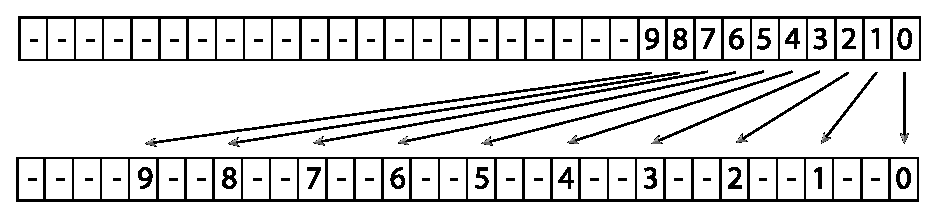
\includegraphics[width=0.75\linewidth]{chap04/LeftShift3.eps}
    \caption{移位以计算3D莫顿码。函数\refvar{LeftShift3}{()}接收32位整数值,
        且对于低10位,把第$i$位移到第$3i$位的位置——换句话说,向左移$2i$位。剩下全部位设为零。}
    \label{fig:4.9}
\end{figure}

实现该操作最明显的方法,即单独移动每一位,并不是最高效的
(它需要总共9次位移以及逻辑或来计算最终值)。
取而代之的是,我们可以把每位的移动分解为多个幂2尺寸的移位且一并把数位值移到其最终位置。
然后,所有需要移动给定幂2数位的位可以一并移动。
函数\refvar{LeftShift3}{()}实现了该计算,\reffig{4.10}展示了它如何工作的。
\begin{figure}[htbp]
    \centering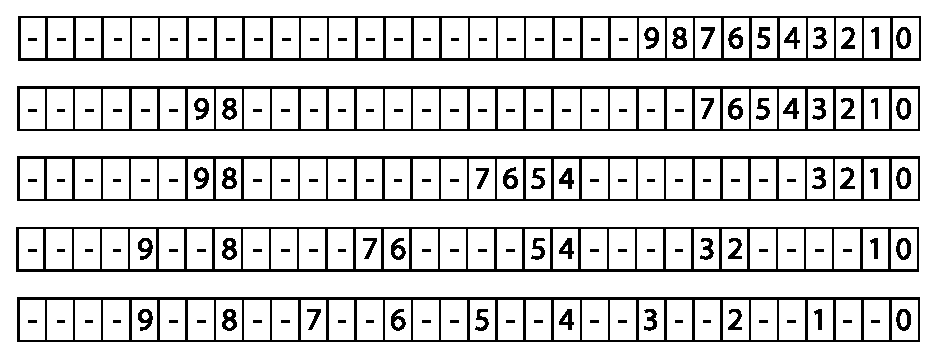
\includegraphics[width=0.75\linewidth]{Pictures/chap04/Mortonpow2decomposition.eps}
    \caption{莫顿移位的幂2分解。通过一系列幂2尺寸的移动来为每个3D坐标计算莫顿码执行移位。
        首先,位8和9向左移16位,这把位8放在了其最终位置。接着位4到7移动8位。
        移动4和2位后(适当掩模使每位最终都移动适当数位),所有数位都在正确的位置上。
        该计算由函数\refvar{LeftShift3}{()}实现。}
    \label{fig:4.10}
\end{figure}

\begin{lstlisting}
`\initcode{BVHAccel Utility Functions}{=}\initnext{BVHAccelUtilityFunctions}`
inline uint32_t `\initvar{LeftShift3}{}`(uint32_t x) {
    if (x == (1 << 10)) --x;
    x = (x | (x << 16)) & 0b00000011000000000000000011111111;
    x = (x | (x <<  8)) & 0b00000011000000001111000000001111;
    x = (x | (x <<  4)) & 0b00000011000011000011000011000011;
    x = (x | (x <<  2)) & 0b00001001001001001001001001001001;
    return x;
}
\end{lstlisting}

\refvar{EncodeMorton3}{()}接收每个分量都是$0$到$2^{10}$之间浮点值的3D坐标值。
它把这些值转换为整数然后通过展开三个10位量化值使第$i$位在位置$3i$上来计算莫顿码,
然后$y$位再移一位,$z$位再移两位,全部结果求或(\reffig{4.11})。
\begin{figure}[htbp]
    \centering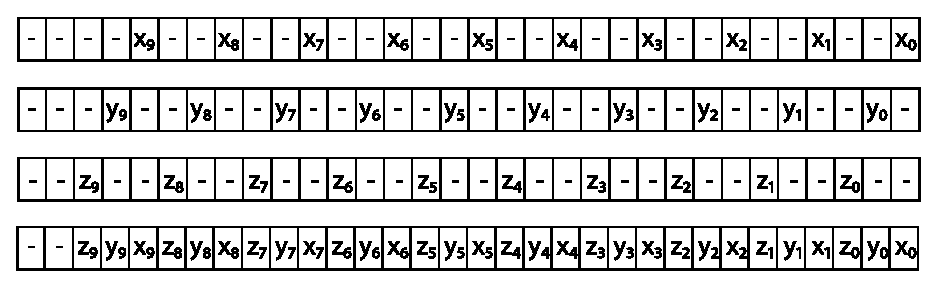
\includegraphics[width=0.75\linewidth]{chap04/Mortonxyzinterleave.eps}
    \caption{最终交错坐标值。有了\refvar{LeftShift3}{()}为$x$、$y$和$z$计算的交错值,
        最终莫顿编码值通过分别移动$y$和$z$一位和两位然后全部结果求或算得。}
    \label{fig:4.11}
\end{figure}

\begin{lstlisting}
`\refcode{BVHAccel Utility Functions}{+=}\lastnext{BVHAccelUtilityFunctions}`
inline uint32_t `\initvar{EncodeMorton3}{}`(const `\refvar{Vector3f}{}` &v) {
    return (`\refvar{LeftShift3}{}`(v.z) << 2) | (`\refvar{LeftShift3}{}`(v.y) << 1) |
            `\refvar{LeftShift3}{}`(v.x);
}
\end{lstlisting}

一旦计算了莫顿索引,我们将用\keyindex{基数排序}{radix sort}{}按莫顿索引值对
\newline{\ttfamily mortonPrims}排序。
我们已经发现对于BVH的构建,我们的基数排序实现明显快于使用我们系统标准库的{\ttfamily std::sort()}
(它是\keyindex{快速排序}{quicksort}{}和\keyindex{插入排序}{insertion sort}{}的混合)。
\begin{lstlisting}
`\initcode{Radix sort primitive Morton indices}{=}`
`\refvar{RadixSort}{}`(&mortonPrims);
\end{lstlisting}

回想基数排序和大多数排序算法的不同在于它不是基于比较一对值
而是基于依赖一些键值的桶子项。基数排序可用于排序整数值,
它从最右边数位到最左边每次排序一个数码。
它尤其值得每次对二进制值排序多个数码;
这样做减少了传递数据的次数。
这里的实现中,{\ttfamily bitsPerPass}设置每次传递处理的位数;
取值6后,我们有5次传递来排序30位。
\begin{lstlisting}
`\refcode{BVHAccel Utility Functions}{+=}\lastcode{BVHAccelUtilityFunctions}`
static void `\initvar{RadixSort}{}`(std::vector<`\refvar{MortonPrimitive}{}`> *v) {
    std::vector<`\refvar{MortonPrimitive}{}`> tempVector(v->size());
    constexpr int bitsPerPass = 6;
    constexpr int nBits = 30;
    constexpr int nPasses = nBits / bitsPerPass;
    for (int pass = 0; pass < nPasses; ++pass) {
        `\refcode{Perform one pass of radix sort, sorting bitsPerPass bits}{}`
    }
    `\refcode{Copy final result from tempVector, if needed}{}`
}
\end{lstlisting}

当前传递会排序{\ttfamily bitsPerPass}位,从{\ttfamily lowBit}开始。
\begin{lstlisting}
`\initcode{Perform one pass of radix sort, sorting bitsPerPass bits}{=}`
int lowBit = pass * bitsPerPass;
`\refcode{Set in and out vector pointers for radix sort pass}{}`
`\refcode{Count number of zero bits in array for current radix sort bit}{}`
`\refcode{Compute starting index in output array for each bucket}{}`
`\refcode{Store sorted values in output array}{}`
\end{lstlisting}

{\ttfamily in}和{\ttfamily out}引用分别对应于要排序的向量以及保存排序值的向量。
每次通过循环的传递都在输入向量{\ttfamily *v}和临时向量之间交替。
\begin{lstlisting}
`\initcode{Set in and out vector pointers for radix sort pass}{=}`
std::vector<`\refvar{MortonPrimitive}{}`> &in  = (pass & 1) ? tempVector : *v;
std::vector<`\refvar{MortonPrimitive}{}`> &out = (pass & 1) ? *v : tempVector;
\end{lstlisting}

如果我们每次传递中排序$n$位,则每个值可能落入的桶有$2^n$个。
我们先计数每个桶中会落入多少个值;这能让我们确定在输出数组中的何处保存排序值。
为了给当前值计算桶索引,该实现对索引移位使得在索引{\ttfamily lowBit}上的位
位于0号位,再掩模低处{\ttfamily bitsPerPass}个位。
\begin{lstlisting}
`\initcode{Count number of zero bits in array for current radix sort bit}{=}`
constexpr int nBuckets = 1 << bitsPerPass;
int bucketCount[nBuckets] = { 0 };
constexpr int bitMask = (1 << bitsPerPass) - 1;
for (const `\refvar{MortonPrimitive}{}` &mp : in) {
    int bucket = (mp.`\refvar{mortonCode}{}` >> lowBit) & bitMask;
    ++bucketCount[bucket];
}
\end{lstlisting}

有了每个桶中落入值的数量,我们就可以计算在输出数组中
每个桶的值开始处的偏移量;这就是之前的桶中落入值数量的和。
\begin{lstlisting}
`\initcode{Compute starting index in output array for each bucket}{=}`
int outIndex[nBuckets];
outIndex[0] = 0;
for (int i = 1; i < nBuckets; ++i)
    outIndex[i] = outIndex[i - 1] + bucketCount[i - 1];
\end{lstlisting}

现在我们知道每个桶在何处开始排序值了,
可以接收另一次图元传递来重算每个图元所在的桶并
将其\refvar{MortonPrimitive}{}保存在输出数组中。
这为当前这组数位完成了排序传递。
\begin{lstlisting}
`\initcode{Store sorted values in output array}{=}`
for (const `\refvar{MortonPrimitive}{}` &mp : in) {
    int bucket = (mp.`\refvar{mortonCode}{}` >> lowBit) & bitMask;
    out[outIndex[bucket]++] = mp;
}
\end{lstlisting}

当完成排序时,如果执行了奇数次基数排序传递,则最终排序值需要
从临时向量复制到原来传入\refvar{RadixSort}{()}的输出向量。
\begin{lstlisting}
`\initcode{Copy final result from tempVector, if needed}{}`
if (nPasses & 1)
    std::swap(*v, tempVector);
\end{lstlisting}

有了图元排序数组,我们将用附近的形心求得图元群集,
再在每个群集内创建图元上的LBVH。
这一步很适合并行化,因为通常有很多群集且每个群集都可以独立处理。
\begin{lstlisting}
`\initcode{Create LBVH treelets at bottom of BVH}{=}`
`\refcode{Find intervals of primitives for each treelet}{}`
`\refcode{Create LBVHs for treelets in parallel}{}`
\end{lstlisting}

每个图元群集都表示为一个\refvar{LBVHTreelet}{}。
它对群集中第一个图元在{\ttfamily mortonPrims}数组中的索引
以及后续图元的数量进行编码(见\reffig{4.12})。
\begin{lstlisting}
`\refcode{BVHAccel Local Declarations}{+=}\lastnext{BVHAccelLocalDeclarations}`
struct `\initvar{LBVHTreelet}{}` {
   int `\initvar{startIndex}{}`, `\initvar[LBVHTreelet:nPrimitives]{nPrimitives}{}`;
   `\refvar{BVHBuildNode}{}` *`\initvar{buildNodes}{}`;
};
\end{lstlisting}

\begin{figure}[htbp]
    \centering%LaTeX with PSTricks extensions
%%Creator: Inkscape 1.0.1 (3bc2e813f5, 2020-09-07)
%%Please note this file requires PSTricks extensions
\psset{xunit=.5pt,yunit=.5pt,runit=.5pt}
\begin{pspicture}(218.83000183,217.97000122)
{
\newrgbcolor{curcolor}{0 0 0}
\pscustom[linewidth=1,linecolor=curcolor]
{
\newpath
\moveto(0.5,217.47000122)
\lineto(217.47000122,217.47000122)
\lineto(217.47000122,0.5)
\lineto(0.5,0.5)
\closepath
}
}
{
\newrgbcolor{curcolor}{0 0 0}
\pscustom[linewidth=1,linecolor=curcolor]
{
\newpath
\moveto(54.66999817,217.83000122)
\lineto(54.66999817,0.74000549)
}
}
{
\newrgbcolor{curcolor}{0 0 0}
\pscustom[linewidth=1,linecolor=curcolor]
{
\newpath
\moveto(108.94000244,217.83000122)
\lineto(108.94000244,0.91000366)
}
}
{
\newrgbcolor{curcolor}{0 0 0}
\pscustom[linewidth=1,linecolor=curcolor]
{
\newpath
\moveto(163.19999695,217.83000122)
\lineto(163.19999695,0.30999756)
}
}
{
\newrgbcolor{curcolor}{0 0 0}
\pscustom[linewidth=1,linecolor=curcolor]
{
\newpath
\moveto(0.80000001,55.41000366)
\lineto(217.47999573,55.41000366)
}
}
{
\newrgbcolor{curcolor}{0 0 0}
\pscustom[linewidth=1,linecolor=curcolor]
{
\newpath
\moveto(0.68000001,109.66999817)
\lineto(217.25999451,109.66999817)
}
}
{
\newrgbcolor{curcolor}{0 0 0}
\pscustom[linewidth=1,linecolor=curcolor]
{
\newpath
\moveto(0.68000001,163.94000244)
\lineto(217.36999512,163.94000244)
}
}
{
\newrgbcolor{curcolor}{0 0 0}
\pscustom[linestyle=none,fillstyle=solid,fillcolor=curcolor]
{
\newpath
\moveto(128.87000036,82.82000732)
\curveto(128.87000036,86.10767491)(124.89535904,87.75354909)(122.57090879,85.42909884)
\curveto(120.24645854,83.10464859)(121.89233272,79.13000727)(125.18000031,79.13000727)
\curveto(128.46766789,79.13000727)(130.11354207,83.10464859)(127.78909182,85.42909884)
\curveto(125.46464157,87.75354909)(121.49000025,86.10767491)(121.49000025,82.82000732)
\curveto(121.49000025,79.53233974)(125.46464157,77.88646556)(127.78909182,80.21091581)
\curveto(130.11354207,82.53536606)(128.46766789,86.51000738)(125.18000031,86.51000738)
\curveto(121.89233272,86.51000738)(120.24645854,82.53536606)(122.57090879,80.21091581)
\curveto(124.89535904,77.88646556)(128.87000036,79.53233974)(128.87000036,82.82000732)
\closepath
}
}
{
\newrgbcolor{curcolor}{0 0 0}
\pscustom[linewidth=1,linecolor=curcolor,linestyle=dashed,dash=2]
{
\newpath
\moveto(106.09999847,96.31999969)
\lineto(143.87999725,96.31999969)
\lineto(143.87999725,69.21999931)
\lineto(106.09999847,69.21999931)
\closepath
}
}
{
\newrgbcolor{curcolor}{0 0 0}
\pscustom[linestyle=none,fillstyle=solid,fillcolor=curcolor]
{
\newpath
\moveto(76.74999762,150.77999878)
\curveto(76.74999762,154.06766637)(72.77535629,155.71354055)(70.45090604,153.3890903)
\curveto(68.12645579,151.06464005)(69.77232997,147.08999872)(73.05999756,147.08999872)
\curveto(76.34766514,147.08999872)(77.99353933,151.06464005)(75.66908908,153.3890903)
\curveto(73.34463883,155.71354055)(69.3699975,154.06766637)(69.3699975,150.77999878)
\curveto(69.3699975,147.49233119)(73.34463883,145.84645701)(75.66908908,148.17090726)
\curveto(77.99353933,150.49535751)(76.34766514,154.46999884)(73.05999756,154.46999884)
\curveto(69.77232997,154.46999884)(68.12645579,150.49535751)(70.45090604,148.17090726)
\curveto(72.77535629,145.84645701)(76.74999762,147.49233119)(76.74999762,150.77999878)
\closepath
}
}
{
\newrgbcolor{curcolor}{0 0 0}
\pscustom[linestyle=none,fillstyle=solid,fillcolor=curcolor]
{
\newpath
\moveto(179.88999701,139.84000397)
\curveto(179.88999701,143.12767155)(175.91535568,144.77354574)(173.59090543,142.44909549)
\curveto(171.26645518,140.12464524)(172.91232936,136.15000391)(176.19999695,136.15000391)
\curveto(179.48766453,136.15000391)(181.13353872,140.12464524)(178.80908847,142.44909549)
\curveto(176.48463822,144.77354574)(172.50999689,143.12767155)(172.50999689,139.84000397)
\curveto(172.50999689,136.55233638)(176.48463822,134.9064622)(178.80908847,137.23091245)
\curveto(181.13353872,139.5553627)(179.48766453,143.53000402)(176.19999695,143.53000402)
\curveto(172.91232936,143.53000402)(171.26645518,139.5553627)(173.59090543,137.23091245)
\curveto(175.91535568,134.9064622)(179.88999701,136.55233638)(179.88999701,139.84000397)
\closepath
}
}
{
\newrgbcolor{curcolor}{0 0 0}
\pscustom[linestyle=none,fillstyle=solid,fillcolor=curcolor]
{
\newpath
\moveto(44.64999914,38.22000122)
\curveto(44.64999914,41.50766881)(40.67535782,43.15354299)(38.35090757,40.82909274)
\curveto(36.02645732,38.50464249)(37.6723315,34.53000116)(40.95999908,34.53000116)
\curveto(44.24766667,34.53000116)(45.89354085,38.50464249)(43.5690906,40.82909274)
\curveto(41.24464035,43.15354299)(37.26999903,41.50766881)(37.26999903,38.22000122)
\curveto(37.26999903,34.93233363)(41.24464035,33.28645945)(43.5690906,35.6109097)
\curveto(45.89354085,37.93535995)(44.24766667,41.91000128)(40.95999908,41.91000128)
\curveto(37.6723315,41.91000128)(36.02645732,37.93535995)(38.35090757,35.6109097)
\curveto(40.67535782,33.28645945)(44.64999914,34.93233363)(44.64999914,38.22000122)
\closepath
}
}
{
\newrgbcolor{curcolor}{0 0 0}
\pscustom[linestyle=none,fillstyle=solid,fillcolor=curcolor]
{
\newpath
\moveto(143.66999578,199.77000046)
\curveto(143.66999578,203.05766804)(139.69535446,204.70354223)(137.37090421,202.37909198)
\curveto(135.04645396,200.05464173)(136.69232814,196.0800004)(139.97999573,196.0800004)
\curveto(143.26766331,196.0800004)(144.9135375,200.05464173)(142.58908725,202.37909198)
\curveto(140.264637,204.70354223)(136.28999567,203.05766804)(136.28999567,199.77000046)
\curveto(136.28999567,196.48233287)(140.264637,194.83645869)(142.58908725,197.16090894)
\curveto(144.9135375,199.48535919)(143.26766331,203.46000051)(139.97999573,203.46000051)
\curveto(136.69232814,203.46000051)(135.04645396,199.48535919)(137.37090421,197.16090894)
\curveto(139.69535446,194.83645869)(143.66999578,196.48233287)(143.66999578,199.77000046)
\closepath
}
}
{
\newrgbcolor{curcolor}{0 0 0}
\pscustom[linewidth=1,linecolor=curcolor]
{
\newpath
\moveto(143.66999578,199.77000046)
\curveto(143.66999578,203.05766804)(139.69535446,204.70354223)(137.37090421,202.37909198)
\curveto(135.04645396,200.05464173)(136.69232814,196.0800004)(139.97999573,196.0800004)
\curveto(143.26766331,196.0800004)(144.9135375,200.05464173)(142.58908725,202.37909198)
\curveto(140.264637,204.70354223)(136.28999567,203.05766804)(136.28999567,199.77000046)
\curveto(136.28999567,196.48233287)(140.264637,194.83645869)(142.58908725,197.16090894)
\curveto(144.9135375,199.48535919)(143.26766331,203.46000051)(139.97999573,203.46000051)
\curveto(136.69232814,203.46000051)(135.04645396,199.48535919)(137.37090421,197.16090894)
\curveto(139.69535446,194.83645869)(143.66999578,196.48233287)(143.66999578,199.77000046)
\closepath
}
}
{
\newrgbcolor{curcolor}{0 0 0}
\pscustom[linewidth=1,linecolor=curcolor,linestyle=dashed,dash=2]
{
\newpath
\moveto(123.81999969,214.10000134)
\lineto(155.86999893,214.10000134)
\lineto(155.86999893,185.96000195)
\lineto(123.81999969,185.96000195)
\closepath
}
}
{
\newrgbcolor{curcolor}{0 0 0}
\pscustom[linewidth=1,linecolor=curcolor,linestyle=dashed,dash=2]
{
\newpath
\moveto(33.40000153,171.63000107)
\lineto(113.13999939,171.63000107)
\lineto(113.13999939,130.4600029)
\lineto(33.40000153,130.4600029)
\closepath
}
}
{
\newrgbcolor{curcolor}{0 0 0}
\pscustom[linewidth=1,linecolor=curcolor,linestyle=dashed,dash=2]
{
\newpath
\moveto(167.86000061,162.25)
\lineto(184.28000069,162.25)
\lineto(184.28000069,117.95000076)
\lineto(167.86000061,117.95000076)
\closepath
}
}
{
\newrgbcolor{curcolor}{0 0 0}
\pscustom[linewidth=1,linecolor=curcolor,linestyle=dashed,dash=2]
{
\newpath
\moveto(18.29000092,64.80000305)
\lineto(63.37000275,64.80000305)
\lineto(63.37000275,11.6400032)
\lineto(18.29000092,11.6400032)
\closepath
}
}
\end{pspicture}

    \caption{LBVH小树的图元群集。图元形心聚类到覆盖其边界的均匀网格内。
        为每个格子中位于排序后的莫顿索引值连续段内的图元群集创建LBVH。}
    \label{fig:4.12}
\end{figure}

回想\reffig{4.8}中,莫顿码高位值匹配的点集位于原始盒中一个幂2对齐和幂2边长的子集内。
因为我们已经用莫顿编码值对数组{\ttfamily mortonPrims}排过序了,
所以高位值匹配的图元已经位于一段连续数组中。

这里我们将求30位莫顿码中有相同的高12位对应的图元集。
通过线性浏览数组{\ttfamily mortonPrims}来求得群集并
找到这12位中有任何一位发生变化的地方。
这对应了在$2^{12}=4096$个规范网格中对图元聚类,
每维有$2^4=16$个格子。
实践中,许多网格是空的,
尽管这里我们仍然希望求得许多独立的群集。
\begin{lstlisting}
`\initcode{Find intervals of primitives for each treelet}{=}`
std::vector<`\refvar{LBVHTreelet}{}`> treeletsToBuild;
for (int start = 0, end = 1; end <= (int)mortonPrims.size(); ++end) {
    uint32_t mask = 0b00111111111111000000000000000000;
    if (end == (int)mortonPrims.size() ||
        ((mortonPrims[start].`\refvar{mortonCode}{}` & mask) !=
         (mortonPrims[end].`\refvar{mortonCode}{}` & mask))) {
        `\refcode{Add entry to treeletsToBuild for this treelet}{}`
        start = end;
    }
}
\end{lstlisting}

当为一个小树求得一个图元群集后,就立即为它分配\refvar{BVHBuildNode}{}
(回想一个BVH中的节点数量不超过叶子节点数量的两倍,而后者又不超过图元数量)。
在现在的串行执行阶段中预分配这些内存比在LBVH的并行构建中分配更简单。

这里的一个重要细节是传入\refvar[MemoryArena:Alloc2]{MemoryArena::Alloc}{()}的{\ttfamily false}值;
它表示不要执行正在分配的底层对象的构造函数。
令人惊讶的是,运行\refvar{BVHBuildNode}{}构造函数会引入很大开销
并明显降低构建HLBVH时的整体性能。
因为在后面的代码中\refvar{BVHBuildNode}{}的所有成员都会初始化,
所以无论如何这里都没必要用构造函数执行初始化。

\begin{lstlisting}
`\initcode{Add entry to treeletsToBuild for this treelet}{=}`
int nPrimitives = end - start;
int maxBVHNodes = 2 * nPrimitives - 1;
`\refvar{BVHBuildNode}{}` *nodes = arena.`\refvar[MemoryArena:Alloc2]{Alloc}{}`<`\refvar{BVHBuildNode}{}`>(maxBVHNodes, false);
treeletsToBuild.push_back({start, nPrimitives, nodes});
\end{lstlisting}

一旦每个小树的图元都定好了,我们就可以并行地为它们创建LBVH了。
当构建完成后,每个\refvar{LBVHTreelet}{}的指针\refvar{buildNodes}{}会指向相应LBVH的根。

工作线程在构建LBVH时有两个地方必须相互配合。
第一,需要计算所有LBVH中的节点总数并通过传入\refvar{HLBVHBuild}{()}的
指针{\ttfamily totalNode}返回。
第二,当为LBVH创建叶子节点时,
需要数组{\ttfamily orderedPrims}的连续一段来
记录叶子节点中图元的索引。
我们的实现为两者都使用了原子变量——
{\ttfamily atomicTotal}跟踪节点的数目,
{\ttfamily orderedPrimsOffset}跟踪{\ttfamily orderedPrims}下一有效项的索引。
\begin{lstlisting}
`\initcode{Create LBVHs for treelets in parallel}{=}`
std::atomic<int> atomicTotal(0), orderedPrimsOffset(0);
orderedPrims.resize(primitives.size());
`\refvar{ParallelFor}{}`(
    [&](int i) {
        `\refcode{Generate ith LBVH treelet}{}`
    }, treeletsToBuild.size());
*totalNodes = atomicTotal;
\end{lstlisting}

构建小树的工作由\refvar{emitLBVH}{()}执行,
它取用形心位于某空间区域内的图元并不断用划分平面
沿着三轴之一上的区域中心将当前空间区域划分为两半。

注意到\refvar{emitLBVH}{()}没有用
指向原子变量{\ttfamily atomicTotal}的指针来计数创建的节点,
而是更新一个非原子局部变量。
然后当每棵小树建成时这里的代码片只对每棵小树更新一次{\ttfamily atomicTotal}。
该方法比让工作线程在其执行过程中频繁修改{\ttfamily atomicTotal}具有明显更好的性能
(见附录\refsub{内存连续模型与性能}关于多核内存连续模型开销的讨论)。
\begin{lstlisting}
`\initcode{Generate ith LBVH treelet}{=}`
int nodesCreated = 0;
const int firstBitIndex = 29 - 12;
`\refvar{LBVHTreelet}{}` &tr = treeletsToBuild[i];
tr.`\refvar{buildNodes}{}` = 
    `\refvar{emitLBVH}{}`(tr.`\refvar{buildNodes}{}`, primitiveInfo, &mortonPrims[tr.`\refvar{startIndex}{}`],
             tr.`\refvar[LBVHTreelet:nPrimitives]{nPrimitives}{}`, &nodesCreated, orderedPrims,
             &orderedPrimsOffset, firstBitIndex);
atomicTotal += nodesCreated;
\end{lstlisting}

幸好有莫顿编码,当前空间区域不需要在\refvar{emitLBVH}{()}中显式表示:
传入的有序{\ttfamily mortonPrims}有一些匹配的高位,反过来对应了一个空间框。
对于莫顿码中剩下的每一位,该函数尝试沿着对应于数位{\ttfamily bitIndex}的平面来划分图元
(回想\reffig{4.8}(d)),然后再递归地调用自己。
尝试用来划分的下一位索引被作为该函数的最后一个参数传入:它最初为$29-12$,
因为29是从零计起的第30位索引,而我们之前用了高12位莫顿码值来聚类图元;
所以,我们知道那些数位都一定匹配该群集。
\begin{lstlisting}
`\refcode{BVHAccel Method Definitions}{+=}\lastnext{BVHAccelMethodDefinitions}`
`\refvar{BVHBuildNode}{}` *`\refvar{BVHAccel}{}`::`\initvar{emitLBVH}{}`(`\refvar{BVHBuildNode}{}` *&buildNodes,
        const std::vector<`\refvar{BVHPrimitiveInfo}{}`> &primitiveInfo,
        `\refvar{MortonPrimitive}{}` *mortonPrims, int nPrimitives, int *totalNodes,
        std::vector<std::shared_ptr<`\refvar{Primitive}{}`>> &orderedPrims,
        std::atomic<int> *orderedPrimsOffset, int bitIndex) const {
    if (bitIndex == -1 || nPrimitives < maxPrimsInNode) {
        `\refcode{Create and return leaf node of LBVH treelet}{}`
    } else {
        int mask = 1 << bitIndex;
        `\refcode{Advance to next subtree level if there's no LBVH split for this bit}{}`
        `\refcode{Find LBVH split point for this dimension}{}`
        `\refcode{Create and return interior LBVH node}{}`
    }
}
\end{lstlisting}

在\refvar{emitLBVH}{()}用最后低位划分完图元后,
不可能再有更多划分了,就创建一个叶子节点。
或者它也可以在只有很少的图元时就停止并创建叶子节点。

回想{\ttfamily orderedPrimsOffset}是数组{\ttfamily orderedPrims}中
下一有效元素的偏置量。
这里,对{\ttfamily fetch\_add()}的调用原子地将{\ttfamily nPrimitives}的值加到\newline
{\ttfamily orderedPrimsOffset}上并返回相加前它的旧值。
因为这些计算是原子的,多个LBVH构建线程可以
同时分割数组{\ttfamily orderedPrims}中的空间且没有数据竞争。
有了数组中的空间,叶子的构建和之前\refcode{Create leaf BVHBuildNode}{}中实现的方法一样。
\begin{lstlisting}
`\initcode{Create and return leaf node of LBVH treelet}{=}`
(*totalNodes)++;
`\refvar{BVHBuildNode}{}` *node = buildNodes++;
`\refvar{Bounds3f}{}` bounds;
int firstPrimOffset = orderedPrimsOffset->fetch_add(nPrimitives);
for (int i = 0; i < nPrimitives; ++i) {
    int primitiveIndex = mortonPrims[i].`\refvar{primitiveIndex}{}`;
    orderedPrims[firstPrimOffset + i] = primitives[primitiveIndex];
    bounds = `\refvar[Union2]{Union}{}`(bounds, primitiveInfo[primitiveIndex].`\refvar[BVHPrimitiveInfo::bounds]{bounds}{}`);
}
node->`\refvar{InitLeaf}{}`(firstPrimOffset, nPrimitives, bounds);
return node;
\end{lstlisting}

可能有所有图元都位于划分平面同一侧的情况;因为图元按其莫顿索引排序,
可以通过看该范围内第一个和最后一个图元对于该平面是否有相同的数位来高效检测该情况。
这种情况下,\refvar{emitLBVH}{()}行进到下一位而不会无用地创建一个节点。
\begin{lstlisting}
`\initcode{Advance to next subtree level if there's no LBVH split for this bit}{=}`
if ((mortonPrims[0].`\refvar{mortonCode}{}` & mask) ==
    (mortonPrims[nPrimitives - 1].`\refvar{mortonCode}{}` & mask))
    return `\refvar{emitLBVH}{}`(buildNodes, primitiveInfo, mortonPrims, nPrimitives,
                    totalNodes, orderedPrims, orderedPrimsOffset,
                    bitIndex - 1);
\end{lstlisting}

如果划分平面两侧都有图元,则二分搜索会高效地找到
当前图元集中第{\ttfamily bitIndex}位从0变为1的划分点。
\begin{lstlisting}
`\initcode{Find LBVH split point for this dimension}{=}`
int searchStart = 0, searchEnd = nPrimitives - 1;
while (searchStart + 1 != searchEnd) {
    int mid = (searchStart + searchEnd) / 2;
    if ((mortonPrims[searchStart].`\refvar{mortonCode}{}` & mask) ==
        (mortonPrims[mid].`\refvar{mortonCode}{}` & mask))
        searchStart = mid;
    else
        searchEnd = mid;
}
int splitOffset = searchEnd;
\end{lstlisting}

有了划分偏置量,该方法现在可以声明一个节点用作中间节点
并为划出的两个图元集递归地构建LBVH了。
注意到莫顿编码还带来了一个方便:
不需要为了划分而复制或记录数组{\ttfamily mortonPrims}中的项:
因为它们都按莫顿码值排序了且从高到低处理数位,
两部分图元已经在划分平面的正确一侧。
\begin{lstlisting}
`\initcode{Create and return interior LBVH node}{=}`
(*totalNodes)++;
`\refvar{BVHBuildNode}{}` *node = buildNodes++;
`\refvar{BVHBuildNode}{}` *lbvh[2] = {
    `\refvar{emitLBVH}{}`(buildNodes, primitiveInfo, mortonPrims, splitOffset,
             totalNodes, orderedPrims, orderedPrimsOffset, bitIndex - 1),
    `\refvar{emitLBVH}{}`(buildNodes, primitiveInfo, &mortonPrims[splitOffset],
             nPrimitives - splitOffset, totalNodes, orderedPrims,
             orderedPrimsOffset, bitIndex - 1)
};
int axis = bitIndex % 3;
node->`\refvar{InitInterior}{}`(axis, lbvh[0], lbvh[1]);
return node;
\end{lstlisting}

一旦创建好所有LBVH小树,
\refvar{buildUpperSAH}{()}就为所有小树创建一个BVH。
因为它们通常只有几十个或几百个(无论如何不超过4096),
该步骤花的时间很少。
\begin{lstlisting}
`\initcode{Create and return SAH BVH from LBVH treelets}{=}`
std::vector<`\refvar{BVHBuildNode}{}` *> finishedTreelets;
for (`\refvar{LBVHTreelet}{}` &treelet : treeletsToBuild)
    finishedTreelets.push_back(treelet.`\refvar{buildNodes}{}`);
return `\refvar{buildUpperSAH}{}`(arena, finishedTreelets, 0,
                     finishedTreelets.size(), totalNodes);
\end{lstlisting}

这里不介绍该方法的实现,
因为它和完全基于SAH的BVH构建遵循相同的方法,
只不过是在小树根节点上而不是在场景图元上进行。
\begin{lstlisting}
`\initcode{BVHAccel Private Methods}{=}`
`\refvar{BVHBuildNode}{}` *`\initvar{buildUpperSAH}{}`(`\refvar{MemoryArena}{}` &arena,
    std::vector<`\refvar{BVHBuildNode}{}` *> &treeletRoots, int start, int end,
    int *totalNodes) const;
\end{lstlisting}